\documentclass[a5paper,12pt,twoside,openany]{book}
\usepackage[top=2cm, bottom=1.25cm, left=1.5cm, right=1.5cm, bindingoffset=8mm,headsep=5mm]{geometry}
\usepackage{amsmath}
\usepackage{amsthm}
\usepackage{acronym}
\usepackage{grffile}
\usepackage{hyperref}
\usepackage{graphicx}
\usepackage[frenchb]{babel}
\usepackage[utf8]{inputenc}
\usepackage{suffix}
\usepackage{xstring}
\usepackage{url}
\usepackage[T1]{fontenc}
\usepackage{array}
\usepackage{sectsty}
\usepackage[usenames, dvipsnames]{color}
\usepackage[official]{eurosym}



\DeclareUnicodeCharacter{20AC}{\euro}
\DeclareUnicodeCharacter{B4}{'}
\DeclareUnicodeCharacter{14D}{\={o}}
\DeclareUnicodeCharacter{FF1A}{:}
\DeclareUnicodeCharacter{FF01}{!}
\DeclareUnicodeCharacter{16B}{\={u}}
\DeclareUnicodeCharacter{B0}{$^\circ$}
\DeclareUnicodeCharacter{2033}{''}
\DeclareUnicodeCharacter{B5}{$\mu$}

% Font
\renewcommand*\rmdefault{iwona}


% Headers and footers
\usepackage{fancyhdr}
\pagestyle{fancy}
\renewcommand{\headrulewidth}{0pt}
\fancyhf{}
\fancyhead[RO]{\color{RoyalBlue} \it \leftmark}

% Chapter pages style
\fancypagestyle{plain}{\fancyhf{}}
\chapterfont{\color{RoyalBlue}}
\sectionfont{\color{Gray} \large}

% Images width
\def\mywidth{0.9\textwidth}

%%%  CHANGE IMAGE PATH HERE %%%
%\graphicspath{{C:/MyWebSites/Backup/souivezlevelo/images_high/wp-content/}}
\graphicspath{{C:/MyWebSites/Backup/souivezlevelo/images_low/wp-content/}}


\begin{document}
\chapter*{Itinéraire\markboth{Itinéraire}{}}
\section*{26 octobre 2014}

\begin{center}

\includegraphics[width=\mywidth]{../wp-content/uploads/2014/10/7-drapeaux-1024x95.jpg}
\end{center}

Le billet d'avion \og Tour du monde\fg\ est réservé, avec un départ le 8~février~2015 pour un retour le 20~décembre~2015.

 Et voici les dates prévues dans chaque pays. Les billets d'avion étant flexibles, je peux changer les dates des vols à tout moment. 
\begin{itemize}
\item Chili : du 8 février au 1er avril 
\item Bolivie : du 2 avril au 29 avril 
\item Pérou : du 30 avril au 24 juin 
\item Équateur : du 25 juin au 12 juillet 
\item Japon : du 15 juillet au 30 août 
\item Chine : du 31 août au 25 octobre 
\item Inde : du 26 octobre au 20 décembre 
\end{itemize}

\vspace{2mm}

\begin{center}
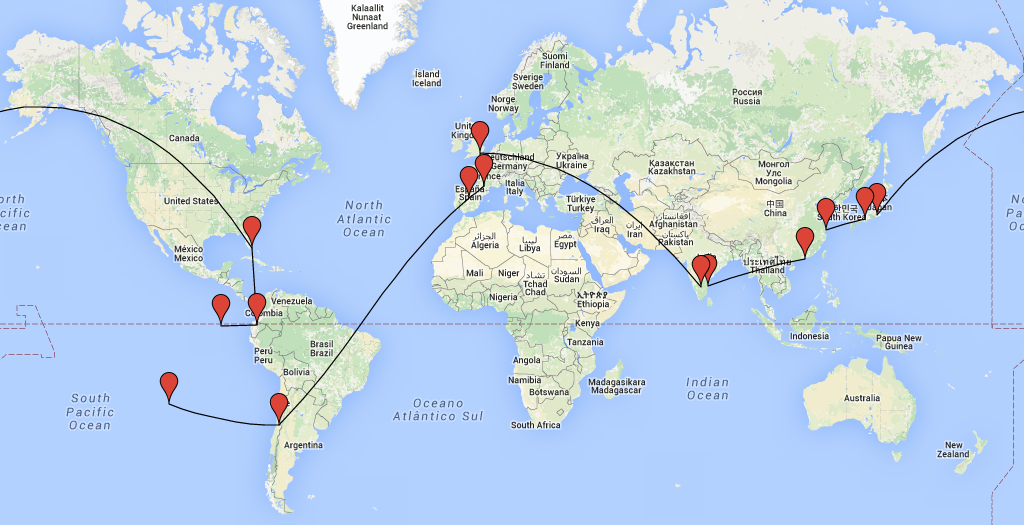
\includegraphics[width=\textwidth]{../wp-content/uploads/2016/01/carte_remi.png}
\end{center}
\chapter*{Le vélo\markboth{Le vélo}{}}
\section*{29 octobre 2014}
Mon objectif est de faire une bonne partie des déplacements en vélo, il me faut donc un vélo adapté au voyage :
\begin{itemize}
\item solide et fiable,
 \item réparable, donc avec des pièces standards,
 \item adapté à la route et aux chemins,
\item à un prix raisonnable.
\end{itemize}

 Les contacts que j'ai eus avec les vendeurs de vélos ne m'ont pas convaincu d'acheter un vélo tout prêt, ni d'en faire monter un sur mesure : prix élevés, configuration du vélo trop haut de gamme ou peu adapté. 
 
 J'ai choisi de monter le vélo en achetant toutes les pièces séparément, ce qui a l'avantage de me donner une bonne connaissance du vélo et du montage. Cela sera sans doute utile à un moment ou à un autre. 
 
 \pagebreak
 J'ai d'abord acheté un VTT d'occasion datant de 1992, principalement à cause du cadre en acier Tange, solide et réparable. En plus, j'ai gardé certaines autres pièces.

\begin{center}
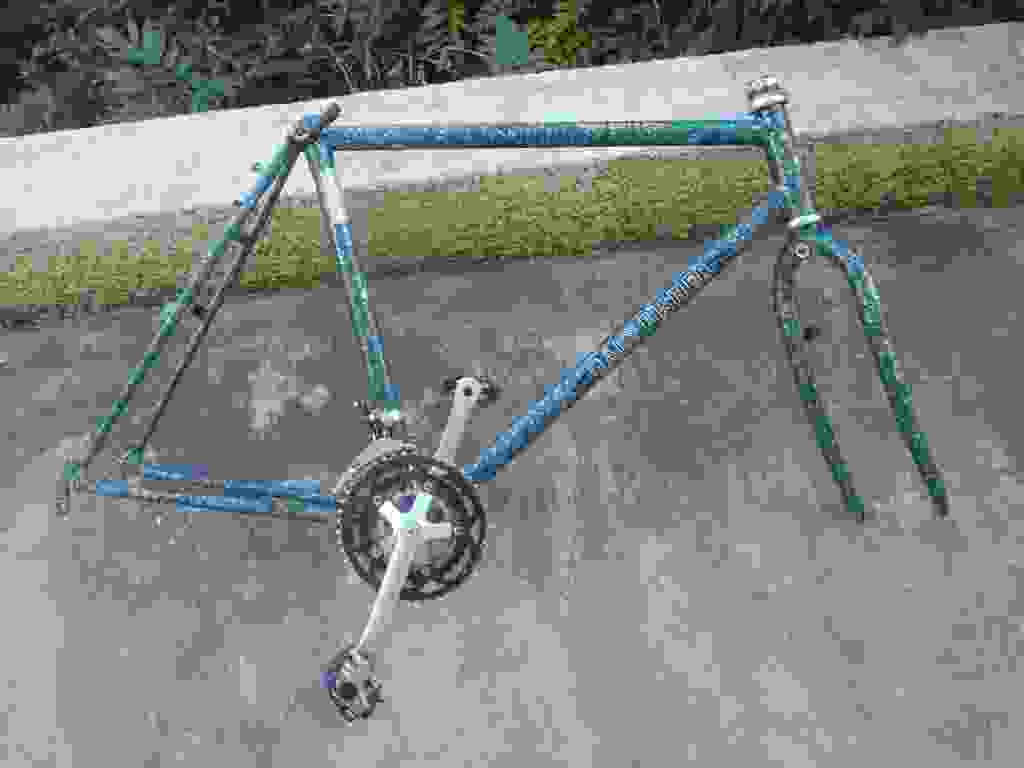
\includegraphics[width=\mywidth]{../wp-content/uploads/2014/10/Cadre.jpg} 
 \end{center}

 J'ai ensuite monté des pièces neuves, que j'ai choisies en m'appuyant sur les conseils que j'ai trouvés sur les blogs ou les forums. 
 
 Et le résultat : 
 
\begin{center}
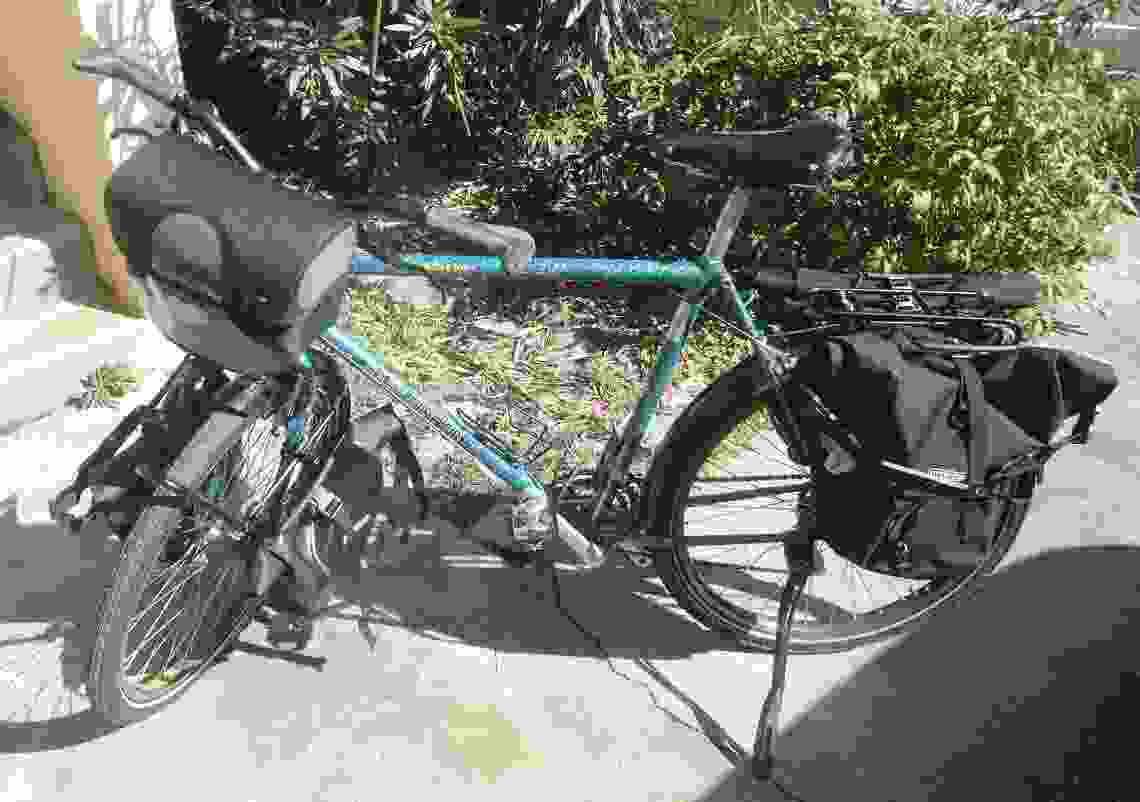
\includegraphics[width=\mywidth]{../wp-content/uploads/2014/10/Velo.jpg} 
\end{center}

 Ça donne un vélo complet pour environ 1000€, sacoches comprises. Voici le détail de la composition du vélo :
 \begin{center}
% \rowcolors{2}{white}{blue}
  \begin{tabular}{ll}
   \bf  Elément & \bf Modèle    \\ 
   \hline
  Cadre + fourche &  Gary Fisher (acier tange)    \\ 
  Jeu de direction &  D'origine du VTT    \\ 
  Potence + plongeur &  BBB Highrise 110mm    \\ 
  Cintre &  Relevé XLC 63cm    \\  
  Poignées &  Ergonomiques avec Bar End intégrés    \\   
  Transmission AV &  Shimano Deore LX d'origine du VTT    \\   
  Plateaux &  D'origine du VTT (petit plateau 24 dents)    \\   
  Transmission AR &  Shimano Acera 7 vitesses    \\   
  Roue libre AR &  7 vitesses 14-34 Megarange    \\   
  Chaîne &  Shimano 6-8 vitesses    \\   
  Freins &  Shimano Acera V-Brake    \\   
  Pédalier &  D'origine du VTT    \\   
  Tige de selle &  D'origine du VTT    \\   
  Selle &  Brook B17 Imperial    \\   
  Roues &  Mavic d'origine du VTT (36 trous, montées main)    \\   
  Pneus &  Schwalbe Marathon Dureme  Mondial    \\   
  Béquille &  Pletscher ESGE    \\   
  Garde-boue &  SKS Chromoplastics    \\   
  Porte-bagages &  Tubus Tara  Logo    \\   
  Sacoches &  Ortlieb Back Roller, Front Roller, Ultimate 6 \\
  \hline
   \end{tabular}
   \end{center}

\chapter*{Sortie de préparation Toulouse – Figeac\markboth{Sortie de préparation Toulouse – Figeac}{}}
\section*{11 novembre 2014}
Première sortie test ce week end. J'ai profité du pont du 11 novembre pour partir avec le vélo, en configuration voyage, direction Figeac.

 L'itinéraire prévu fait environ 200km, faisable sur 2 ou 3 jours, selon le nombre de km que j'arriverai à faire sur une journée.

 Départ dimanche matin à 9h, la pesée de départ vélo chargé avec les affaires, la nourriture pour 3 jours et 3.5L d'eau me donne 41.5kg :
\begin{center} 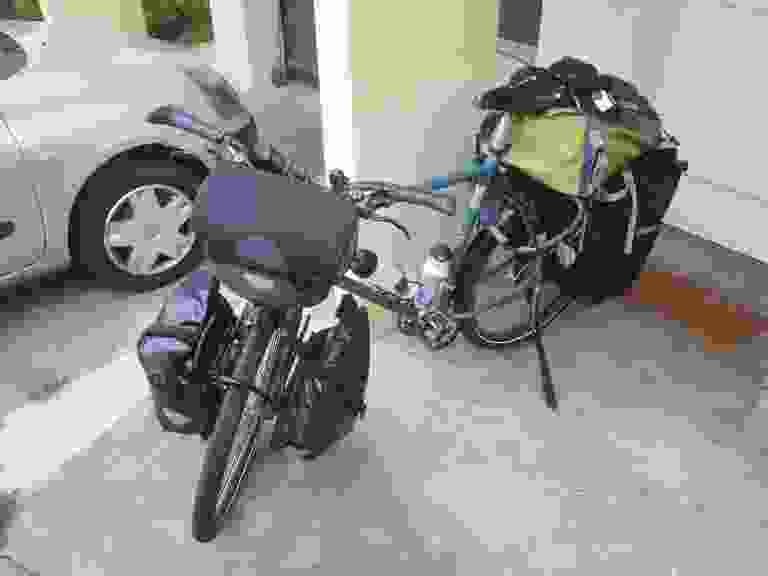
\includegraphics[width=\mywidth]{../wp-content/uploads/2014/11/PB092254.jpg} \end{center}

 Quelques tours de roue dans la rue, et c'est un faux départ car les vitesses que j'avais pourtant bien réglées quelques jours avant ne passent pas bien, ainsi que le frein arrière qui est un peu mou. Retour à la maison pour modifier les réglages. En fait, c'est la sacoche de guidon, en appuyant sur les câbles, qui a déréglée les vitesses.

 Deuxième départ à 10h, cette fois c'est le bon !
Début de l'itinéraire sur le canal latéral direction Bordeaux, 50km de plat pour commencer.
\begin{center} 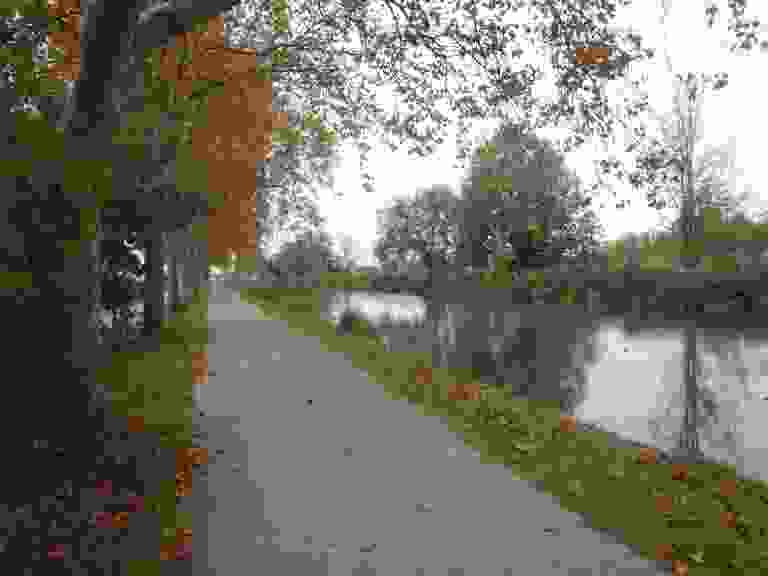
\includegraphics[width=\mywidth]{../wp-content/uploads/2014/11/PB092259.jpg} \end{center}

 Au bout d'une vingtaine de km, la pluie arrive, fine mais régulière.
\begin{center} 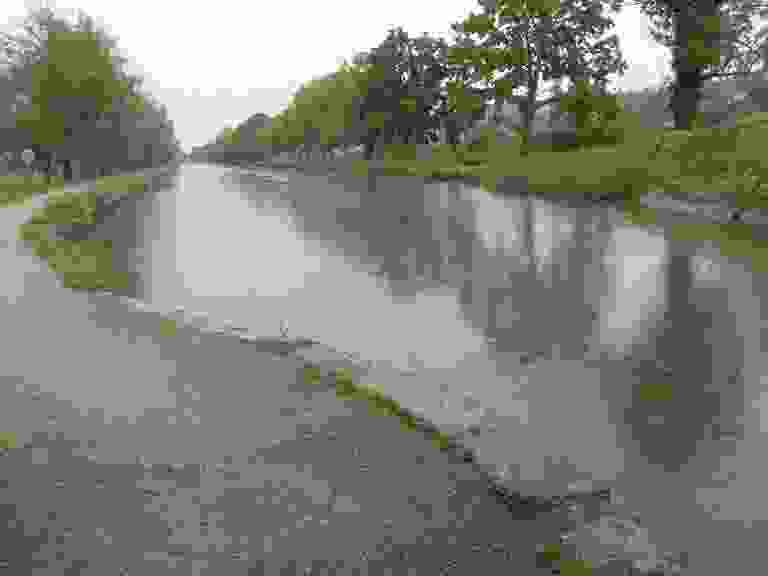
\includegraphics[width=\mywidth]{../wp-content/uploads/2014/11/PB092260.jpg} \end{center}

 J'enfile mes protections de jambes, que je n'ai pas encore testées. Elles sont légères mais plutôt minimalistes, je sais pas ce que ça va donner.
\begin{center} 
\includegraphics[width=\mywidth]{../wp-content/uploads/2014/11/rainlegs02.jpg} \end{center}

Finalement, sous une pluie fine, ininterrompue pendant 3 ou 4h, c'était parfait, la protection jusqu'au genou est suffisante pour avoir les jambes au sec. Il faut juste ne pas oublier d'essuyer la selle quand on remonte sur le vélo après une pause !

 Au bout de 50km, je quitte le canal au niveau de Saint Porquier.
\begin{center} 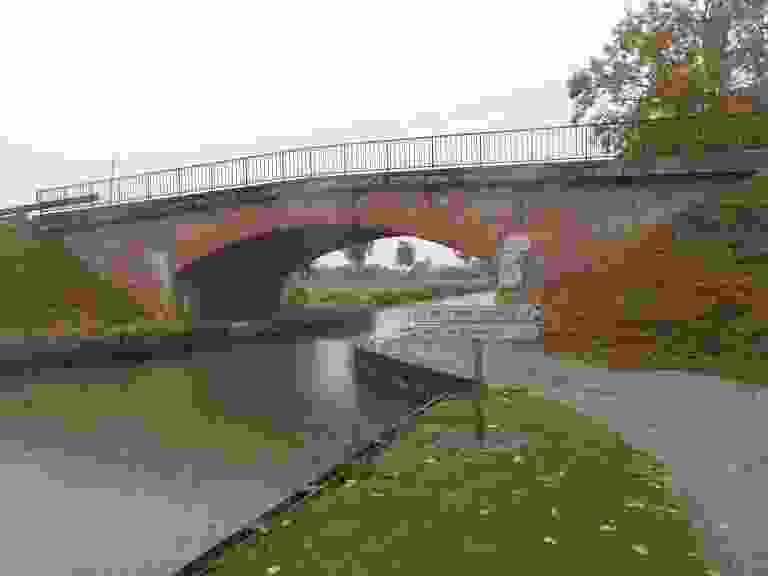
\includegraphics[width=\mywidth]{../wp-content/uploads/2014/11/PB092264.jpg} \end{center}
\begin{center} 
\includegraphics[width=\mywidth]{../wp-content/uploads/2014/11/PB092265.jpg} \end{center}

 Je continue en direction de Ville Dieu du Temple, où je m'arrête pour pique-niquer, à l'abri devant l'entrée de l'école du village.

 Passage par Lafrançaise, après une côte longue et bien raide. J'ai pu tester la petite vitesse du vélo, le 24-34 devrait me permettre de bien passer la plupart des côtes, à 4km/h, ça mouline sans trop d'effort.
 
\begin{center} 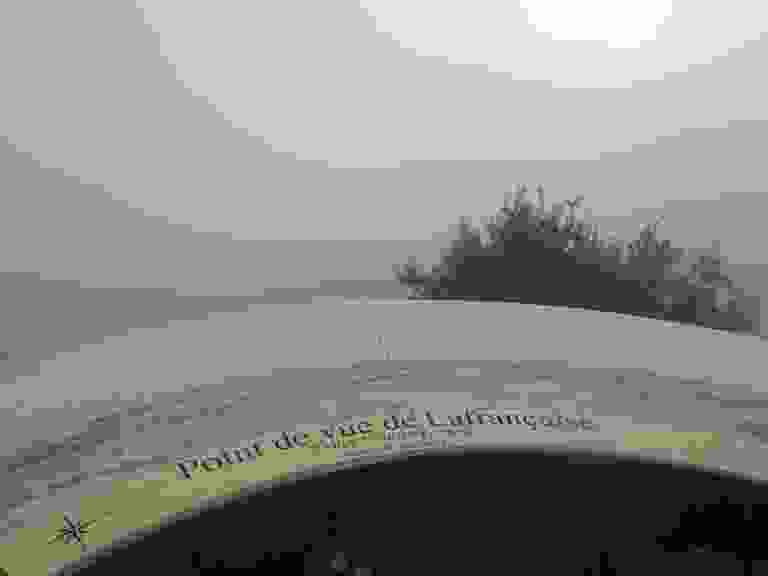
\includegraphics[width=\mywidth]{../wp-content/uploads/2014/11/PB092266.jpg} \end{center}

\pagebreak
 Après presque 90km, j'arrive au niveau de Castelnau Montratier. Il est 17h15, il va être temps de trouver un endroit pour le bivouac.
\begin{center} 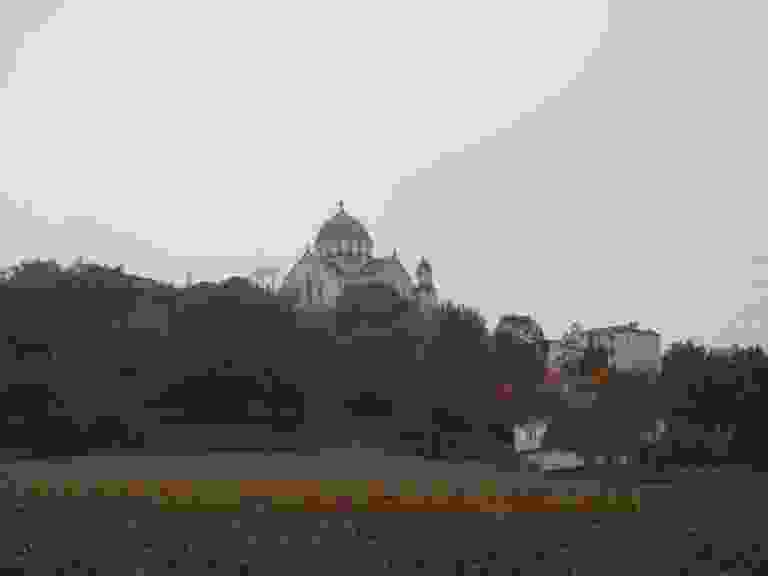
\includegraphics[width=\mywidth]{../wp-content/uploads/2014/11/PB092270.jpg} \end{center}

 Quelques km après la sortie du village, je vois un petit sentier qui monte au bord de la route et je décide d'aller voir ce qu'il y a en haut. Après une centaine de mètres, je tombe sur un emplacement idéal pour passer la nuit.
\begin{center} 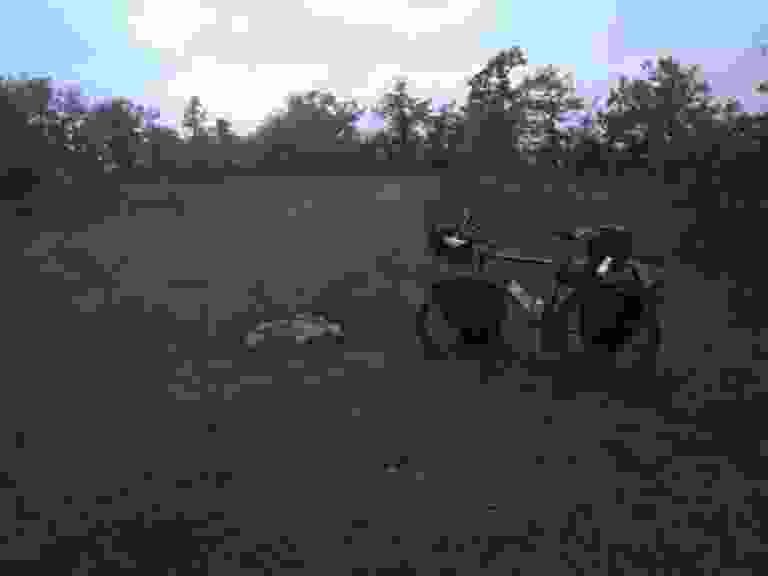
\includegraphics[width=\mywidth]{../wp-content/uploads/2014/11/PB092273.jpg} \end{center}

 J'installe la tente alors que la nuit commence à tomber et heureusement la pluie s'était arrêtée quelques heures avant. 
\begin{center} 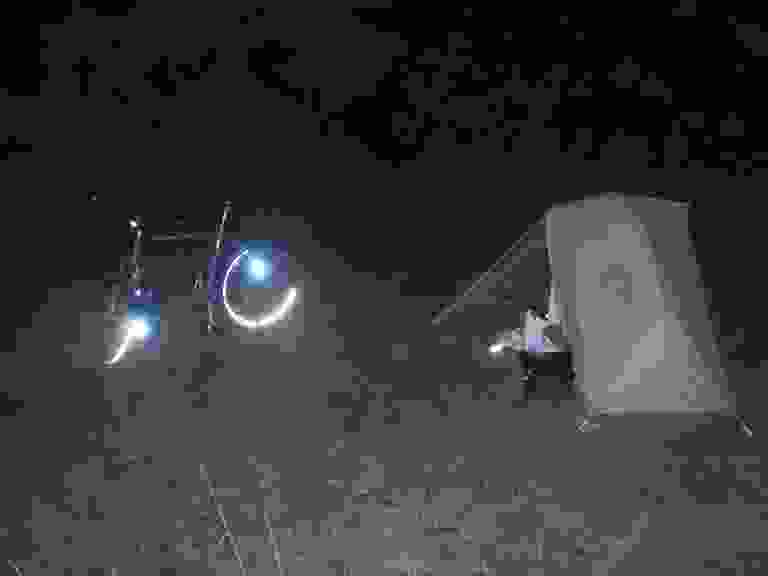
\includegraphics[width=\mywidthreduced]{../wp-content/uploads/2014/11/PB092274.jpg} \end{center}

 Le lendemain matin, départ un peu avant 9h en direction de Cahors. Au bout d'environ 15km, je croise la route nationale et je m'aperçois que je n'ai pas pris la bonne route, j'avais raté une bifurcation la veille juste avant de m'arrêter.
 Du coup, pour éviter de rouler sur la nationale, je décide de changer d'itinéraire et de continuer direction Lalbenque, pour ensuite rejoindre la vallée du Célé au niveau de Saint Cirq Lapopie.
\begin{center} 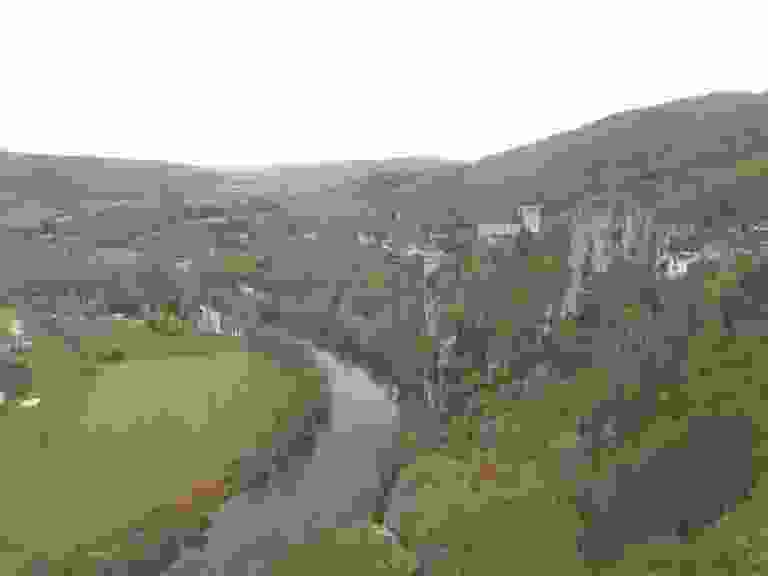
\includegraphics[width=\mywidthreduced]{../wp-content/uploads/2014/11/PB102280.jpg} \end{center}

J'arrive à Saint Cirq Lapopie vers 11h30, par le haut du village.

\begin{center} 
\includegraphics[width=\mywidth]{../wp-content/uploads/2014/11/PB102288.jpg} \end{center}

 J'en profite pour visiter rapidement le plus beau village de France 2012.
 
\begin{center} 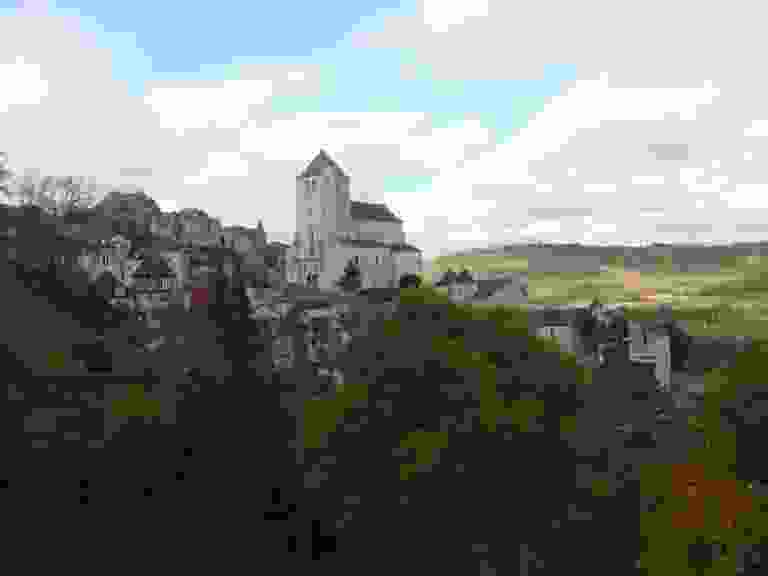
\includegraphics[width=\mywidth]{../wp-content/uploads/2014/11/PB102289.jpg} \end{center}

\pagebreak
 Je descend au bord du Lot en dessous de Saint Cirq Lapopie, afin de rejoindre la vallée du Célé, direction Figeac.
\begin{center} 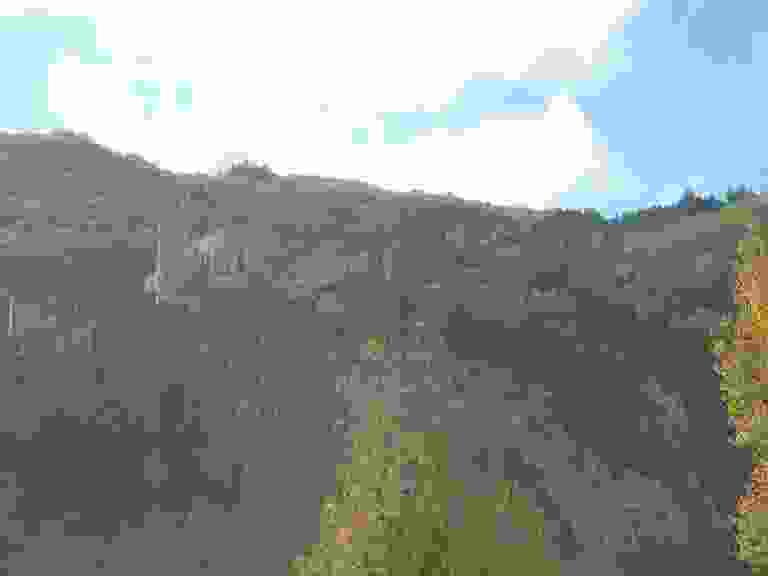
\includegraphics[width=\mywidth]{../wp-content/uploads/2014/11/PB102291.jpg} \end{center}

 Encore quelques km, avant de m'arrêter vers 13h pour pique-niquer au bord de la rivière, au niveau de Sauliac-sur-Célé.
\begin{center} 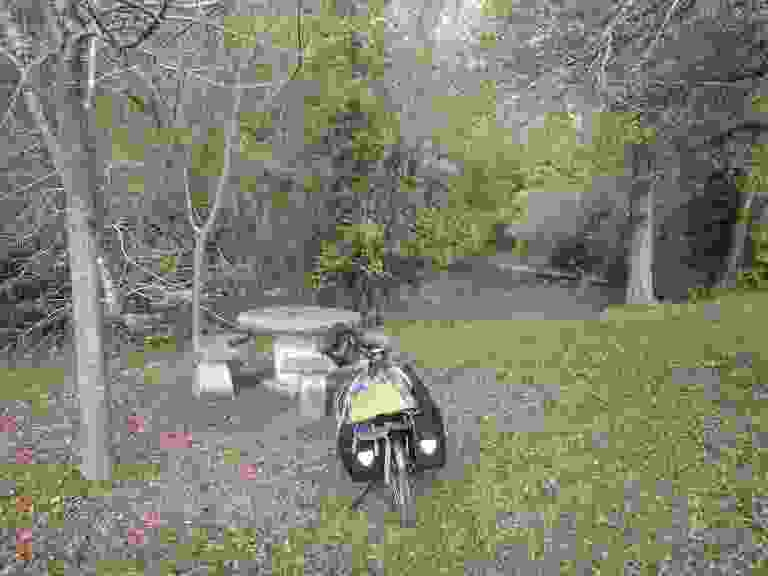
\includegraphics[width=\mywidth]{../wp-content/uploads/2014/11/PB102292.jpg} \end{center}

 Il me reste une quarantaine de km le long de la rivière pour rejoindre Figeac.
 
 Je profite du passage à Espagnac Saint Eulalie pour aller jeter un œil à l'ancien prieuré.
\begin{center} 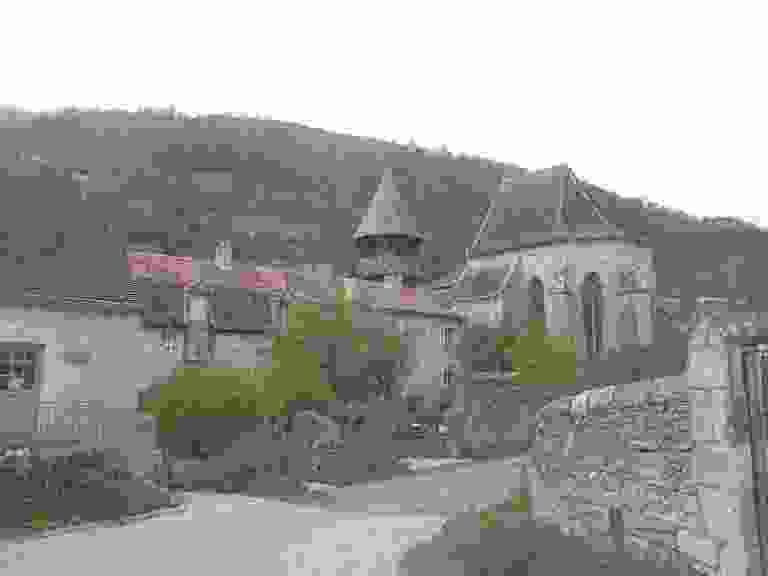
\includegraphics[width=\mywidth]{../wp-content/uploads/2014/11/PB102295.jpg} \end{center}

 J'arrive finalement à Figeac vers 17h, avec 104km dans les jambes.
 
\subsection*{Bilan de la sortie}

 Au niveau du vélo, je suis plutôt rassuré, j'ai de bonnes sensations et une position satisfaisante. Les réglages de vitesses seront à peaufiner car le petit plateau a du mal à passer, peut être qu'un changement de dérailleur avant sera nécessaire.

 Au niveau de la vitesse, je m'aperçois que je ne peux pas rouler très vite. J'ai fait les deux jours à 16km/h de moyenne, sur un parcours vallonné par endroit. Mais même sur les portions plates comme le canal, la moyenne ne dépasse pas 18km/h. Sur les 2 jours, les sensations ont été globalement les mêmes : mise en route le matin assez difficile, un peu de temps pour trouver le rythme. Puis, bonnes sensations en fin de matinée, ça avance bien. Enfin, après-midi plus laborieuse, la vitesse moyenne chute, la fatigue se fait sentir.

 Au niveau de l'endurance, je me rend compte que sur un parcours comme celui-là, il est faisable de faire 100km/jour, mais ça reste une grosse journée, sans trop de pause. Est-ce que l'enchainement de telles distance sur plusieurs jours sera possible ?

 Pour le physique, ça s'est bien passé, pas de douleur particulière à signaler. J'ai roulé la première journée sans cuissard, mais j'ai quand même dû le mettre pour le 2e jour, la selle cuir doit encore avoir besoin d'être rodée avant d'être grand confort comme je l'ai lu un peu partout.

 Concernant le bivouac, je suis très satisfait de la nouvelle tente, légère, simple à monter et pratique. J'avais aussi un nouveau matelas gonflable, un oreiller gonflable et un drap de couchage Thermolite. J'ai passé une bonne nuit, sans avoir froid. C'est plutôt positif car en général, les premières nuits sous tente ne sont pas les meilleures. Enfin, pour un premier camping sauvage seul, j'avais trouvé un bon emplacement pour camper à l'écart de la route, du coup, je n'ai pas été dérangé et ça s'est bien passé.

 Au final, j'ai bien apprécié la sortie. Même les passages sous la pluie sont bien passés. Cependant, pas de rencontre à signaler sur 2 jours, peut-être que la saison et la météo n'étaient pas propices. 

\chapter*{Liste matériel pour voyager en vélo\markboth{Liste matériel pour voyager en vélo}{}}
\section*{21 janvier 2015}
Que va t-il y avoir dans les sacoches pendant le voyage ?

\begin{center} 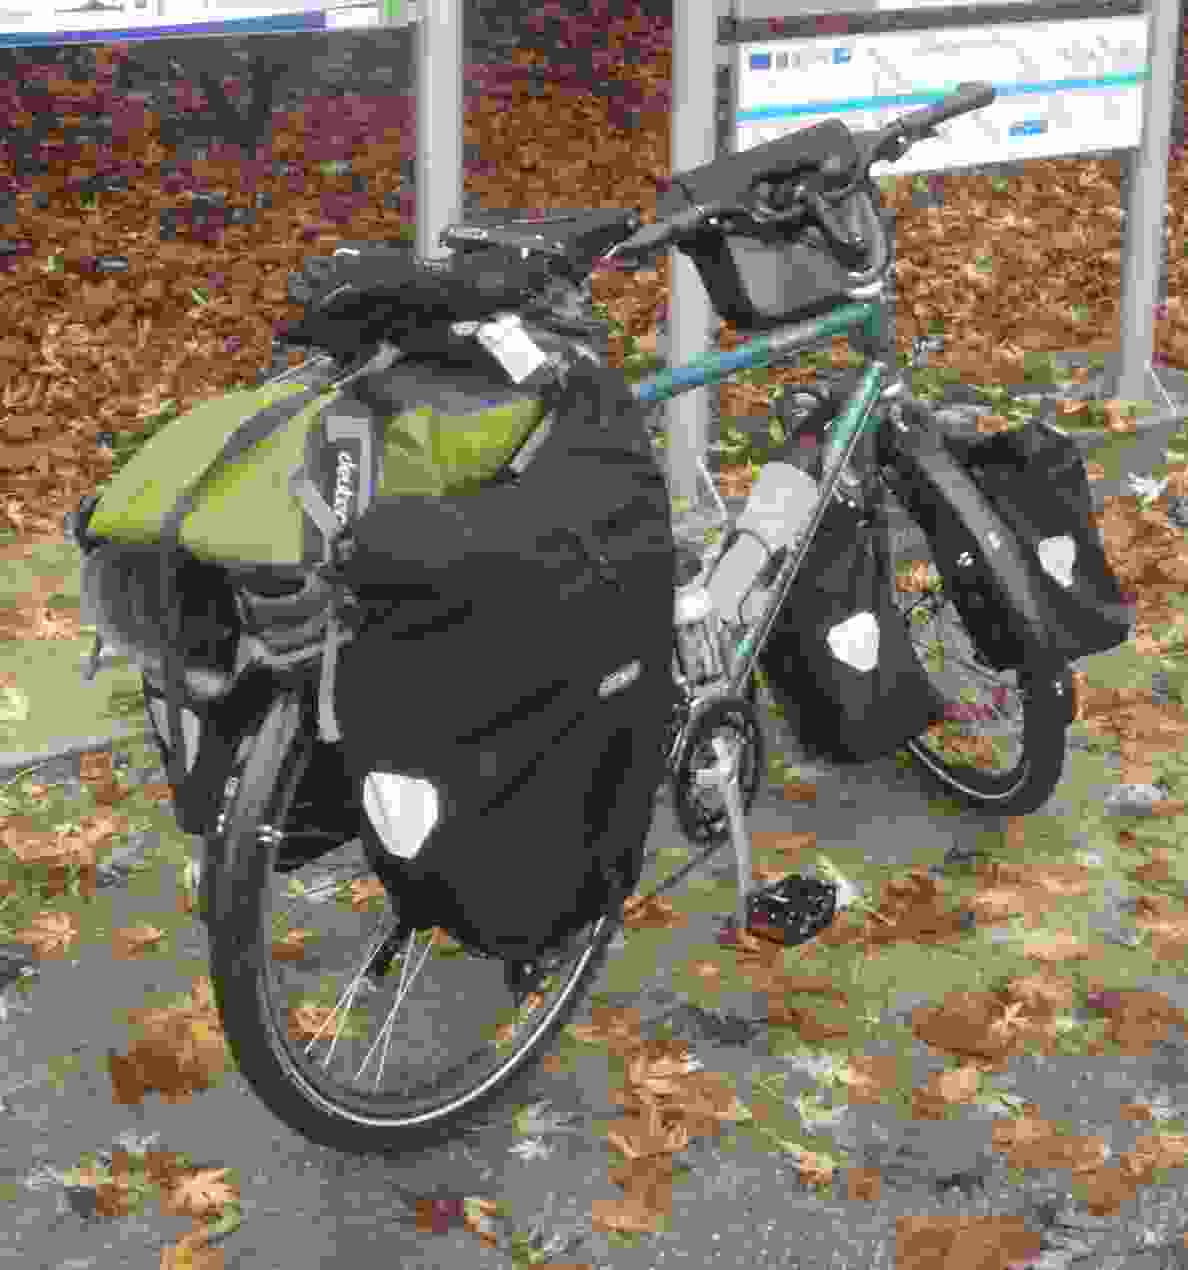
\includegraphics[width=0.68\textwidth]{../wp-content/uploads/2015/01/PB092262.jpg} \end{center}

 Il s'agit de ne rien oublier d'indispensable mais comme toujours il faut optimiser pour ne pas être trop chargé. Cela dit on peut se permettre un peu plus de vêtements en vélo qu'en randonnée où l'on porte tout sur le dos.

\pagebreak
 Voici la liste, tout ça pèse dans les 25kg, hors vélo et eau/nourriture.

 \subsection*{Vélo / Outils / Pièces de rechange}
 \begin{itemize}
 \item Le vélo bien sûr : 16.5 kg à vide
 \item 2 sacoches avant, 2 sacoches arrières et une sacoche de guidon
 \item Éclairage arrière à pile, l'avant se fera à la frontale si besoin
 \item Pompe
 \item Antivol à code
 \item Démonte-pneus
 \item Rustines
 \item Dérive-chaîne
 \item Clé à molette
 \item Clés plates 8/10 et 14/15
 \item Clé à rayons
 \item Pince multifonctions, plate et coupante
 \item Tournevis plat et cruciforme
 \item Jeu de clés Allen
 \item Clés plates fine 13/14/15/16
 \item Graisse pour la chaine
 \item Chiffon et éponge
 \item Patins de freins de rechange
 \item 2 chambres à air de rechange
 \item 4 rayons de rechange
 \item Câbles de rechange pour freins et vitesses
 \item Chaîne de rechange
 \end{itemize}

  \subsection*{ Portage / Bivouac}
 \begin{itemize}
 \item Sac à dos 32L posé sur le porte bagage arrière + sur-sac imperméable
 \item Tente 1 place
 \item Moustiquaire
 \item Matelas + oreiller gonflables
 \item Sac de couchage 0°
 \item Sac à viande thermique
 \item Couverture de survie
 \end{itemize}
 
 \pagebreak
  \subsection*{Vêtements 1ère couche}
 \begin{itemize}
 \item Chaussettes x4
 \item Caleçons x4 + 1 pour dormir
 \item Maillot de bain
 \item Sous-gants
 \item Manchons
 \item Tee-shirts manches courtes x4
 \item Bonnet fin à mettre sous le casque
 \end{itemize}
 
  \subsection*{Vêtements 2ème couche}
 \begin{itemize}
 \item Chaussures trail
 \item Chaussures marche légères
 \item Collant
 \item Pantalons convertibles en short x2
 \item Cuissard vélo
 \item Sous-pull en mérinos
 \item Polaire légère
 \item Veste en duvet
 \end{itemize}

  \subsection*{Vêtements 3ème couche}
 \begin{itemize}
 \item Sur-chaussures étanches
 \item Protection pluie pour les jambes
 \item Veste imperméable Gore Tex
 \item Veste coupe vent légère
 \item Gants Gore Tex
 \item Cache cou
 \item Bonnet
 \item Casque de vélo
 \item Casquette
 \item Lunettes de soleil
 \end{itemize}
 
  \subsection*{Cuisine / Hydratation}
 \begin{itemize}
 \item Couteau suisse
 \item Cuillère
 \item Réchaud gaz + cartouches + feuilles alu pare-vent
 \item Briquet et allumettes
 \item Popote
 \item Éponge
 \item Boites plastiques étanches x2
 \item Gourde 1.5L
 \item Bidons vélo 1L et 0.5L
 \item Filtre à eau céramique + Micropur
 \item Poches à eau 2L et 4L
 \end{itemize}
 
  \subsection*{Hygiène}
 \begin{itemize}
 \item Savon
 \item Shampoing
 \item Lessive à main
 \item Crème solaire
 \item Brosse à dent + dentifrice
 \item Serviettes x2 + gant de toilette
 \item Ciseaux ongles
 \item Mini rasoir électrique
 \item Mouchoirs
 \item Papier toilette
 \end{itemize}
 
  \subsection*{Trousse pharmacie}
 \begin{itemize}
 \item Pansements
 \item Sparadrap
 \item Steri-strip
 \item Bande extensible
 \item Compresses stériles
 \item Tulle gras
 \item Désinfectant
 \item Sérum physiologique
 \item Anti diarrhée
 \item Anti douleur
 \item Pommade infections cutanées
 \item Paracetamol
 \item Chlorure de magnésium
 \item Baume du tigre
 \item Anti moustique corps et vêtements
 \item Pince à tique
 \item Fil + aiguille
 \end{itemize}
 
 \pagebreak
  \subsection*{Électronique / Énergie}
 \begin{itemize}
 \item Appareil photo compact + batterie de rechange
 \item Téléphone
 \item Tablette 7″
 \item Clé USB, carte µSD et SD
 \item Panneau solaire + batterie tampon
 \item Piles de rechange pour frontale, compteur, éclairage
 \end{itemize}
 
  \subsection*{Divers}
 \begin{itemize}
 \item Carnet + stylo
 \item Cartes routières
 \item Boussole à miroir
 \item Chaîne antivol fine
 \item Scotch
 \item Colle forte
 \item Frontale
 \item Papiers, photocopies, passeport...
 \item Argent
 \item Sacs poubelles + Ziploc
 \end{itemize}

\chapter*{Départ J-1\markboth{Départ J-1}{}}
\section*{7 février 2015}
C'est demain le grand départ à 18h55 de l'aéroport de Toulouse et non pas 6h55 comme je l'avais dit à tout le monde. Petite confusion de ma part entre l'heure AM et l'heure PM. \newline
 Ensuite ça sera une escale à Madrid puis 13h45 de vol jusqu'à Santiago du Chili. Si les sacoches, le vélo et moi arrivont entiers à Santiago, un dernier vol me conduira à Puerto Montt vers le sud du Chili dans la région des lacs. \newline
 Prêt à embarquer \newline
 Le vélo dans son carton à vélo : \newline
 \newline
\centerline{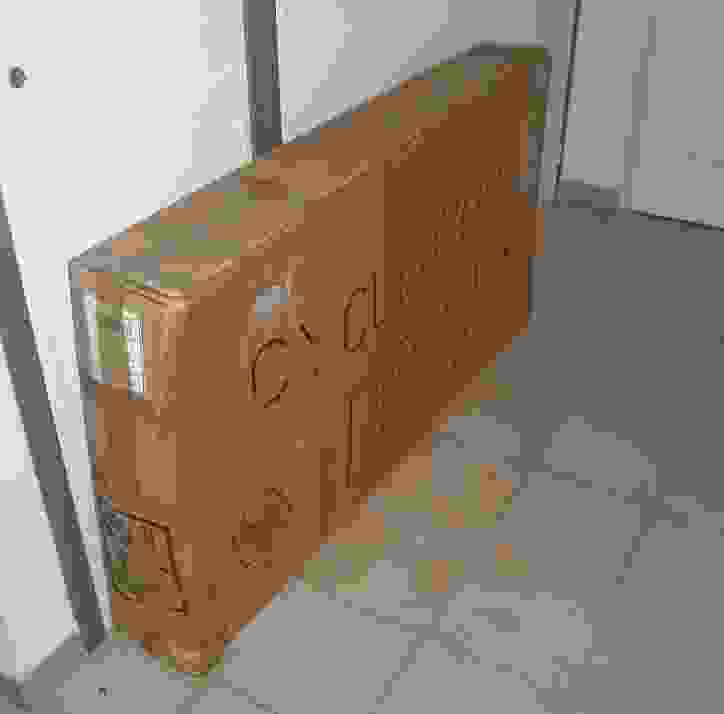
\includegraphics[width=\mywidth]{../wp-content/uploads/2015/02/Carton-velo.jpg} } 
 \newline
 Les sacoches prêtes pour la soute et le sac à dos qui passera en cabine avec un peu de chance : \newline
 
\chapter*{Ça commence : vers l’île de Chiloe\markboth{Ça commence : vers l’île de Chiloe}{}}
\section*{13 février 2015}
Arrivée à Santiago du Chili avec la mauvaise surprise de voir le carton du vélo ouvert et une pédale manquante. Je demande au personnel des bagages s'ils peuvent la retrouver mais sans succès. 

 Au passage c'était une bonne idée d'apprendre un peu d'espagnol parce que quasiment personne ne parle anglais, même à l'aéroport.
\begin{center} 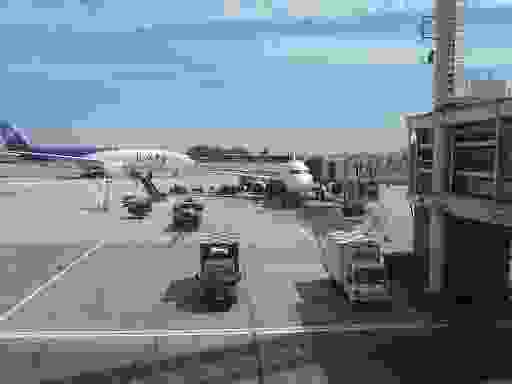
\includegraphics[width=\mywidth]{../wp-content/uploads/2015/02/P2092025.jpg} \end{center}

 Dernier vol entre Santiago et Puerto Montt : je cherche un moyen pour rejoindre le centre ville comme je ne peux pas monter le vélo. 
 Pas de chance le seul distributeur de l'aéroport est vide et les CB ne sont pas acceptées pour le bus ou les taxis. 
Heureusement une touriste allemande me propose de partager un taxi. Et au moment de charger le vélo dans le taxi, la pédale que je croyais perdue tombe du carton, ouf ! 

 Le taxi nous pose à l'hôtel de l'allemande et je vois que la personne chez qui je devais rester en couchsurfing ne peut pas m'accueillir finalement. Du coup je reste à l'hôtel pour cette première nuit.
\begin{center} 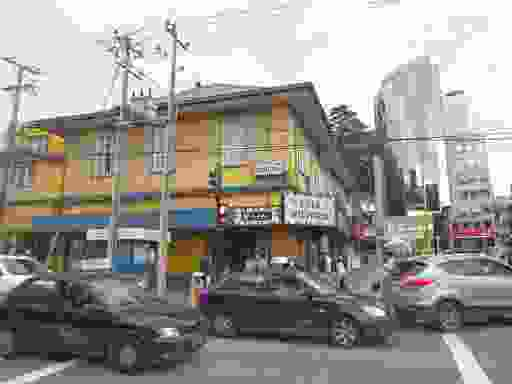
\includegraphics[width=\mywidthreduced]{../wp-content/uploads/2015/02/P2092027.jpg} \end{center}

 Puerto Montt, le bord de mer :
\begin{center} 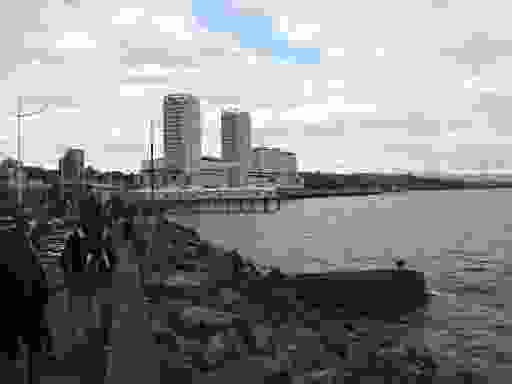
\includegraphics[width=\mywidthreduced]{../wp-content/uploads/2015/02/P2092029.jpg} \end{center}

 Le lendemain, 60 km d'autoroute vers l'île de Chiloe :
\begin{center} 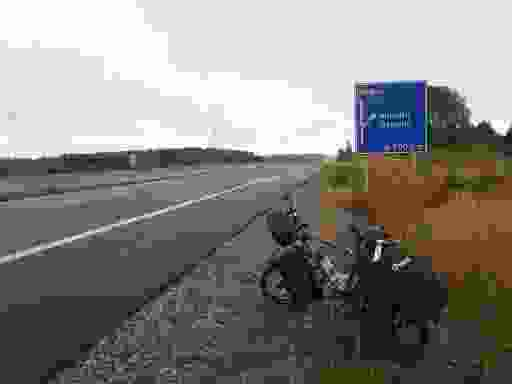
\includegraphics[width=\mywidth]{../wp-content/uploads/2015/02/P2102037.jpg} \end{center}

 Puis traversée en ferry :
\begin{center} 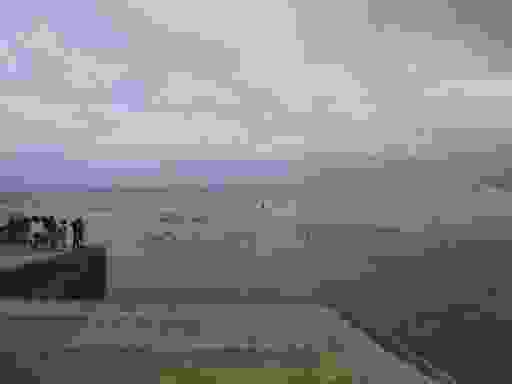
\includegraphics[width=\mywidth]{../wp-content/uploads/2015/02/P2102039.jpg} \end{center}
\vspace{-\topsep}

\pagebreak
~
\begin{center} 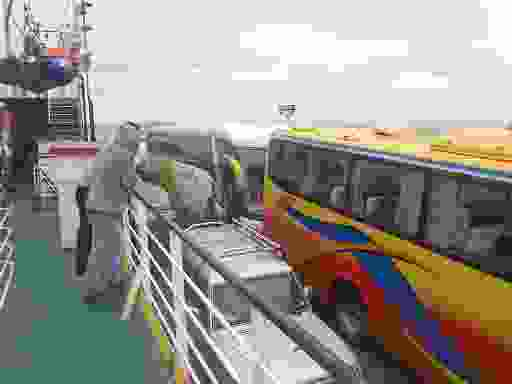
\includegraphics[width=\mywidth]{../wp-content/uploads/2015/02/P2102041.jpg} \end{center}
~
\begin{center} 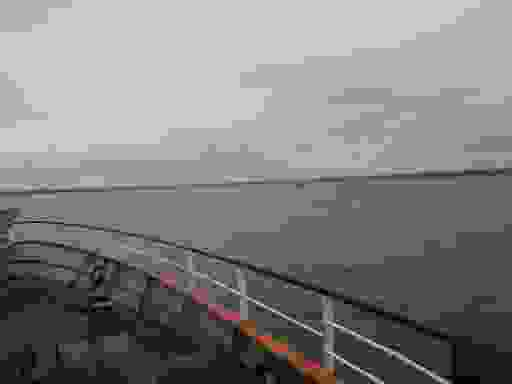
\includegraphics[width=\mywidth]{../wp-content/uploads/2015/02/P2102043.jpg} \end{center}
\vspace{-\topsep}

\pagebreak
 Petit village de Chacao :\\
\begin{center} 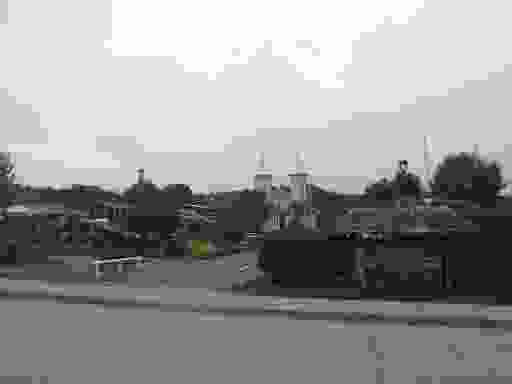
\includegraphics[width=\mywidth]{../wp-content/uploads/2015/02/P2102045.jpg} \end{center}
~\\

~
\begin{center} 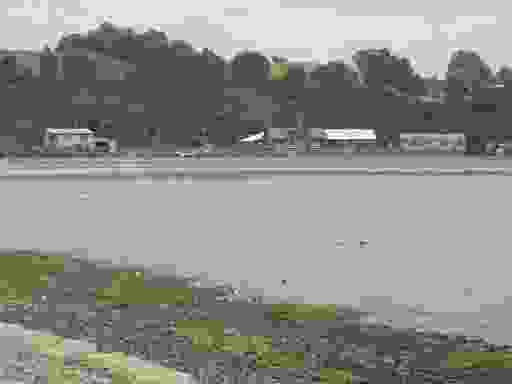
\includegraphics[width=\mywidth]{../wp-content/uploads/2015/02/P2102047.jpg} \end{center}
\vspace{-\topsep}

\pagebreak
 Première nuit de camping, pas simple de trouver un endroit car presque tout est clôturé sur l'île, j'ai du demander pour m'installer. 
\begin{center} 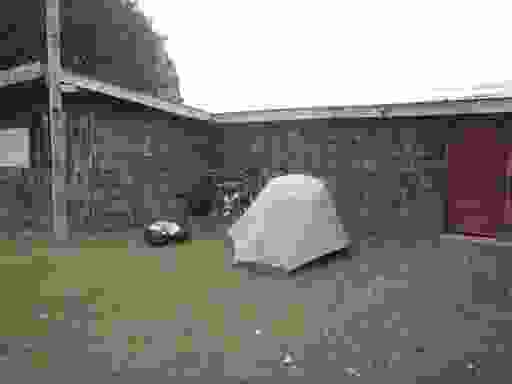
\includegraphics[width=\mywidth]{../wp-content/uploads/2015/02/P2112048.jpg} \end{center}

 25km de route vers la ville d'Ancud où je rencontre 3 cyclistes, 2 français et 1 espagnol, l'occasion de recevoir quelques conseils.

 Le port d'Ancud :
\begin{center} 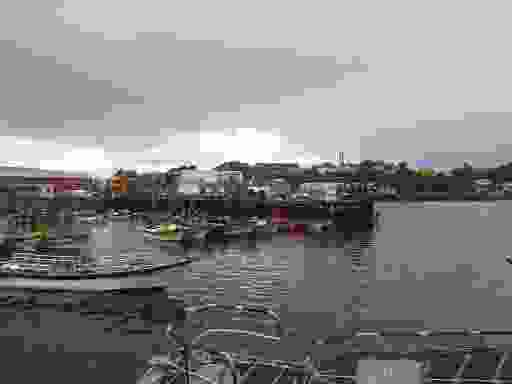
\includegraphics[width=\mywidth]{../wp-content/uploads/2015/02/P2122061.jpg} \end{center}
\vspace{-\topsep}

\pagebreak
~
\vspace{-3mm}
\begin{center} 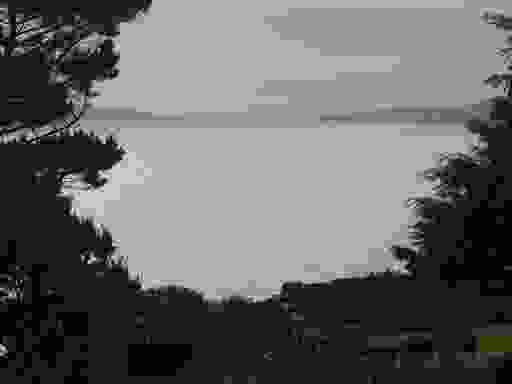
\includegraphics[width=\mywidth]{../wp-content/uploads/2015/02/P2122063.jpg} \end{center}

 Camping avec douche chaude :
\begin{center} 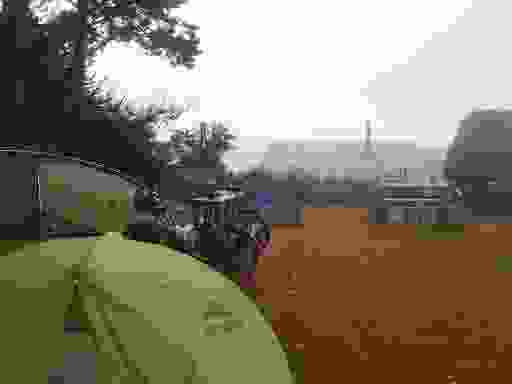
\includegraphics[width=\mywidth]{../wp-content/uploads/2015/02/P2122057.jpg} \end{center}
\vspace{-\topsep}

\pagebreak
Spécialité chilienne : pomme de terre frite avec une garniture viande / olives.
\begin{center} 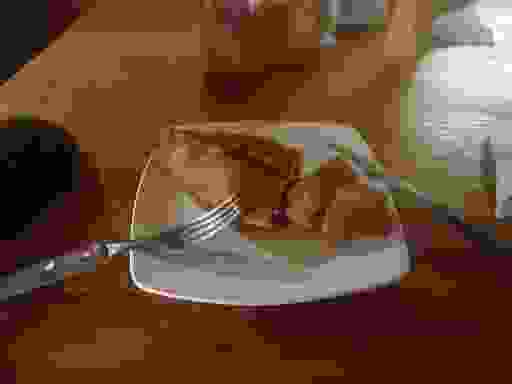
\includegraphics[width=\mywidth]{../wp-content/uploads/2015/02/P2122060.jpg} \end{center}
\chapter{Chiloe : journée à Puñihuil}
\section*{18 février 2015}
Enfin une journée qui s´annonce sous le soleil ! \newline
 \newline
\centerline{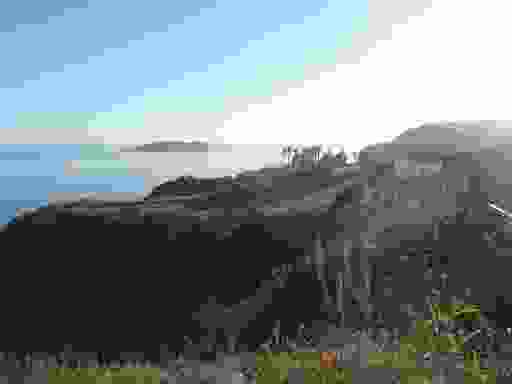
\includegraphics[width=\mywidth]{../wp-content/uploads/2015/02/P2122067.jpg} } 
 \newline
 30km de belle route le long de la côte pour aller à la Pinguineria de Puñihuil. \newline
 \newline
\centerline{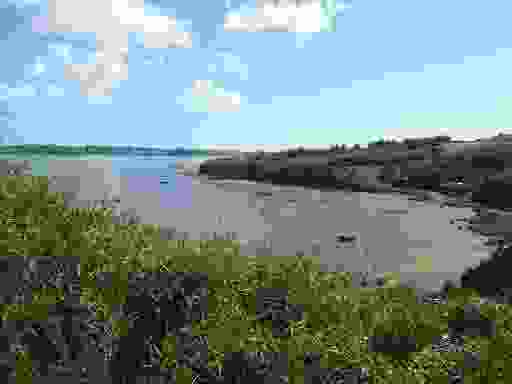
\includegraphics[width=\mywidth]{../wp-content/uploads/2015/02/P2122070.jpg} } 
 \newline
\centerline{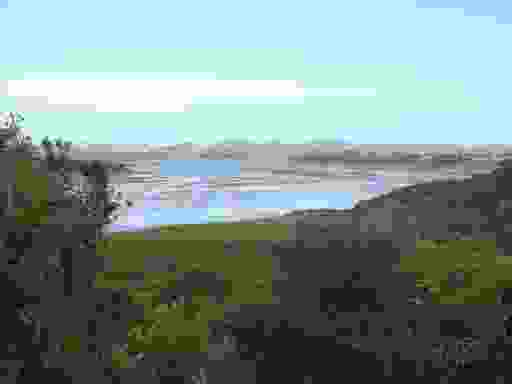
\includegraphics[width=\mywidth]{../wp-content/uploads/2015/02/P2122072.jpg} } 
 \newline
\centerline{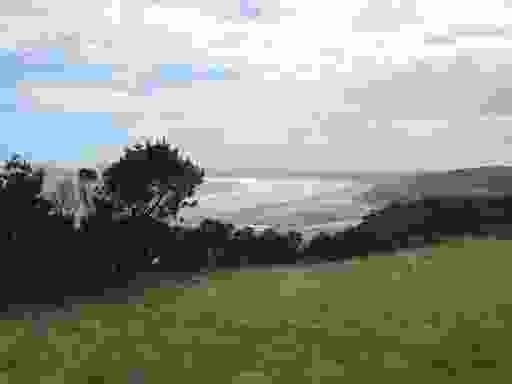
\includegraphics[width=\mywidth]{../wp-content/uploads/2015/02/P2122073.jpg} } 
 \newline
\centerline{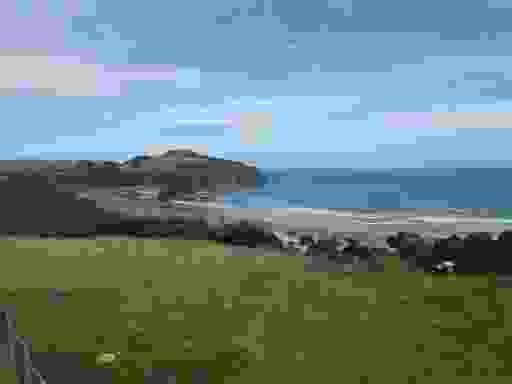
\includegraphics[width=\mywidth]{../wp-content/uploads/2015/02/P2122074.jpg} } 
 \newline
\centerline{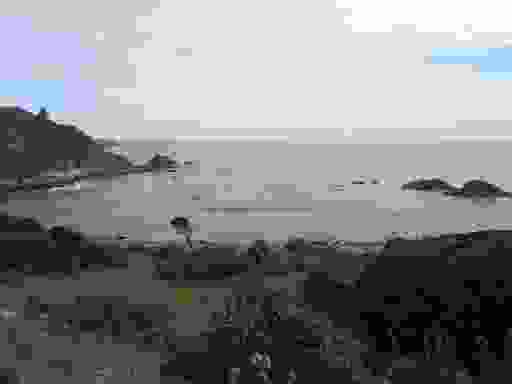
\includegraphics[width=\mywidth]{../wp-content/uploads/2015/02/P2122075.jpg} } 
 Rencontre avec Carlo, un cycliste italien \newline
 \newline
\centerline{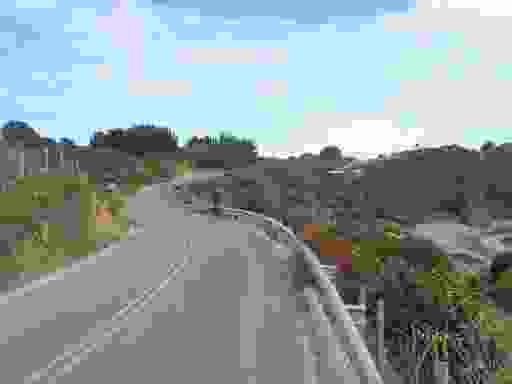
\includegraphics[width=\mywidth]{../wp-content/uploads/2015/02/P2122077.jpg} } 
 Tour en bateau depuis la plage \newline
 \newline
\centerline{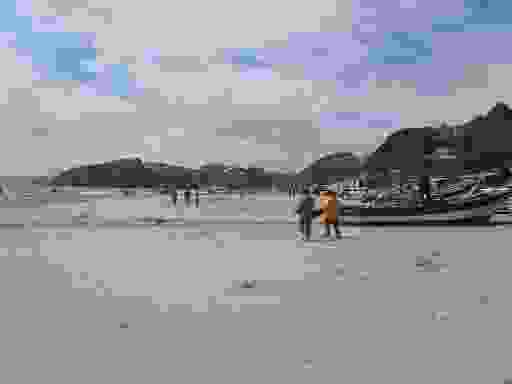
\includegraphics[width=\mywidth]{../wp-content/uploads/2015/02/P2122079.jpg} } 
 \newline
\centerline{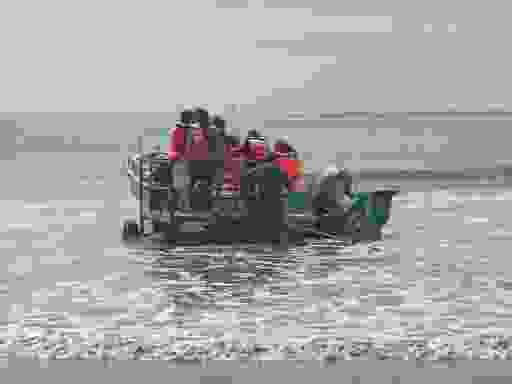
\includegraphics[width=\mywidth]{../wp-content/uploads/2015/02/P2122080.jpg} } 
 Il y a 2 espèces différentes de pingouins sur l´ìle. \newline
\centerline{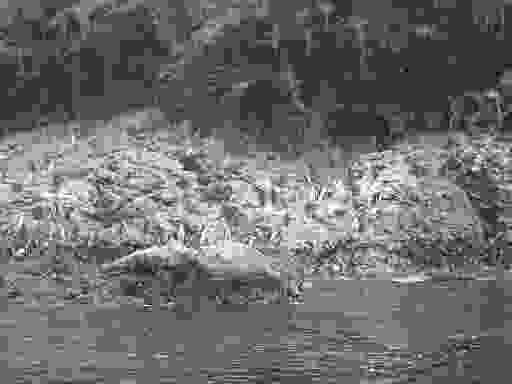
\includegraphics[width=\mywidth]{../wp-content/uploads/2015/02/P2122084.jpg} } 
 \newline
\centerline{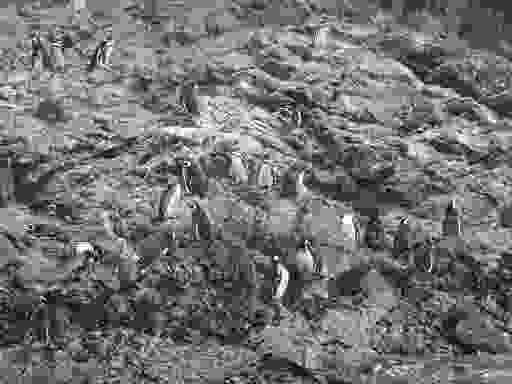
\includegraphics[width=\mywidth]{../wp-content/uploads/2015/02/P2122087.jpg} } 
 \newline
\centerline{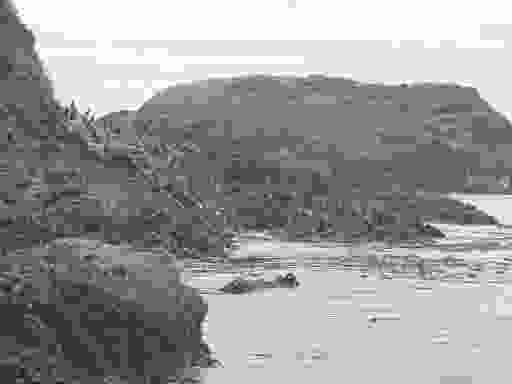
\includegraphics[width=\mywidth]{../wp-content/uploads/2015/02/P2122088.jpg} } 
 Des pelicans \newline
\centerline{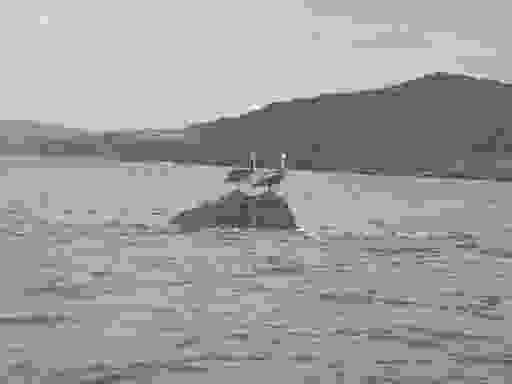
\includegraphics[width=\mywidth]{../wp-content/uploads/2015/02/P2122094.jpg} } 
 Je reprend la route avec Carlo sur un chemin en gravier qui enchaîne montées et descentes raides. \newline
 Trop difficile pour mon vélo : le filetage qui fixe les pignons au moyeu est mort et je ne peux plus avancer car je pédale dans le vide. \newline
 \newline
\centerline{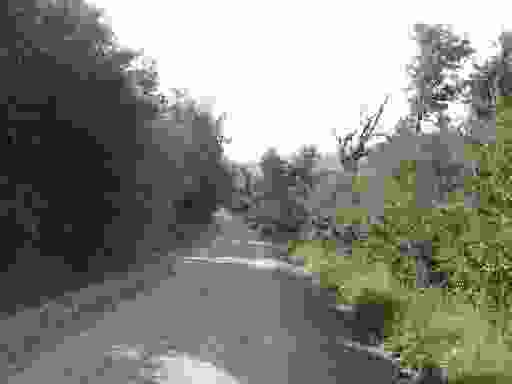
\includegraphics[width=\mywidth]{../wp-content/uploads/2015/02/P2122095.jpg} } 
 Demi tour pour rejoindre la route à pied : par chance un pick up s'arrête et accepte de me déposer à Ancud. \newline
 Changement du moyeu dans un magasin de vélo, le technicien est efficace il a démonté, remonté tous les rayons de la roue arrière et dévoilé la roue en à peine 1h et demie. \newline
 Du coup je retourne au même camping que la veille et je recroise Javier et Jonathan, 2 voyageurs à vélo que j´avais déjà rencontrés. \newline
 \newline
\centerline{\includegraphics[width=\mywidth]{../wp-content/uploads/2015/02/P2132096.jpg} } 
 \newline

\newpage
 

\chapter*{Traversée de Chiloe\markboth{Traversée de Chiloe}{}}
\section*{22 février 2015}
6 jours pour traverser l'île de Chiloe en vélo du nord au sud.

 Je commence à descendre par la route principale ce qui permet d'avancer bien car la route est goudronnée et avec des montées raisonnables.
\begin{center} \includegraphics[width=\mywidth]{../wp-content/uploads/2015/02/P2132099.jpg} \end{center}
\vspace{-\topsep}

\pagebreak
 Suite en direction de la côte à l'est, on aperçoit quelques sommets de la cordillère des Andes au loin.
\begin{center} \includegraphics[width=\mywidth]{../wp-content/uploads/2015/02/P2132098.jpg} \end{center}
\begin{center} \includegraphics[width=\mywidth]{../wp-content/uploads/2015/02/P2142124.jpg} \end{center}
\vspace{-\topsep}
\vspace{-3mm}

\pagebreak
 Visite d'un petit îlot :
\begin{center} \includegraphics[width=\mywidth]{../wp-content/uploads/2015/02/P2142106.jpg} \end{center}
\begin{center} \includegraphics[width=\mywidth]{../wp-content/uploads/2015/02/P2142108.jpg} \end{center}
\vspace{-\topsep}
\vspace{-3.25mm}

\pagebreak
~
\begin{center} \includegraphics[width=\mywidth]{../wp-content/uploads/2015/02/P2142109.jpg} \end{center}
\begin{center} \includegraphics[width=\mywidth]{../wp-content/uploads/2015/02/P2142110.jpg} \end{center}
\vspace{-\topsep}
\vspace{-3.25mm}

\pagebreak
 Passage par une partie de la route des églises de Chiloe, plusieurs d'entre elles sont au patrimoine de l'Unesco.

 \'Eglise de Colo, 3km de piste aller-retour super raide pour y arriver, ça se mérite !

\begin{center} \includegraphics[width=\mywidth]{../wp-content/uploads/2015/02/P2142113.jpg} \end{center}

 \'Eglise de Castro :
\begin{center} \includegraphics[width=\mywidth]{../wp-content/uploads/2015/02/P2152142.jpg} \end{center}

 \'Eglise de Nercon :
\begin{center} \includegraphics[width=\mywidth]{../wp-content/uploads/2015/02/P2152150.jpg} \end{center}

 Après je ne les ai pas toutes vues, il y en a une vingtaine au total.

 Passage par une cascade sympathique :
\begin{center} \includegraphics[width=\mywidth]{../wp-content/uploads/2015/02/P2142119.jpg} \end{center}

 Juste avant d´arriver à Castro, la capitale de l´île je me fais rattraper par Jérémy que j´avais croisé à Ancud. Il voyage en vélo depuis 2 ans et demi, il a déjà parcouru la route entre terre de feu et le Canada. Il est revenu dans le sud pour faire quelques endroits qu´il ne connait pas encore !
\begin{center} \includegraphics[width=\mywidth]{../wp-content/uploads/2015/02/P2152135.jpg} \end{center}

 Puisque nous allons tous les 2 vers le sud de l´île, nous continuons la route ensemble.

 Castro et ses maisons sur pilotis :
\begin{center} \includegraphics[width=\mywidth]{../wp-content/uploads/2015/02/P2152133.jpg} \end{center}
\vspace{-\topsep}

\pagebreak
~\\
\begin{center} \includegraphics[width=\mywidth]{../wp-content/uploads/2015/02/P2152146.jpg} \end{center}

~

 Je fais bien du vélo ici :\\
\begin{center} \includegraphics[width=\mywidth]{../wp-content/uploads/2015/02/P2152141.jpg} \end{center}
\vspace{-\topsep}

\pagebreak
 Petite fête locale avec de la musique et des spécialités culinaires :
\begin{center} \includegraphics[width=\mywidth]{../wp-content/uploads/2015/02/P2152151.jpg} \end{center}

 Après Castro, nous repartons vers la côte Pacifique et le parc national de Chiloe.

 La route longe un beau lac, l'occasion de se rafraîchir.
\begin{center} \includegraphics[width=\mywidth]{../wp-content/uploads/2015/02/P2162156.jpg} \end{center}
\vspace{-\topsep}

\pagebreak
~
\begin{center} \includegraphics[width=\mywidth]{../wp-content/uploads/2015/02/P2162158.jpg} \end{center}
~\\

~
\begin{center} \includegraphics[width=\mywidth]{../wp-content/uploads/2015/02/P2162161.jpg} \end{center}
\vspace{-\topsep}

\pagebreak
 Plage immense au bord du pacifique :
\begin{center} \includegraphics[width=\mywidth]{../wp-content/uploads/2015/02/P2162164.jpg} \end{center}

 Bivouac à quelques mètres de la plage :
\begin{center} \includegraphics[width=\mywidth]{../wp-content/uploads/2015/02/P2172173.jpg} \end{center}
\vspace{-\topsep}

\pagebreak
~
\begin{center} \includegraphics[width=\mywidth]{../wp-content/uploads/2015/02/P2172175.jpg} \end{center}
~
\begin{center} \includegraphics[width=\mywidth]{../wp-content/uploads/2015/02/P2172180.jpg} \end{center}
\vspace{-\topsep}

\pagebreak
 Balade dans le parc national qui contient des forêts très denses et à la végétation particulière :
\begin{center} \includegraphics[width=\mywidth]{../wp-content/uploads/2015/02/P2162167.jpg} \end{center}
\begin{center} \includegraphics[width=\mywidth]{../wp-content/uploads/2015/02/P2162169.jpg} \end{center}
\vspace{-\topsep}
\vspace{-3mm}

\pagebreak
  Dernier bivouac avant de quitter Chiloe :
\begin{center} \includegraphics[width=\mywidth]{../wp-content/uploads/2015/02/P2172189.jpg} \end{center}

 Et encore quelques spécialités locales sur la route.

 Les empanadas, il y en a partout avec différentes garnitures, viande, fromage, légumes...
\begin{center} \includegraphics[width=\mywidth]{../wp-content/uploads/2015/02/P2142116.jpg} \end{center}
\vspace{-\topsep}

\pagebreak
 Le Curanto, typique de Chiloe, coquillages, saucisse, porc, pomme de terre et fèves, le tout cuit dans des pierres chaudes.
 \vfill
 \begin{center} \includegraphics[width=\mywidth]{../wp-content/uploads/2015/02/P2152152.jpg} \end{center}

\vfill
 Le Mote con Huesilla, boisson sucrée avec une pêche et des grains de blé au fond.
 \vfill
\begin{center} \includegraphics[width=\mywidth]{../wp-content/uploads/2015/02/P2172183.jpg} \end{center}
\vspace{-\topsep}
\vspace{-0.75mm}
\chapter*{La Carretera Austral\markboth{La Carretera Austral}{}}
\section*{28 février 2015}
Retour sur le continent chilien après l'île de Chiloe pour emprunter une partie de la Carretera Austral, superbe route qui traverse la Patagonie chilienne sur plus de 1000km. 

 J'avais prévu d'en faire environ 700km mais j'ai du changer mes plans à cause du ferry que je n'ai pas pu avoir plus tôt. 

 Le ferry m'a donc amené à Puerto Raul Marin Balmaceda, un tout petit village où pas grand monde ne va.
\begin{center} \includegraphics[width=\mywidth]{../wp-content/uploads/2015/02/P2192198.jpg} \end{center}
\vspace{-\topsep}

\pagebreak
~\\
\begin{center} \includegraphics[width=\mywidth]{../wp-content/uploads/2015/02/P2192200.jpg} \end{center}
\begin{center} \includegraphics[width=\mywidth]{../wp-content/uploads/2015/02/P2192201.jpg} \end{center}
\vspace{-\topsep}
\vspace{-3mm}

\pagebreak
70km de piste pour rejoindre la Carretera Austral, le long de la belle rivière Palena.
\begin{center} \includegraphics[width=\mywidth]{../wp-content/uploads/2015/02/P2192214.jpg} \end{center}
\begin{center} \includegraphics[width=\mywidth]{../wp-content/uploads/2015/02/P2192216.jpg} \end{center}
\vspace{-\topsep}
\vspace{-3mm}

\pagebreak
~
\begin{center} \includegraphics[width=\mywidth]{../wp-content/uploads/2015/02/P2192220.jpg} \end{center}
\begin{center} \includegraphics[width=\mywidth]{../wp-content/uploads/2015/02/P2192227.jpg} \end{center}
\vspace{-\topsep}
\vspace{-3.25mm}

\pagebreak
 Superbe bivouac au bord de l'eau.
\begin{center} \includegraphics[width=\mywidth]{../wp-content/uploads/2015/02/P2202230.jpg} \end{center}
\begin{center} \includegraphics[width=\mywidth]{../wp-content/uploads/2015/02/P2202236.jpg} \end{center}
\begin{center} \includegraphics[width=\mywidth]{../wp-content/uploads/2015/02/P2202242.jpg} \end{center}
\begin{center} \includegraphics[width=\mywidth]{../wp-content/uploads/2015/02/P22022451.jpg} \end{center}
\begin{center} \includegraphics[width=\mywidth]{../wp-content/uploads/2015/02/P2202234.jpg} \end{center}

Première étape sur la Carretera entre La Junta et Villa Santa Lucia.
\begin{center} \includegraphics[width=\mywidth]{../wp-content/uploads/2015/02/P2202251.jpg} \end{center}
\begin{center} \includegraphics[width=\mywidth]{../wp-content/uploads/2015/02/P2202258.jpg} \end{center}
\begin{center} \includegraphics[width=\textwidth]{../wp-content/uploads/2015/02/P2202254.jpg} \end{center}
\begin{center} \includegraphics[width=\mywidth]{../wp-content/uploads/2015/02/P2202253.jpg} \end{center}
\begin{center} \includegraphics[width=\mywidth]{../wp-content/uploads/2015/02/P2202260.jpg} \end{center}
\begin{center} \includegraphics[width=\mywidth]{../wp-content/uploads/2015/02/P2202262.jpg} \end{center}
\vspace{-\topsep}
\vspace{-8.5mm}

\pagebreak
~
\begin{center} \includegraphics[width=\mywidth]{../wp-content/uploads/2015/02/P2202263.jpg} \end{center}
\begin{center} \includegraphics[width=\mywidth]{../wp-content/uploads/2015/02/P2202264.jpg} \end{center}
\vspace{-\topsep}
\vspace{-3.25mm}

\pagebreak
Le passage de la piste à la route qui fait plaisir !
\begin{center} \includegraphics[width=\mywidth]{../wp-content/uploads/2015/02/P2202265.jpg} \end{center}
\begin{center} \includegraphics[width=\mywidth]{../wp-content/uploads/2015/02/P2202266.jpg} \end{center}
\vspace{-\topsep}
\vspace{-3.25mm}

\pagebreak
~
\begin{center} \includegraphics[width=\mywidth]{../wp-content/uploads/2015/02/P2202267.jpg} \end{center}
~
\begin{center} \includegraphics[width=\mywidth]{../wp-content/uploads/2015/02/P2202269.jpg} \end{center}
\vspace{-\topsep}

\pagebreak
Pas mal d'autres voyageurs à vélo dans les campings.
\begin{center} \includegraphics[width=\mywidth]{../wp-content/uploads/2015/02/P2212275.jpg} \end{center}

Deuxième étape jusqu'à Chaiten.
\begin{center} \includegraphics[width=\mywidth]{../wp-content/uploads/2015/02/P2212277.jpg} \end{center}
\begin{center} \includegraphics[width=\mywidth]{../wp-content/uploads/2015/02/P2212280.jpg} \end{center}
\begin{center} \includegraphics[width=\mywidth]{../wp-content/uploads/2015/02/P2212281.jpg} \end{center}
\begin{center} \includegraphics[width=\mywidth]{../wp-content/uploads/2015/02/P2212283.jpg} \end{center}
\begin{center} \includegraphics[width=\mywidth]{../wp-content/uploads/2015/02/P2212284.jpg} \end{center}
\begin{center} \includegraphics[width=\mywidth]{../wp-content/uploads/2015/02/P2212285.jpg} \end{center}
\begin{center} \includegraphics[width=\mywidth]{../wp-content/uploads/2015/02/P2212286.jpg} \end{center}
\begin{center} \includegraphics[width=\mywidth]{../wp-content/uploads/2015/02/P2212288.jpg} \end{center}
\vfill
\begin{center} \includegraphics[width=\mywidth]{../wp-content/uploads/2015/02/P2212290.jpg} \end{center}
\vspace{-\topsep}
\vspace{-0.75mm}

\pagebreak
Petit détour pour profiter des thermes d'eau chaude.
\begin{center} \includegraphics[width=\mywidth]{../wp-content/uploads/2015/02/P2212292.jpg} \end{center}
~\\
\begin{center} \includegraphics[width=\mywidth]{../wp-content/uploads/2015/02/P2212294.jpg} \end{center}
\vspace{-\topsep}
\pagebreak
~
\begin{center} \includegraphics[width=\mywidth]{../wp-content/uploads/2015/02/P2222297.jpg} \end{center}

\`A Chaiten, je suis invité par une famille chilienne rencontrée à une fête locale sur la route.
\begin{center} \includegraphics[width=\mywidth]{../wp-content/uploads/2015/02/P2232319.jpg} \end{center}
\vspace{-\topsep}

\pagebreak
~\\
\begin{center} \includegraphics[width=\mywidth]{../wp-content/uploads/2015/02/P2232314.jpg} \end{center}
\begin{center} \includegraphics[width=\mywidth]{../wp-content/uploads/2015/02/P2232317.jpg} \end{center}
\vspace{-\topsep}
\vspace{-3mm}

\pagebreak
Du coup, je reste 2 jours ce qui me permet de faire l'ascension du volcan Chaiten, 962m de haut et entré en éruption en 2008.
\begin{center} \includegraphics[width=\mywidth]{../wp-content/uploads/2015/02/P2222302.jpg} \end{center}
\begin{center} \includegraphics[width=\mywidth]{../wp-content/uploads/2015/02/P2222305.jpg} \end{center}
\begin{center} \includegraphics[width=\mywidth]{../wp-content/uploads/2015/02/P2222310.jpg} \end{center}
\begin{center} \includegraphics[width=\mywidth]{../wp-content/uploads/2015/02/P2222311.jpg} \end{center}
\begin{center} \includegraphics[width=\mywidth]{../wp-content/uploads/2015/02/P2222312.jpg} \end{center}

Je continue direction Caleta Gonzalo, à l'intérieur du parc Pumalin.
\begin{center} \includegraphics[width=\mywidth]{../wp-content/uploads/2015/02/P2222300.jpg} \end{center}
\begin{center} \includegraphics[width=\mywidth]{../wp-content/uploads/2015/02/P2232321.jpg} \end{center}
\begin{center} \includegraphics[width=\mywidth]{../wp-content/uploads/2015/02/P2232323.jpg} \end{center}
\begin{center} \includegraphics[width=\mywidth]{../wp-content/uploads/2015/02/P2232326.jpg} \end{center}
\vfill
\begin{center} \includegraphics[width=\mywidth]{../wp-content/uploads/2015/02/P2232330.jpg} \end{center}
\vspace{-\topsep}
\vspace{-0.75mm}

\pagebreak
 Journée sur le ferry, encore magnifique entre fjords, montagnes et glaciers.
\begin{center} \includegraphics[width=\mywidth]{../wp-content/uploads/2015/02/P2242333.jpg} \end{center}
\begin{center} \includegraphics[width=\mywidth]{../wp-content/uploads/2015/02/P2242335.jpg} \end{center}
\vspace{-\topsep}
\vspace{-3mm}

\pagebreak
~\\
\begin{center} \includegraphics[width=\mywidth]{../wp-content/uploads/2015/02/P2242338.jpg} \end{center}
\begin{center} \includegraphics[width=\mywidth]{../wp-content/uploads/2015/02/P2242342.jpg} \end{center}
\begin{center} \includegraphics[width=\mywidth]{../wp-content/uploads/2015/02/P2242345.jpg} \end{center}
\begin{center} \includegraphics[width=\mywidth]{../wp-content/uploads/2015/02/P2242347.jpg} \end{center}
\begin{center} \includegraphics[width=\mywidth]{../wp-content/uploads/2015/02/P2242348.jpg} \end{center}
\begin{center} \includegraphics[width=\mywidth]{../wp-content/uploads/2015/02/P2242351.jpg} \end{center}
\begin{center} \includegraphics[width=\mywidth]{../wp-content/uploads/2015/02/P2242354.jpg} \end{center}
\begin{center} \includegraphics[width=\mywidth]{../wp-content/uploads/2015/02/P2242355.jpg} \end{center}
\begin{center} \includegraphics[width=\mywidth]{../wp-content/uploads/2015/02/P2242358.jpg} \end{center}
\begin{center} \includegraphics[width=\mywidth]{../wp-content/uploads/2015/02/P2242359.jpg} \end{center}
\begin{center} \includegraphics[width=\mywidth]{../wp-content/uploads/2015/02/P2242363.jpg} \end{center}
\begin{center} \includegraphics[width=\mywidth]{../wp-content/uploads/2015/02/P2242364.jpg} \end{center}
\begin{center} \includegraphics[width=\mywidth]{../wp-content/uploads/2015/02/P2242366.jpg} \end{center}
\vfill
\begin{center} \includegraphics[width=\mywidth]{../wp-content/uploads/2015/02/P2252370.jpg} \end{center}
\vspace{-\topsep}
\vspace{-0.75mm}

\pagebreak
Sur le bateau, j'ai rencontré un couple de français qui m'a proposé de m'avancer en direction de Puerto Montt. Du coup je suis arrivé plus rapidement en évitant au passage une partie de piste en travaux qui aurait été galère.

 J'en ai profité pour visiter le marché de poissons d'Angelmo.
\begin{center} \includegraphics[width=\mywidth]{../wp-content/uploads/2015/02/P2252373.jpg} \end{center}
\begin{center} \includegraphics[width=\mywidth]{../wp-content/uploads/2015/02/P2252372.jpg} \end{center}
\vspace{-\topsep}
\vspace{-1.25mm}

\pagebreak
  Saumon au beurre dans un des nombreux restaurants du marché.
\begin{center} \includegraphics[width=\mywidth]{../wp-content/uploads/2015/02/P2252376.jpg} \end{center}
\begin{center} \includegraphics[width=\mywidth]{../wp-content/uploads/2015/02/P2252375.jpg} \end{center}
\vspace{-\topsep}
\vspace{-3.25mm}

\pagebreak
  Passage par Puerto Varas au bord du lac Llanquihue, petite ville avec une architecture d'influence allemande.
\begin{center} \includegraphics[width=\mywidth]{../wp-content/uploads/2015/02/P2252379.jpg} \end{center}

Belle route le long du lac avec piste cyclable.
\begin{center} \includegraphics[width=\mywidth]{../wp-content/uploads/2015/02/P2252386.jpg} \end{center}
\vspace{-\topsep}
\pagebreak
~\\
\begin{center} \includegraphics[width=\mywidth]{../wp-content/uploads/2015/02/P2252387.jpg} \end{center}

 Vues sur le volcan Osorno.
\begin{center} \includegraphics[width=\mywidth]{../wp-content/uploads/2015/02/P2252385.jpg} \end{center}
\vspace{-\topsep}

\pagebreak
~
\begin{center} \includegraphics[width=\mywidth]{../wp-content/uploads/2015/02/P2262390.jpg} \end{center}
\begin{center} \includegraphics[width=\mywidth]{../wp-content/uploads/2015/02/P2262395.jpg} \end{center}
\vspace{-\topsep}
\vspace{-3.25mm}

\pagebreak
Arrivée le lendemain aux chutes de Petrohué.
\begin{center} \includegraphics[width=\mywidth]{../wp-content/uploads/2015/02/P2262401.jpg} \end{center}
\begin{center} \includegraphics[width=\mywidth]{../wp-content/uploads/2015/02/P2262403.jpg} \end{center}
\vspace{-\topsep}
\vspace{-3.25mm}

\pagebreak
 C'est terminé pour le sud du Chili, prochaine étape Santiago puis l'île de Pâques.
\begin{center} \includegraphics[width=\mywidth]{../wp-content/uploads/2015/02/P2282417.jpg} \end{center}

\chapter{Santiago du Chili}
\section*{11 mars 2015}
Au retour de l'île de Pâques, je retrouve le vélo chez Nelson qui m'héberge 2 nuits de plus. \newline
\centerline{\includegraphics[width=\mywidth]{../wp-content/uploads/2015/03/P3012432-1024x768.jpg} } 
 Santiago se prête assez bien au vélo, il y a quelques pistes cyclables et des parcs agréables. \newline
\centerline{\includegraphics[width=\mywidth]{../wp-content/uploads/2015/03/P3062599.jpg} } 
 \newline
\centerline{\includegraphics[width=\mywidth]{../wp-content/uploads/2015/03/P3062598-1024x768.jpg} } 
\newline
\centerline{\includegraphics[width=\mywidth]{../wp-content/uploads/2015/03/P3052566-1024x768.jpg} } 
\newline
\centerline{\includegraphics[width=\mywidth]{../wp-content/uploads/2015/03/P3062617-1024x768.jpg} } 
 Rue piétonne dans le centre.\newline
\centerline{\includegraphics[width=\mywidth]{../wp-content/uploads/2015/03/P3062630-1024x768.jpg} } 
 Le Palacio de la Moneda, le palais présidentiel. \newline
\centerline{\includegraphics[width=\mywidth]{../wp-content/uploads/2015/03/P2282423-1024x768.jpg} } 
 \newline
\centerline{\includegraphics[width=\mywidth]{../wp-content/uploads/2015/03/P2282424-1024x768.jpg} } 
 \newline
\centerline{\includegraphics[width=\mywidth]{../wp-content/uploads/2015/03/P3062612-1024x768.jpg} } 
La colline Santa Lucia qui donne une vue intéressante sur le centre ville. \newline
\centerline{\includegraphics[width=\mywidth]{../wp-content/uploads/2015/03/P3052571-1024x768.jpg} } 
 \newline
\centerline{\includegraphics[width=\mywidth]{../wp-content/uploads/2015/03/P3052573-1024x768.jpg} } 
 \newline
\centerline{\includegraphics[width=\mywidth]{../wp-content/uploads/2015/03/P3052578-1024x768.jpg} } 
 \newline
\centerline{\includegraphics[width=\mywidth]{../wp-content/uploads/2015/03/P3052580-1024x768.jpg} } 
Le Mercado Central, marché aux poissons. \newline
\centerline{\includegraphics[width=\mywidth]{../wp-content/uploads/2015/03/P3052583-1024x768.jpg} } 
 \newline
\centerline{\includegraphics[width=\mywidth]{../wp-content/uploads/2015/03/P3052584-1024x768.jpg} } 
J'ai goûté à la Paila Marina, une soupe de fruits de mer. \newline
\centerline{\includegraphics[width=\mywidth]{../wp-content/uploads/2015/03/P3052587-1024x768.jpg} } 
La colline San Cristobal, immense parc avec une vue encore plus panoramique sur Santiago. On distingue même la cordillère des Andes au loin. \newline
\centerline{\includegraphics[width=\mywidth]{../wp-content/uploads/2015/03/P3052588-1024x768.jpg} } 
 \newline
\centerline{\includegraphics[width=\mywidth]{../wp-content/uploads/2015/03/P3052589-1024x768.jpg} } 
 \newline
\centerline{\includegraphics[width=\mywidth]{../wp-content/uploads/2015/03/P3052590-1024x768.jpg} } 
 \newline
\centerline{\includegraphics[width=\mywidth]{../wp-content/uploads/2015/03/P3052591-1024x768.jpg} } 
 \newline
\centerline{\includegraphics[width=\mywidth]{../wp-content/uploads/2015/03/P3052592-1024x768.jpg} } 
A côté de la grande tour, le Costanera Center, immense centre commercial. \newline
\centerline{\includegraphics[width=\mywidth]{../wp-content/uploads/2015/03/P2282428-1024x768.jpg} } 
 \newline
\centerline{\includegraphics[width=\mywidth]{../wp-content/uploads/2015/03/P2282431-1024x768.jpg} } 
 Le Terremoto, cocktailtypique à base de vin blanc, jus de fruit, liqueur et glace. Très bon ! \newline
\centerline{\includegraphics[width=\mywidth]{../wp-content/uploads/2015/03/P3062608-117x300.jpg} } 
 Dernier jour à Santiago dans un hostel qui donne directement sur la place d'armes, l'idéal ! \newline
\centerline{\includegraphics[width=\mywidth]{../wp-content/uploads/2015/03/P3062616-1024x768.jpg} } 
 \newline
\centerline{\includegraphics[width=\mywidth]{../wp-content/uploads/2015/03/P3062606-1024x768.jpg} } 
 \newline
\centerline{\includegraphics[width=\mywidth]{../wp-content/uploads/2015/03/P3072632-1024x768.jpg} } 
  La route vers Valparaiso \newline
 Après 3 jours de visite de Santiago, je remonte sur le vélo direction Valparaiso. Presque 125km par une autoroute plus ou moins agréable en vélo. La route passait par 2 tunnels interdits au vélos, heureusement le stop marche bien au Chili j'ai traversé sans trop de difficulté. \newline
 Passage par la région de Casablanca au milieu des vignes. \newline
\centerline{\includegraphics[width=\mywidth]{../wp-content/uploads/2015/03/P3072634-1024x768.jpg} } 
 \newline
\centerline{\includegraphics[width=\mywidth]{../wp-content/uploads/2015/03/P3072635-1024x768.jpg} } 
 \newline
\centerline{\includegraphics[width=\mywidth]{../wp-content/uploads/2015/03/P3072636-1024x768.jpg} } 
  Je me suis arrêté pour une petite dégustation : un syrah 2013\newline
\centerline{\includegraphics[width=\mywidth]{../wp-content/uploads/2015/03/P3072637-1024x768.jpg} } 
 \newline
\centerline{\includegraphics[width=\mywidth]{../wp-content/uploads/2015/03/P3072642-1024x768.jpg} } 
 \newline
\centerline{\includegraphics[width=\mywidth]{../wp-content/uploads/2015/03/P3082646-1024x768.jpg} } 
Avant d´arriver à Valparaiso, la Reserva Nacional Lago Peñuelas,réserve de faune et de flore autour d´un lac. \newline
\centerline{\includegraphics[width=\mywidth]{../wp-content/uploads/2015/03/P3082661-1024x768.jpg} } 
 \newline
\centerline{\includegraphics[width=\mywidth]{../wp-content/uploads/2015/03/P3082659-1024x768.jpg} } 
 Il y avait même quelques lamas. \newline
\centerline{\includegraphics[width=\mywidth]{../wp-content/uploads/2015/03/P3082653-1024x768.jpg} } 
 \newline
\centerline{\includegraphics[width=\mywidth]{../wp-content/uploads/2015/03/P3082656-1024x768.jpg} } 
 \newline

\newpage
 

\chapter*{Valparaiso\markboth{Valparaiso}{}}
\section*{14 mars 2015}
Après Santiago, nouvelle étape \og ville \fg\ avec Valparaiso et juste à côté Viña del Mar.

 \subsection*{Valparaiso}
 La ville est dans la brume tous les matins.
\begin{center} \includegraphics[width=\mywidth]{../wp-content/uploads/2015/03/P3092690-1024x768.jpg} \end{center}
\begin{center} \includegraphics[width=\mywidth]{../wp-content/uploads/2015/03/P30926731-1024x768.jpg} \end{center}

Puis l'après-midi ça se dégage.
\begin{center} \includegraphics[width=\mywidth]{../wp-content/uploads/2015/03/P3112753-1024x768.jpg} \end{center}
\begin{center} \includegraphics[width=\mywidth]{../wp-content/uploads/2015/03/P3112755-1024x768.jpg} \end{center}
\begin{center} \includegraphics[width=\mywidth]{../wp-content/uploads/2015/03/P3112756-1024x768.jpg} \end{center}
\begin{center} \includegraphics[width=\mywidth]{../wp-content/uploads/2015/03/P3112748-1024x768.jpg} \end{center}
\begin{center} \includegraphics[width=\mywidth]{../wp-content/uploads/2015/03/P3092710-1024x768.jpg} \end{center}
\begin{center} \includegraphics[width=\mywidth]{../wp-content/uploads/2015/03/P3092695-1024x768.jpg} \end{center}

La ville est très colorée avec de nombreuses fresques sur les murs. Il y a aussi des coins assez sales.
\begin{center} \includegraphics[width=\mywidth]{../wp-content/uploads/2015/03/P3092675-1024x768.jpg} \end{center}
\begin{center} \includegraphics[height=\mywidth]{../wp-content/uploads/2015/03/P3092677-768x1024.jpg} \end{center}
\begin{center} \includegraphics[width=\mywidth]{../wp-content/uploads/2015/03/P3092708-1024x768.jpg} \end{center}
\begin{center} \includegraphics[width=\mywidth]{../wp-content/uploads/2015/03/P3112757-1024x768.jpg} \end{center}
\begin{center} \includegraphics[width=\mywidth]{../wp-content/uploads/2015/03/P3112744-1024x768.jpg} \end{center}
\begin{center} \includegraphics[width=\mywidth]{../wp-content/uploads/2015/03/P3092686-1024x768.jpg} \end{center}

 La Plaza Sotomayor en plein centre.
\begin{center} \includegraphics[width=\mywidth]{../wp-content/uploads/2015/03/P3082665-1024x768.jpg} \end{center}
\begin{center} \includegraphics[width=\mywidth]{../wp-content/uploads/2015/03/P3082666-1024x768.jpg} \end{center}

 De multiples petits funiculaires permettent d'accéder aux hauteurs de la ville.
\begin{center} \includegraphics[width=\mywidth]{../wp-content/uploads/2015/03/P3092679-1024x768.jpg} \end{center}
\vspace{-\topsep}

\pagebreak
\begin{center} \includegraphics[width=\mywidth]{../wp-content/uploads/2015/03/P3092682-1024x768.jpg} \end{center}
~\\

\begin{center} \includegraphics[width=\mywidth]{../wp-content/uploads/2015/03/P3092693-1024x768.jpg} \end{center}
\vspace{-\topsep}
\vspace{-3mm}

\pagebreak
Le marché aux fruits.
\begin{center} \includegraphics[width=\mywidth]{../wp-content/uploads/2015/03/P3082664-1024x768.jpg} \end{center}

Ils font du bon boulot !
\begin{center} \includegraphics[width=\mywidth]{../wp-content/uploads/2015/03/P3092698-1024x768.jpg} \end{center}
\vspace{-\topsep}

\pagebreak
 L'hostel où j'ai logé à Valparaiso, tenu par un français et aussi avec beaucoup de clients français.
\begin{center} \includegraphics[width=\mywidth]{../wp-content/uploads/2015/03/P3092668-1024x768.jpg} \end{center}

 Un soir, un chilien a préparé un superbe plat de fruits de mer, poulet et pommes de terre. Le tout cuit au feu de bois, un régal !
\begin{center} \includegraphics[width=\mywidth]{../wp-content/uploads/2015/03/P3112743-1024x768.jpg} \end{center}
\begin{center} \includegraphics[width=\mywidth]{../wp-content/uploads/2015/03/P3112742-1024x768.jpg} \end{center}

 \subsection*{Viña del Mar}
 \`A peine à 10km de Valparaiso mais avec une ambiance totalement différente, ville balnéaire très propre avec de belles plages et des grands immeubles face à la mer.
\begin{center} \includegraphics[width=\mywidth]{../wp-content/uploads/2015/03/P3102721-1024x768.jpg} \end{center}
\begin{center} \includegraphics[width=\mywidth]{../wp-content/uploads/2015/03/P3102726-1024x768.jpg} \end{center}
\begin{center} \includegraphics[width=\mywidth]{../wp-content/uploads/2015/03/P3102728-1024x768.jpg} \end{center}
\begin{center} \includegraphics[width=\mywidth]{../wp-content/uploads/2015/03/P31027291-1024x768.jpg} \end{center}
\begin{center} \includegraphics[width=\mywidth]{../wp-content/uploads/2015/03/P3102731-1024x768.jpg} \end{center}
\begin{center} \includegraphics[width=\mywidth]{../wp-content/uploads/2015/03/P3102732-1024x768.jpg} \end{center}
\begin{center} \includegraphics[width=\mywidth]{../wp-content/uploads/2015/03/P3102735-1024x768.jpg} \end{center}
\begin{center} \includegraphics[width=\mywidth]{../wp-content/uploads/2015/03/P3102738-1024x768.jpg} \end{center}
\begin{center} \includegraphics[width=\mywidth]{../wp-content/uploads/2015/03/P3102739-1024x768.jpg} \end{center}
\begin{center} \includegraphics[width=\mywidth]{../wp-content/uploads/2015/03/P3102741-1024x768.jpg} \end{center}

\chapter{Geysers d’El Tatio}
\section*{20 mars 2015}
Après Valparaiso plusieurs possibilités : continuer en vélo ou prendre un bus vers le nord. J'ai décidé d'aller directement à San Pedro de Atacama pour pouvoir bien profiter de toute la région nord du Chili, altiplano bolivien et sud du Pérou. \newline
 Je vais donc à la gare de bus de Valparaiso à 23h pour un trajet qui doit durer plus de 24h. Malheureusement je suis tombé sur un chauffeur un peu borné qui a refusé d'embarquer le vélo. Résultat une nuit de plus à Valparaiso et un départ le lendemain midi mais vers la ville de Calama à 100km de San Pedro. \newline
 \newline
\centerline{\includegraphics[height=90mm]{../wp-content/uploads/2015/03/P3122760-1024x768.jpg} } 
 \newline
 En remontant le vélo en arrivant, je vois que la roue arrière tourne difficilement : cette fois c'est le cône de roulement qui est usé, heureusement j'ai trouvé un magasin pour changer la pièce rapidement. Les réparateurs chiliens sont décidément efficaces ! \newline
 Calama, dans la région des mines de cuivres. \newline
 \newline
\centerline{\includegraphics[height=90mm]{../wp-content/uploads/2015/03/P3132768-1024x768.jpg} } 
 \newline
 Au lieu de prendre la route directe vers San Pedro, je profite d'être à Calama pour faire un détour par les geysers d'El Tatio. \newline
 C'est parti pour environ 5 jours en quasi autonomie, vélo bien chargé en nourriture et en eau, un bon test pour la suite en Bolivie. \newline
 La première partie traverse le désert. \newline
 \newline
\centerline{\includegraphics[height=90mm]{../wp-content/uploads/2015/03/P3142773-1024x768.jpg} } 
 \newline
\centerline{\includegraphics[height=90mm]{../wp-content/uploads/2015/03/P3142776-1024x768.jpg} } 
\newline
\centerline{\includegraphics[height=90mm]{../wp-content/uploads/2015/03/P3142782-1024x768.jpg} } 
Je passe par le village de Chiu Chiu. \newline
 \newline
\centerline{\includegraphics[height=90mm]{../wp-content/uploads/2015/03/P3142777-1024x768.jpg} } 
 \newline
\centerline{\includegraphics[height=90mm]{../wp-content/uploads/2015/03/P3142779-1024x768.jpg} } 
Un petit lac au milieu du désert. \newline
 \newline
\centerline{\includegraphics[height=90mm]{../wp-content/uploads/2015/03/P3142786-1024x768.jpg} } 
Puis ça commence à monter jusqu´au premier bivouac : je ne sais pas à quelle altitude mais les effets se font un peu sentir. \newline
 \newline
\centerline{\includegraphics[height=90mm]{../wp-content/uploads/2015/03/P3142794-1024x768.jpg} } 
 \newline
\centerline{\includegraphics[height=90mm]{../wp-content/uploads/2015/03/P3152798-1024x768.jpg} } 
 \newline
 Deuxième jour, ça continue à monter sérieusement. \newline
 Mes réserves d'eau sont un peu juste, je dois faire un aller retour de 8km vers un village pour me ravitailler. \newline
 \newline
\centerline{\includegraphics[height=90mm]{../wp-content/uploads/2015/03/P3142793-1024x768.jpg} } 
 \newline
 \newline
\centerline{\includegraphics[height=90mm]{../wp-content/uploads/2015/03/P3152810-1024x768.jpg} } 
 \newline
 Ça valait quand même le coup, le village de Caspana est très joli. \newline
 \newline
\centerline{\includegraphics[height=90mm]{../wp-content/uploads/2015/03/P3152814-1024x768.jpg} } 
 \newline
\centerline{\includegraphics[height=90mm]{../wp-content/uploads/2015/03/P3152818-1024x768.jpg} } 
 \newline
\centerline{\includegraphics[height=90mm]{../wp-content/uploads/2015/03/P3152819-1024x768.jpg} } 
 \newline
\centerline{\includegraphics[height=90mm]{../wp-content/uploads/2015/03/P3152821-1024x768.jpg} } 
 \newline
\centerline{\includegraphics[height=90mm]{../wp-content/uploads/2015/03/P3152820-1024x768.jpg} } 
 \newline
 Je reprends la route qui continue à bien monter. Je croise quelques animaux. \newline
 \newline
\centerline{\includegraphics[height=90mm]{../wp-content/uploads/2015/03/P3152827-1024x768.jpg} } 
 \newline
 \newline
\centerline{\includegraphics[height=90mm]{../wp-content/uploads/2015/03/P3152826-1024x768.jpg} } 
 \newline
 \newline
\centerline{\includegraphics[height=90mm]{../wp-content/uploads/2015/03/P3152832-1024x768.jpg} } 
 \newline
 Vers 16h le temps se couvre et l´orage n´est pas loin. J´hésite à continuer mais il commence à pleuvoir, je me dépêche de poser la tente où je peux. \newline
 \newline
\centerline{\includegraphics[height=90mm]{../wp-content/uploads/2015/03/P3162833-1024x768.jpg} } 
 \newline
 Le 3e jour débute sous un beau ciel bleu et des paysages magnifiques. \newline
 \newline
\centerline{\includegraphics[height=90mm]{../wp-content/uploads/2015/03/P3162835-1024x768.jpg} } 
 \newline
 \newline
\centerline{\includegraphics[height=90mm]{../wp-content/uploads/2015/03/P3162836-1024x768.jpg} } 
 \newline
 \newline
\centerline{\includegraphics[height=90mm]{../wp-content/uploads/2015/03/P3162837-1024x768.jpg} } 
 \newline
 \newline
\centerline{\includegraphics[height=90mm]{../wp-content/uploads/2015/03/P31628401-1024x768.jpg} } 
 \newline
 \newline
\centerline{\includegraphics[height=90mm]{../wp-content/uploads/2015/03/P31628411-1024x768.jpg} } 
 \newline
 \newline
\centerline{\includegraphics[height=90mm]{../wp-content/uploads/2015/03/P31628441-1024x768.jpg} } 
 \newline
 \newline
\centerline{\includegraphics[height=90mm]{../wp-content/uploads/2015/03/P3162848-1024x768.jpg} } 
 \newline
 \newline
\centerline{\includegraphics[height=90mm]{../wp-content/uploads/2015/03/P31628491-1024x768.jpg} } 
Mais encore une fois ça se couvre dès midi et je roule pour essayer d'atteindre les geysers rapidement. \newline
 \newline
\centerline{\includegraphics[height=90mm]{../wp-content/uploads/2015/03/P3162854-1024x768.jpg} } 
 \newline
 \newline
\centerline{\includegraphics[height=90mm]{../wp-content/uploads/2015/03/P3162856-1024x768.jpg} } 
 \newline
 Par chance la fin n'est pas trop difficile et j'arrive assez rapidement au refuge d'El Tatio à 4200m. \newline
 Les gardiens sont un peu surpris de voir arriver un vélo, surtout que les touristes ne viennent que le matin et dès 11h il n'y a plus personne. \newline
 \newline
\centerline{\includegraphics[height=90mm]{../wp-content/uploads/2015/03/P3162862-1024x768.jpg} } 
 \newline
 J'ai le champ de geysers pour moi tout seul l'après midi. \newline
 \newline
\centerline{\includegraphics[height=90mm]{../wp-content/uploads/2015/03/P3162868-1024x768.jpg} } 
 \newline
 \newline
\centerline{\includegraphics[height=90mm]{../wp-content/uploads/2015/03/P3162874-1024x768.jpg} } 
 \newline
 \newline
\centerline{\includegraphics[height=90mm]{../wp-content/uploads/2015/03/P3162878-1024x768.jpg} } 
 \newline
 \newline
\centerline{\includegraphics[height=90mm]{../wp-content/uploads/2015/03/P3162879-1024x768.jpg} } 
 \newline
 \newline
\centerline{\includegraphics[height=90mm]{../wp-content/uploads/2015/03/P3162885-1024x768.jpg} } 
 \newline
 \newline
\centerline{\includegraphics[height=90mm]{../wp-content/uploads/2015/03/P3162886-1024x768.jpg} } 
 \newline
 \newline
\centerline{\includegraphics[height=90mm]{../wp-content/uploads/2015/03/P3162890-1024x768.jpg} } 
 \newline
 \newline
\centerline{\includegraphics[height=90mm]{../wp-content/uploads/2015/03/P3162892-1024x768.jpg} } 
 \newline
 Ainsi que la piscine d'eau chaude ! \newline
 \newline
\centerline{\includegraphics[height=90mm]{../wp-content/uploads/2015/03/P3162884-1024x768.jpg} } 
 \newline
 Le lendemain matin un petit tour aux geysers, la lumière est différente mais il y a monde cette fois. \newline
 \newline
\centerline{\includegraphics[height=90mm]{../wp-content/uploads/2015/03/P3172894-1024x768.jpg} } 
 \newline
 \newline
\centerline{\includegraphics[height=90mm]{../wp-content/uploads/2015/03/P3172897-1024x768.jpg} } 
 \newline
 \newline
\centerline{\includegraphics[height=90mm]{../wp-content/uploads/2015/03/P3172898-1024x768.jpg} } 
 \newline
 \newline
\centerline{\includegraphics[height=90mm]{../wp-content/uploads/2015/03/P3172900-1024x768.jpg} } 
 \newline
 \newline
\centerline{\includegraphics[height=90mm]{../wp-content/uploads/2015/03/P3172902-1024x768.jpg} } 
 \newline
 \newline
\centerline{\includegraphics[height=90mm]{../wp-content/uploads/2015/03/P3172903-1024x768.jpg} } 
 \newline
 Puis c´est la descente :90km de 4200m à 2500m pour rejoindre San Pedro de Atacama. \newline
 \newline
\centerline{\includegraphics[height=90mm]{../wp-content/uploads/2015/03/P3172904-1024x768.jpg} } 
 \newline
 \newline
\centerline{\includegraphics[height=90mm]{../wp-content/uploads/2015/03/P3172905-1024x768.jpg} } 
 \newline
 \newline
\centerline{\includegraphics[height=90mm]{../wp-content/uploads/2015/03/P3172908-1024x768.jpg} } 
 \newline
 Je croise régulièrement des vigognes.\newline
\centerline{\includegraphics[height=90mm]{../wp-content/uploads/2015/03/P3172909-1024x768.jpg} } 
 \newline
 \newline
\centerline{\includegraphics[height=90mm]{../wp-content/uploads/2015/03/P3172911-1024x768.jpg} } 
 \newline
 \newline
\centerline{\includegraphics[height=90mm]{../wp-content/uploads/2015/03/P3172912-1024x768.jpg} } 
 \newline
 \newline
\centerline{\includegraphics[height=90mm]{../wp-content/uploads/2015/03/P3172919-1024x768.jpg} } 
 \newline
 \newline
\centerline{\includegraphics[height=90mm]{../wp-content/uploads/2015/03/P3172922-1024x768.jpg} } 
 \newline
 Le désert d´Atacama au loin. \newline
 \newline
\centerline{\includegraphics[height=90mm]{../wp-content/uploads/2015/03/P3172925-1024x768.jpg} } 
 \newline
 A San Pedro je suis hébergé en Warmshowers chez Carlos, en compagnie d'un couple de voyageurs à vélo français Frédéric et Lucie. Quelques jours de repos bien sympatiques. \newline
 \newline
\centerline{\includegraphics[height=90mm]{../wp-content/uploads/2015/03/P3172927-1024x768.jpg} } 
 \newline
 \newline
\centerline{\includegraphics[height=90mm]{../wp-content/uploads/2015/03/P31829291-1024x768.jpg} } 
J´attaque bientôt le sud de la Bolivie, une région plutôt isolée, le prochain article ne sera pas pour tout de suite. \newline
 Et merci à tous pour les commentaires, ça m´encourage bien! \newline
  \newline

\newpage
 

\chapter*{L’île de Pâques\markboth{L’île de Pâques}{}}
\section*{8 mars 2015}
Petite entorse au règlement du voyage, je suis parti 3 jours sur l'île de Pâques sans le vélo. Il est resté à Santiago chez Nelson, un chilien qui m'a hébergé en Couchsurfing.

 Camping au bord de l'océan dans la petite ville d'Hanga Roa, la seule de l'île.
\begin{center} \includegraphics[width=\mywidth]{../wp-content/uploads/2015/03/P3012436-1024x768.jpg} \end{center}

\pagebreak
Petite balade au bord de l'eau et les premiers Moais sont là.
\begin{center} \includegraphics[width=\mywidth]{../wp-content/uploads/2015/03/P3032529-1024x768.jpg} \end{center}
\begin{center} \includegraphics[width=\mywidth]{../wp-content/uploads/2015/03/P3012439-1024x768.jpg} \end{center}
\begin{center} \includegraphics[width=\mywidth]{../wp-content/uploads/2015/03/P3012444-1024x768.jpg} \end{center}
\begin{center} \includegraphics[width=\mywidth]{../wp-content/uploads/2015/03/P3012445-1024x768.jpg} \end{center}
\begin{center} \includegraphics[width=\mywidth]{../wp-content/uploads/2015/03/P3012446-1024x768.jpg} \end{center}
\begin{center} \includegraphics[height=\mywidth]{../wp-content/uploads/2015/03/P3012443-768x1024.jpg} \end{center}
\begin{center} \includegraphics[width=\mywidth]{../wp-content/uploads/2015/03/P3022469-1024x768.jpg} \end{center}

 Le lendemain, j'ai loué une voiture avec 2 autres voyageurs rencontrés au camping.

 Départ à 7h pour aller voir le lever du soleil sur les 15 Moais d'Ahu Tongakiri, c'est le site où il y en a le plus debout.
\begin{center} \includegraphics[width=\mywidth]{../wp-content/uploads/2015/03/P3022493-1024x768.jpg} \end{center}
\begin{center} \includegraphics[width=\mywidth]{../wp-content/uploads/2015/03/P3022492-1024x768.jpg} \end{center}
\begin{center} \includegraphics[width=\mywidth]{../wp-content/uploads/2015/03/P3032527-1024x768.jpg} \end{center}
\begin{center} \includegraphics[width=\mywidth]{../wp-content/uploads/2015/03/P3032525-1024x768.jpg} \end{center}

Visite du site de Rano Raraku, là où les Moais ont été extraits de la roche, il en reste des dizaines inachevés ou en cours de déplacement.
\begin{center} \includegraphics[width=\mywidth]{../wp-content/uploads/2015/03/P3022504-1024x768.jpg} \end{center}
\begin{center} \includegraphics[width=\mywidth]{../wp-content/uploads/2015/03/P3022505-1024x768.jpg} \end{center}

 Nous sommes montés au volcan Maunga Terevaka, point culminant de l'île à 511m.
\begin{center} \includegraphics[width=\mywidth]{../wp-content/uploads/2015/03/P3022514-1024x768.jpg} \end{center}

\pagebreak
 Sandro et Carsten avec qui j'ai partagé la voiture. Sandro voyage depuis 8 ans sans interruption, record à battre !
\begin{center} \includegraphics[width=\mywidth]{../wp-content/uploads/2015/03/P3022516-1024x768.jpg} \end{center}

Petit tour à la plage Anakena :
\begin{center} \includegraphics[width=\mywidth]{../wp-content/uploads/2015/03/P3032518-1024x768.jpg} \end{center}
\begin{center} \includegraphics[width=\mywidth]{../wp-content/uploads/2015/03/P3032519-1024x768.jpg} \end{center}

Retour au village pour le coucher du soleil :
\begin{center} \includegraphics[width=\mywidth]{../wp-content/uploads/2015/03/P3032537-1024x768.jpg} \end{center}
\begin{center} \includegraphics[width=\mywidth]{../wp-content/uploads/2015/03/P3032539-1024x768.jpg} \end{center}

 Petite rando le long de la côte, il y a quelques grottes à visiter dont une avec vue sur la mer !
\begin{center} \includegraphics[width=\mywidth]{../wp-content/uploads/2015/03/P3032542-1024x768.jpg} \end{center}
\begin{center} \includegraphics[width=\mywidth]{../wp-content/uploads/2015/03/P3032543-1024x768.jpg} \end{center}

 Site d'Orongo, lieu de cérémonie perché entre un cratère et l'océan Pacifique.
\begin{center} \includegraphics[width=\mywidth]{../wp-content/uploads/2015/03/P3042551-1024x768.jpg} \end{center}
\begin{center} \includegraphics[width=\mywidth]{../wp-content/uploads/2015/03/P3042552-1024x768.jpg} \end{center}
\begin{center} \includegraphics[width=\mywidth]{../wp-content/uploads/2015/03/P3032530-1024x768.jpg} \end{center}
\begin{center} \includegraphics[width=\mywidth]{../wp-content/uploads/2015/03/P3032531-1024x768.jpg} \end{center}
\chapter{Potosi}
\section*{13 avril 2015}
Un peu de repos à Uyuni (et au passage la première indigestion du voyage, je n'aurais pas dû tenter le petit resto du marché)et je repars toujours avec Lucie et Frédéric. \newline
 Belle route bitumée vers Potosi.  \newline
 \newline
\centerline{\includegraphics[height=90mm]{../wp-content/uploads/2015/04/wpid-wp-1428889869048.jpg} } 
 \newline
 200km avec beaucoup de dénivelé, les paysages sont variés.  \newline
 \newline
\centerline{\includegraphics[height=90mm]{../wp-content/uploads/2015/04/wpid-wp-1428890082796.jpg} } 
 \newline
 \newline
\centerline{\includegraphics[height=90mm]{../wp-content/uploads/2015/04/wpid-wp-1428890125837.jpg} } 
 \newline
 \newline
\centerline{\includegraphics[height=90mm]{../wp-content/uploads/2015/04/wpid-wp-1428890169790.jpg} } 
 \newline
 \newline
\centerline{\includegraphics[height=90mm]{../wp-content/uploads/2015/04/wpid-wp-1428890252937.jpg} } 
 \newline
 \newline
\centerline{\includegraphics[height=90mm]{../wp-content/uploads/2015/04/wpid-wp-1428890285088.jpg} } 
 \newline
 On traverse quelques villages. \newline
 \newline
\centerline{\includegraphics[height=90mm]{../wp-content/uploads/2015/04/wpid-wp-1428890373922.jpg} } 
 \newline
 \newline
\centerline{\includegraphics[height=90mm]{../wp-content/uploads/2015/04/wpid-wp-1428890480186.jpg} } 
 \newline
 Encore de beaux paysages.  \newline
 \newline
\centerline{\includegraphics[height=90mm]{../wp-content/uploads/2015/04/wpid-wp-1428890534520.jpg} } 
 \newline
 \newline
\centerline{\includegraphics[height=90mm]{../wp-content/uploads/2015/04/wpid-wp-1428890635363.jpg} } 
 \newline
 Puis c'est l'arrivée à Potosi \newline
 \newline
\centerline{\includegraphics[height=90mm]{../wp-content/uploads/2015/04/wpid-wp-1428893483818.jpg} } 
 \newline
 Un lac de couleur bizarre en contrebas de la ville : en fait ce sont les déchets des usines de traitement des minerais. \newline
 \newline
\centerline{\includegraphics[height=90mm]{../wp-content/uploads/2015/04/wpid-wp-1428891087219.jpg} } 
 \newline
 Le centre de Potosi, des petites rues animées et polluées.  \newline
 \newline
\centerline{\includegraphics[height=90mm]{../wp-content/uploads/2015/04/wpid-wp-1428891137998.jpg} } 
 \newline
 \newline
\centerline{\includegraphics[height=90mm]{../wp-content/uploads/2015/04/wpid-wp-1428891177251.jpg} } 
 \newline
 \newline
\centerline{\includegraphics[height=90mm]{../wp-content/uploads/2015/04/wpid-wp-1428891217403.jpg} } 
 \newline
 La cathédrale \newline
 \newline
\centerline{\includegraphics[height=90mm]{../wp-content/uploads/2015/04/wpid-wp-1428891310502.jpg} } 
 \newline
 Une église \newline
 \newline
\centerline{\includegraphics[height=90mm]{../wp-content/uploads/2015/04/wpid-wp-1428891346885.jpg} } 
 \newline
 Le couvent Santa Teresa, visite guidée intéressante sur la vie des soeurs à l'époque coloniale : une fois entrées à l'âge de 15 ans celles ci étaient cloîtrées le reste de leur vie sans aucun contact avec l'extérieur.  \newline
 \newline
\centerline{\includegraphics[height=90mm]{../wp-content/uploads/2015/04/wpid-wp-1428891737578.jpg} } 
 \newline
 La Casa de la Moneda.  \newline
 \newline
\centerline{\includegraphics[height=90mm]{../wp-content/uploads/2015/04/wpid-wp-1428891875565.jpg} } 
 \newline
 Mais Potosi ce sont avant tout les mines d'argent, creusées dans le Cerro Rico. \newline
 \newline
\centerline{\includegraphics[height=90mm]{../wp-content/uploads/2015/04/wpid-wp-1428891958963.jpg} } 
 \newline
 La visite commence au marché des mineurs pour acheter des cadeaux pour les mineurs : feuilles de coca, boissons. \newline
 \newline
\centerline{\includegraphics[height=90mm]{../wp-content/uploads/2015/04/wpid-wp-1428892276575.jpg} } 
 \newline
 On enfile la tenue de protection.  \newline
 \newline
\centerline{\includegraphics[height=90mm]{../wp-content/uploads/2015/04/wpid-wp-1428892402383.jpg} } 
 \newline
 Visite d'une usine de traitement des minerais : argent, zinc et plomb sont extraits ici.  \newline
 \newline
\centerline{\includegraphics[height=90mm]{../wp-content/uploads/2015/04/wpid-wp-1428892501544.jpg} } 
 \newline
 \newline
\centerline{\includegraphics[height=90mm]{../wp-content/uploads/2015/04/wpid-wp-1428892515847.jpg} } 
 \newline
 Puis c'est la visite de la mine, guidée par un ancien mineur.  \newline
 \newline
\centerline{\includegraphics[height=90mm]{../wp-content/uploads/2015/04/wpid-wp-1428892613443.jpg} } 
 \newline
 «El Tio» porte bonheur pour les mineurs.  \newline
 \newline
\centerline{\includegraphics[height=90mm]{../wp-content/uploads/2015/04/wpid-wp-1428892725739.jpg} } 
 \newline
 Les galeries, on doit marcher courbé et la plupart du temps dans la boue.  \newline
 \newline
\centerline{\includegraphics[height=90mm]{../wp-content/uploads/2015/04/wpid-wp-1428892808307.jpg} } 
 \newline
 On croise quelques mineurs : les feuilles de coca leur donnent l'énergie pour travailler toute la journée sans manger. \newline
 Ce travail usant et dangereux leur permet de gagner 2 à 3 fois le salaire minimum bolivien.  \newline
 \newline
\centerline{\includegraphics[height=90mm]{../wp-content/uploads/2015/04/wpid-wp-1428892913145.jpg} } 
 \newline
 \newline
\centerline{\includegraphics[height=90mm]{../wp-content/uploads/2015/04/wpid-wp-1428892926957.jpg} } 
 \newline

\newpage
 

\chapter*{Sucre\markboth{Sucre}{}}
\section*{15 avril 2015}
\`A Potosi je quitte Lucie et Frédéric qui vont directement vers La Paz.

 De mon côté je continue vers Sucre : 150km avec beaucoup de descente pour passer de 4000m à 2800m.
\begin{center} \includegraphics[width=\mywidth]{../wp-content/uploads/2015/04/wpid-wp-1429062375616.jpg} \end{center}
\begin{center} \includegraphics[width=\mywidth]{../wp-content/uploads/2015/04/wpid-wp-1429062400183.jpg} \end{center}

 Les lamas sont progressivement remplacés par les vaches et les moutons. Beaucoup de chiens aussi dont quelques uns un peu agressifs.

 Toujours de beaux paysages sur la route. 
\begin{center} \includegraphics[width=\mywidth]{../wp-content/uploads/2015/04/wpid-wp-1429062516923.jpg} \end{center}
\begin{center} \includegraphics[width=\mywidth]{../wp-content/uploads/2015/04/wpid-wp-1429062575398.jpg} \end{center}
\begin{center} \includegraphics[width=\mywidth]{../wp-content/uploads/2015/04/wpid-wp-1429062588750.jpg} \end{center}

\pagebreak
 En 2 jours j'arrive à Sucre, la capitale judiciaire du pays.

 La ville contraste énormément avec ce que j'ai vu de la Bolivie jusqu'à présent : très agréable, plutôt propre et avec un climat doux. Même les gens semblent plus souriants. 
\begin{center} \includegraphics[width=\mywidth]{../wp-content/uploads/2015/04/wpid-wp-1429063237665.jpg} \end{center}
\begin{center} \includegraphics[width=\mywidth]{../wp-content/uploads/2015/04/wpid-wp-1429063251282.jpg} \end{center}

\pagebreak
 La Plaza 25 de Mayo :
\begin{center} \includegraphics[width=\mywidth]{../wp-content/uploads/2015/04/wpid-wp-1429063361085.jpg} \end{center}
\begin{center} \includegraphics[width=\mywidth]{../wp-content/uploads/2015/04/wpid-wp-1429063375686.jpg} \end{center}

\pagebreak
 La Casa de la Libertad : la visite explique l'histoire de l'indépendance de la Bolivie avec notamment son premier président Simon Bolivar qui a inspiré le nom du pays. 
\begin{center} \includegraphics[width=\mywidth]{../wp-content/uploads/2015/04/wpid-wp-1429119927557.jpg} \end{center}
\begin{center} \includegraphics[width=\mywidth]{../wp-content/uploads/2015/04/wpid-wp-1429120135293.jpg} \end{center}

\pagebreak
 La cathédrale et de belles églises :
\begin{center} \includegraphics[width=\mywidth]{../wp-content/uploads/2015/04/wpid-wp-1429063401622.jpg} \end{center}
\begin{center} \includegraphics[width=\mywidth]{../wp-content/uploads/2015/04/wpid-wp-1429063437281.jpg} \end{center}
\begin{center} \includegraphics[width=\mywidth]{../wp-content/uploads/2015/04/wpid-wp-1429063894588.jpg} \end{center}

 Le marché central de Sucre, une merveille on trouve de tout. 
\begin{center} \includegraphics[width=\mywidth]{../wp-content/uploads/2015/04/wpid-wp-1429062883937.jpg} \end{center}
\begin{center} \includegraphics[width=\mywidth]{../wp-content/uploads/2015/04/wpid-wp-1429062898209.jpg} \end{center}
\begin{center} \includegraphics[width=\mywidth]{../wp-content/uploads/2015/04/wpid-wp-1429062910596.jpg} \end{center}
\begin{center} \includegraphics[width=\mywidth]{../wp-content/uploads/2015/04/wpid-wp-1429062969618.jpg} \end{center}
\begin{center} \includegraphics[width=\mywidth]{../wp-content/uploads/2015/04/wpid-wp-1429062996837.jpg} \end{center}
\begin{center} \includegraphics[width=\mywidth]{../wp-content/uploads/2015/04/wpid-wp-1429063009158.jpg} \end{center}

  Les stands qui servent des jus et des salades de fruits : un régal et pas cher. 
\begin{center} \includegraphics[width=\mywidth]{../wp-content/uploads/2015/04/wpid-wp-1429063121415.jpg} \end{center}
\begin{center} \includegraphics[width=\mywidth]{../wp-content/uploads/2015/04/wpid-wp-1429063146866.jpg} \end{center}

 La Recoleta, un beau point de vue sur la ville :
\begin{center} \includegraphics[width=\mywidth]{../wp-content/uploads/2015/04/wpid-wp-1429063611807.jpg} \end{center}

\pagebreak
 Le parc Bolivar et sa mini tour Eiffel :
\begin{center} \includegraphics[width=\mywidth]{../wp-content/uploads/2015/04/wpid-wp-1429063685140.jpg} \end{center}

 Le Cementario General :
\begin{center} \includegraphics[width=\mywidth]{../wp-content/uploads/2015/04/wpid-wp-1429063755883.jpg} \end{center}
\begin{center} \includegraphics[width=\mywidth]{../wp-content/uploads/2015/04/wpid-wp-1429063782119.jpg} \end{center}

 Grâce à Couchsurfing j'ai rencontré Omar un étudiant bolivien. Avec 2 de ses amis, on a visité le parc des dinosaures :
\begin{center} \includegraphics[width=\mywidth]{../wp-content/uploads/2015/04/wpid-wp-1429064168634.jpg} \end{center}
\begin{center} \includegraphics[width=\mywidth]{../wp-content/uploads/2015/04/wpid-wp-1429064265257.jpg} \end{center}

 La tectonique des plaques a fait passer cette immense falaise de l'horizontale à la verticale. Puis l'exploitation du site pour la fabrication de ciment a permis de découvrir des centaines d'empreintes de dinosaures. 
\begin{center} \includegraphics[width=\mywidth]{../wp-content/uploads/2015/04/wpid-wp-1429064563362.jpg} \end{center}
\begin{center} \includegraphics[width=\mywidth]{../wp-content/uploads/2015/04/wpid-wp-1429064631714.jpg} \end{center}
\begin{center} \includegraphics[width=\mywidth]{../wp-content/uploads/2015/04/wpid-wp-1429064717017.jpg} \end{center}
\begin{center} \includegraphics[width=\mywidth]{../wp-content/uploads/2015/04/wpid-wp-1429064728965.jpg} \end{center}
\chapter*{Sud Lipez\markboth{Sud Lipez}{}}
\section*{2 avril 2015}
Je suis resté 4 jours chez Carlos à San Pedro de Atacama. 

 Il a un rythme de vie particulier : 2 ans de travail puis 1 an pour faire autre chose, voyager en vélo, accueillir des cyclistes, construire une maison pour ses parents...

 Le volcan Licancabur depuis San Pedro :
\begin{center} \includegraphics[width=\mywidth]{../wp-content/uploads/2015/04/wpid-wp-1427984374256.jpg} \end{center}

\pagebreak
 Excursion à la vallée de la Lune toute proche.
\begin{center} \includegraphics[width=\mywidth]{../wp-content/uploads/2015/04/wpid-wp-1427984406866.jpg} \end{center}
\begin{center} \includegraphics[width=\mywidth]{../wp-content/uploads/2015/04/wpid-wp-1427984342120.jpg} \end{center}

 Puis préparation de la suite : la traversée du Sud Lipez en Bolivie, en compagnie de Lucie et Frédéric qui ont le même itinéraire. 

 D'abord aller chercher des infos sur l'état des pistes et la météo auprès des agences de tour en jeep, puis faire le plein de nourriture pour une dizaine de jours d'autonomie.
\begin{center} \includegraphics[width=\mywidth]{../wp-content/uploads/2015/04/wpid-wp-1427986446964.jpg} \end{center}

\subsection*{1\ier\ jour} 
 Passage à la douane chilienne et montée à 4600m à la frontière bolivienne à l'entrée du Sud Lipez : en stop dans un camping-car de touristes américains, pas besoin de s'épuiser d'entrée la suite sera assez difficile.
\begin{center} \includegraphics[width=\mywidth]{../wp-content/uploads/2015/04/wpid-wp-1427943860712.jpg} \end{center}
\begin{center} \includegraphics[width=\mywidth]{../wp-content/uploads/2015/04/wpid-wp-1427943860696.jpg} \end{center}

 On arrive assez rapidement à la Laguna Blanca puis à la Laguna Verde.
\begin{center} \includegraphics[width=\mywidth]{../wp-content/uploads/2015/04/wpid-wp-1427943860676.jpg} \end{center}
% image en double...
%\begin{center} \includegraphics[width=\mywidth]{../wp-content/uploads/2015/04/wpid-wp-1427983994198.jpg} \end{center}

\pagebreak
 Bivouac dans une maison en ruine :
\begin{center} \includegraphics[width=\mywidth]{../wp-content/uploads/2015/04/wpid-wp-1427984018829.jpg} \end{center}

\subsection*{2\ieme\ jour} 
 Lever dans la brume, les jeeps de touristes passent devant nous.
\begin{center} \includegraphics[width=\mywidth]{../wp-content/uploads/2015/04/wpid-wp-1427984048275.jpg} \end{center}

\pagebreak
 Ensuite beau temps, vent dans le dos, piste roulante et paysages magnifiques : le Sud Lipez s'annonce bien !
\begin{center} \includegraphics[width=\mywidth]{../wp-content/uploads/2015/04/wpid-wp-1427984125510.jpg} \end{center}
\begin{center} \includegraphics[width=\mywidth]{../wp-content/uploads/2015/04/wpid-wp-1427984230200.jpg} \end{center}
\begin{center} \includegraphics[width=\mywidth]{../wp-content/uploads/2015/04/wpid-wp-1427944069877.jpg} \end{center}
\begin{center} \includegraphics[width=\mywidth]{../wp-content/uploads/2015/04/wpid-wp-1427984180040.jpg} \end{center}

\pagebreak
 On passe devant le Desierto de Dali.
\begin{center} \includegraphics[width=\mywidth]{../wp-content/uploads/2015/04/wpid-wp-1427984489619.jpg} \end{center}

 Piscine d'eau chaude devant la Laguna Chalviri pour terminer la journée.
\begin{center} \includegraphics[width=\mywidth]{../wp-content/uploads/2015/04/wpid-wp-1427984540238.jpg} \end{center}
\begin{center} \includegraphics[width=\mywidth]{../wp-content/uploads/2015/04/wpid-wp-1427984554621.jpg} \end{center}

 On passe la nuit dans la salle à manger d'un restaurant.
\begin{center} \includegraphics[width=\mywidth]{../wp-content/uploads/2015/04/wpid-wp-1427988917183.jpg} \end{center}

\pagebreak
\subsection*{3\ieme\ jour} 
 Lever à 6h pour laisser la place aux touristes en jeep pour le petit déjeuner.
\begin{center} \includegraphics[width=\mywidth]{../wp-content/uploads/2015/04/wpid-wp-1427987293614.jpg} \end{center}

 20km de belle montée.
\begin{center} \includegraphics[width=\mywidth]{../wp-content/uploads/2015/04/wpid-wp-1427984607804.jpg} \end{center}
\begin{center} \includegraphics[width=\mywidth]{../wp-content/uploads/2015/04/wpid-wp-1427984674366.jpg} \end{center}
\begin{center} \includegraphics[width=\mywidth]{../wp-content/uploads/2015/04/wpid-wp-1427984642376.jpg} \end{center}

\pagebreak
  Pour arriver au geyser de Sol de Manana à presque 5000m.
\begin{center} \includegraphics[width=\mywidth]{../wp-content/uploads/2015/04/wpid-wp-1427984711818.jpg} \end{center}
\begin{center} \includegraphics[width=\mywidth]{../wp-content/uploads/2015/04/wpid-wp-1427984728203.jpg} \end{center}
\begin{center} \includegraphics[width=\mywidth]{../wp-content/uploads/2015/04/wpid-wp-1427984752108.jpg} \end{center}

 \subsection*{4\ieme\ jour} 

 Froid et vent de face, la galère commence.
\begin{center} \includegraphics[width=\mywidth]{../wp-content/uploads/2015/04/wpid-wp-1427984855465.jpg} \end{center}

\pagebreak
 Heureusement les premières vues sur la Laguna Colorado compensent un peu.
\begin{center} \includegraphics[width=\mywidth]{../wp-content/uploads/2015/04/wpid-wp-1427984806510.jpg} \end{center}
\begin{center} \includegraphics[width=\mywidth]{../wp-content/uploads/2015/04/wpid-wp-1427984819618.jpg} \end{center}

\pagebreak
 En plus du vent la pluie arrive, on s'arrête plus tôt que prévu dans un refuge et on reste dormir dans un dortoir.
\begin{center} \includegraphics[width=\mywidth]{../wp-content/uploads/2015/04/wpid-wp-1427984897297.jpg} \end{center}

 \subsection*{5\ieme\ jour} 

 10km dans le sable pour arriver au ravitaillement : on s'est fait déposer un carton de nourriture dans un refuge.
\begin{center} \includegraphics[width=\mywidth]{../wp-content/uploads/2015/04/wpid-wp-1427984947015.jpg} \end{center}

 Ça continue à monter avec le vent de face.
\begin{center} \includegraphics[width=\mywidth]{../wp-content/uploads/2015/04/wpid-wp-1427988827948.jpg} \end{center}

  Petit passage sous la grêle et on arrive enfin à l'Arbol de Piedra.
\begin{center} \includegraphics[width=\mywidth]{../wp-content/uploads/2015/04/wpid-wp-1427985000520.jpg} \end{center}
\begin{center} \includegraphics[width=\mywidth]{../wp-content/uploads/2015/04/wpid-wp-1427985029857.jpg} \end{center}

 Bivouac très froid à 4600m.
\begin{center} \includegraphics[width=\mywidth]{../wp-content/uploads/2015/04/wpid-wp-1427988855397.jpg} \end{center}

\pagebreak
 \subsection*{6\ieme\ jour} 
 Le temps s'améliore mais toujours le vent de face.
\begin{center} \includegraphics[width=\mywidth]{../wp-content/uploads/2015/04/wpid-wp-1427985056062.jpg} \end{center}

 Pique-nique à l'abri des rochers.
\begin{center} \includegraphics[width=\mywidth]{../wp-content/uploads/2015/04/wpid-wp-1427985094336.jpg} \end{center}

\pagebreak
 Une mousse de la région : au toucher c'est dur comme de la pierre.
\begin{center} \includegraphics[width=\mywidth]{../wp-content/uploads/2015/04/wpid-wp-1427985074703.jpg} \end{center}

 La fin de journée est horrible avec le vent froid et dans le sable j'arrive épuisé à l'hôtel del Desierto.
\begin{center} \includegraphics[width=\mywidth]{../wp-content/uploads/2015/04/wpid-wp-1427985137543.jpg} \end{center}

  On nous annonce un prix exorbitant de 150 dollars pour la nuit, heureusement on arrive à obtenir le tarif bolivien, environ un tiers du prix. J'avais bien besoin d'un vrai lit pour récupérer.
\begin{center} \includegraphics[width=\mywidth]{../wp-content/uploads/2015/04/wpid-wp-1427989235491.jpg} \end{center}

 \subsection*{7\ieme\ jour} 

 Première partie encore difficile et dans le vent mais grand ciel bleu : bon pour le moral.
\begin{center} \includegraphics[width=\mywidth]{../wp-content/uploads/2015/04/wpid-wp-1427985164097.jpg} \end{center}
\begin{center} \includegraphics[width=\mywidth]{../wp-content/uploads/2015/04/wpid-wp-1427985190000.jpg} \end{center}

  Puis c'est la descente et on arrive sur une succession de lacs magnifiques.
\begin{center} \includegraphics[width=\mywidth]{../wp-content/uploads/2015/04/wpid-wp-1427985235958.jpg} \end{center}
\begin{center} \includegraphics[width=\mywidth]{../wp-content/uploads/2015/04/wpid-wp-1427985282277.jpg} \end{center}
\begin{center} \includegraphics[width=\mywidth]{../wp-content/uploads/2015/04/wpid-wp-1427985322344.jpg} \end{center}
\begin{center} \includegraphics[width=\mywidth]{../wp-content/uploads/2015/04/wpid-wp-1427985384246.jpg} \end{center}

 Pour terminer à la Laguna Hedionda.
\begin{center} \includegraphics[width=\mywidth]{../wp-content/uploads/2015/04/wpid-wp-1427985428387.jpg} \end{center}
\begin{center} \includegraphics[width=\mywidth]{../wp-content/uploads/2015/04/wpid-wp-1427985446476.jpg} \end{center}
\begin{center} \includegraphics[width=\mywidth]{../wp-content/uploads/2015/04/wpid-wp-1427985493186.jpg} \end{center}
\begin{center} \includegraphics[width=\mywidth]{../wp-content/uploads/2015/04/wpid-wp-1427985509761.jpg} \end{center}

 \subsection*{8\ieme\ jour} 

 Encore de la piste entre sable, cailloux et tôle ondulée :
\begin{center} \includegraphics[width=\mywidth]{../wp-content/uploads/2015/04/wpid-wp-1427985527818.jpg} \end{center}

\pagebreak
 On longe un dernier lac.
\begin{center} \includegraphics[width=\mywidth]{../wp-content/uploads/2015/04/wpid-wp-1427985559421.jpg} \end{center}
\begin{center} \includegraphics[width=\mywidth]{../wp-content/uploads/2015/04/wpid-wp-1427985574067.jpg} \end{center}

 Au moment de rejoindre la première route en bon état depuis un moment, on se fait dépasser par un cycliste anglais : c'est seulement son 5e jour depuis San Pedro. 

\pagebreak
 Dans la foulée on rencontre 2 autres cyclistes qui empruntent la route principale : quasiment un peloton pendant quelques kilomètres !
\begin{center} \includegraphics[width=\mywidth]{../wp-content/uploads/2015/04/wpid-wp-1427985593533.jpg} \end{center}
\begin{center} \includegraphics[width=\mywidth]{../wp-content/uploads/2015/04/wpid-wp-1427985630834.jpg} \end{center}

\pagebreak
 La journée se termine par un dernier petit col à 4200m.
\begin{center} \includegraphics[width=\mywidth]{../wp-content/uploads/2015/04/wpid-wp-1427985662568.jpg} \end{center}

 \subsection*{9\ieme\ jour} 

 Longue descente dans le sable.
\begin{center} \includegraphics[width=\mywidth]{../wp-content/uploads/2015/04/wpid-wp-1427985680592.jpg} \end{center}
\begin{center} \includegraphics[width=\mywidth]{../wp-content/uploads/2015/04/wpid-wp-1427985709669.jpg} \end{center}
\begin{center} \includegraphics[width=\mywidth]{../wp-content/uploads/2015/04/wpid-wp-1427985731653.jpg} \end{center}

\pagebreak
 Traversée d'un petit salar.
\begin{center} \includegraphics[width=\mywidth]{../wp-content/uploads/2015/04/wpid-wp-1427985755004.jpg} \end{center}

 À la pause de midi on croise un cycliste autrichien. Pour lui c'est le début, bon courage !
\begin{center} \includegraphics[width=\mywidth]{../wp-content/uploads/2015/04/wpid-wp-1427985769783.jpg} \end{center}

\pagebreak
 Du plat pour finir la journée le long des champs de quinoa, on est bien en Bolivie.
\begin{center} \includegraphics[width=\mywidth]{../wp-content/uploads/2015/04/wpid-wp-1427985789893.jpg} \end{center}

 La traversée du Sud Lipez se termine dans le village de San Juan.
\begin{center} \includegraphics[width=\mywidth]{../wp-content/uploads/2015/04/wpid-wp-1427985851009.jpg} \end{center}

\pagebreak
 Un poulet frites riz le plat numéro 1 en Bolivie : ça change des pâtes, sauce tomate, thon...
\begin{center} \includegraphics[width=\mywidth]{../wp-content/uploads/2015/04/wpid-wp-1427985818141.jpg} \end{center}

\chapter*{Cochabamba et le parc de Torotoro\markboth{Cochabamba et le parc de Torotoro}{}}
\section*{28 avril 2015}
Départ de Sucre direction Cochabamba. Beaucoup de descente le premier jour, les températures deviennent plus élevées. 
\begin{center} \includegraphics[width=\mywidth]{../wp-content/uploads/2015/04/wpid-wp-1429714724768-1024x768.jpg} \end{center}
\begin{center} \includegraphics[width=\mywidth]{../wp-content/uploads/2015/04/wpid-wp-1429714753090-1024x768.jpg} \end{center}
\vfill
\begin{center} \includegraphics[width=\mywidth]{../wp-content/uploads/2015/04/wpid-wp-1429714770711-1024x768.jpg} \end{center}
\vspace{-\topsep}
\vspace{-0.75mm}

\pagebreak
 Premier bivouac où il a fait très chaud et avec la compagnie des moustiques. 
\begin{center} \includegraphics[width=\mywidth]{../wp-content/uploads/2015/04/wpid-wp-1429714848743-1024x768.jpg} \end{center}

 En traversant un village le lendemain, je suis arrêté par un homme qui me dit qu'il est le chef du village. 
\begin{center} \includegraphics[height=0.74\textwidth]{../wp-content/uploads/2015/04/wpid-wp-1429715140310-768x1024.jpg} \end{center}

 Il m'invite à boire un coup avec ses amis, manifestement ils n'en sont pas au premier verre. 
\begin{center} \includegraphics[width=\mywidth]{../wp-content/uploads/2015/04/wpid-wp-1429715261110-1024x768.jpg} \end{center}

  \vspace{5.5mm}
 Puis j'arrive à Aiquile, la capitale du Charango (la mini-guitare sur la photo précédente). 
 \vspace{5.5mm}
\begin{center} \includegraphics[width=\mywidth]{../wp-content/uploads/2015/04/wpid-wp-1429715491596-1024x768.jpg} \end{center}
\vspace{-\topsep}

\pagebreak
 Je rencontre un nouveau type de route en pierre : pas très agréable ça secoue beaucoup. 
\begin{center} \includegraphics[width=\mywidthreduced]{../wp-content/uploads/2015/04/wpid-wp-1429716153838-1024x768.jpg} \end{center}

 Le bord est plus roulant mais cette route est bordée d'arbustes avec des épines vraiment grandes. Au bout de 10km c'est la première crevaison du voyage. Je répare et en remontant c'est l'attache de la roue arrière qui casse. 
 Pas le choix je dois faire du stop: un camion s'arrête assez rapidement et par chance il va vers Cochabamba. C'est parti pour 200km à l'arrière du camion ! 
\begin{center} \includegraphics[width=\mywidthreduced]{../wp-content/uploads/2015/04/wpid-wp-1429716662010-1024x768.jpg} \end{center}

 Je rate une belle portion de route à flan de montagne mais cela m´évite aussi de longues montées sur une surface difficile. 
\begin{center} \includegraphics[width=\mywidth]{../wp-content/uploads/2015/04/wpid-wp-1429717092474-1024x768.jpg} \end{center}
\begin{center} \includegraphics[width=\mywidth]{../wp-content/uploads/2015/04/wpid-wp-1429717103661-1024x768.jpg} \end{center}
\vspace{-\topsep}
\vspace{-2.75mm}

\pagebreak
 Du coup j'arrive plus vite que prévu à Cochabamba où je suis hébergé par Hache, américain de 75 ans qui a voyagé en vélo de nombreuses années. 
\begin{center} \includegraphics[width=\mywidth]{../wp-content/uploads/2015/04/wpid-wp-1430169754284-1024x768.jpg} \end{center}

 Je rencontre aussi Johnny, cycliste argentin qui vit là. 
\begin{center} \includegraphics[height=0.75\textwidth]{../wp-content/uploads/2015/04/wpid-wp-1430172032816-768x1024.jpg} \end{center}

 Ce très bon accueil me fait rester 1 semaine à Cochabamba qui est une ville peu touristique mais agréable. 
\begin{center} \includegraphics[width=\mywidth]{../wp-content/uploads/2015/04/wpid-wp-1430169894852-1024x768.jpg} \end{center}
~\\
\vspace{2.25mm}
\begin{center} \includegraphics[width=\mywidth]{../wp-content/uploads/2015/04/wpid-wp-1430169968401-1024x768.jpg} \end{center}
\vspace{-\topsep}

\pagebreak
 Montée au Christo de la Concordia. 
\begin{center} \includegraphics[width=\mywidth]{../wp-content/uploads/2015/04/wpid-wp-1430170103426-1024x768.jpg} \end{center}
\begin{center} \includegraphics[height=\mywidth]{../wp-content/uploads/2015/04/P4213577-768x1024.jpg} \end{center}
\vspace{-\topsep}
\vspace{-0.75mm}

\pagebreak
~
\vspace{-9.5mm}
\begin{center} \includegraphics[width=\mywidth]{../wp-content/uploads/2015/04/P42135781-1024x768.jpg} \end{center}

 Le marché de la Cancha, immense. 
\begin{center} \includegraphics[width=\mywidth]{../wp-content/uploads/2015/04/P4213590-1024x768.jpg} \end{center}
\vspace{-\topsep}

\pagebreak
~\\
\begin{center} \includegraphics[width=\mywidth]{../wp-content/uploads/2015/04/P4213591-1024x768.jpg} \end{center}

 Le Palacio Portales construit par un bolivien ayant fait fortune dans le commerce de l'étain. 
\begin{center} \includegraphics[width=\mywidth]{../wp-content/uploads/2015/04/P4213594-1024x768.jpg} \end{center}
\vspace{-\topsep}

\pagebreak
 Pendant 2 jours je suis parti visiter le parc de Torotoro à 140km de Cochabamba. 
\begin{center} \includegraphics[width=\mywidth]{../wp-content/uploads/2015/04/P4243604-1024x768.jpg} \end{center}
~\\
\begin{center} \includegraphics[width=\mywidth]{../wp-content/uploads/2015/04/P4253606-1024x768.jpg} \end{center}
\vspace{-\topsep}
%\vspace{-2.75mm}

\pagebreak
 Le site de Itas : des grottes ayant été habitées pendant la préhistoire. 
\begin{center} \includegraphics[width=\mywidth]{../wp-content/uploads/2015/04/P4253613-1024x768.jpg} \end{center}
~\\
\begin{center} \includegraphics[width=\mywidth]{../wp-content/uploads/2015/04/P4253614-1024x768.jpg} \end{center}
\vspace{-\topsep}

\pagebreak
~
\begin{center} \includegraphics[width=\mywidth]{../wp-content/uploads/2015/04/P4253612-1024x768.jpg} \end{center}

 La grotte de Umajalanta : visite sportive avec des passages à plat ventre et escalade avec cordes. 
\begin{center} \includegraphics[width=\mywidth]{../wp-content/uploads/2015/04/P4253634-1024x768.jpg} \end{center}
\vspace{-\topsep}

\pagebreak
 Ici pas de problème pour toucher les stalactites ou même s'y accrocher pour monter, de toute façon elles sont déjà toutes cassées. 
\begin{center} \includegraphics[width=\mywidth]{../wp-content/uploads/2015/04/P4253639-1024x768.jpg} \end{center}
\begin{center} \includegraphics[width=\mywidth]{../wp-content/uploads/2015/04/P4253642-1024x768.jpg} \end{center}
\vspace{-\topsep}
\vspace{-2.75mm}

\pagebreak
Randonnée au canyon de Vergel. 
\begin{center} \includegraphics[height=\mywidth]{../wp-content/uploads/2015/04/P4263651-768x1024.jpg} \end{center}
\begin{center} \includegraphics[width=\mywidth]{../wp-content/uploads/2015/04/P4263649-1024x768.jpg} \end{center}
\vspace{-\topsep}
\vspace{-0.75mm}

\pagebreak
~
\begin{center} \includegraphics[width=\mywidth]{../wp-content/uploads/2015/04/P4263653-1024x768.jpg} \end{center}

 La descente au fond du canyon finit sur une belle cascade. 
\begin{center} \includegraphics[width=\mywidth]{../wp-content/uploads/2015/04/P4263662-1024x768.jpg} \end{center}
\vspace{-\topsep}

\pagebreak
 Le long du chemin, de nombreuses traces de dinosaures. 
 \vfill
\begin{center} \includegraphics[width=\mywidth]{../wp-content/uploads/2015/04/P4253633-1024x768.jpg} \end{center}
\vfill
~
\vfill
\begin{center} \includegraphics[width=\mywidth]{../wp-content/uploads/2015/04/P4263647-1024x768.jpg} \end{center}
\vspace{-\topsep}
\vspace{-0.75mm}
\chapter*{Salar d’Uyuni\markboth{Salar d’Uyuni}{}}
\section*{4 avril 2015}
Depuis San Juan direction nord pour rejoindre le Salar d'Uyuni, le plus grand désert de sel du monde. C'est la fin de la saison des pluies et le Salar a eu le temps de sécher pour être praticable en vélo.  \newline
 En 1 jour on arrive à l'entrée du Salar.  \newline
 \newline
\centerline{\includegraphics[width=\mywidth]{../wp-content/uploads/2015/04/wpid-wp-1427985910677.jpg} } 
 \newline
 \newline
\centerline{\includegraphics[width=\mywidth]{../wp-content/uploads/2015/04/wpid-wp-1427985949360.jpg} } 
 \newline
 Puis c'est la traversée, un peu la récompense des efforts passés : environ 70km tout plat et lisse, on peut presque pédaler les yeux fermés ! \newline
 \newline
\centerline{\includegraphics[width=\mywidth]{../wp-content/uploads/2015/04/wpid-wp-1427985961439.jpg} } 
 \newline
 \newline
\centerline{\includegraphics[width=\mywidth]{../wp-content/uploads/2015/04/wpid-wp-1427986094317.jpg} } 
 \newline
 \newline
\centerline{\includegraphics[width=\mywidth]{../wp-content/uploads/2015/04/wpid-wp-1427986011227.jpg} } 
 \newline
 \newline
\centerline{\includegraphics[width=\mywidth]{../wp-content/uploads/2015/04/wpid-wp-1427986063782.jpg} } 
 \newline
 \newline
\centerline{\includegraphics[width=\mywidth]{../wp-content/uploads/2015/04/wpid-p1080201.jpg} } 
 \newline
 \newline
\centerline{\includegraphics[width=\mywidth]{../wp-content/uploads/2015/04/wpid-p1080206.jpg} } 
 \newline
 A la sortie du Salar, on rejoint Uyuni pour quelques jours de repos.  \newline
 \newline
\centerline{\includegraphics[width=\mywidth]{../wp-content/uploads/2015/04/wpid-wp-1428093286412.jpg} } 
 \newline
 Le Dakar qui passe dans la région est omniprésent dans la ville.  \newline
 \newline
\centerline{\includegraphics[width=\mywidth]{../wp-content/uploads/2015/04/wpid-wp-1428093361665.jpg} } 
 \newline
 Le cimetière des trains à quelques kilomètres d'Uyuni.  \newline
 \newline
\centerline{\includegraphics[width=\mywidth]{../wp-content/uploads/2015/04/wpid-wp-1428169906682.jpg} } 
 \newline
 \newline
\centerline{\includegraphics[width=\mywidth]{../wp-content/uploads/2015/04/wpid-wp-1428169937206.jpg} } 
 \newline
 \newline
\centerline{\includegraphics[width=\mywidth]{../wp-content/uploads/2015/04/wpid-wp-1428169957189.jpg} } 
 \newline
 \newline
\centerline{\includegraphics[width=\mywidth]{../wp-content/uploads/2015/04/wpid-wp-1428169984447.jpg} } 
 \newline

\newpage
 

\chapter*{La Paz, Huayna Potosi et route de la mort\markboth{La Paz, Huayna Potosi et route de la mort}{}}
\section*{11 mai 2015}
À La Paz je suis hébergé à la Casa de Ciclistas, une maison qui accueille tous les cyclistes de passage, on était entre 5 et 10 personnes en permanence. 

 J'y retrouve Lucie et Frédéric ainsi que Tim, un anglais déjà croisé dans le Sud Lipez.

 La ville est tout en dénivelé, plus de 400m entre El Alto et le centre de La Paz à 3600m.

 Vue depuis le parc Laikakota. 

 

\begin{center} \includegraphics[width=\mywidth]{../wp-content/uploads/2015/05/P4293689-1024x768.jpg} \end{center}

 

 

\begin{center} \includegraphics[width=\mywidth]{../wp-content/uploads/2015/05/P4293691-1024x768.jpg} \end{center}

 

 Vue depuis le mirador Killi Killi. 

 

\begin{center} \includegraphics[width=\mywidth]{../wp-content/uploads/2015/05/P4293699-1024x768.jpg} \end{center}

 

 La Plaza Murillo avec la cathédrale et le palais gouvernemental. 

 

\begin{center} \includegraphics[width=\mywidth]{../wp-content/uploads/2015/05/wpid-wp-1430959404815-1024x768.jpg} \end{center}

 

 

\begin{center} \includegraphics[width=\mywidth]{../wp-content/uploads/2015/05/P4283684-1024x768.jpg} \end{center}

 

 L'église San Francisco. 

 

\begin{center} \includegraphics[width=\mywidth]{../wp-content/uploads/2015/05/P4283680-1024x768.jpg} \end{center}

 

 Je suis allé faire l'ascension du Huayna Potosi à quelques dizaines de km de La Paz. 

 

\begin{center} \includegraphics[width=\mywidth]{../wp-content/uploads/2015/05/P4303702-1024x768.jpg} \end{center}

 

 Premier jour montée au glacier pour s'exercer au crampons/piolet. Je suis avec Fernando, brésilien et notre guide Santos. 

 

\begin{center} \includegraphics[width=\mywidth]{../wp-content/uploads/2015/05/P4303705-1024x768.jpg} \end{center}

 

 

\begin{center} \includegraphics[width=\mywidth]{../wp-content/uploads/2015/05/P4303707-1024x768.jpg} \end{center}

 

 

\begin{center} \includegraphics[width=\mywidth]{../wp-content/uploads/2015/05/P4303710-768x1024.jpg} \end{center}

 

 Retour au camp de base pour la nuit. 

 

\begin{center} \includegraphics[width=\mywidth]{../wp-content/uploads/2015/05/P4303704-1024x768.jpg} \end{center}

 

 Montée au camp d'altitude le 2e jour. 

 

\begin{center} \includegraphics[width=\mywidth]{../wp-content/uploads/2015/05/P5013714-1024x768.jpg} \end{center}

 

 

\begin{center} \includegraphics[width=\mywidth]{../wp-content/uploads/2015/05/P5013725-1024x768.jpg} \end{center}

 

 

\begin{center} \includegraphics[width=\mywidth]{../wp-content/uploads/2015/05/P5013717-1024x768.jpg} \end{center}

 

 

\begin{center} \includegraphics[width=\mywidth]{../wp-content/uploads/2015/05/P5013728-1024x768.jpg} \end{center}

 

 Dîner à 17h pour se lever le lendemain à minuit ! 

 

\begin{center} \includegraphics[width=\mywidth]{../wp-content/uploads/2015/05/P5013723-1024x768.jpg} \end{center}

 

 L'ascension commence à 1h, encordé avec mon guide Sebastian. 

 Au départ la Lune éclaire assez pour monter sans frontale. La montée est régulière sur la neige. Un seul passage est difficile : on doit s'aider du piolet pour monter. 

 Enfin, la partie avant le sommet est délicate : très raide et en fort dévers. 

 

\begin{center} \includegraphics[width=\mywidth]{../wp-content/uploads/2015/05/P5023739-1024x768.jpg} \end{center}

 

 Vers 6h on arrive au sommet à 6088m, le jour n'est même pas levé. L´ascension était physique mais je n´ai pas été trop gêné par l´altitude, je n´ai pas trop perdu l´acclimatation des 12 jours dans le Sud Lipez. 

 

\begin{center} \includegraphics[width=\mywidth]{../wp-content/uploads/2015/05/P5023742-1024x768.jpg} \end{center}

 

 

\begin{center} \includegraphics[width=\mywidth]{../wp-content/uploads/2015/05/P5023745-1024x768.jpg} \end{center}

 

 

\begin{center} \includegraphics[width=\mywidth]{../wp-content/uploads/2015/05/P5023744-1024x768.jpg} \end{center}

 

 Puis redescente sous un magnifique soleil, à 11h on est de retour au camp de base. 

 

\begin{center} \includegraphics[width=\mywidth]{../wp-content/uploads/2015/05/P5023747-1024x768.jpg} \end{center}

 

 

\begin{center} \includegraphics[width=\mywidth]{../wp-content/uploads/2015/05/P5023749-1024x768.jpg} \end{center}

 

 

\begin{center} \includegraphics[width=\mywidth]{../wp-content/uploads/2015/05/P5023751-1024x768.jpg} \end{center}

 

 

\begin{center} \includegraphics[width=\mywidth]{../wp-content/uploads/2015/05/P5023755-1024x768.jpg} \end{center}

 

 

\begin{center} \includegraphics[width=\mywidth]{../wp-content/uploads/2015/05/P5023756-1024x768.jpg} \end{center}

 

 À côté de La Paz se trouve aussi la fameuse route de la mort qui serpente à flan de montagne sur 70km vers la région des Yungas. 

 Je suis allé faire la descente en VTT avec un tour organisé. On monte en minibus au départ de la route à 4650m. Les 20 premiers km sont sur du bitume. 

 

\begin{center} \includegraphics[width=\mywidth]{../wp-content/uploads/2015/05/P5043759-1024x768.jpg} \end{center}

 

 Puis la vraie route de la mort commence : la seule route de Bolivie où on roule à gauche, savez-vous pourquoi ? 

 

\begin{center} \includegraphics[width=\mywidth]{../wp-content/uploads/2015/05/P5043761-1024x768.jpg} \end{center}

 

 

\begin{center} \includegraphics[width=\mywidth]{../wp-content/uploads/2015/05/P5043766-1024x768.jpg} \end{center}

 

 

\begin{center} \includegraphics[width=\mywidth]{../wp-content/uploads/2015/05/P5043763-1024x768.jpg} \end{center}

 

 La végétation est luxuriante et la température monte rapidement au fur et à mesure. 

 

\begin{center} \includegraphics[width=\mywidth]{../wp-content/uploads/2015/05/P5043765-1024x768.jpg} \end{center}

 

 

\begin{center} \includegraphics[width=\mywidth]{../wp-content/uploads/2015/05/P5043771-1024x768.jpg} \end{center}

 

 

\begin{center} \includegraphics[width=\mywidth]{../wp-content/uploads/2015/05/P5043770-1024x768.jpg} \end{center}

 

 

\begin{center} \includegraphics[width=\mywidth]{../wp-content/uploads/2015/05/P5043777-1024x768.jpg} \end{center}

 

 La route finit quasiment dans la jungle à 1200m d'altitude. 

 

\begin{center} \includegraphics[width=\mywidth]{../wp-content/uploads/2015/05/P5043784-1024x768.jpg} \end{center}

 

 Aujourd'hui ça n'est plus vraiment une route de la mort, elle a été remplacée par une autre route toute asphaltée. Du coup il y a très peu de trafic.

 Un peu de repos à la casa de ciclistas et je continue vers le nord. Je sors de la ville en compagnie de 2 cyclistes suisses, Sonia et Gabriel. 

 La sortie de La Paz : 12.5km de montée et une vingtaine de km dans les gaz d'échappement. 

 

\begin{center} \includegraphics[width=\mywidth]{../wp-content/uploads/2015/05/P5053792-1024x768.jpg} \end{center}

 

 

\begin{center} \includegraphics[width=\mywidth]{../wp-content/uploads/2015/05/P5053793-1024x768.jpg} \end{center}

 

 

\begin{center} \includegraphics[width=\mywidth]{../wp-content/uploads/2015/05/P5053791-1024x768.jpg} \end{center}

 

 

\begin{center} \includegraphics[width=\mywidth]{../wp-content/uploads/2015/05/P5053795-1024x768.jpg} \end{center}




 
 

\chapter*{Le lac Titicaca\markboth{Le lac Titicaca}{}}
\section*{19 mai 2015}

Après la sortie de La Paz c'est l'altiplano, quasiment tout plat à environ 3800m d'altitude. 
\begin{center} \includegraphics[width=\mywidth]{../wp-content/uploads/2015/05/wpid-wp-1431979840835-1024x768.jpg} \end{center}
\pagebreak

Belle vue sur les sommets enneigés de la Cordillera Real. 
\begin{center} \includegraphics[width=\mywidth]{../wp-content/uploads/2015/05/wpid-wp-1431979897970-1024x768.jpg} \end{center}
\begin{center} \includegraphics[width=\mywidth]{../wp-content/uploads/2015/05/wpid-wp-1431979933046-1024x768.jpg} \end{center}
\pagebreak

Puis la route commence à longer le lac Titicaca. 
\begin{center} \includegraphics[width=\mywidth]{../wp-content/uploads/2015/05/wpid-wp-1431980026196-1024x768.jpg} \end{center}
\begin{center} \includegraphics[width=\mywidth]{../wp-content/uploads/2015/05/wpid-wp-1431980086347-1024x768.jpg} \end{center}

\begin{center} \includegraphics[width=\mywidth]{../wp-content/uploads/2015/05/wpid-wp-1431980142946-1024x768.jpg} \end{center}
\begin{center} \includegraphics[width=\mywidth]{../wp-content/uploads/2015/05/wpid-wp-1431980233835-1024x768.jpg} \end{center}
\pagebreak

Un petit bac permet de traverser le lac entre San Pablo de Tiquina et San Pedro de Tiquina. 
\begin{center} \includegraphics[width=\mywidth]{../wp-content/uploads/2015/05/wpid-wp-1431980249161-1024x768.jpg} \end{center} 

Après-midi de vélo magnifique avec vues sur le lac parfois des 2 côtés de la route. 
\begin{center} \includegraphics[width=\mywidth]{../wp-content/uploads/2015/05/wpid-wp-1431980351124-1024x768.jpg} \end{center}

\begin{center} \includegraphics[width=\mywidth]{../wp-content/uploads/2015/05/wpid-wp-1431980399787-1024x768.jpg} \end{center}
\begin{center} \includegraphics[width=\mywidth]{../wp-content/uploads/2015/05/wpid-wp-1431980460849-1024x768.jpg} \end{center}
\pagebreak

La journée se termine par une superbe descente sur Copacabana. 
\begin{center} \includegraphics[width=\mywidth]{../wp-content/uploads/2015/05/wpid-wp-1431980488414-1024x768.jpg} \end{center}
\begin{center} \includegraphics[width=\mywidth]{../wp-content/uploads/2015/05/wpid-wp-1431980538500-1024x768.jpg} \end{center}

\begin{center} \includegraphics[width=\mywidth]{../wp-content/uploads/2015/05/wpid-wp-1431980616756-1024x768.jpg} \end{center}

C'est une ville de pèlerinage pour les Boliviens qui viennent bénir leurs objets au sommet du calvaire. 
\begin{center} \includegraphics[width=\mywidth]{../wp-content/uploads/2015/05/wpid-wp-1431980662233-1024x768.jpg} \end{center}

\begin{center} \includegraphics[width=\mywidth]{../wp-content/uploads/2015/05/wpid-wp-1431980676492-1024x768.jpg} \end{center}
\begin{center} \includegraphics[width=\mywidth]{../wp-content/uploads/2015/05/wpid-wp-1431980730580-1024x768.jpg} \end{center}

\begin{center} \includegraphics[width=\mywidth]{../wp-content/uploads/2015/05/wpid-wp-1431980752649-1024x768.jpg} \end{center}

C'est une ville très touristique, remplie d'hôtels, de restaurants et de boutiques de souvenirs. 
\begin{center} \includegraphics[width=\mywidth]{../wp-content/uploads/2015/05/wpid-wp-1431980819257-1024x768.jpg} \end{center}
\pagebreak

La truite grillée du lac est très bonne et pour à peine plus de 3 euros. 
\begin{center} \includegraphics[width=\mywidth]{../wp-content/uploads/2015/05/wpid-wp-1431980877471-1024x768.jpg} \end{center}

En face de Copacabana se trouve l'Isla del Sol à 2h de bateau. 
\begin{center} \includegraphics[width=\mywidth]{../wp-content/uploads/2015/05/wpid-wp-1432046789710-1024x768.jpg} \end{center}
\pagebreak

C'est une petite île très calme, pas de voiture. 
\begin{center} \includegraphics[width=\mywidth]{../wp-content/uploads/2015/05/P5073888-1024x768.jpg} \end{center}
\begin{center} \includegraphics[width=\mywidth]{../wp-content/uploads/2015/05/wpid-wp-1432046835096-1024x768.jpg} \end{center}

\begin{center} \includegraphics[width=\mywidth]{../wp-content/uploads/2015/05/wpid-wp-1432046850969-1024x768.jpg} \end{center}
\begin{center} \includegraphics[width=\mywidth]{../wp-content/uploads/2015/05/wpid-wp-1432046865328-1024x768.jpg} \end{center}
\pagebreak

Les habitants semblent toujours porter quelque chose. 
\begin{center} \includegraphics[width=\mywidth]{../wp-content/uploads/2015/05/wpid-wp-1432046915574-1024x768.jpg} \end{center}

Un site inca au nord de l'île. 
\begin{center} \includegraphics[width=\mywidth]{../wp-content/uploads/2015/05/wpid-wp-1432046930575-1024x768.jpg} \end{center}
\pagebreak

Belle balade du nord au sud de l'île, même si le soleil n'était pas trop présent. 
\begin{center} \includegraphics[width=\mywidth]{../wp-content/uploads/2015/05/P5083918-1024x768.jpg} \end{center}
\begin{center} \includegraphics[width=\mywidth]{../wp-content/uploads/2015/05/P5083927-1024x768.jpg} \end{center}

\begin{center} \includegraphics[width=\mywidth]{../wp-content/uploads/2015/05/P5083931-1024x768.jpg} \end{center}

Le réconfort après la marche : une très bonne pizza au quinoa avec vue sur le lac. 
\begin{center} \includegraphics[width=\mywidth]{../wp-content/uploads/2015/05/P5083938-1024x768.jpg} \end{center}
\pagebreak

Je continue vers la partie péruvienne du lac, la frontière est à une dizaine de km de Copacabana. 
\begin{center} \includegraphics[width=\mywidth]{../wp-content/uploads/2015/05/P5093949-1024x768.jpg} \end{center}

À première vue le Pérou ressemble beaucoup à la Bolivie mais on remarque quand même les triporteurs, omniprésents. 
\begin{center} \includegraphics[width=\mywidth]{../wp-content/uploads/2015/05/P5093950-1024x768.jpg} \end{center}
\pagebreak

La route continue à longer le lac. 
\begin{center} \includegraphics[width=\mywidth]{../wp-content/uploads/2015/05/P5093953-1024x768.jpg} \end{center}
\begin{center} \includegraphics[width=\mywidth]{../wp-content/uploads/2015/05/P5093955-1024x768.jpg} \end{center}
\pagebreak

Je m'arrête pour visiter le village de Chucuito. 
\begin{center} \includegraphics[width=\mywidth]{../wp-content/uploads/2015/05/P5103973-1024x768.jpg} \end{center}

Sur la place centrale je rencontre 3 cyclistes péruviens très sympathiques. Renson (à gauche) propose de m'héberger chez lui à Puno. 
\begin{center} \includegraphics[width=\mywidth]{../wp-content/uploads/2015/05/P5103968-1024x768.jpg} \end{center}
\pagebreak

Je reste 2 jours chez Renson qui vit dans un petit appartement. C'est un passionné de vélo et il prépare un voyage en vélo en Europe. 
\begin{center} \includegraphics[width=\mywidth]{../wp-content/uploads/2015/05/P5123999-1024x768.jpg} \end{center}

Puno est une ville tranquille avec quelques rues piétonnes. 
\begin{center} \includegraphics[width=\mywidth]{../wp-content/uploads/2015/05/P5103974-1024x768.jpg} \end{center}
\begin{center} \includegraphics[width=\mywidth]{../wp-content/uploads/2015/05/P5113995-1024x768.jpg} \end{center}
\begin{center} \includegraphics[width=\mywidth]{../wp-content/uploads/2015/05/P5124000-1024x768.jpg} \end{center}
\pagebreak

J'ai visité les îles flottantes d'Uros : tout est fabriqué à partir de totora, un roseau que l'on trouve sur le lac, le sol des îles, les maisons, les bateaux...
\begin{center} \includegraphics[width=\mywidth]{../wp-content/uploads/2015/05/P5113983-1024x768.jpg} \end{center}
\begin{center} \includegraphics[width=\mywidth]{../wp-content/uploads/2015/05/P5113992-1024x768.jpg} \end{center}
\begin{center} \includegraphics[width=\mywidth]{../wp-content/uploads/2015/05/P5113991-1024x768.jpg} \end{center}

\chapter{La route Puno – Cusco}
\section*{22 mai 2015}
5 jours de vélo pour aller de Puno au bord du lac Titicaca à Cusco. \newline
 Un petit détour pour visiter le village de Lampa. \newline
 \newline
\centerline{\includegraphics[height=90mm]{../wp-content/uploads/2015/05/P5124011-1024x768.jpg} } 
 \newline
 Très belle église, construite par les espagnols sur des fondations incas, comme beaucoup au Pérou. \newline
 \newline
\centerline{\includegraphics[height=90mm]{../wp-content/uploads/2015/05/P5124012-1024x768.jpg} } 
 \newline
 Les catacombes d´origine inca. \newline
 \newline
\centerline{\includegraphics[height=90mm]{../wp-content/uploads/2015/05/P5124020-1024x768.jpg} } 
 \newline
 L´église contient une reproduction de la sculture La Pietà de Michel-Ange. \newline
 \newline
\centerline{\includegraphics[height=90mm]{../wp-content/uploads/2015/05/P5124022-768x1024.jpg} } 
 \newline
 La route traverse de belles vallées et on aperçoit parfois des sommets enneigés. \newline
 \newline
\centerline{\includegraphics[height=90mm]{../wp-content/uploads/2015/05/P5134030-1024x768.jpg} } 
 \newline
 \newline
\centerline{\includegraphics[height=90mm]{../wp-content/uploads/2015/05/P5144046-1024x768.jpg} } 
 \newline
 \newline
\centerline{\includegraphics[height=90mm]{../wp-content/uploads/2015/05/P5144050-1024x768.jpg} } 
 \newline
 Le point le plus haut de la route : col de La Raya à 4300m. \newline
 \newline
\centerline{\includegraphics[height=90mm]{../wp-content/uploads/2015/05/P5144056-1024x768.jpg} } 
 \newline
 \newline
\centerline{\includegraphics[height=90mm]{../wp-content/uploads/2015/05/P5144054-1024x768.jpg} } 
 \newline
 Bivouac dans la descente. \newline
 \newline
\centerline{\includegraphics[height=90mm]{../wp-content/uploads/2015/05/P5144064-1024x768.jpg} } 
 \newline
 Le matin je me réveille avec un troupeau de lamas et alpagas juste au dessus de moi. \newline
 \newline
\centerline{\includegraphics[height=90mm]{../wp-content/uploads/2015/05/P5154068-1024x768.jpg} } 
 \newline
 Sur la route beaucoup de petits restaurants où on peut manger un bon repas avec une soupe et un plat pour à peine 1,5€. \newline
 \newline
\centerline{\includegraphics[height=90mm]{../wp-content/uploads/2015/05/P5134037-1024x768.jpg} } 
 \newline
 \newline
\centerline{\includegraphics[height=90mm]{../wp-content/uploads/2015/05/P5134038-1024x768.jpg} } 
 \newline
 Avant d´arriver à Cusco, plusieurs sites archéologiques à visiter. \newline
 Le site de Rachqi, situé sur le chemin de l´inca, avec les restes d´un temple, d´habitations et de batiments de stockage de nourriture. \newline
 \newline
\centerline{\includegraphics[height=90mm]{../wp-content/uploads/2015/05/P5154086-1024x768.jpg} } 
 \newline
 \newline
\centerline{\includegraphics[height=90mm]{../wp-content/uploads/2015/05/P5154076-768x1024.jpg} } 
 \newline
 \newline
\centerline{\includegraphics[height=90mm]{../wp-content/uploads/2015/05/P5154079-1024x768.jpg} } 
 \newline
 \newline
\centerline{\includegraphics[height=90mm]{../wp-content/uploads/2015/05/P5154080-1024x768.jpg} } 
 \newline
 Dans le village d´Andihuaylillas, une belle église. \newline
 \newline
\centerline{\includegraphics[height=90mm]{../wp-content/uploads/2015/05/P5164096-768x1024.jpg} } 
 \newline
 Au bord de la route une immense porte inca. \newline
 \newline
\centerline{\includegraphics[height=90mm]{../wp-content/uploads/2015/05/P5164098-1024x768.jpg} } 
 \newline
 Puis le site pré-inca de Tiquillaka. \newline
 \newline
\centerline{\includegraphics[height=90mm]{../wp-content/uploads/2015/05/P5164109-1024x768.jpg} } 
 \newline
 \newline
\centerline{\includegraphics[height=90mm]{../wp-content/uploads/2015/05/P5164105-1024x768.jpg} } 
 \newline
 \newline
\centerline{\includegraphics[height=90mm]{../wp-content/uploads/2015/05/P5164102-1024x768.jpg} } 
 \newline

\newpage
 

\chapter*{Cusco et la vallée sacrée des Incas\markboth{Cusco et la vallée sacrée des Incas}{}}
\section*{31 mai 2015}
À Cusco je reste à l'auberge «Estrellitas» qui est quasiment la casa de ciclistas de la ville : la plupart des cyclistes qui passent sont ici. J'y ai même croisé une famille voyageant en tandem avec 2 enfants. 

 

\begin{center} \includegraphics[width=\mywidth]{../wp-content/uploads/2015/05/P5294564-1024x768.jpg} \end{center}

 

 Cusco est une ville très touristique qui fût la capitale de l'empire Inca. 

 

\begin{center} \includegraphics[width=\mywidth]{../wp-content/uploads/2015/05/P5174144-1024x768.jpg} \end{center}

 

 Les rues du centre historique de style colonial. 

 

\begin{center} \includegraphics[width=\mywidth]{../wp-content/uploads/2015/05/P5174112-1024x768.jpg} \end{center}

 

 

\begin{center} \includegraphics[width=\mywidth]{../wp-content/uploads/2015/05/P5174120-1024x768.jpg} \end{center}

 

 

\begin{center} \includegraphics[width=\mywidth]{../wp-content/uploads/2015/05/P5174121-1024x768.jpg} \end{center}

 

 Il y avait un défilé sur la Plaza de Armas le jour oú je suis arrivé. 

 

\begin{center} \includegraphics[width=\mywidth]{../wp-content/uploads/2015/05/P5174116-1024x768.jpg} \end{center}

 

 

\begin{center} \includegraphics[width=\mywidth]{../wp-content/uploads/2015/05/P5174114-1024x768.jpg} \end{center}

 

 

\begin{center} \includegraphics[width=\mywidth]{../wp-content/uploads/2015/05/P5174126-1024x768.jpg} \end{center}

 

 Qorikancha : couvent construit par les espagnols sur un temple inca. 

 

\begin{center} \includegraphics[width=\mywidth]{../wp-content/uploads/2015/05/P5174136-1024x768.jpg} \end{center}

 

 

\begin{center} \includegraphics[width=\mywidth]{../wp-content/uploads/2015/05/P51741301-1024x768.jpg} \end{center}

 

 

\begin{center} \includegraphics[width=\mywidth]{../wp-content/uploads/2015/05/P5174127-1024x768.jpg} \end{center}

 

 4 sites archéologiques sont situés très proches de la ville : 

 Sacsayhuamán : forteresse inca construite avec des blocs de pierre énormes. 

 

\begin{center} \includegraphics[width=\mywidth]{../wp-content/uploads/2015/05/P5174147-1024x768.jpg} \end{center}

 

 

\begin{center} \includegraphics[width=\mywidth]{../wp-content/uploads/2015/05/P5174139-1024x768.jpg} \end{center}

 

 Qenko : ancien lieu de culte 

 

\begin{center} \includegraphics[width=\mywidth]{../wp-content/uploads/2015/05/P5224334-1024x768.jpg} \end{center}

 

 Pukapukara : poste militaire inca 

 

\begin{center} \includegraphics[width=\mywidth]{../wp-content/uploads/2015/05/P5174150-1024x768.jpg} \end{center}

 

 Tambomachay : point de passage et de cérémonie sur le chemin de l´inca. 

 

\begin{center} \includegraphics[width=\mywidth]{../wp-content/uploads/2015/05/P5184153-1024x768.jpg} \end{center}

 

 Un spectacle de musique et danse traditionnelle est joué tous les soirs a Cusco. 

 

\begin{center} \includegraphics[width=\mywidth]{../wp-content/uploads/2015/05/P5194167-1024x768.jpg} \end{center}

 

 

\begin{center} \includegraphics[width=\mywidth]{../wp-content/uploads/2015/05/P5194170-1024x768.jpg} \end{center}

 

 

 http://suivezlevelo.fr/wp-content/uploads/2015/05/P5194172.mp4 

 Je suis parti 3 jours de Cusco pour faire le tour de la vallée sacrée des incas dont la particularité est d'être alignée avec la voie lactée. 

 

\begin{center} \includegraphics[width=\mywidth]{../wp-content/uploads/2015/05/P5224311-1024x768.jpg} \end{center}

 

 

\begin{center} \includegraphics[width=\mywidth]{../wp-content/uploads/2015/05/P5204185-1024x768.jpg} \end{center}

 

 

\begin{center} \includegraphics[width=\mywidth]{../wp-content/uploads/2015/05/P5204203-1024x768.jpg} \end{center}

 

 

\begin{center} \includegraphics[width=\mywidth]{../wp-content/uploads/2015/05/P5204212-1024x768.jpg} \end{center}

 

 En route, le site de Chinchero. 

 

\begin{center} \includegraphics[width=\mywidth]{../wp-content/uploads/2015/05/P5204187-1024x768.jpg} \end{center}

 

 

\begin{center} \includegraphics[width=\mywidth]{../wp-content/uploads/2015/05/P5204191-1024x768.jpg} \end{center}

 

 

\begin{center} \includegraphics[width=\mywidth]{../wp-content/uploads/2015/05/P5204194-1024x768.jpg} \end{center}

 

 

\begin{center} \includegraphics[width=\mywidth]{../wp-content/uploads/2015/05/P5204198-1024x768.jpg} \end{center}

 

 Je visite Moray, un lieu d'expérimentations agricoles pour les incas permettant de reproduire différents microclimats. 

 

\begin{center} \includegraphics[width=\mywidth]{../wp-content/uploads/2015/05/P5204231-1024x768.jpg} \end{center}

 

 

\begin{center} \includegraphics[width=\mywidth]{../wp-content/uploads/2015/05/P5204216-1024x768.jpg} \end{center}

 

 

\begin{center} \includegraphics[width=\mywidth]{../wp-content/uploads/2015/05/P5204217-1024x768.jpg} \end{center}

 

 

\begin{center} \includegraphics[width=\mywidth]{../wp-content/uploads/2015/05/P5204223-1024x768.jpg} \end{center}

 

 Puis magnifique descente vers les Salineras de Maras datant de l´époque pré-inca et encore exploitées aujourd´hui. 

 

\begin{center} \includegraphics[width=\mywidth]{../wp-content/uploads/2015/05/P5204235-1024x768.jpg} \end{center}

 

 

\begin{center} \includegraphics[width=\mywidth]{../wp-content/uploads/2015/05/P5204236-1024x768.jpg} \end{center}

 

 

\begin{center} \includegraphics[width=\mywidth]{../wp-content/uploads/2015/05/P5204237-1024x768.jpg} \end{center}

 

 

\begin{center} \includegraphics[width=\mywidth]{../wp-content/uploads/2015/05/P5204244-1024x768.jpg} \end{center}

 

 

\begin{center} \includegraphics[width=\mywidth]{../wp-content/uploads/2015/05/P5204246-1024x768.jpg} \end{center}

 

 Le lendemain, du plat pour traverser la vallée. 

 

\begin{center} \includegraphics[width=\mywidth]{../wp-content/uploads/2015/05/P5214251-1024x768.jpg} \end{center}

 

 

\begin{center} \includegraphics[width=\mywidth]{../wp-content/uploads/2015/05/P5214255-1024x768.jpg} \end{center}

 

 Le jus de quinoa, bien pour prendre des forces. 

 

\begin{center} \includegraphics[width=\mywidth]{../wp-content/uploads/2015/05/P5214257-1024x768.jpg} \end{center}

 

 Dans un village, des restaurants préparent la spécialité locale : le cochon d´inde (j´ai pas encore gouté !) 

 

\begin{center} \includegraphics[width=\mywidth]{../wp-content/uploads/2015/05/P5214258-1024x768.jpg} \end{center}

 

 La vallée finit à Pisac, très beau site inca perché sur la montagne. 

 

\begin{center} \includegraphics[width=\mywidth]{../wp-content/uploads/2015/05/P5214267-1024x768.jpg} \end{center}

 

 

\begin{center} \includegraphics[width=\mywidth]{../wp-content/uploads/2015/05/P5214268-1024x768.jpg} \end{center}

 

 

\begin{center} \includegraphics[width=\mywidth]{../wp-content/uploads/2015/05/P5214270-1024x768.jpg} \end{center}

 

 

\begin{center} \includegraphics[width=\mywidth]{../wp-content/uploads/2015/05/P5214274-1024x768.jpg} \end{center}

 

 

\begin{center} \includegraphics[width=\mywidth]{../wp-content/uploads/2015/05/P5214283-1024x768.jpg} \end{center}

 

 

\begin{center} \includegraphics[width=\mywidth]{../wp-content/uploads/2015/05/P5214286-1024x768.jpg} \end{center}

 

 

\begin{center} \includegraphics[width=\mywidth]{../wp-content/uploads/2015/05/P5214289-1024x768.jpg} \end{center}

 

 Retour à Cusco avec une bonne montée de 20km. 

 

\begin{center} \includegraphics[width=\mywidth]{../wp-content/uploads/2015/05/P5224308-1024x768.jpg} \end{center}

 

 

\begin{center} \includegraphics[width=\mywidth]{../wp-content/uploads/2015/05/P5224312-1024x768.jpg} \end{center}

 

 Au milieu de la montée, le sanctuaire des animaux de Cochuahuasi : des lamas, alpagas, vigognes, perroquets, pumas et condors y sont recueillis et soignés. 

 

\begin{center} \includegraphics[width=\mywidth]{../wp-content/uploads/2015/05/P5224314-1024x768.jpg} \end{center}

 

 

\begin{center} \includegraphics[width=\mywidth]{../wp-content/uploads/2015/05/P5224321-1024x768.jpg} \end{center}

 

 

\begin{center} \includegraphics[width=\mywidth]{../wp-content/uploads/2015/05/P5224328-768x1024.jpg} \end{center}


 
 

\chapter{Huaraz, Cordillera Blanca et Trujillo}
\section*{13 juin 2015}
Huaraz est situé à environ 3000m d'altitude au coeur de la Cordillera Blanca, chaîne de montagnes avec plusieurs sommets à plus de 6000m dont le fameux Mont Huascaran. \newline
 \newline
\centerline{\includegraphics[height=90mm]{../wp-content/uploads/2015/06/P6034650-1024x768.jpg} } 
 \newline
 \newline
\centerline{\includegraphics[height=90mm]{../wp-content/uploads/2015/06/P6034653-1024x768.jpg} } 
 \newline
 Marché d´Huaraz : \newline
 \newline
\centerline{\includegraphics[height=90mm]{../wp-content/uploads/2015/06/P6034638-1024x768.jpg} } 
 \newline
 \newline
\centerline{\includegraphics[height=90mm]{../wp-content/uploads/2015/06/P6034642-1024x768.jpg} } 
 \newline
 J'aurais bien tenté un sommet dans le parc national Huascaran mais le temps qui me reste jusqu'en Equateur et le prix des ascensions m'ont dissuadés. \newline
 À la place j'ai fait 2 randonnées à la journée : \newline
 D'abord juste au dessus d´Huaraz pour aller voir la Laguna Churup. \newline
 \newline
\centerline{\includegraphics[height=90mm]{../wp-content/uploads/2015/06/P6044656-1024x768.jpg} } 
 \newline
 \newline
\centerline{\includegraphics[height=90mm]{../wp-content/uploads/2015/06/P6044679-1024x768.jpg} } 
 \newline
 \newline
\centerline{\includegraphics[height=90mm]{../wp-content/uploads/2015/06/P6044681-1024x768.jpg} } 
 \newline
 \newline
\centerline{\includegraphics[height=90mm]{../wp-content/uploads/2015/06/P6044670-1024x768.jpg} } 
 \newline
 \newline
\centerline{\includegraphics[height=90mm]{../wp-content/uploads/2015/06/P6044674-1024x768.jpg} } 
 \newline
 Puis une journée de vélo plus loin, la Laguna 69. J'ai fait la rando avec Elise et Laurent, cyclistes rencontrés le matin. \newline
 \newline
\centerline{\includegraphics[height=90mm]{../wp-content/uploads/2015/06/P6064713-1024x768.jpg} } 
 \newline
 \newline
\centerline{\includegraphics[height=90mm]{../wp-content/uploads/2015/06/P6064706-1024x768.jpg} } 
 \newline
 \newline
\centerline{\includegraphics[height=90mm]{../wp-content/uploads/2015/06/P6064719-1024x768.jpg} } 
 \newline
 \newline
\centerline{\includegraphics[height=90mm]{../wp-content/uploads/2015/06/P6064720-1024x768.jpg} } 
 \newline
 \newline
\centerline{\includegraphics[height=90mm]{../wp-content/uploads/2015/06/P6064726-768x1024.jpg} } 
 \newline
 \newline
\centerline{\includegraphics[height=90mm]{../wp-content/uploads/2015/06/P6064733-1024x768.jpg} } 
 \newline
 \newline
\centerline{\includegraphics[height=90mm]{../wp-content/uploads/2015/06/P6064739-1024x768.jpg} } 
 \newline
 \newline
\centerline{\includegraphics[height=90mm]{../wp-content/uploads/2015/06/P6064743-1024x768.jpg} } 
 \newline
 \newline
\centerline{\includegraphics[height=90mm]{../wp-content/uploads/2015/06/P6064745-1024x768.jpg} } 
 \newline
 J'ai ensuite repris le vélo sur la route qui longe la Cordillera Blanca. J´y ai croisé quelques voyageurs à vélo et à moto. \newline
 \newline
\centerline{\includegraphics[height=90mm]{../wp-content/uploads/2015/06/P6054697-1024x768.jpg} } 
 \newline
 \newline
\centerline{\includegraphics[height=90mm]{../wp-content/uploads/2015/06/P6054699-1024x768.jpg} } 
 \newline
 \newline
\centerline{\includegraphics[height=90mm]{../wp-content/uploads/2015/06/P6054701-1024x768.jpg} } 
 \newline
 Ensuite descente du canyon del Pato et ses dizaines de tunnels. \newline
 \newline
\centerline{\includegraphics[height=90mm]{../wp-content/uploads/2015/06/P6074761-768x1024.jpg} } 
 \newline
 \newline
\centerline{\includegraphics[height=90mm]{../wp-content/uploads/2015/06/P6074764-1024x768.jpg} } 
 \newline
 \newline
\centerline{\includegraphics[height=90mm]{../wp-content/uploads/2015/06/P6074766-768x1024.jpg} } 
 \newline
 \newline
\centerline{\includegraphics[height=90mm]{../wp-content/uploads/2015/06/P6074767-1024x768.jpg} } 
 \newline
 Puis je retrouve une piste non asphaltée, ça faisait un moment. \newline
 \newline
\centerline{\includegraphics[height=90mm]{../wp-content/uploads/2015/06/P6074770-1024x768.jpg} } 
 \newline
 \newline
\centerline{\includegraphics[height=90mm]{../wp-content/uploads/2015/06/P6074772-1024x768.jpg} } 
 \newline
 \newline
\centerline{\includegraphics[height=90mm]{../wp-content/uploads/2015/06/P6074775-1024x768.jpg} } 
 \newline
 Encore une portion bien encaissée. \newline
 \newline
\centerline{\includegraphics[height=90mm]{../wp-content/uploads/2015/06/P6084784-1024x768.jpg} } 
 \newline
 \newline
\centerline{\includegraphics[height=90mm]{../wp-content/uploads/2015/06/P6084786-1024x768.jpg} } 
 \newline
 Je traverse de rares villages qui paraissent quasiment abandonnés. Peu de possibilités de ravitaillement sur cette route, j´étais content d´avoir le filtre pour prendre de l´eau dans la riviere. \newline
 \newline
\centerline{\includegraphics[height=90mm]{../wp-content/uploads/2015/06/P6084790-1024x768.jpg} } 
 \newline
 \newline
\centerline{\includegraphics[height=90mm]{../wp-content/uploads/2015/06/P6094794-1024x768.jpg} } 
 \newline
 J´arrive dans le désert quasiment au niveau de la mer. La chaleur est étouffante surtout avec la poussière de la piste. \newline
 \newline
\centerline{\includegraphics[height=90mm]{../wp-content/uploads/2015/06/P6094797-1024x768.jpg} } 
 \newline
 La dernière partie est sur la route panaméricaine. \newline
 \newline
\centerline{\includegraphics[height=90mm]{../wp-content/uploads/2015/06/P6094799-1024x768.jpg} } 
 \newline
 Enfin, j'arrive à Trujillo où je retrouve une casa de ciclistas, la plus ancienne d'Amérique du Sud tenue par Lucho. Je rencontre 3 cyclistes français, 2 belges et un américain. \newline
 \newline
\centerline{\includegraphics[height=90mm]{../wp-content/uploads/2015/06/P6114835-1024x768.jpg} } 
 \newline
 \newline
\centerline{\includegraphics[height=90mm]{../wp-content/uploads/2015/06/P6114838-1024x768.jpg} } 
 \newline
 La place d´armes de Trujillo. \newline
 \newline
\centerline{\includegraphics[height=90mm]{../wp-content/uploads/2015/06/P6104806-1024x768.jpg} } 
 \newline
 Les ruines de Chan Chan à quelques km, une cité pré inca construite tout en terre. \newline
 \newline
\centerline{\includegraphics[height=90mm]{../wp-content/uploads/2015/06/P6104824-1024x768.jpg} } 
 \newline
 \newline
\centerline{\includegraphics[height=90mm]{../wp-content/uploads/2015/06/P6104808-1024x768.jpg} } 
 \newline
 \newline
\centerline{\includegraphics[height=90mm]{../wp-content/uploads/2015/06/P6104810-1024x768.jpg} } 
 \newline
 \newline
\centerline{\includegraphics[height=90mm]{../wp-content/uploads/2015/06/P6104815-1024x768.jpg} } 
 \newline
 La station balnéaire de Huanchaco au bord du Pacifique : beaucoup de surfeurs et des pecheurs sur leurs embarcations en roseau. J'y ai croisé par hasard Jan avec qui j'avais fait le trek du Salkantay. \newline
 \newline
\centerline{\includegraphics[height=90mm]{../wp-content/uploads/2015/06/P6104830-1024x768.jpg} } 
 \newline
 \newline
\centerline{\includegraphics[height=90mm]{../wp-content/uploads/2015/06/P6104827-1024x768.jpg} } 
 \newline
 A bientot en Equateur ! \newline

\newpage
 

\chapter*{Le trek du Salkantay vers le Machu Picchu\markboth{Le trek du Salkantay vers le Machu Picchu}{}}
\section*{2 juin 2015}

Le trek du Salkantay en 6 jours (4 jours de trek, 1 jour pour visiter le Machu Picchu et un jour pour rentrer) : 174 dollars tout inclus avec l'option pour monter en haut de la montagne du Machu Picchu.

Jour 1 : trajet Cusco-Mollepata en bus puis en camion jusqu'au départ du trek. 

\begin{center} \includegraphics[width=\mywidth]{../wp-content/uploads/2015/05/P5234337-1024x768.jpg} \end{center}
\pagebreak

Belle montée pour atteindre le premier campement à 3900m. 
\begin{center} \includegraphics[width=\mywidth]{../wp-content/uploads/2015/05/P5234342-1024x768.jpg} \end{center}
\begin{center} \includegraphics[width=\mywidth]{../wp-content/uploads/2015/05/P5234343-1024x768.jpg} \end{center}
\begin{center} \includegraphics[width=\mywidth]{../wp-content/uploads/2015/05/P5234346-1024x768.jpg} \end{center}

On commence à voir le glacier du Salkantay. 
\begin{center} \includegraphics[width=\mywidth]{../wp-content/uploads/2015/05/P5234353-1024x768.jpg} \end{center}
\pagebreak

L'après-midi aller-retour pour voir un lac au pied du glacier Umantay. 
\begin{center} \includegraphics[width=\mywidth]{../wp-content/uploads/2015/05/P5234357-1024x768.jpg} \end{center}
\begin{center} \includegraphics[width=\mywidth]{../wp-content/uploads/2015/05/P5234362-1024x768.jpg} \end{center}
\begin{center} \includegraphics[width=0.6\textwidth]{../wp-content/uploads/2015/05/P5234366-768x1024.jpg} \end{center}

Jour 2 : lever à 5h et grosse montée. 
\begin{center} \includegraphics[width=\mywidth]{../wp-content/uploads/2015/05/P5244381-1024x768.jpg} \end{center}
\pagebreak

Le col du Salkantay à 4600m.
\begin{center} \includegraphics[width=\mywidth]{../wp-content/uploads/2015/05/P5244391-1024x768.jpg} \end{center}
\begin{center} \includegraphics[width=\mywidth]{../wp-content/uploads/2015/05/P5244400-1024x768.jpg} \end{center}
\pagebreak

Le groupe au sommet avec notre guide Jean-Paul. 
\begin{center} \includegraphics[width=\mywidth]{../wp-content/uploads/2015/05/P5244396-1024x768.jpg} \end{center}

La nourriture et les tentes sont portées par des chevaux. 
\begin{center} \includegraphics[width=\mywidth]{../wp-content/uploads/2015/05/P5244386-1024x768.jpg} \end{center}
\pagebreak

Longue descente jusqu'au deuxième camp à 2900m. Petit à petit on se rapproche de la jungle. 
\begin{center} \includegraphics[width=\mywidth]{../wp-content/uploads/2015/05/P5244403-1024x768.jpg} \end{center}
\begin{center} \includegraphics[width=\mywidth]{../wp-content/uploads/2015/05/P5244409-1024x768.jpg} \end{center}

\begin{center} \includegraphics[width=\mywidth]{../wp-content/uploads/2015/05/P5244414-1024x768.jpg} \end{center}
\begin{center} \includegraphics[width=\mywidth]{../wp-content/uploads/2015/05/P5244415-1024x768.jpg} \end{center}
\pagebreak

Jour 3 : notre groupe s'appelait \og Les Condors \fg\ pour le trek. 
\begin{center} \includegraphics[width=\mywidth]{../wp-content/uploads/2015/05/P5254421-1024x768.jpg} \end{center}

On était un peu de tous les pays : France, Allemagne, Angleterre, Canada, Israël, République tchèque, ça fait parler anglais.

Le chemin alterne montées et descentes au milieu d'une végétation très dense. 
\begin{center} \includegraphics[width=\mywidth]{../wp-content/uploads/2015/05/P5254428-1024x768.jpg} \end{center}

\begin{center} \includegraphics[width=0.6\textwidth]{../wp-content/uploads/2015/05/P5254424-768x1024.jpg} \end{center}

On croise quelques arbres fruitiers. 
\begin{center} \includegraphics[width=\mywidth]{../wp-content/uploads/2015/05/P5254427-1024x768.jpg} \end{center}

\begin{center} \includegraphics[width=\mywidth]{../wp-content/uploads/2015/05/P5254430-1024x768.jpg} \end{center}
\begin{center} \includegraphics[width=\mywidth]{../wp-content/uploads/2015/05/P5264440-1024x768.jpg} \end{center}
\pagebreak

Repas de midi à Santa Maria : le cuisiner du trek nous gâte avec des spécialités péruviennes, ceviche et papas rellenas. 
\begin{center} \includegraphics[width=\mywidth]{../wp-content/uploads/2015/05/P5254431-1024x768.jpg} \end{center}

Un bon moment aux bains de Santa Teresa. 
\begin{center} \includegraphics[width=\mywidth]{../wp-content/uploads/2015/05/P5264435-1024x768.jpg} \end{center}
\pagebreak

Jour 4 : le matin marche sur la route pour arriver à Hidroelectrica. 
\begin{center} \includegraphics[width=\mywidth]{../wp-content/uploads/2015/05/P5264437-1024x768.jpg} \end{center}

L'après-midi, le long de la voie ferrée jusqu'au village en bas du Machu Picchu : Aguas Calientes. 
\begin{center} \includegraphics[width=\mywidth]{../wp-content/uploads/2015/05/P5264442-1024x768.jpg} \end{center}
\begin{center} \includegraphics[width=\mywidth]{../wp-content/uploads/2015/05/P5264444-1024x768.jpg} \end{center}

Ce village n'est accessible qu'en train ou à pied, on y trouve quasiment que des hôtels et des restaurants où les prix sont multipliés par 3 ou 4 par rapport au reste du Pérou. 
\begin{center} \includegraphics[width=\mywidth]{../wp-content/uploads/2015/06/P5284557-1024x768.jpg} \end{center}
\begin{center} \includegraphics[width=\mywidth]{../wp-content/uploads/2015/06/P5284560-1024x768.jpg} \end{center}

Jour 5 : départ à 4h30 pour arriver au premier point de contrôle du Machu Picchu avant l'ouverture à 5h.  1h de montée à la frontale jusqu'à l'entrée du Machu Picchu qui ouvre à 6h. 
 
Premières photos du Machu Picchu encore presque désert à cette heure là. 
\begin{center} \includegraphics[width=\mywidth]{../wp-content/uploads/2015/06/P5274452-1024x768.jpg} \end{center}
\begin{center} \includegraphics[width=\mywidth]{../wp-content/uploads/2015/06/P5274457-1024x768.jpg} \end{center}

Le lever du soleil sur les montagnes. 
\begin{center} \includegraphics[width=\mywidth]{../wp-content/uploads/2015/06/P5274465-1024x768.jpg} \end{center}
\pagebreak

Petite visite guidée pour voir quelques endroits intéressants : 
\begin{center} \includegraphics[width=\mywidth]{../wp-content/uploads/2015/06/P5274466-1024x768.jpg} \end{center}

Le temple du soleil. 
\begin{center} \includegraphics[height=0.82\textwidth]{../wp-content/uploads/2015/06/P5274464-768x1024.jpg} \end{center}

\begin{center} \includegraphics[width=\mywidth]{../wp-content/uploads/2015/06/P5274462-1024x768.jpg} \end{center}

Les miroirs d'eau. 
\begin{center} \includegraphics[width=\mywidth]{../wp-content/uploads/2015/06/P5274487-1024x768.jpg} \end{center}
\pagebreak

Temple des 3 fenêtres. 
\begin{center} \includegraphics[width=\mywidth]{../wp-content/uploads/2015/06/P5274480-1024x768.jpg} \end{center}

Temple principal. 
\begin{center} \includegraphics[width=\mywidth]{../wp-content/uploads/2015/06/P5274478-1024x768.jpg} \end{center}
\pagebreak

Des murs incas parasismiques : du bon boulot. 
\begin{center} \includegraphics[width=\mywidth]{../wp-content/uploads/2015/06/P5274468-1024x768.jpg} \end{center}
\begin{center} \includegraphics[width=\mywidth]{../wp-content/uploads/2015/06/P5274469-1024x768.jpg} \end{center}
\pagebreak

Un petit tour du site : 
\begin{center} \includegraphics[width=\mywidth]{../wp-content/uploads/2015/06/P5274483-1024x768.jpg} \end{center}
\begin{center} \includegraphics[width=\mywidth]{../wp-content/uploads/2015/06/P5274484-1024x768.jpg} \end{center}

\begin{center} \includegraphics[width=\mywidth]{../wp-content/uploads/2015/06/P5274490-1024x768.jpg} \end{center}
\begin{center} \includegraphics[width=\mywidth]{../wp-content/uploads/2015/06/P5274548-1024x768.jpg} \end{center}

\begin{center} \includegraphics[width=\mywidth]{../wp-content/uploads/2015/06/P5274496-1024x768.jpg} \end{center}

La photo avant de dire au revoir à notre guide. 
\begin{center} \includegraphics[width=\mywidth]{../wp-content/uploads/2015/06/P5274493-1024x768.jpg} \end{center}
\pagebreak

On monte ensuite en haut de la montagne du Machu Picchu : 1h30 de marches en pierre. 
\begin{center} \includegraphics[width=\mywidth]{../wp-content/uploads/2015/06/P5274549-1024x768.jpg} \end{center}
\begin{center} \includegraphics[width=\mywidth]{../wp-content/uploads/2015/06/P5274507-1024x768.jpg} \end{center}
\pagebreak

D'en haut, la vue est grandiose.
\begin{center} \includegraphics[width=\mywidth]{../wp-content/uploads/2015/06/P5274513-1024x768.jpg} \end{center}
\begin{center} \includegraphics[width=\mywidth]{../wp-content/uploads/2015/06/P5274511-1024x768.jpg} \end{center}

\begin{center} \includegraphics[width=\mywidth]{../wp-content/uploads/2015/06/P5274508-1024x768.jpg} \end{center}
\begin{center} \includegraphics[width=\mywidth]{../wp-content/uploads/2015/06/P5274509-1024x768.jpg} \end{center}

\begin{center} \includegraphics[height=\mywidth]{../wp-content/uploads/2015/06/P5274521-768x1024.jpg} \end{center}
\begin{center} \includegraphics[width=\mywidth]{../wp-content/uploads/2015/06/P5274515-1024x768.jpg} \end{center}
\pagebreak

Le pont inca à 20 min de marche. 
\begin{center} \includegraphics[width=\mywidth]{../wp-content/uploads/2015/06/P5274537-1024x768.jpg} \end{center}

Jour 6 : retour à Hidroelectrica par la voie ferrée puis 7h de bus pour rentrer à Cusco.

\chapter*{L'\'Equateur, de Cuenca à Baños\markboth{L'\'Equateur, de Cuenca à Baños}{}}
\section*{22 juin 2015}
Je quitte le Pérou depuis Trujillo en bus vers Cuenca : 4h de bus jusqu'à Chiclayo, suivi d'un bus de nuit vers l'Équateur avec passage de la frontière au milieu de la nuit. Cuenca est une jolie ville située à 2500m d'altitude dans la sierra équatorienne. Le climat est frais et le temps très instable comme je vais m'en apercevoir sur la route ensuite. 
\begin{center} \includegraphics[width=\mywidth]{../wp-content/uploads/2015/06/P6124839-1024x768.jpg} \end{center}
\begin{center} \includegraphics[width=\mywidth]{../wp-content/uploads/2015/06/P6124844-1024x768.jpg} \end{center}
\begin{center} \includegraphics[width=\mywidth]{../wp-content/uploads/2015/06/P6124846-1024x768.jpg} \end{center}
\begin{center} \includegraphics[width=\mywidth]{../wp-content/uploads/2015/06/P6124849-1024x768.jpg} \end{center}
\begin{center} \includegraphics[width=\mywidth]{../wp-content/uploads/2015/06/P6124852-1024x768.jpg} \end{center}
\pagebreak

Encore beaucoup de fruits dans les marchés ici. 
\begin{center} \includegraphics[width=\mywidth]{../wp-content/uploads/2015/06/P6134855-1024x768.jpg} \end{center}

Je visite le musée archéologique. 
\begin{center} \includegraphics[height=0.82\textwidth]{../wp-content/uploads/2015/06/P6134859-768x1024.jpg} \end{center}
\pagebreak

Puis une balade au parc national Cajas près de Cuenca. 
\begin{center} \includegraphics[width=\mywidth]{../wp-content/uploads/2015/06/P6144861-1024x768.jpg} \end{center}
\begin{center} \includegraphics[width=\mywidth]{../wp-content/uploads/2015/06/P6144868-1024x768.jpg} \end{center}
\begin{center} \includegraphics[width=\mywidth]{../wp-content/uploads/2015/06/P6144869-1024x768.jpg} \end{center}
\begin{center} \includegraphics[width=\mywidth]{../wp-content/uploads/2015/06/P6144878-1024x768.jpg} \end{center}
\pagebreak

J'avais prévu de camper une nuit dans le parc mais l'état du chemin me fait faire demi-tour et rentrer à Cuenca. 
\begin{center} \includegraphics[width=\mywidth]{../wp-content/uploads/2015/06/P6144872-1024x768.jpg} \end{center}

Je prends ensuite la route vers le nord pour une traversée de l'Équateur par les montagnes. 
\begin{center} \includegraphics[width=\mywidth]{../wp-content/uploads/2015/06/P6154884-1024x768.jpg} \end{center}
\begin{center} \includegraphics[width=\mywidth]{../wp-content/uploads/2015/06/P6154885-1024x768.jpg} \end{center}

La région est très agricole, je peux observer les cultures associées de maïs et haricots. 
\begin{center} \includegraphics[width=\mywidth]{../wp-content/uploads/2015/06/P6154881-1024x768.jpg} \end{center}
\pagebreak

Beaucoup de chiens aussi, l'un d'entre eux a essayé de manger une sacoche arrière, heureusement c'est solide.

Pause dans le village d'El Tambo. 
\begin{center} \includegraphics[width=\mywidth]{../wp-content/uploads/2015/06/P6164891-1024x768.jpg} \end{center}

La route continue avec un enchaînement de cols, ça monte bien ! 
\begin{center} \includegraphics[width=\mywidth]{../wp-content/uploads/2015/06/P6174899-1024x768.jpg} \end{center}
\begin{center} \includegraphics[width=\mywidth]{../wp-content/uploads/2015/06/P6174901-1024x768.jpg} \end{center}

Bivouac au dessus de la petite ville d'Alausi. 
\begin{center} \includegraphics[width=\mywidth]{../wp-content/uploads/2015/06/P6184909-1024x768.jpg} \end{center}
\begin{center} \includegraphics[width=\mywidth]{../wp-content/uploads/2015/06/P6184910-1024x768.jpg} \end{center}

Je m'arrête dans un village pour faire des courses, un jeune me demande d'essayer le vélo. J'hésite mais je le laisse faire : l'erreur, après seulement 5m il tombe et casse la béquille du vélo ! Au moins le vélo sera un peu plus léger maintenant...
Encore des kilomètres et du dénivelé avant de passer par Riobamba. 
\begin{center} \includegraphics[width=\mywidth]{../wp-content/uploads/2015/06/P6184917-1024x768.jpg} \end{center}
\begin{center} \includegraphics[width=\mywidth]{../wp-content/uploads/2015/06/P6184918-1024x768.jpg} \end{center}
\begin{center} \includegraphics[width=\mywidth]{../wp-content/uploads/2015/06/P6194924-1024x768.jpg} \end{center}
\pagebreak

La dernière journée avant Baños est sous la pluie et dans le brouillard, en plus je me trompe de route et je fais un détour de 10km, en montée bien sûr ! La vue est inexistante mais heureusement des panneaux placés tous les km donnent des conseils écologiques fort utiles. 
\begin{center} \includegraphics[width=\mywidthreduced]{../wp-content/uploads/2015/06/P6204934-1024x768.jpg} \end{center}

J'arrive enfin à Baños de Agua Santa dans les montagnes, réputée pour ses bains chauds mais surtout pour les activités sportives à proximité : rafting, canyoning, vélo, randonnées... 
\begin{center} \includegraphics[width=\mywidthreduced]{../wp-content/uploads/2015/06/P6214949-1024x768.jpg} \end{center}
\begin{center} \includegraphics[height=\mywidth]{../wp-content/uploads/2015/06/P6214951-768x1024.jpg} \end{center}
\begin{center} \includegraphics[width=\mywidth]{../wp-content/uploads/2015/06/P6204941-1024x768.jpg} \end{center}
\begin{center} \includegraphics[width=\mywidth]{../wp-content/uploads/2015/06/P6204937-1024x768.jpg} \end{center}

Des stands vendent la canne à sucre sous toutes ses formes. 
\begin{center} \includegraphics[width=\mywidth]{../wp-content/uploads/2015/06/P6214946-1024x768.jpg} \end{center}
\pagebreak

Au dessus de Baños, la Casa de l'Arbol avec parfois une belle vue. 
\begin{center} \includegraphics[height=\mywidth]{../wp-content/uploads/2015/06/P6214962-768x1024.jpg} \end{center}
\chapter{L’Equateur de Baños à Quito}
\section*{29 juin 2015}
Je quitte Baños par la route des cascades qui descend vers l'Amazonie sur 60km. \newline
 \newline
\centerline{\includegraphics[height=90mm]{../wp-content/uploads/2015/06/wpid-wp-1435593846148-1024x768.jpg} } 
 \newline
 \newline
\centerline{\includegraphics[height=90mm]{../wp-content/uploads/2015/06/wpid-wp-1435593861799-1024x768.jpg} } 
 \newline
 La cascade Pailon del Diablo est la plus impressionnante. \newline
 \newline
\centerline{\includegraphics[height=90mm]{../wp-content/uploads/2015/06/P6224978-e1435962282463-768x1024.jpg} } 
 \newline
 \newline
\centerline{\includegraphics[height=90mm]{../wp-content/uploads/2015/06/P6224991-e1435962256922-768x1024.jpg} } 
 \newline
 J'arrive à Puyo, une petite ville située à l'entrée de la jungle. \newline
 \newline
\centerline{\includegraphics[height=90mm]{../wp-content/uploads/2015/06/P6224994-1024x768.jpg} } 
 \newline
 \newline
\centerline{\includegraphics[height=90mm]{../wp-content/uploads/2015/06/P6224995-1024x768.jpg} } 
 \newline
 J'en profite pour passer une journée dans la jungle avec un guide local, Enrique. \newline
 La marche passe par 2 belles cascades et on peut se baigner dans la 2e. \newline
 \newline
\centerline{\includegraphics[height=90mm]{../wp-content/uploads/2015/06/P6235001-768x1024.jpg} } 
 \newline
 \newline
\centerline{\includegraphics[height=90mm]{../wp-content/uploads/2015/06/P6235014-1024x768.jpg} } 
 \newline
 \newline
\centerline{\includegraphics[height=90mm]{../wp-content/uploads/2015/06/P6235015-1024x768.jpg} } 
 \newline
 \newline
\centerline{\includegraphics[height=90mm]{../wp-content/uploads/2015/06/P6235017-1024x768.jpg} } 
 \newline
 \newline
\centerline{\includegraphics[height=90mm]{../wp-content/uploads/2015/06/P6235020-1024x768.jpg} } 
 \newline
 Des dizaines d´oiseaux qui s´envolent quand on arrive. \newline
 \newline
\centerline{\includegraphics[height=90mm]{../wp-content/uploads/2015/06/P6235022-1024x768.jpg} } 
 \newline
 Passage par une communauté indigène. \newline
 \newline
\centerline{\includegraphics[height=90mm]{../wp-content/uploads/2015/06/P6235035-1024x768.jpg} } 
 \newline
 Le temps de se faire peindre le visage avant une balade en barque sur la rivière. \newline
 \newline
\centerline{\includegraphics[height=90mm]{../wp-content/uploads/2015/06/P6235046-1024x768.jpg} } 
 \newline
 \newline
\centerline{\includegraphics[height=90mm]{../wp-content/uploads/2015/06/P6235051-1024x768.jpg} } 
 \newline
 Mirador sur la jungle. \newline
 \newline
\centerline{\includegraphics[height=90mm]{../wp-content/uploads/2015/06/P6235060-1024x768.jpg} } 
 \newline
 Des ananas sur le chemin. \newline
 \newline
\centerline{\includegraphics[height=90mm]{../wp-content/uploads/2015/06/P6235063-1024x768.jpg} } 
 \newline
 Le lac aux crocodiles. \newline
 \newline
\centerline{\includegraphics[height=90mm]{../wp-content/uploads/2015/06/P6235070-1024x768.jpg} } 
 \newline
 La journée se termine dans la propriété familiale de Enrique ou j´assiste à la fabrication de meubles artisanaux. \newline
 \newline
\centerline{\includegraphics[height=90mm]{../wp-content/uploads/2015/06/P6235074-1024x768.jpg} } 
 \newline
 \newline
\centerline{\includegraphics[height=90mm]{../wp-content/uploads/2015/06/P6235077-1024x768.jpg} } 
 \newline
 Je remonte ensuite sur la route vers Quito. \newline
 \newline
\centerline{\includegraphics[height=90mm]{../wp-content/uploads/2015/06/P6255087-1024x768.jpg} } 
 \newline
 Je fais étape a Latacunga, pour une sympathique soirée chez Javier et sa famille. \newline
 \newline
\centerline{\includegraphics[height=90mm]{../wp-content/uploads/2015/06/P6255084-1024x768.jpg} } 
 \newline
 La route me mène dans le parc national Cotopaxi. \newline
 \newline
\centerline{\includegraphics[height=90mm]{../wp-content/uploads/2015/06/P6255095-1024x768.jpg} } 
 \newline
 Le Cotopaxi est un volcan actif qui culmine à 5800m. \newline
 \newline
\centerline{\includegraphics[height=90mm]{../wp-content/uploads/2015/06/P6255097-1024x768.jpg} } 
 \newline
 \newline
\centerline{\includegraphics[height=90mm]{../wp-content/uploads/2015/06/P6265107-1024x768.jpg} } 
 \newline
 Je passe la nuit dans le camping du parc, pas d´autres campeurs ce jour lá. \newline
 \newline
\centerline{\includegraphics[height=90mm]{../wp-content/uploads/2015/06/P6255104-1024x768.jpg} } 
 \newline
 Le lendemain je monte à la Laguna Limpiopungo à 3800m. \newline
 \newline
\centerline{\includegraphics[height=90mm]{../wp-content/uploads/2015/06/P6265111-1024x768.jpg} } 
 \newline
 Là haut le vent est très fort et m'empêche de continuer plus loin. \newline
 Je reviens donc sur la route principale vers Quito. \newline
 \newline
\centerline{\includegraphics[height=90mm]{../wp-content/uploads/2015/06/P6265115-1024x768.jpg} } 
 \newline
 J´arrive à Sangolqui, ville de la banlieue ou je suis hébergé par Pablo et sa famille : un accueil excellent ! \newline
 \newline
\centerline{\includegraphics[height=90mm]{../wp-content/uploads/2015/06/P6275118-1024x768.jpg} } 
 \newline
 \newline
\centerline{\includegraphics[height=90mm]{../wp-content/uploads/2015/06/P6295144-1024x768.jpg} } 
 \newline
 Balade sur une petite montagne proche avec Pablo et un cousin. \newline
 \newline
\centerline{\includegraphics[height=90mm]{../wp-content/uploads/2015/06/P6285136-1024x768.jpg} } 
 \newline
 \newline
\centerline{\includegraphics[height=90mm]{../wp-content/uploads/2015/06/P6285132-1024x768.jpg} } 
 \newline
 \newline
\centerline{\includegraphics[height=90mm]{../wp-content/uploads/2015/06/P6285140-1024x768.jpg} } 
 \newline
 Je visite le centre historique de Quito. \newline
 \newline
\centerline{\includegraphics[height=90mm]{../wp-content/uploads/2015/06/P6275127-1024x768.jpg} } 
 \newline
 \newline
\centerline{\includegraphics[height=90mm]{../wp-content/uploads/2015/06/P6275128-1024x768.jpg} } 
 \newline
 \newline
\centerline{\includegraphics[height=90mm]{../wp-content/uploads/2015/06/P6305155-1024x768.jpg} } 
 \newline
 \newline
\centerline{\includegraphics[height=90mm]{../wp-content/uploads/2015/06/P6305170-1024x768.jpg} } 
 \newline
 \newline
\centerline{\includegraphics[height=90mm]{../wp-content/uploads/2015/06/P6305171-1024x768.jpg} } 
 \newline
 Il y a des dizaines, peut etre des centaines d´églises. \newline
 \newline
\centerline{\includegraphics[height=90mm]{../wp-content/uploads/2015/06/P6305161-1024x768.jpg} } 
 \newline
 L'église Compania de Jesus dont l'intérieur est recouvert d'or. \newline
 \newline
\centerline{\includegraphics[height=90mm]{../wp-content/uploads/2015/06/P6275121-1024x768.jpg} } 
 \newline
 La basilique gothique. \newline
 \newline
\centerline{\includegraphics[height=90mm]{../wp-content/uploads/2015/06/P6305185-1024x768.jpg} } 
 \newline
 Le palais présidentiel ouvert au public gratuitement. \newline
 \newline
\centerline{\includegraphics[height=90mm]{../wp-content/uploads/2015/06/P6305183-1024x768.jpg} } 
 \newline
 On peut visiter différentes salles et voir les cadeaux fait au président équatorien par des présidents étrangers. \newline
 \newline
\centerline{\includegraphics[height=90mm]{../wp-content/uploads/2015/06/P6305168-1024x768.jpg} } 
 \newline
 \newline
\centerline{\includegraphics[height=90mm]{../wp-content/uploads/2015/06/P6305179-1024x768.jpg} } 
 \newline
 \newline
\centerline{\includegraphics[height=90mm]{../wp-content/uploads/2015/06/P6305177-1024x768.jpg} } 
 \newline
 Avant de m´envoler vers les Galapagos, j´ai passé 2 jours dans une ferme à Pifo, un village pres de Quito. \newline
 4 familles s´y sont regroupées pour faire de l´élevage et du maraichage. \newline
 \newline
\centerline{\includegraphics[height=90mm]{../wp-content/uploads/2015/06/P6305153-1024x768.jpg} } 
 \newline

\newpage
 

\chapter*{Lima\markboth{Lima}{}}
\section*{5 juin 2015}
De Cusco à Lima, trajet en bus de luxe avec repas, films et sièges confortables on se croirait en avion. 

\begin{center} \includegraphics[width=\mywidth]{../wp-content/uploads/2015/06/P5304567-1024x768.jpg} \end{center}
\vspace{-\topsep}
\vspace{-5mm}
\pagebreak

J'ai visité Lima en vélo : la ville est immense et le trafic énorme mais heureusement il y a quelques belles pistes cyclables sur les grandes avenues. 

\begin{center} \includegraphics[width=\mywidth]{../wp-content/uploads/2015/06/P5314573-1024x768.jpg} \end{center}

\begin{center} \includegraphics[width=\mywidth]{../wp-content/uploads/2015/06/P6014590-1024x768.jpg} \end{center}
\vspace{-\topsep}
\vspace{-2.25mm}
 \pagebreak

Le centre de Lima :  La Plaza San Martin.

\begin{center} \includegraphics[width=\mywidth]{../wp-content/uploads/2015/06/P5314578-1024x768.jpg} \end{center}

\begin{center} \includegraphics[width=\mywidth]{../wp-content/uploads/2015/06/P5314579-1024x768.jpg} \end{center}
 \vspace{-\topsep}
 \vspace{-3.25mm}
\pagebreak

La Plaza de Armas avec la cathédrale et le palais gouvernemental.

\begin{center} \includegraphics[width=\mywidth]{../wp-content/uploads/2015/06/P5314582-1024x768.jpg} \end{center}

\begin{center} \includegraphics[width=\mywidth]{../wp-content/uploads/2015/06/P5314585-1024x768.jpg} \end{center}
\vspace{-\topsep}
\vspace{-3.25mm}
 \pagebreak

L'église San Francisco que j'ai visitée : avec notamment une belle bibliotheque et les catacombes où des dizaines de milliers de personnes ont été enterrées. Dommage les photos étaient interdites a l'intérieur. 

\begin{center} \includegraphics[width=\mywidth]{../wp-content/uploads/2015/06/P5314586-1024x768.jpg} \end{center}

Le quartier Miraflores au sud de Lima : quartier touristique et aisé au bord de l'océan Pacifique. 

\begin{center} \includegraphics[width=\mywidth]{../wp-content/uploads/2015/06/P60145911-1024x768.jpg} \end{center}
\vspace{-\topsep}
\vspace{-0.75mm}
\pagebreak
~\\~\\
\begin{center} \includegraphics[width=\mywidth]{../wp-content/uploads/2015/06/P6014593-1024x768.jpg} \end{center}
~\\
\begin{center} \includegraphics[width=\mywidth]{../wp-content/uploads/2015/06/P6014595-1024x768.jpg} \end{center}

\begin{center} \includegraphics[width=\mywidth]{../wp-content/uploads/2015/06/P6014597-1024x768.jpg} \end{center}

\begin{center} \includegraphics[width=\mywidth]{../wp-content/uploads/2015/06/P6014599-1024x768.jpg} \end{center}

\begin{center} \includegraphics[width=\mywidth]{../wp-content/uploads/2015/06/P6014600-1024x768.jpg} \end{center}

On y trouve de bons ceviches, \og la \fg\ spécialité péruvienne de poisson et fruits de mer marinés. 

\begin{center} \includegraphics[width=\mywidth]{../wp-content/uploads/2015/06/P6014602-1024x768.jpg} \end{center}
 \vspace{-\topsep}
 \vspace{-3.25mm}
\pagebreak

Le quartier Barranco encore plus au sud : le quartier bohème de Lima. 

\begin{center} \includegraphics[width=\mywidth]{../wp-content/uploads/2015/06/P6014607-1024x768.jpg} \end{center}
~\\~\\
\begin{center} \includegraphics[width=\mywidth]{../wp-content/uploads/2015/06/P6014605-1024x768.jpg} \end{center}
\vspace{-\topsep}
\pagebreak
~
\begin{center} \includegraphics[width=\mywidth]{../wp-content/uploads/2015/06/P6014606-1024x768.jpg} \end{center}

Enfin la petite pépite de Lima, le parc de la Reserva et son circuit des fontaines magiques : un parcours de 13 fontaines avec musique synchronisée aux jets d'eau. 

\begin{center} \includegraphics[width=\mywidth]{../wp-content/uploads/2015/06/P6024611-1024x768.jpg} \end{center}

\begin{center} \includegraphics[width=\mywidth]{../wp-content/uploads/2015/06/P6024610-1024x768.jpg} \end{center}

\begin{center} \includegraphics[width=\mywidth]{../wp-content/uploads/2015/06/P6024615-1024x768.jpg} \end{center}

\begin{center} \includegraphics[width=\mywidth]{../wp-content/uploads/2015/06/P6024617-1024x768.jpg} \end{center}

\begin{center} \includegraphics[width=\mywidth]{../wp-content/uploads/2015/06/P6024619-1024x768.jpg} \end{center}

\begin{center} \includegraphics[width=\mywidth]{../wp-content/uploads/2015/06/P6034631-1024x768.jpg} \end{center}
\chapter*{Les îles Galapagos\markboth{Les îles Galapagos}{}}
\section*{14 juillet 2015}

3h d'avion depuis Quito pour arriver sur l'île de Baltra. Une courte traversée et 1h de bus mènent à Puerto Ayora, la ville principale de l'île Santa Cruz. 
\begin{center} \includegraphics[width=\mywidth]{../wp-content/uploads/2015/07/P7015189-1024x768.jpg} \end{center}
\begin{center} \includegraphics[width=\mywidth]{../wp-content/uploads/2015/07/P7015191-1024x768.jpg} \end{center}

Je visite le centre Charles Darwin où on peut observer des tortues et des iguanes. 
\begin{center} \includegraphics[width=\mywidth]{../wp-content/uploads/2015/07/P7025192-1024x768.jpg} \end{center}
\begin{center} \includegraphics[width=\mywidth]{../wp-content/uploads/2015/07/P7025196-1024x768.jpg} \end{center}
\begin{center} \includegraphics[width=\mywidth]{../wp-content/uploads/2015/07/P7025200-1024x768.jpg} \end{center}
\begin{center} \includegraphics[width=\mywidth]{../wp-content/uploads/2015/07/P7025204-1024x768.jpg} \end{center}

Je me rends en stop à la réserve d'El Chato au centre de l'île. Les tortues sont ici en liberté. 
\begin{center} \includegraphics[width=\mywidth]{../wp-content/uploads/2015/07/P7025208-1024x768.jpg} \end{center}
\begin{center} \includegraphics[width=\mywidth]{../wp-content/uploads/2015/07/P7025210-1024x768.jpg} \end{center}
\vfill
\begin{center} \includegraphics[width=\mywidth]{../wp-content/uploads/2015/07/P7025214-1024x768.jpg} \end{center}
\vspace{-\topsep}
\vspace{-0.75mm}
\pagebreak
~
\begin{center} \includegraphics[width=\mywidth]{../wp-content/uploads/2015/07/P7025217-1024x768.jpg} \end{center}
~
\begin{center} \includegraphics[width=\mywidth]{../wp-content/uploads/2015/07/P7025219-1024x768.jpg} \end{center}
\vspace{-\topsep}
\pagebreak

Il y aussi des tunnels de lave. 
\begin{center} \includegraphics[width=\mywidth]{../wp-content/uploads/2015/07/P7025222-1024x768.jpg} \end{center}

Jolie balade jusqu'au site de Las Grietas. 
\begin{center} \includegraphics[width=\mywidth]{../wp-content/uploads/2015/07/P7035241-1024x768.jpg} \end{center}
\vspace{-\topsep}
\pagebreak

Petite plage, l'eau est bien chaude. 
\begin{center} \includegraphics[width=\mywidth]{../wp-content/uploads/2015/07/P7025227-1024x768.jpg} \end{center}

Snorkeling dans la faille, pas beaucoup de poissons mais l'endroit est agréable. 
\begin{center} \includegraphics[width=\mywidth]{../wp-content/uploads/2015/07/P7025230-1024x768.jpg} \end{center}
\vspace{-\topsep}
\pagebreak
~
\begin{center} \includegraphics[width=\mywidth]{../wp-content/uploads/2015/07/P7035233-1024x768.jpg} \end{center}

Le lendemain je passe la journée à Tortuga Bay à 1h de marche de Puerto Ayora. 
\begin{center} \includegraphics[width=\mywidth]{../wp-content/uploads/2015/07/P7035248-1024x768.jpg} \end{center}
\vspace{-\topsep}
\pagebreak
~\\
\begin{center} \includegraphics[width=\mywidth]{../wp-content/uploads/2015/07/P7035253-1024x768.jpg} \end{center}
\begin{center} \includegraphics[width=\mywidth]{../wp-content/uploads/2015/07/P7035280-1024x768.jpg} \end{center}
\vspace{-\topsep}
\vspace{-2.75mm}
\pagebreak

Beaucoup d'iguanes mais pas de tortues, en fait elle viennent sur la plage seulement pour déposer leurs oeufs. 
\begin{center} \includegraphics[width=\mywidth]{../wp-content/uploads/2015/07/P7035255-1024x768.jpg} \end{center}
\begin{center} \includegraphics[width=\mywidth]{../wp-content/uploads/2015/07/P7035260-1024x768.jpg} \end{center}
\vspace{-\topsep}
\vspace{-2.75mm}
\pagebreak
~\\
\begin{center} \includegraphics[width=\mywidth]{../wp-content/uploads/2015/07/P7035275-1024x768.jpg} \end{center}

Je tente le snorkeling mais l'eau est bien trouble. 
\begin{center} \includegraphics[width=\mywidth]{../wp-content/uploads/2015/07/P7035272-1024x768.jpg} \end{center}
\vspace{-\topsep}
\pagebreak

Après 3 jours sur l'île de Santa Cruz, je passe sur l'île d'Isabela qui est la plus grande des Galapagos. 
\begin{center} \includegraphics[width=\mywidth]{../wp-content/uploads/2015/07/P7045281-1024x768.jpg} \end{center}
~
\begin{center} \includegraphics[width=\mywidth]{../wp-content/uploads/2015/07/P7045285-1024x768.jpg} \end{center}
\vspace{-\topsep}
\pagebreak

5km à pied pour voir le mur des larmes construit par des prisonniers à l'époque où l'île servait de bagne. 
\begin{center} \includegraphics[width=\mywidth]{../wp-content/uploads/2015/07/P7045317-1024x768.jpg} \end{center}

En chemin, des belles plages et des dizaines d'iguanes. 
\begin{center} \includegraphics[width=\mywidth]{../wp-content/uploads/2015/07/P7045289-1024x768.jpg} \end{center}
\vspace{-\topsep}
\pagebreak
~\\
\begin{center} \includegraphics[width=\mywidth]{../wp-content/uploads/2015/07/P7045324-1024x768.jpg} \end{center}
~
\begin{center} \includegraphics[width=\mywidth]{../wp-content/uploads/2015/07/P7045326-1024x768.jpg} \end{center}
\vspace{-\topsep}
\pagebreak
~
\begin{center} \includegraphics[width=\mywidth]{../wp-content/uploads/2015/07/P7045330-1024x768.jpg} \end{center}
\begin{center} \includegraphics[width=\mywidth]{../wp-content/uploads/2015/07/P7045299-1024x768.jpg} \end{center}
\vspace{-\topsep}
\vspace{-3.25mm}
\pagebreak

Quelques tortues. 
\begin{center} \includegraphics[width=\mywidth]{../wp-content/uploads/2015/07/P7045305-1024x768.jpg} \end{center}
\begin{center} \includegraphics[width=\mywidth]{../wp-content/uploads/2015/07/P7045309-1024x768.jpg} \end{center}
\begin{center} \includegraphics[width=\mywidth]{../wp-content/uploads/2015/07/P7045321-1024x768.jpg} \end{center}

Le chemin traverse une zone humide de l'île, avec la mangrove. 
\begin{center} \includegraphics[width=\mywidth]{../wp-content/uploads/2015/07/P7045290-1024x768.jpg} \end{center}
\begin{center} \includegraphics[width=\mywidth]{../wp-content/uploads/2015/07/P7045293-1024x768.jpg} \end{center}
\vfill
\begin{center} \includegraphics[width=\mywidth]{../wp-content/uploads/2015/07/P7045304-1024x768.jpg} \end{center}
\vspace{-\topsep}
\vspace{-0.75mm}
\pagebreak

Un tunnel de lave. 
\begin{center} \includegraphics[width=\mywidth]{../wp-content/uploads/2015/07/P7045294-1024x768.jpg} \end{center}

Mirador avec beau point de vue. 
\begin{center} \includegraphics[width=\mywidth]{../wp-content/uploads/2015/07/P7045314-1024x768.jpg} \end{center}
\vspace{-\topsep}
\pagebreak
~
\begin{center} \includegraphics[width=\mywidth]{../wp-content/uploads/2015/07/P7045312-1024x768.jpg} \end{center}

Je finis la journée à Concha de Perla où je croise quelques phoques. 
\begin{center} \includegraphics[width=\mywidth]{../wp-content/uploads/2015/07/P7055337-1024x768.jpg} \end{center}
\vspace{-\topsep}
\pagebreak
~\\
\begin{center} \includegraphics[width=\mywidth]{../wp-content/uploads/2015/07/P7055335-1024x768.jpg} \end{center}
\begin{center} \includegraphics[width=\mywidth]{../wp-content/uploads/2015/07/P7055334-1024x768.jpg} \end{center}
\vspace{-\topsep}
\vspace{-2.75mm}
\pagebreak

Le lendemain montée au volcan Sierra Negra qui a le 2\ieme\ plus grand cratère du monde. 
\begin{center} \includegraphics[width=\mywidth]{../wp-content/uploads/2015/07/P7055345-1024x768.jpg} \end{center}
\begin{center} \includegraphics[width=\mywidth]{../wp-content/uploads/2015/07/P7055351-1024x768.jpg} \end{center}
\vspace{-\topsep}
\vspace{-2.75mm}
\pagebreak

Un peu plus loin le volcan El Chico avec des paysages lunaires. 
\begin{center} \includegraphics[width=\mywidth]{../wp-content/uploads/2015/07/P7055357-1024x768.jpg} \end{center}
\begin{center} \includegraphics[width=\mywidth]{../wp-content/uploads/2015/07/P7055360-1024x768.jpg} \end{center}
\vspace{-\topsep}
\vspace{-3.25mm}
\pagebreak
~
\begin{center} \includegraphics[width=\mywidth]{../wp-content/uploads/2015/07/P7055364-1024x768.jpg} \end{center}
\begin{center} \includegraphics[width=\mywidth]{../wp-content/uploads/2015/07/P7055366-1024x768.jpg} \end{center}
\vspace{-\topsep}
\vspace{-3.25mm}
\pagebreak

Je fais le tour de snorkeling de Los Tuneles à 1h de bateau de la ville. \\
\begin{center} \includegraphics[width=\mywidth]{../wp-content/uploads/2015/07/P7065372-1024x768.jpg} \end{center}

Sur le trajet on descend du bateau pour observer des raies manta : vraiment impressionnantes.
 
Les pingouins des Galapagos.
\begin{center} \includegraphics[width=\mywidth]{../wp-content/uploads/2015/07/P7065376-1024x768.jpg} \end{center}
\vspace{-\topsep}
\pagebreak

Puis 2 snorkeling où l'on peut voir beaucoup de poissons, des tortues marines, des requins (qui dorment), des hippocampes. 
\begin{center} \includegraphics[width=\mywidth]{../wp-content/uploads/2015/07/P7065381-1024x768.jpg} \end{center}
~\\

~
\vspace{2mm}
\begin{center} \includegraphics[width=\mywidth]{../wp-content/uploads/2015/07/P7065384-1024x768.jpg} \end{center}
\vspace{-\topsep}
\pagebreak

J'ai voulu prendre des photos avec l'appareil étanche : il a pris l'eau et ne marche plus ! Heureusement que c'est arrivé à la fin des Galapagos !
\vfill
Enfin il fallait bien gouter un bon poisson des Galapagos. 
\vfill
\begin{center} \includegraphics[width=\mywidth]{../wp-content/uploads/2015/07/P7035246-1024x768.jpg} \end{center}
\vfill

Accompagné d'une bière équatorienne il est bien passé ! 
\vfill
\begin{center} \includegraphics[width=\mywidth]{../wp-content/uploads/2015/07/P7035244-1024x768.jpg} \end{center}
\vspace{-\topsep}
\vspace{-0.75mm}

\chapter*{Miami\markboth{Miami}{}}
\section*{23 juillet 2015}
Je quitte Quito direction Miami pour une escale de 3 jours avant le Japon. \newline
 J'ai roulé jusqu'à l'aéroport et j'ai emballé le vélo sur place. \newline
 \newline
\centerline{\includegraphics[width=\mywidth]{../wp-content/uploads/2015/07/20150711_182946-1024x768.jpg} } 
 \newline
 Arrivée à l'aéroport de Miami, les formalités sont très longues, vérification automatisée du passeport, puis manuelle, puis inspection des bagages avec la queue à chaque fois ! \newline
 \newline
\centerline{\includegraphics[width=\mywidth]{../wp-content/uploads/2015/07/20150712_005212-1024x768.jpg} } 
 \newline
 \newline
\centerline{\includegraphics[width=\mywidth]{../wp-content/uploads/2015/07/20150712_005354-1024x768.jpg} } 
 \newline
 A Miami, Rane m'a hébergé dans la maison où il vit avec sa mère et 5 ou 6 autres colocataires, tous végétariens ou même vegan pour certains. \newline
 \newline
\centerline{\includegraphics[width=\mywidth]{../wp-content/uploads/2015/07/20150714_222123-1024x768.jpg} } 
 \newline
 \newline
\centerline{\includegraphics[width=\mywidth]{../wp-content/uploads/2015/07/20150714_222115-1024x768.jpg} } 
 \newline
 Le premier jour, je suis allé aider Rane à planter des patates douces sur le terrain de son père. \newline
 \newline
\centerline{\includegraphics[width=\mywidth]{../wp-content/uploads/2015/07/20150712_184212-1024x768.jpg} } 
 \newline
 \newline
\centerline{\includegraphics[width=\mywidth]{../wp-content/uploads/2015/07/20150712_212339-1024x768.jpg} } 
 \newline
 Repas chez le père de Rane avec la famille. \newline
 \newline
\centerline{\includegraphics[width=\mywidth]{../wp-content/uploads/2015/07/20150713_031906-1024x768.jpg} } 
 \newline
 Puis visite de Miami en vélo. \newline
 \newline
\centerline{\includegraphics[width=\mywidth]{../wp-content/uploads/2015/07/20150713_205210-1024x768.jpg} } 
 \newline
 \newline
\centerline{\includegraphics[width=\mywidth]{../wp-content/uploads/2015/07/20150713_211308-768x1024.jpg} } 
 \newline
 \newline
\centerline{\includegraphics[width=\mywidth]{../wp-content/uploads/2015/07/20150713_230921-1024x768.jpg} } 
 \newline
 Key Biscayne, une île au sud de Miami \newline
 \newline
\centerline{\includegraphics[width=\mywidth]{../wp-content/uploads/2015/07/20150713_204119-1024x768.jpg} } 
 \newline
 \newline
\centerline{\includegraphics[width=\mywidth]{../wp-content/uploads/2015/07/20150713_202039-1024x768.jpg} } 
 \newline
 \newline
\centerline{\includegraphics[width=\mywidth]{../wp-content/uploads/2015/07/20150713_202852-1024x768.jpg} } 
 \newline
 Miami Beach, un alignement de bars, hôtels et restaurants face à la mer. \newline
 \newline
\centerline{\includegraphics[width=\mywidth]{../wp-content/uploads/2015/07/20150713_214017-1024x768.jpg} } 
 \newline
 \newline
\centerline{\includegraphics[width=\mywidth]{../wp-content/uploads/2015/07/20150713_220518-1024x768.jpg} } 
 \newline
 \newline
\centerline{\includegraphics[width=\mywidth]{../wp-content/uploads/2015/07/20150713_214327-1024x768.jpg} } 
 \newline
 \newline
\centerline{\includegraphics[width=\mywidth]{../wp-content/uploads/2015/07/20150713_220534-1024x768.jpg} } 
 \newline

\newpage
 

\chapter{Tokyo}
\section*{28 juillet 2015}
Je suis resté un peu plus d'une semaine à Tokyo pour visiter et faire la demande de visa pour la Chine. \newline
 4 déplacements à l'ambassade de Chine et un peu de galère mais j'ai obtenu le visa pour 1 mois. \newline
 Les premiers jours j'ai été hébergé par Akira, dans son tout petit appartement. \newline
 \newline
\centerline{\includegraphics[width=\mywidth]{../wp-content/uploads/2015/07/P7195495-1024x768.jpg} } 
 \newline
 Il a beaucoup voyagé en vélo, en Europe, en Afrique et en Amérique. Maintenant il travaille à Tokyo, de gros horaires, je n'ai pas passé beaucoup de temps avec lui ! \newline
 \newline
\centerline{\includegraphics[width=\mywidth]{../wp-content/uploads/2015/07/P7170025-1024x768.jpg} } 
 \newline
 Tokyo est une ville immense avec au moins une dizaine de quartiers intéressants à visiter, chacun avec son ambiance et ses particularités. \newline
 J'ai commencé par Shinjuku où j'ai acheté un nouvel appareil photo dans un des multiples magasins d'objets électroniques. En plus les magasins au Japon sont tax free pour les étrangers. \newline
 \newline
\centerline{\includegraphics[width=\mywidth]{../wp-content/uploads/2015/07/OI000006-1024x768.jpg} } 
 \newline
 Vue en haut de l'immeuble du Tokyo Metropolitan Government \newline
 \newline
\centerline{\includegraphics[width=\mywidth]{../wp-content/uploads/2015/07/OI000010-1024x768.jpg} } 
 \newline
 Balade dans le parc Shinjuku Gyoen \newline
 \newline
\centerline{\includegraphics[width=\mywidth]{../wp-content/uploads/2015/07/OI000020-1024x768.jpg} } 
 \newline
 \newline
\centerline{\includegraphics[width=\mywidth]{../wp-content/uploads/2015/07/OI000013-1024x768.jpg} } 
 \newline
 Le petit quartier de Golden Gai Shinjuku : des centaines de minuscules bars regroupés dans 5 ou 6 ruelles. \newline
 \newline
\centerline{\includegraphics[width=\mywidth]{../wp-content/uploads/2015/07/P7245595-1024x768.jpg} } 
 \newline
 Marunouchi : le quartier central avec le palais impérial et son parc. \newline
 \newline
\centerline{\includegraphics[width=\mywidth]{../wp-content/uploads/2015/07/P7185407-1024x768.jpg} } 
 \newline
 \newline
\centerline{\includegraphics[width=\mywidth]{../wp-content/uploads/2015/07/P7185419-1024x768.jpg} } 
 \newline
 \newline
\centerline{\includegraphics[width=\mywidth]{../wp-content/uploads/2015/07/P7185418-1024x768.jpg} } 
 \newline
 \newline
\centerline{\includegraphics[width=\mywidth]{../wp-content/uploads/2015/07/P7185409-1024x768.jpg} } 
 \newline
 \newline
\centerline{\includegraphics[width=\mywidth]{../wp-content/uploads/2015/07/P7185385-1024x768.jpg} } 
 \newline
 A côté le quartier Ginza et le marché de Tsukiji où on trouve de bons sushis. \newline
 \newline
\centerline{\includegraphics[width=\mywidth]{../wp-content/uploads/2015/07/P7185399-1024x768.jpg} } 
 \newline
 \newline
\centerline{\includegraphics[width=\mywidth]{../wp-content/uploads/2015/07/P7185396-1024x768.jpg} } 
 \newline
 Pour acheter un couteau c'est la aussi \newline
 \newline
\centerline{\includegraphics[width=\mywidth]{../wp-content/uploads/2015/07/P7185402-1024x768.jpg} } 
 \newline
 Shibuya : des centres commerciaux immenses et le fameux carrefour avec des passages piétons dans tous les sens. \newline
 \newline
\centerline{\includegraphics[width=\mywidth]{../wp-content/uploads/2015/07/P7205499-1024x768.jpg} } 
 \newline
 \newline
\centerline{\includegraphics[width=\mywidth]{../wp-content/uploads/2015/07/P7225576-1024x768.jpg} } 
 \newline
 A côté le shrine Meiji Jingu. Au Japon, on trouve soit des temples bouddhistes soit des shrines qui appartiennent à la religion Shinto. \newline
 \newline
\centerline{\includegraphics[width=\mywidth]{../wp-content/uploads/2015/07/P7205506-1024x768.jpg} } 
 \newline
 \newline
\centerline{\includegraphics[width=\mywidth]{../wp-content/uploads/2015/07/P7205510-1024x768.jpg} } 
 \newline
 \newline
\centerline{\includegraphics[width=\mywidth]{../wp-content/uploads/2015/07/P7205507-1024x768.jpg} } 
 \newline
 Akihabara et son «electric area», jeux vidéo, manga, maid bar… \newline
 \newline
\centerline{\includegraphics[width=\mywidth]{../wp-content/uploads/2015/07/P7225581-1024x768.jpg} } 
 \newline
 \newline
\centerline{\includegraphics[width=\mywidth]{../wp-content/uploads/2015/07/P7225583-1024x768.jpg} } 
 \newline
 Dans le meme quartier le shrine Yushokan Yasukuni-jinja \newline
 \newline
\centerline{\includegraphics[width=\mywidth]{../wp-content/uploads/2015/07/P7225559-1024x768.jpg} } 
 \newline
 Le quartier Ueno et son grand parc qui contient de beaux temples et shrines. \newline
 \newline
\centerline{\includegraphics[width=\mywidth]{../wp-content/uploads/2015/07/P7195486-1024x768.jpg} } 
 \newline
 \newline
\centerline{\includegraphics[width=\mywidth]{../wp-content/uploads/2015/07/P7195441-1024x768.jpg} } 
 \newline
 \newline
\centerline{\includegraphics[width=\mywidth]{../wp-content/uploads/2015/07/P7195444-1024x768.jpg} } 
 \newline
 Le temple Kaneiji \newline
 \newline
\centerline{\includegraphics[width=\mywidth]{../wp-content/uploads/2015/07/P7195452-1024x768.jpg} } 
 \newline
 Shrine Yushima Tenmangu \newline
 \newline
\centerline{\includegraphics[width=\mywidth]{../wp-content/uploads/2015/07/P7195430-1024x768.jpg} } 
 \newline
 Un peu plus loin, le quartier Asakusa \newline
 La rue commerçante Nakamise, l'alignement de boutiques date de l'époque d'Edo (ancien nom de Tokyo). \newline
 \newline
\centerline{\includegraphics[width=\mywidth]{../wp-content/uploads/2015/07/P7195457-1024x768.jpg} } 
 \newline
 Le célèbre Temple Sensoji \newline
 \newline
\centerline{\includegraphics[width=\mywidth]{../wp-content/uploads/2015/07/P7195458-1024x768.jpg} } 
 \newline
 \newline
\centerline{\includegraphics[width=\mywidth]{../wp-content/uploads/2015/07/P7195466-1024x768.jpg} } 
 \newline
 \newline
\centerline{\includegraphics[width=\mywidth]{../wp-content/uploads/2015/07/P7195464-1024x768.jpg} } 
 \newline
 La tour Skytree \newline
 \newline
\centerline{\includegraphics[width=\mywidth]{../wp-content/uploads/2015/07/P7195472-1024x768.jpg} } 
 \newline
 Je me suis déplacé la plupart du temps en vélo mais j'ai quand même testé une fois le métro, je m'attendais à ce qu'il soit plus bondé ! \newline
 \newline
\centerline{\includegraphics[width=\mywidth]{../wp-content/uploads/2015/07/P7215527-1024x768.jpg} } 
 \newline
 \newline
\centerline{\includegraphics[width=\mywidth]{../wp-content/uploads/2015/07/P7215528-1024x768.jpg} } 
 \newline
 Je me suis arrêté une nuit dans le quartier Ikebukuro pour tester un hôtel capsule : tout le confort necessaire est la ! \newline
 \newline
\centerline{\includegraphics[width=\mywidth]{../wp-content/uploads/2015/07/P7205520-1024x768.jpg} } 
 \newline
 \newline
\centerline{\includegraphics[width=\mywidth]{../wp-content/uploads/2015/07/P7205523-1024x768.jpg} } 
 \newline
 J'ai ensuite été accueilli par Yukiko et Carlos dans leur bel appartement de style japonais. Yukiko est guide pour des visites touristiques de Tokyo en vélo. \newline
 \newline
\centerline{\includegraphics[width=\mywidth]{../wp-content/uploads/2015/07/P7235588-1024x768.jpg} } 
 \newline
 \newline
\centerline{\includegraphics[width=\mywidth]{../wp-content/uploads/2015/07/P7225549-1024x768.jpg} } 
 \newline
 Ils habitent dans le quartier de Kagurazaka. Il y avait un festival avec un défilé, beaucoup de japonais portent un costume traditionnel. \newline
 \newline
\centerline{\includegraphics[width=\mywidth]{../wp-content/uploads/2015/07/P7235587-1024x768.jpg} } 
 \newline
 \newline
\centerline{\includegraphics[width=\mywidth]{../wp-content/uploads/2015/07/P7245604-1024x768.jpg} } 
 \newline
 \newline
\centerline{\includegraphics[width=\mywidth]{../wp-content/uploads/2015/07/P7245607-1024x768.jpg} } 
 \newline
 Repas dans un petit restaurant japonais, des spécialités originales et du saké : pas très fort et bon, ça ne ressemblait pas à ce que j'avais goûté en France. \newline
 \newline
\centerline{\includegraphics[width=\mywidth]{../wp-content/uploads/2015/07/P7245622-1024x768.jpg} } 
 \newline
 Quelques curiosités japonaises pour finir. \newline
 Toilettes high-tech \newline
 \newline
\centerline{\includegraphics[width=\mywidth]{../wp-content/uploads/2015/07/OI000004-1024x768.jpg} } 
 \newline
 Les «convenience stores» quasiment à tous les coins de rues, ils font supermarchés, plats préparés, café, distributeur d'argent, journaux, tabac, toilettes… \newline
 \newline
\centerline{\includegraphics[width=\mywidth]{../wp-content/uploads/2015/07/P7195488-1024x768.jpg} } 
 \newline
 Vitrine de restaurant avec des reproduction des plats, pratique pour choisir. \newline
 \newline
\centerline{\includegraphics[width=\mywidth]{../wp-content/uploads/2015/07/P7195471-1024x768.jpg} } 
 \newline

\newpage
 

\chapter{De Nagano à Gujō}
\section*{15 août 2015}
Je quitte Nagano par le sud en direction de Matsumoto. \newline
 \newline
\centerline{\includegraphics[width=\mywidth]{../wp-content/uploads/2015/08/P8035933-1024x768.jpg} } 
 \newline
 A la sortie de la ville, je m'arrête dans un magasin de vélo pour changer les plateaux et la chaine. Le technicien monte la chaine neuve que j'avais déjà et 2 plateaux récupérés sur un vélo dans le magasin. A la fin je demande pour payer mais il me dit simplement «Good bye it's service», incroyable ! \newline
 \newline
\centerline{\includegraphics[width=\mywidth]{../wp-content/uploads/2015/08/P8045944-1024x768.jpg} } 
 \newline
 A Matsumoto, visite du célèbre chateau qui est d'origine, contrairement à beaucoup de chateaux au Japon. \newline
 \newline
\centerline{\includegraphics[width=\mywidth]{../wp-content/uploads/2015/08/P8045947-1024x768.jpg} } 
 \newline
 \newline
\centerline{\includegraphics[width=\mywidth]{../wp-content/uploads/2015/08/P8045951-1024x768.jpg} } 
 \newline
 \newline
\centerline{\includegraphics[width=\mywidth]{../wp-content/uploads/2015/08/P8045953-1024x768.jpg} } 
 \newline
 \newline
\centerline{\includegraphics[width=\mywidth]{../wp-content/uploads/2015/08/P8045959-1024x768.jpg} } 
 \newline
 \newline
\centerline{\includegraphics[width=\mywidth]{../wp-content/uploads/2015/08/P8045961-1024x768.jpg} } 
 \newline
 Ensuite la route monte pour entrer dans les Alpes Japonaises, portion pas toujours agréable avec beaucoup de tunnels dont un de 2km en montée à plus de 12%. \newline
 \newline
\centerline{\includegraphics[width=\mywidth]{../wp-content/uploads/2015/08/P8045969-1024x768.jpg} } 
 \newline
 \newline
\centerline{\includegraphics[width=\mywidth]{../wp-content/uploads/2015/08/P8045970-1024x768.jpg} } 
 \newline
 \newline
\centerline{\includegraphics[width=\mywidth]{../wp-content/uploads/2015/08/P8045972-1024x768.jpg} } 
 \newline
 La montée se termine à Kamikochi par une portion de route plus tranquille ouverte seulement aux bus et aux taxis. \newline
 \newline
\centerline{\includegraphics[width=\mywidth]{../wp-content/uploads/2015/08/P8055978-1024x768.jpg} } 
 \newline
 \newline
\centerline{\includegraphics[width=\mywidth]{../wp-content/uploads/2015/08/P8055985-1024x768.jpg} } 
 \newline
 C'est le lieu de départ de plusieurs randonnées et ascensions, j'en profite pour monter jusqu'à un refuge à 2200m. \newline
 \newline
\centerline{\includegraphics[width=\mywidth]{../wp-content/uploads/2015/08/P8055987-1024x768.jpg} } 
 \newline
 \newline
\centerline{\includegraphics[width=\mywidth]{../wp-content/uploads/2015/08/P8055990-1024x768.jpg} } 
 \newline
 \newline
\centerline{\includegraphics[width=\mywidth]{../wp-content/uploads/2015/08/P8055993-1024x768.jpg} } 
 \newline
 \newline
\centerline{\includegraphics[width=\mywidth]{../wp-content/uploads/2015/08/P8055998-1024x768.jpg} } 
 \newline
 En fin d'après midi je redescends un peu et me lance dans un nouveau col quand je suis surpris par un orage. La pluie ne s'arrête pas, je me decide à poser la tente : idée moyenne, tout est trempé y compris l'intérieur qui est une grosse flaque ! \newline
 \newline
\centerline{\includegraphics[width=\mywidth]{../wp-content/uploads/2015/08/P8056003-1024x768.jpg} } 
 \newline
 \newline
\centerline{\includegraphics[width=\mywidth]{../wp-content/uploads/2015/08/P8056001-1024x768.jpg} } 
 \newline
 Après 2 autres cols, une longue descente me mène à Takayama ou je reste 2 jours dans un hotel pour me reposer et sécher complètement. \newline
 \newline
\centerline{\includegraphics[width=\mywidth]{../wp-content/uploads/2015/08/P8066004-1024x768.jpg} } 
 \newline
 \newline
\centerline{\includegraphics[width=\mywidth]{../wp-content/uploads/2015/08/P8066005-1024x768.jpg} } 
 \newline
 \newline
\centerline{\includegraphics[width=\mywidth]{../wp-content/uploads/2015/08/P8066012-1024x768.jpg} } 
 \newline
 Un petit marché se tient au bord de la rivière. \newline
 \newline
\centerline{\includegraphics[width=\mywidth]{../wp-content/uploads/2015/08/P8076023-e1439361015244-768x1024.jpg} } 
 \newline
 \newline
\centerline{\includegraphics[width=\mywidth]{../wp-content/uploads/2015/08/P8076021-1024x768.jpg} } 
 \newline
 Beaucoup de maisons traditionnelles en bois dans le centre ville. \newline
 \newline
\centerline{\includegraphics[width=\mywidth]{../wp-content/uploads/2015/08/P8076026-1024x768.jpg} } 
 \newline
 \newline
\centerline{\includegraphics[width=\mywidth]{../wp-content/uploads/2015/08/P8076030-1024x768.jpg} } 
 \newline
 \newline
\centerline{\includegraphics[width=\mywidth]{../wp-content/uploads/2015/08/P8076034-1024x768.jpg} } 
 \newline
 \newline
\centerline{\includegraphics[width=\mywidth]{../wp-content/uploads/2015/08/P8076041-1024x768.jpg} } 
 \newline
 Boutique spécialisée dans le saké. \newline
 \newline
\centerline{\includegraphics[width=\mywidth]{../wp-content/uploads/2015/08/P8076032-1024x768.jpg} } 
 \newline
 Un quartier avec une dizaine de temples les uns à coté des autres. \newline
 \newline
\centerline{\includegraphics[width=\mywidth]{../wp-content/uploads/2015/08/P8066014-1024x768.jpg} } 
 \newline
 \newline
\centerline{\includegraphics[width=\mywidth]{../wp-content/uploads/2015/08/P8066015-e1439361164467-768x1024.jpg} } 
 \newline
 \newline
\centerline{\includegraphics[width=\mywidth]{../wp-content/uploads/2015/08/P8076042-1024x768.jpg} } 
 \newline
 \newline
\centerline{\includegraphics[width=\mywidth]{../wp-content/uploads/2015/08/P8076053-1024x768.jpg} } 
 \newline
 \newline
\centerline{\includegraphics[width=\mywidth]{../wp-content/uploads/2015/08/P8076054-1024x768.jpg} } 
 \newline
 \newline
\centerline{\includegraphics[width=\mywidth]{../wp-content/uploads/2015/08/P8076057-1024x768.jpg} } 
 \newline
 \newline
\centerline{\includegraphics[width=\mywidth]{../wp-content/uploads/2015/08/P8076059-1024x768.jpg} } 
 \newline
 A coté de Takayama, un petit village de montagne reconstitué avec des maisons typiques au toit très pentu. \newline
 \newline
\centerline{\includegraphics[width=\mywidth]{../wp-content/uploads/2015/08/P8076066-1024x768.jpg} } 
 \newline
 \newline
\centerline{\includegraphics[width=\mywidth]{../wp-content/uploads/2015/08/P8076068-1024x768.jpg} } 
 \newline
 \newline
\centerline{\includegraphics[width=\mywidth]{../wp-content/uploads/2015/08/P8076069-1024x768.jpg} } 
 \newline
 \newline
\centerline{\includegraphics[width=\mywidth]{../wp-content/uploads/2015/08/P8076074-1024x768.jpg} } 
 \newline
 \newline
\centerline{\includegraphics[width=\mywidth]{../wp-content/uploads/2015/08/P8076072-1024x768.jpg} } 
 \newline
 Je teste le boeuf de Hida très réputé au Japon. \newline
 \newline
\centerline{\includegraphics[width=\mywidth]{../wp-content/uploads/2015/08/P8076077-1024x768.jpg} } 
 \newline
 Je roule ensuite vers Shirakawago, village inscrit à l'Unesco avec une centaine de maisons traditionnelles comme les précédentes. Je m'aperçois que le col pour y accéder est fermé, ce qui m'oblige à un grand détour. Finalement je renonce à Shirakawago et je descends vers la petite ville de Gujō. \newline
 \newline
\centerline{\includegraphics[width=\mywidth]{../wp-content/uploads/2015/08/P8086081-1024x768.jpg} } 
 \newline
 \newline
\centerline{\includegraphics[width=\mywidth]{../wp-content/uploads/2015/08/P8086085-1024x768.jpg} } 
 \newline
 \newline
\centerline{\includegraphics[width=\mywidth]{../wp-content/uploads/2015/08/P8096092-1024x768.jpg} } 
 \newline
 Chateau de Gujō perché sur une colline. \newline
 \newline
\centerline{\includegraphics[width=\mywidth]{../wp-content/uploads/2015/08/P8096111-1024x768.jpg} } 
 \newline
 \newline
\centerline{\includegraphics[width=\mywidth]{../wp-content/uploads/2015/08/P8096100-1024x768.jpg} } 
 \newline
 Belle rivière ou beaucoup de monde se baigne ou pêche. \newline
 \newline
\centerline{\includegraphics[width=\mywidth]{../wp-content/uploads/2015/08/P8096094-1024x768.jpg} } 
 \newline
 \newline
\centerline{\includegraphics[width=\mywidth]{../wp-content/uploads/2015/08/P8096113-1024x768.jpg} } 
 \newline
 Plusieurs ruelles avec des canaux. \newline
 \newline
\centerline{\includegraphics[width=\mywidth]{../wp-content/uploads/2015/08/P8096116-1024x768.jpg} } 
 \newline
 \newline
\centerline{\includegraphics[width=\mywidth]{../wp-content/uploads/2015/08/P8096096-1024x768.jpg} } 
 \newline
 Source d'eau très pure au coeur de la ville. \newline
 \newline
\centerline{\includegraphics[width=\mywidth]{../wp-content/uploads/2015/08/P8096114-1024x768.jpg} } 
 \newline
 C'est de Gujō que sont originaires les reproductions de plats des restaurants japonais. On peut en acheter des centaines de différentes dans cette boutique. \newline
 \newline
\centerline{\includegraphics[width=\mywidth]{../wp-content/uploads/2015/08/P8096115-1024x768.jpg} } 
 \newline
 Tout l'été, un festival de danse a lieu dans une rue différente chaque soir. La plupart des gens dansent et beaucoup portent le kimono, belle ambiance. \newline
 \newline
\centerline{\includegraphics[width=\mywidth]{../wp-content/uploads/2015/08/P8096123-1024x768.jpg} } 
 \newline

\newpage
 

\chapter{De Gujō à Kyoto}
\section*{24 août 2015}
A une journée de vélo de Gujō j'arrive à Kakamigahara. Je reste une semaine en wwoofing chez Xavier et Yuka, un couple belge/japonais. \newline
 \newline
\centerline{\includegraphics[height=90mm]{../wp-content/uploads/2015/08/P8166185-1024x768.jpg} } 
 \newline
 Le principe du wwoofing est d'aider dans une ferme en échange du gite et du couvert. \newline
 Xavier a plusieurs rizières et un champ en maraichage. Il expérimente les principes de l'agriculture naturelle, technique issue du Japon. \newline
 \newline
\centerline{\includegraphics[height=90mm]{../wp-content/uploads/2015/08/P8146136-1024x768.jpg} } 
 \newline
 \newline
\centerline{\includegraphics[height=90mm]{../wp-content/uploads/2015/08/P8116128-1024x768.jpg} } 
 \newline
 Kakamigahara est le centre de l'aéronautique au Japon, un musée y est consacré \newline
 \newline
\centerline{\includegraphics[height=90mm]{../wp-content/uploads/2015/08/P8156175-1024x768.jpg} } 
 \newline
 \newline
\centerline{\includegraphics[height=90mm]{../wp-content/uploads/2015/08/P8156173-1024x768.jpg} } 
 \newline
 A coté la ville d'Inuyama : son célèbre château \newline
 \newline
\centerline{\includegraphics[height=90mm]{../wp-content/uploads/2015/08/P8156139-1024x768.jpg} } 
 \newline
 \newline
\centerline{\includegraphics[height=90mm]{../wp-content/uploads/2015/08/P8156148-1024x768.jpg} } 
 \newline
 Le jardin Jo-an avec des maisons de thé \newline
 \newline
\centerline{\includegraphics[height=90mm]{../wp-content/uploads/2015/08/P8156150-1024x768.jpg} } 
 \newline
 \newline
\centerline{\includegraphics[height=90mm]{../wp-content/uploads/2015/08/P8156149-1024x768.jpg} } 
 \newline
 \newline
\centerline{\includegraphics[height=90mm]{../wp-content/uploads/2015/08/P8156167-1024x768.jpg} } 
 \newline
 Le temple de Zuizen-ji \newline
 \newline
\centerline{\includegraphics[height=90mm]{../wp-content/uploads/2015/08/P8156154-1024x768.jpg} } 
 \newline
 A Gifu, j'assiste au spectacle nocturne de la pêche aux cormorans. \newline
 \newline
\centerline{\includegraphics[height=90mm]{../wp-content/uploads/2015/08/P8166194-1024x768.jpg} } 
 \newline
 \newline
\centerline{\includegraphics[height=90mm]{../wp-content/uploads/2015/08/P8166195-1024x768.jpg} } 
 \newline
 \newline
\centerline{\includegraphics[height=90mm]{../wp-content/uploads/2015/08/P8166200-1024x768.jpg} } 
 \newline
 Je repars en direction de Kyoto et je m'arrête au château d'Hikone \newline
 \newline
\centerline{\includegraphics[height=90mm]{../wp-content/uploads/2015/08/P8176204-1024x768.jpg} } 
 \newline
 Beau jardin en contrebas du château \newline
 \newline
\centerline{\includegraphics[height=90mm]{../wp-content/uploads/2015/08/P8176214-1024x768.jpg} } 
 \newline
 \newline
\centerline{\includegraphics[height=90mm]{../wp-content/uploads/2015/08/P8176217-1024x768.jpg} } 
 \newline
 Je longe ensuite le lac Biwa, le plus grand du Japon \newline
 \newline
\centerline{\includegraphics[height=90mm]{../wp-content/uploads/2015/08/P8176222-1024x768.jpg} } 
 \newline
 \newline
\centerline{\includegraphics[height=90mm]{../wp-content/uploads/2015/08/P8186228-1024x768.jpg} } 
 \newline
 \newline
\centerline{\includegraphics[height=90mm]{../wp-content/uploads/2015/08/P8186229-1024x768.jpg} } 
 \newline
 Quelques km avant Kyoto, arrêt pour visiter 2 temples \newline
 \newline
\centerline{\includegraphics[height=90mm]{../wp-content/uploads/2015/08/P8186232-1024x768.jpg} } 
 \newline
 \newline
\centerline{\includegraphics[height=90mm]{../wp-content/uploads/2015/08/P8186233-1024x768.jpg} } 
 \newline
 \newline
\centerline{\includegraphics[height=90mm]{../wp-content/uploads/2015/08/P8186243-1024x768.jpg} } 
 \newline
 \newline
\centerline{\includegraphics[height=90mm]{../wp-content/uploads/2015/08/P8186241-1024x768.jpg} } 
 \newline
 A Kyoto je suis recu par Ken qui est malaisien. \newline
 Il m'emmène gouter un okonomiyaki, galette à base de chou complétée par viande, fromage ou oeuf selon les versions. \newline
 \newline
\centerline{\includegraphics[height=90mm]{../wp-content/uploads/2015/08/P8196331-1024x768.jpg} } 
 \newline
 Grace à lui je rencontre Bruce et Chiara, un couple de cyclistes américains en vélos pliants \newline
 \newline
\centerline{\includegraphics[height=90mm]{../wp-content/uploads/2015/08/P8196253-1024x768.jpg} } 
 \newline
 Il y a des centaines de temples et shrines à Kyoto, je suis allé en voir quelques uns. \newline
 Shrine Fushimi Inari-taisha et ses milliers de portes \newline
 \newline
\centerline{\includegraphics[height=90mm]{../wp-content/uploads/2015/08/P8196254-1024x768.jpg} } 
 \newline
 \newline
\centerline{\includegraphics[height=90mm]{../wp-content/uploads/2015/08/P8196257-1024x768.jpg} } 
 \newline
 \newline
\centerline{\includegraphics[height=90mm]{../wp-content/uploads/2015/08/P8196259-1024x768.jpg} } 
 \newline
 Shrine Shimogamo, un des plus anciens du Japon \newline
 \newline
\centerline{\includegraphics[height=90mm]{../wp-content/uploads/2015/08/P8196267-1024x768.jpg} } 
 \newline
 Ginkaku-ji, le pavillon d'argent \newline
 \newline
\centerline{\includegraphics[height=90mm]{../wp-content/uploads/2015/08/P8196284-1024x768.jpg} } 
 \newline
 \newline
\centerline{\includegraphics[height=90mm]{../wp-content/uploads/2015/08/P8196278-1024x768.jpg} } 
 \newline
 Temple Kiyomizu-dera, peut être le plus visité de Kyoto \newline
 \newline
\centerline{\includegraphics[height=90mm]{../wp-content/uploads/2015/08/P8196296-1024x768.jpg} } 
 \newline
 \newline
\centerline{\includegraphics[height=90mm]{../wp-content/uploads/2015/08/P8196308-1024x768.jpg} } 
 \newline
 Temple Nishi Hongan-ji, le seul de ceux que j'ai vu qui n'était pas seulement touristique, avec des moines dedans \newline
 \newline
\centerline{\includegraphics[height=90mm]{../wp-content/uploads/2015/08/P8196320-1024x768.jpg} } 
 \newline
 \newline
\centerline{\includegraphics[height=90mm]{../wp-content/uploads/2015/08/P8196322-1024x768.jpg} } 
 \newline
 Le vieux quartier de Gion \newline
 \newline
\centerline{\includegraphics[height=90mm]{../wp-content/uploads/2015/08/P8196314-1024x768.jpg} } 
 \newline
 Kyoto Station, un peu de modernité \newline
 \newline
\centerline{\includegraphics[height=90mm]{../wp-content/uploads/2015/08/P8196315-1024x768.jpg} } 
 \newline
 Parking à vélo dans un centre commercial \newline
 \newline
\centerline{\includegraphics[height=90mm]{../wp-content/uploads/2015/08/P8196327-1024x768.jpg} } 
 \newline
 Un immense magasin de produits électroniques, finalement c'est tout petit la fnac. \newline
 \newline
\centerline{\includegraphics[height=90mm]{../wp-content/uploads/2015/08/P8196329-1024x768.jpg} } 
 \newline

\newpage
 

\chapter*{De Tokyo à Nagano\markboth{De Tokyo à Nagano}{}}
\section*{7 août 2015}
Je quitte Tokyo en vélo pour un itinéraire vers Osaka à travers les montagnes japonaises : première partie de Tokyo à Nagano.

 \`A la sortie de Tokyo environ 150km de piste cyclable le long de plusieurs rivières, agréable à part la chaleur étouffante. 
\begin{center} \includegraphics[width=\mywidth]{../wp-content/uploads/2015/08/P7255627-1024x768.jpg} \end{center}
\begin{center} \includegraphics[width=\mywidth]{../wp-content/uploads/2015/08/P7255626-1024x768.jpg} \end{center}
\begin{center} \includegraphics[width=\mywidth]{../wp-content/uploads/2015/08/P7255632-1024x768.jpg} \end{center}
\begin{center} \includegraphics[width=\mywidth]{../wp-content/uploads/2015/08/P7265654-1024x768.jpg} \end{center}

 Le Japon est tellement sûr que je peux camper un peu partout. 
\begin{center} \includegraphics[width=\mywidth]{../wp-content/uploads/2015/08/P7265649-1024x768.jpg} \end{center}

\pagebreak
 Festival dans une ville ou je me suis arreté pour une soirée, avec un concert de jazz :
\begin{center} \includegraphics[width=\mywidth]{../wp-content/uploads/2015/08/P7255643-1024x768.jpg} \end{center}

 Et un spectacle de hip hop par des enfants, très fun ! 
\begin{center} \includegraphics[width=\mywidth]{../wp-content/uploads/2015/08/P7255645-1024x768.jpg} \end{center}

\pagebreak
 La route commence à s'élever, camping au bord d'un lac :
\begin{center} \includegraphics[width=\mywidth]{../wp-content/uploads/2015/08/P7275663-1024x768.jpg} \end{center}
\begin{center} \includegraphics[width=\mywidth]{../wp-content/uploads/2015/08/P7275665-1024x768.jpg} \end{center}
\begin{center} \includegraphics[width=\mywidth]{../wp-content/uploads/2015/08/P7275667-1024x768.jpg} \end{center}
\begin{center} \includegraphics[width=\mywidth]{../wp-content/uploads/2015/08/P7275668-1024x768.jpg} \end{center}

\pagebreak
 Au sommet d'un col je croise des singes :
\begin{center} \includegraphics[width=\mywidth]{../wp-content/uploads/2015/08/P7275672-1024x768.jpg} \end{center}

 J'arrive à Nikko, célèbre pour ses temples et shrines inscrits au patrimoine de l'Unesco. 
\begin{center} \includegraphics[width=\mywidth]{../wp-content/uploads/2015/08/P7275678-1024x768.jpg} \end{center}
\begin{center} \includegraphics[width=\mywidth]{../wp-content/uploads/2015/08/P7285733-1024x768.jpg} \end{center}

  Beaucoup de groupe d'enfants japonais visitent Nikko, des jeunes viennent me poser des questions pour s'exercer en anglais. 
\begin{center} \includegraphics[width=\mywidth]{../wp-content/uploads/2015/08/P7285692-1024x768.jpg} \end{center}

\pagebreak
 Le temple de Toshogu avec le mausolée du Shogun Tokugawa Ieyasu. 
\begin{center} \includegraphics[width=\mywidth]{../wp-content/uploads/2015/08/P7285706-1024x768.jpg} \end{center}
\begin{center} \includegraphics[width=\mywidth]{../wp-content/uploads/2015/08/P7285727-1024x768.jpg} \end{center}
\begin{center} \includegraphics[width=\mywidth]{../wp-content/uploads/2015/08/P7285726-1024x768.jpg} \end{center}
\begin{center} \includegraphics[width=\mywidth]{../wp-content/uploads/2015/08/P7285724-1024x768.jpg} \end{center}

\pagebreak
 Représentation des 3 singes sages : \og Ne rien voir, ne rien entendre, ne rien dire \fg\ :
\begin{center} \includegraphics[width=\mywidth]{../wp-content/uploads/2015/08/P7285703-1024x768.jpg} \end{center}

 Le shrine de Taiyuin :
\begin{center} \includegraphics[width=\mywidth]{../wp-content/uploads/2015/08/P7285745-1024x768.jpg} \end{center}

\pagebreak
 Un chemin dans la forêt permet d'accéder à un petit shrine :
\begin{center} \includegraphics[width=\mywidth]{../wp-content/uploads/2015/08/P7285754-1024x768.jpg} \end{center}
\begin{center} \includegraphics[width=\mywidth]{../wp-content/uploads/2015/08/P7285760-1024x768.jpg} \end{center}

\pagebreak
 Un alignement impressionnant de Jizo, des protecteurs :
\begin{center} \includegraphics[width=\mywidth]{../wp-content/uploads/2015/08/P7275684-1024x768.jpg} \end{center}
\begin{center} \includegraphics[width=\mywidth]{../wp-content/uploads/2015/08/P7275685-1024x768.jpg} \end{center}

\pagebreak
 Je repars vers le parc national de Nikko :
\begin{center} \includegraphics[width=\mywidth]{../wp-content/uploads/2015/08/P7295772-1024x768.jpg} \end{center}
\begin{center} \includegraphics[width=\mywidth]{../wp-content/uploads/2015/08/P7295774-1024x768.jpg} \end{center}

\pagebreak
 La cascade de Kegon :
\begin{center} \includegraphics[width=\mywidth]{../wp-content/uploads/2015/08/P7295778-1024x768.jpg} \end{center}

 Balade pour voir le lac Chūzenji, avec un temps pas idéal. 
\begin{center} \includegraphics[width=\mywidth]{../wp-content/uploads/2015/08/P7295782-1024x768.jpg} \end{center}
\begin{center} \includegraphics[width=\mywidth]{../wp-content/uploads/2015/08/P7295791-1024x768.jpg} \end{center}

 Je continue la montée jusqu'à la cascade et au lac de Yumoto. 
\begin{center} \includegraphics[width=\mywidth]{../wp-content/uploads/2015/08/P7305824-1024x768.jpg} \end{center}
\begin{center} \includegraphics[width=\mywidth]{../wp-content/uploads/2015/08/P7305825-1024x768.jpg} \end{center}
\begin{center} \includegraphics[width=\mywidth]{../wp-content/uploads/2015/08/P7305820-1024x768.jpg} \end{center}

\pagebreak
 Yumoto est aussi connu pour ses onsen, ou sources chaudes :
\begin{center} \includegraphics[width=\mywidth]{../wp-content/uploads/2015/08/P7305829-1024x768.jpg} \end{center}

 Je passe ensuite le col de Konsei à plus de 2000m :
\begin{center} \includegraphics[width=\mywidth]{../wp-content/uploads/2015/08/P7315831-1024x768.jpg} \end{center}
\begin{center} \includegraphics[width=\mywidth]{../wp-content/uploads/2015/08/P7315837-1024x768.jpg} \end{center}
\begin{center} \includegraphics[width=\mywidth]{../wp-content/uploads/2015/08/P7315838-1024x768.jpg} \end{center}

\pagebreak
 Je croise une station de ski, l'envie me prend de faire quelques descentes. 
\begin{center} \includegraphics[width=\mywidth]{../wp-content/uploads/2015/08/P7315840-1024x768.jpg} \end{center}
\begin{center} \includegraphics[width=\mywidth]{../wp-content/uploads/2015/08/P7315847-1024x768.jpg} \end{center}

\pagebreak
 J'emprunte la route romantique japonaise qui ressemble à la route allemande du meme nom. 
\begin{center} \includegraphics[width=\mywidth]{../wp-content/uploads/2015/08/P7315852-1024x768.jpg} \end{center}
\begin{center} \includegraphics[width=\mywidth]{../wp-content/uploads/2015/08/P8015869-1024x768.jpg} \end{center}
\begin{center} \includegraphics[width=\mywidth]{../wp-content/uploads/2015/08/P8015870-1024x768.jpg} \end{center}
\begin{center} \includegraphics[width=\mywidth]{../wp-content/uploads/2015/08/P8025904-1024x768.jpg} \end{center}

\pagebreak
 Pause pour aller voir la cascade de Fukiwari :
\begin{center} \includegraphics[width=\mywidth]{../wp-content/uploads/2015/08/P7315856-1024x768.jpg} \end{center}
\begin{center} \includegraphics[width=\mywidth]{../wp-content/uploads/2015/08/P7315860-1024x768.jpg} \end{center}

\pagebreak
 Je passe une soirée à Kusatsu, célèbre dans tout le Japon pour les vertus de son eau chaude naturelle. 
\begin{center} \includegraphics[width=\mywidth]{../wp-content/uploads/2015/08/P8015876-1024x768.jpg} \end{center}
\begin{center} \includegraphics[width=\mywidth]{../wp-content/uploads/2015/08/P8015884-1024x768.jpg} \end{center}

\pagebreak
 J'ai eu la chance d'y être le jour d'un festival, avec une représentation dédiée à l'eau.  
\begin{center} \includegraphics[width=\mywidth]{../wp-content/uploads/2015/08/P8015890-1024x768.jpg} \end{center}
\begin{center} \includegraphics[width=\mywidth]{../wp-content/uploads/2015/08/P8015896-1024x768.jpg} \end{center}

\pagebreak
 J'ai passé la nuit dans un hôtel, voici le petit déjeuner japonais : 
\begin{center} \includegraphics[width=\mywidth]{../wp-content/uploads/2015/08/P8025902-1024x768.jpg} \end{center}

 Enfin j'arrive à Nagano ou je visite le temple de Zenkoji, construit tout en bois. 
\begin{center} \includegraphics[width=\mywidth]{../wp-content/uploads/2015/08/P8025915-1024x768.jpg} \end{center}
\begin{center} \includegraphics[width=\mywidth]{../wp-content/uploads/2015/08/P8025925-1024x768.jpg} \end{center}
\begin{center} \includegraphics[width=\mywidth]{../wp-content/uploads/2015/08/P8025919-1024x768.jpg} \end{center}
\chapter*{Shanghai\markboth{Shanghai}{}}
\section*{14 septembre 2015}
Beaucoup de sites internet comme Google, Twitter ou Facebook sont bloqués en Chine, heureusement le blog est accessible ! \newline
 Après un court vol de 3h j'atteris à Shanghai. Première impression, des infrastructures très modernes partout, des immeubles très hauts, pas une ambiance vraiment chinoise \newline
 \newline
\centerline{\includegraphics[width=\mywidth]{../wp-content/uploads/2015/09/P8316550-1024x768.jpg} } 
 \newline
 Pas de vélo ici, le métro est pratique et sécurisé, il y a même une vérification des sacs à l'entrée \newline
 \newline
\centerline{\includegraphics[width=\mywidth]{../wp-content/uploads/2015/09/P9016606-1024x768.jpg} } 
 \newline
 Je suis hébergé dans le quartier de la concession francaise, agréable avec beaucoup d'arbres \newline
 \newline
\centerline{\includegraphics[width=\mywidth]{../wp-content/uploads/2015/09/P8316529-1024x768.jpg} } 
 \newline
 Je commence par une balade dans le parc Fu Xing le matin. \newline
 \newline
\centerline{\includegraphics[width=\mywidth]{../wp-content/uploads/2015/09/P8316533-1024x768.jpg} } 
 \newline
 Les gens s'adonnent à tous types d'activités \newline
 \newline
\centerline{\includegraphics[width=\mywidth]{../wp-content/uploads/2015/09/P8316536-1024x768.jpg} } 
 \newline
 \newline
\centerline{\includegraphics[width=\mywidth]{../wp-content/uploads/2015/09/P8316538-1024x768.jpg} } 
 \newline
 \newline
\centerline{\includegraphics[width=\mywidth]{../wp-content/uploads/2015/09/P8316539-1024x768.jpg} } 
 \newline
 \newline
\centerline{\includegraphics[width=\mywidth]{../wp-content/uploads/2015/09/P8316541-1024x768.jpg} } 
 \newline
 \newline
\centerline{\includegraphics[width=\mywidth]{../wp-content/uploads/2015/09/P8316542-1024x768.jpg} } 
 \newline
 People's Square, la place principale de Shanghai \newline
 \newline
\centerline{\includegraphics[width=\mywidth]{../wp-content/uploads/2015/09/P8316552-1024x768.jpg} } 
 \newline
 C'est là que se trouve le Shanghai Museum \newline
 \newline
\centerline{\includegraphics[width=\mywidth]{../wp-content/uploads/2015/09/P8316553-1024x768.jpg} } 
 \newline
 \newline
\centerline{\includegraphics[width=\mywidth]{../wp-content/uploads/2015/09/P8316556-1024x768.jpg} } 
 \newline
 \newline
\centerline{\includegraphics[width=\mywidth]{../wp-content/uploads/2015/09/P8316558-e1441267394556-768x1024.jpg} } 
 \newline
 \newline
\centerline{\includegraphics[width=\mywidth]{../wp-content/uploads/2015/09/P8316560-1024x768.jpg} } 
 \newline
 \newline
\centerline{\includegraphics[width=\mywidth]{../wp-content/uploads/2015/09/P8316561-e1441455299605-768x1024.jpg} } 
 \newline
 La Nanjing Road, rue touristique avec des boutiques \newline
 C'est dans cette rue que j'observe 2 fois la tentative d'arnaque classique de Shanghai : un groupe de jeunes chinois très sympatiques et parlant bien anglais viennent discuter, après un bon moment ils me proposent de venir boire un thé. Comme j'étais prévenu je ne les ai pas suivi mais le principe est ensuite de faire payer une addition exhorbitante pour le thé. \newline
 \newline
\centerline{\includegraphics[width=\mywidth]{../wp-content/uploads/2015/09/P8316564-1024x768.jpg} } 
 \newline
 La rue se termine sur The Bund avec la vue la plus célèbre de Shanghai \newline
 \newline
\centerline{\includegraphics[width=\mywidth]{../wp-content/uploads/2015/09/P8316565-1024x768.jpg} } 
 \newline
 \newline
\centerline{\includegraphics[width=\mywidth]{../wp-content/uploads/2015/09/P8316568-1024x768.jpg} } 
 \newline
 Yuyuan : le quartier traditionnel chinois \newline
 \newline
\centerline{\includegraphics[width=\mywidth]{../wp-content/uploads/2015/09/P8316576-1024x768.jpg} } 
 \newline
 \newline
\centerline{\includegraphics[width=\mywidth]{../wp-content/uploads/2015/09/P8316594-1024x768.jpg} } 
 \newline
 \newline
\centerline{\includegraphics[width=\mywidth]{../wp-content/uploads/2015/09/P8316596-1024x768.jpg} } 
 \newline
 \newline
\centerline{\includegraphics[width=\mywidth]{../wp-content/uploads/2015/09/P8316598-1024x768.jpg} } 
 \newline
 Le jardin Yu avec ses petits pavillons typiques \newline
 \newline
\centerline{\includegraphics[width=\mywidth]{../wp-content/uploads/2015/09/P8316579-1024x768.jpg} } 
 \newline
 \newline
\centerline{\includegraphics[width=\mywidth]{../wp-content/uploads/2015/09/P8316585-1024x768.jpg} } 
 \newline
 \newline
\centerline{\includegraphics[width=\mywidth]{../wp-content/uploads/2015/09/P8316588-1024x768.jpg} } 
 \newline
 Des animaux sympatiques au marché \newline
 \newline
\centerline{\includegraphics[width=\mywidth]{../wp-content/uploads/2015/09/P9016603-1024x768.jpg} } 
 \newline
 J'ai été accueilli en Warmshowers par Kyle, américain qui organise des visites gastronomiques de Shanghai. Il m'a invité à venir avec sa collègue à une soirée repérage de restaurants, de belles découvertes ! \newline
 \newline
\centerline{\includegraphics[width=\mywidth]{../wp-content/uploads/2015/09/P9016614-1024x768.jpg} } 
 \newline
 Le ping pong est le sport national en Chine, il faut bien que j'essaye d'aller taper la balle : \newline
 D'abord acheter une raquette chinoise pas chère \newline
 \newline
\centerline{\includegraphics[width=\mywidth]{../wp-content/uploads/2015/09/P9016604-1024x768.jpg} } 
 \newline
 Puis trouver une salle pour jouer un peu, il n'y avait pas trop de monde, bon niveau mais sans plus \newline
 \newline
\centerline{\includegraphics[width=\mywidth]{../wp-content/uploads/2015/09/P9016609-1024x768.jpg} } 
 \newline
 Je quitte Shanghai pour 21h de train direction Xi'an \newline
 \newline
\centerline{\includegraphics[width=\mywidth]{../wp-content/uploads/2015/09/P8316548-1024x768.jpg} } 
 \newline
 \newline
\centerline{\includegraphics[width=\mywidth]{../wp-content/uploads/2015/09/P9026616-1024x768.jpg} } 
 \newline

\newpage
 

\chapter*{De Xi’an à Jiuzhaigou\markboth{De Xi’an à Jiuzhaigou}{}}
\section*{22 septembre 2015}
Avant de remonter sur le vélo, un peu de tourisme à Xi'an : 

 D'abord la fameuse armée de terre cuite à quelques dizaines de km. Il y a 3 sites à visiter, le 1er est le plus petit 

 

\begin{center} \includegraphics[width=\mywidth]{../wp-content/uploads/2015/09/wpid-wp-1442308836898-1024x768.jpg} \end{center}

 

 Le 2e est encore en cours de fouille 

 

\begin{center} \includegraphics[width=\mywidth]{../wp-content/uploads/2015/09/wpid-wp-1442580768242-1024x768.jpg} \end{center}

 

 Enfin le dernier le plus spectaculaire 

 

\begin{center} \includegraphics[width=\mywidth]{../wp-content/uploads/2015/09/wpid-wp-1442580502736-1024x768.jpg} \end{center}

 

 

\begin{center} \includegraphics[width=\mywidth]{../wp-content/uploads/2015/09/wpid-wp-1442580568134-1024x768.jpg} \end{center}

 

 

\begin{center} \includegraphics[width=\mywidth]{../wp-content/uploads/2015/09/wpid-wp-1442580602461-1024x768.jpg} \end{center}

 

 Des soldats en cours de restauration 

 

\begin{center} \includegraphics[width=\mywidth]{../wp-content/uploads/2015/09/wpid-wp-1442580709115-1024x768.jpg} \end{center}

 

 Xi'an est une ancienne cité chinoise situé sur la route de la soie. Le centre est entouré de remparts 

 

\begin{center} \includegraphics[width=\mywidth]{../wp-content/uploads/2015/09/wpid-wp-1442580873574-1024x768.jpg} \end{center}

 

 La grande pagode de l'oie sauvage 

 

\begin{center} \includegraphics[width=\mywidth]{../wp-content/uploads/2015/09/wpid-wp-1442308836897-e1442739534735-768x1024.jpg} \end{center}

 

 La Bell Tower 

 

\begin{center} \includegraphics[width=\mywidth]{../wp-content/uploads/2015/09/wpid-wp-1442580997076-1024x768.jpg} \end{center}

 

 La Drum Tower 

 

\begin{center} \includegraphics[width=\mywidth]{../wp-content/uploads/2015/09/wpid-wp-1442580837369-1024x768.jpg} \end{center}

 

 Le quartier musulman, très animé le jour comme la nuit 

 

\begin{center} \includegraphics[width=\mywidth]{../wp-content/uploads/2015/09/P9046684-1024x768.jpg} \end{center}

 

 

\begin{center} \includegraphics[width=\mywidth]{../wp-content/uploads/2015/09/wpid-wp-1442581025952-1024x768.jpg} \end{center}

 

 Dans les restaurants, les spécialités sont différent types de nouilles faites maison avec sauce épicée et souvent viande d'agneau 

 

\begin{center} \includegraphics[width=\mywidth]{../wp-content/uploads/2015/09/P9046679-1024x768.jpg} \end{center}

 

 

\begin{center} \includegraphics[width=\mywidth]{../wp-content/uploads/2015/09/P9046678-1024x768.jpg} \end{center}

 

 La grande mosquée 

 

\begin{center} \includegraphics[width=\mywidth]{../wp-content/uploads/2015/09/wpid-wp-1442581072476-1024x768.jpg} \end{center}

 

 

\begin{center} \includegraphics[width=\mywidth]{../wp-content/uploads/2015/09/wpid-wp-1442581100743-1024x768.jpg} \end{center}

 

 Le temple Wolong, je vois les moines en train de chanter 

 

\begin{center} \includegraphics[width=\mywidth]{../wp-content/uploads/2015/09/wpid-wp-1442308836939-1024x768.jpg} \end{center}

 

 Je quitte Xi'an vers l'ouest pour 9 jours de vélo jusqu'à Jiuzhaigou. Premières impressions : ça roule n'importe comment mais assez lentement, j'ai le temps de voir venir 

 Pour sortir de la ville, quelques pistes cyclables utilisées par les scooters électriques et les velib 

 

\begin{center} \includegraphics[width=\mywidth]{../wp-content/uploads/2015/09/wpid-wp-1442581159940-1024x768.jpg} \end{center}

 

 

\begin{center} \includegraphics[width=\mywidth]{../wp-content/uploads/2015/09/wpid-wp-1442308836863-1024x768.jpg} \end{center}

 

 2 jours de plat pour commencer, au milieu des champs et des usines 

 

\begin{center} \includegraphics[width=\mywidth]{../wp-content/uploads/2015/09/wpid-p9066732-1024x768.jpg} \end{center}

 

 Puis les cols s'enchaînent ainsi que 3 jours de pluie, quelques rares moments pour apprécier le paysage 

 

\begin{center} \includegraphics[width=\mywidth]{../wp-content/uploads/2015/09/wpid-p9096768-1024x768.jpg} \end{center}

 

 

\begin{center} \includegraphics[width=\mywidth]{../wp-content/uploads/2015/09/wpid-p9096769-1024x768.jpg} \end{center}

 

 

\begin{center} \includegraphics[width=\mywidth]{../wp-content/uploads/2015/09/wpid-p9116786-1024x768.jpg} \end{center}

 

 

\begin{center} \includegraphics[width=\mywidth]{../wp-content/uploads/2015/09/wpid-p9126807-1024x768.jpg} \end{center}

 

 J'alterne camping et hôtel, pas facile à identifier dans les villages 

 

\begin{center} \includegraphics[width=\mywidth]{../wp-content/uploads/2015/09/wpid-p9106784-1024x768.jpg} \end{center}

 

 Les villes sont modernes avec des grands immeubles en construction partout 

 

\begin{center} \includegraphics[width=\mywidth]{../wp-content/uploads/2015/09/P9076744-1024x768.jpg} \end{center}

 

 

\begin{center} \includegraphics[width=\mywidth]{../wp-content/uploads/2015/09/wpid-p9096761-1024x768.jpg} \end{center}

 

 

\begin{center} \includegraphics[width=\mywidth]{../wp-content/uploads/2015/09/P9106779-1024x768.jpg} \end{center}

 

 Les villages semblent beaucoup moins développés 

 

\begin{center} \includegraphics[width=\mywidth]{../wp-content/uploads/2015/09/wpid-p9116788-1024x768.jpg} \end{center}

 

 Plusieurs temples le long de la route 

 

\begin{center} \includegraphics[width=\mywidth]{../wp-content/uploads/2015/09/wpid-wp-1442581295173-1024x768.jpg} \end{center}

 

 

\begin{center} \includegraphics[width=\mywidth]{../wp-content/uploads/2015/09/P9076737-1024x768.jpg} \end{center}

 

 Peu de trafic sur certaines portions qui longent l'autoroute toute neuve 

 

\begin{center} \includegraphics[width=\mywidth]{../wp-content/uploads/2015/09/wpid-p9116795-1024x768.jpg} \end{center}

 

 Je m'arrête dans un village, un homme m'aide à chercher un hotel puis finalement m'invite à passer la nuit chez lui 

 

\begin{center} \includegraphics[width=\mywidth]{../wp-content/uploads/2015/09/wpid-p9136835-1024x768.jpg} \end{center}

 

 Les enfants sont tout fous quand je leur montre les photos que je prends d'eux 

 

\begin{center} \includegraphics[width=\mywidth]{../wp-content/uploads/2015/09/wpid-p9126823-1024x768.jpg} \end{center}

 

 

\begin{center} \includegraphics[width=\mywidth]{../wp-content/uploads/2015/09/wpid-p9126826-1024x768.jpg} \end{center}

 

 Malgré la communication difficile, je suis bien accueilli dans les restaurants et parfois on refuse de me faire payer l'addition 

 

\begin{center} \includegraphics[width=\mywidth]{../wp-content/uploads/2015/09/wpid-p9096774-1024x768.jpg} \end{center}

 

 

\begin{center} \includegraphics[width=\mywidth]{../wp-content/uploads/2015/09/wpid-p9096762-1024x768.jpg} \end{center}

 

 Les cols deviennent de plus en plus long en approchant de Jiuzhaigou 

 

\begin{center} \includegraphics[width=\mywidth]{../wp-content/uploads/2015/09/wpid-p9136840-1024x768.jpg} \end{center}

 

 

\begin{center} \includegraphics[width=\mywidth]{../wp-content/uploads/2015/09/wpid-p9136842-1024x768.jpg} \end{center}

 

 

\begin{center} \includegraphics[width=\mywidth]{../wp-content/uploads/2015/09/wpid-p9136850-1024x768.jpg} \end{center}

 

 

\begin{center} \includegraphics[width=\mywidth]{../wp-content/uploads/2015/09/wpid-p9136854-1024x768.jpg} \end{center}

 

 

\begin{center} \includegraphics[width=\mywidth]{../wp-content/uploads/2015/09/wpid-p9136857-1024x768.jpg} \end{center}

 

 Le soleil fait son apparition le dernier jour 

 

\begin{center} \includegraphics[width=\mywidth]{../wp-content/uploads/2015/09/wpid-p9146869-1024x768.jpg} \end{center}

 

 

\begin{center} \includegraphics[width=\mywidth]{../wp-content/uploads/2015/09/wpid-p9146871-1024x768.jpg} \end{center}




 
 

\chapter*{De Jiuzhaigou à Chengdu\markboth{De Jiuzhaigou à Chengdu}{}}
\section*{29 septembre 2015}
Jiuzhaigou est une réserve naturelle qui comprend 2 vallées avec des cascades et des lacs aux couleurs étonnantes.
\begin{center} \includegraphics[width=\mywidth]{../wp-content/uploads/2015/09/P9156943-1024x768.jpg} \end{center}
\begin{center} \includegraphics[width=\mywidth]{../wp-content/uploads/2015/09/P9156903-1024x768.jpg} \end{center}
\begin{center} \includegraphics[width=\mywidth]{../wp-content/uploads/2015/09/P9156906-1024x768.jpg} \end{center}
\begin{center} \includegraphics[width=\mywidth]{../wp-content/uploads/2015/09/P9156911-1024x768.jpg} \end{center}
\begin{center} \includegraphics[width=\mywidth]{../wp-content/uploads/2015/09/P9156933-1024x768.jpg} \end{center}
\begin{center} \includegraphics[width=\mywidth]{../wp-content/uploads/2015/09/P9156918-1024x768.jpg} \end{center}
\begin{center} \includegraphics[width=\mywidth]{../wp-content/uploads/2015/09/P9156924-1024x768.jpg} \end{center}
\begin{center} \includegraphics[width=\mywidth]{../wp-content/uploads/2015/09/P9156920-1024x768.jpg} \end{center}

 Le site est assez reculé dans les montagnes, pourtant des milliers de personnes le visitent chaque jour. 
\begin{center} \includegraphics[width=\mywidth]{../wp-content/uploads/2015/09/P9156928-1024x768.jpg} \end{center}

\pagebreak
 En partant de Jiuzhaigou, plus de 50km de montée pour entrer dans la région tibétaine d'Aba, province du Sichuan. 
\begin{center} \includegraphics[width=\mywidth]{../wp-content/uploads/2015/09/wpid-p9166957-1024x768.jpg} \end{center}
\begin{center} \includegraphics[width=\mywidth]{../wp-content/uploads/2015/09/wpid-p9176966-1024x768.jpg} \end{center}

\pagebreak
 Restaurant bien décoré.
\begin{center} \includegraphics[width=\mywidth]{../wp-content/uploads/2015/09/P9146872-1024x768.jpg} \end{center}

  Temple bouddhiste et moulins à prières.
\begin{center} \includegraphics[width=\mywidth]{../wp-content/uploads/2015/09/wpid-p9166946-1024x768.jpg} \end{center}
\begin{center} \includegraphics[width=\mywidth]{../wp-content/uploads/2015/09/wpid-p9166948-1024x768.jpg} \end{center}

 Troupeaux de yaks sur le plateau.
\begin{center} \includegraphics[width=\mywidth]{../wp-content/uploads/2015/09/wpid-p9166956-1024x768.jpg} \end{center}

\pagebreak
 Après une journée complète sous la pluie je m'arrête pour boire un thé dans un petit stand. Je me retrouve invité à me réchauffer près du poêle, avec brochettes de yak, soupe et thé tibétain.
\begin{center} \includegraphics[width=\mywidth]{../wp-content/uploads/2015/09/wpid-p9166963-1024x768.jpg} \end{center}

 Les 3 journées suivantes sont en descente le long d'une rivière, en traversant des petits villages.
\begin{center} \includegraphics[width=\mywidth]{../wp-content/uploads/2015/09/wpid-p9176984-1024x768.jpg} \end{center}
\begin{center} \includegraphics[width=\mywidth]{../wp-content/uploads/2015/09/wpid-p9176978-1024x768.jpg} \end{center}
\begin{center} \includegraphics[width=\mywidth]{../wp-content/uploads/2015/09/wpid-p9186991-1024x768.jpg} \end{center}

\pagebreak
 Un autre temple dans lequel je peux rentrer.
\begin{center} \includegraphics[width=\mywidth]{../wp-content/uploads/2015/09/wpid-p9176968-1024x768.jpg} \end{center}
\begin{center} \includegraphics[width=\mywidth]{../wp-content/uploads/2015/09/wpid-p9176970-1024x768.jpg} \end{center}

\pagebreak
 Trafic important avec chaque jour des centaines de bus de tourisme.
\begin{center} \includegraphics[width=\mywidth]{../wp-content/uploads/2015/09/wpid-p9176972-1024x768.jpg} \end{center}

 Passage obligé sur l'autoroute, une partie de la nationale n'a pas été reconstruite après le tremblement de terre de 2008. 
\begin{center} \includegraphics[width=\mywidth]{../wp-content/uploads/2015/09/wpid-p9197010-1024x768.jpg} \end{center}
\begin{center} \includegraphics[width=\mywidth]{../wp-content/uploads/2015/09/wpid-p91970091-1024x768.jpg} \end{center}
\begin{center} \includegraphics[width=\mywidth]{../wp-content/uploads/2015/09/wpid-p91970121-1024x768.jpg} \end{center}

\pagebreak
 Contournement d'un grand lac avant d'arriver à Dujiangyian. 
\begin{center} \includegraphics[width=\mywidth]{../wp-content/uploads/2015/09/wpid-p9197016-1024x768.jpg} \end{center}
\begin{center} \includegraphics[width=\mywidth]{../wp-content/uploads/2015/09/wpid-p91970172-1024x768.jpg} \end{center}

\pagebreak
 Je visite le système d'irrigation de Dujiangyian construit il y a plus de 2000 ans. 
\begin{center} \includegraphics[width=\mywidth]{../wp-content/uploads/2015/09/wpid-p9207025-1024x768.jpg} \end{center}
\begin{center} \includegraphics[width=\mywidth]{../wp-content/uploads/2015/09/wpid-p9207031-1024x768.jpg} \end{center}
\begin{center} \includegraphics[width=\mywidth]{../wp-content/uploads/2015/09/wpid-p9207032-1024x768.jpg} \end{center}

 \`A quelques km le mont Qingcheng et ses temples taoïstes, il faisait vraiment moche je me suis contenté du premier temple en bas. 
\begin{center} \includegraphics[width=\mywidth]{../wp-content/uploads/2015/09/wpid-p9207048-1024x768.jpg} \end{center}
\begin{center} \includegraphics[width=\mywidth]{../wp-content/uploads/2015/09/wpid-p9207047-1024x768.jpg} \end{center}

 Les pandas, symboles du Sichuan, à l'entrée de Chengdu. 
\begin{center} \includegraphics[width=\mywidth]{../wp-content/uploads/2015/09/wpid-p92170512-1024x768.jpg} \end{center}

\pagebreak
 Cuisine bien pimentée dans le Sichuan, plat à base de poulet et cacahuètes que j'ai retrouvé plusieurs fois. 
\begin{center} \includegraphics[width=\mywidth]{../wp-content/uploads/2015/09/wpid-p9207045-1024x768.jpg} \end{center}
\chapter{De Kyoto à Osaka}
\section*{3 septembre 2015}
Plus que quelques dizaines de km entre Kyoto et Osaka, dernière étape au Japon. \newline
 Je passe par Uji, petite ville de part et d'autre d'une rivière \newline
 \newline
\centerline{\includegraphics[width=\mywidth]{../wp-content/uploads/2015/08/P8206341-1024x768.jpg} } 
 \newline
 Le thé vert d'Uji est renommé dans tout le Japon, l'occasion d'assister à la cérémonie du thé \newline
 \newline
\centerline{\includegraphics[width=\mywidth]{../wp-content/uploads/2015/08/P8206337-1024x768.jpg} } 
 \newline
 \newline
\centerline{\includegraphics[width=\mywidth]{../wp-content/uploads/2015/08/P8206338-1024x768.jpg} } 
 \newline
 Deux sites intéressants à Uji : le shrine Ujigami \newline
 \newline
\centerline{\includegraphics[width=\mywidth]{../wp-content/uploads/2015/08/P8206346-1024x768.jpg} } 
 \newline
 \newline
\centerline{\includegraphics[width=\mywidth]{../wp-content/uploads/2015/08/P8206348-1024x768.jpg} } 
 \newline
 Et le temple Byōdō-in \newline
 \newline
\centerline{\includegraphics[width=\mywidth]{../wp-content/uploads/2015/08/P8206353-1024x768.jpg} } 
 \newline
 \newline
\centerline{\includegraphics[width=\mywidth]{../wp-content/uploads/2015/08/P8206351-1024x768.jpg} } 
 \newline
 Je continue vers Nara, ancienne capitale du Japon. Sur la route, quelques champs de thé. \newline
 \newline
\centerline{\includegraphics[width=\mywidth]{../wp-content/uploads/2015/08/P8206359-1024x768.jpg} } 
 \newline
 Parc de Nara où des centaines de cerfs pas farouches se promènent \newline
 \newline
\centerline{\includegraphics[width=\mywidth]{../wp-content/uploads/2015/08/P8216363-1024x768.jpg} } 
 \newline
 Joli petit jardin. En Amérique du Sud beaucoup de sites touristiques étaient plus chers pour les étrangers, ici le jardin était gratuit sauf pour les japonais. \newline
 \newline
\centerline{\includegraphics[width=\mywidth]{../wp-content/uploads/2015/08/P8216373-1024x768.jpg} } 
 \newline
 Le temple Tōdai-ji et son grand Buddha. Devant le temple je rencontre un cycliste allemand qui vient de faire Allemagne-Japon en 6 mois, il me dit que le pire pays qu'il a traversé est la Chine. P Parfait c'est ma prochaine destination ! \newline
 \newline
\centerline{\includegraphics[width=\mywidth]{../wp-content/uploads/2015/08/P8216381-1024x768.jpg} } 
 \newline
 \newline
\centerline{\includegraphics[width=\mywidth]{../wp-content/uploads/2015/08/P8216386-e1441019842346-768x1024.jpg} } 
 \newline
 \newline
\centerline{\includegraphics[width=\mywidth]{../wp-content/uploads/2015/08/P8216392-e1441029428495-768x1024.jpg} } 
 \newline
 \newline
\centerline{\includegraphics[width=\mywidth]{../wp-content/uploads/2015/08/P8216391-1024x768.jpg} } 
 \newline
 Le shrine Kasuga auquel on accède par un chemin bordé de milliers de lanternes \newline
 \newline
\centerline{\includegraphics[width=\mywidth]{../wp-content/uploads/2015/08/P8216399-1024x768.jpg} } 
 \newline
 \newline
\centerline{\includegraphics[width=\mywidth]{../wp-content/uploads/2015/08/P8216400-1024x768.jpg} } 
 \newline
 Comme il me reste du temps je continue jusqu'à Kobé un peu au nord d'Osaka. \newline
 Baignade rafraîchissante à la plage de Suma \newline
 \newline
\centerline{\includegraphics[width=\mywidth]{../wp-content/uploads/2015/08/P8236421-1024x768.jpg} } 
 \newline
 Quartier Sannomiya au centre de Kobé \newline
 \newline
\centerline{\includegraphics[width=\mywidth]{../wp-content/uploads/2015/08/P8236424-1024x768.jpg} } 
 \newline
 Influence européenne avec quelques maisons typiques \newline
 \newline
\centerline{\includegraphics[width=\mywidth]{../wp-content/uploads/2015/08/P8236426-1024x768.jpg} } 
 \newline
 Le port de Kobé reconstruit après le tremblement de terre de 1995 \newline
 \newline
\centerline{\includegraphics[width=\mywidth]{../wp-content/uploads/2015/08/P8236444-1024x768.jpg} } 
 \newline
 \newline
\centerline{\includegraphics[width=\mywidth]{../wp-content/uploads/2015/08/P8236447-1024x768.jpg} } 
 \newline
 Visite et dégustation dans une brasserie de saké \newline
 \newline
\centerline{\includegraphics[width=\mywidth]{../wp-content/uploads/2015/08/P8236434-1024x768.jpg} } 
 \newline
 \newline
\centerline{\includegraphics[width=\mywidth]{../wp-content/uploads/2015/08/P8236437-1024x768.jpg} } 
 \newline
 Pour revenir à Osaka, je fais un detour par Arima où se trouve un onsen connu \newline
 \newline
\centerline{\includegraphics[width=\mywidth]{../wp-content/uploads/2015/08/P8246474-1024x768.jpg} } 
 \newline
 Depuis Arima j'accède en téléphérique au Mont Rokko à un peu plus de 900m \newline
 \newline
\centerline{\includegraphics[width=\mywidth]{../wp-content/uploads/2015/08/P8246453-1024x768.jpg} } 
 \newline
 Belle vue sur la baie d'Osaka \newline
 \newline
\centerline{\includegraphics[width=\mywidth]{../wp-content/uploads/2015/08/P8246467-1024x768.jpg} } 
 \newline
 Osaka est presque aussi immense que Tokyo, réputée surtout pour la gastronomie et le shopping. \newline
 \newline
\centerline{\includegraphics[width=\mywidth]{../wp-content/uploads/2015/08/P8266493-1024x768.jpg} } 
 \newline
 \newline
\centerline{\includegraphics[width=\mywidth]{../wp-content/uploads/2015/09/P8276521-1024x768.jpg} } 
 \newline
 Rue commerçante Tenjimbashisuji, la plus longue du Japon : plus de 2km \newline
 \newline
\centerline{\includegraphics[width=\mywidth]{../wp-content/uploads/2015/09/P8256485-1024x768.jpg} } 
 \newline
 Immenses enseignes le long de la rivière Dotonbori \newline
 \newline
\centerline{\includegraphics[width=\mywidth]{../wp-content/uploads/2015/08/P8276502-1024x768.jpg} } 
 \newline
 \newline
\centerline{\includegraphics[width=\mywidth]{../wp-content/uploads/2015/08/P8276506-1024x768.jpg} } 
 \newline
 \newline
\centerline{\includegraphics[width=\mywidth]{../wp-content/uploads/2015/09/P8276503-1024x768.jpg} } 
 \newline
 Quartier Tennoji et la tour Tsutenkaku \newline
 \newline
\centerline{\includegraphics[width=\mywidth]{../wp-content/uploads/2015/08/P8276515-1024x768.jpg} } 
 \newline
 \newline
\centerline{\includegraphics[width=\mywidth]{../wp-content/uploads/2015/08/P8276519-1024x768.jpg} } 
 \newline
 Le building le plus haut du Japon \newline
 \newline
\centerline{\includegraphics[width=\mywidth]{../wp-content/uploads/2015/09/P8276516-1024x768.jpg} } 
 \newline
 Le temple Shitennoji construit il y a environ 1400 ans \newline
 \newline
\centerline{\includegraphics[width=\mywidth]{../wp-content/uploads/2015/09/P8276510-1024x768.jpg} } 
 \newline
 Enfin le château d'Osaka qui a été reconstruit récemment au milieu d'un beau parc \newline
 \newline
\centerline{\includegraphics[width=\mywidth]{../wp-content/uploads/2015/08/P8266497-1024x768.jpg} } 
 \newline
 \newline
\centerline{\includegraphics[width=\mywidth]{../wp-content/uploads/2015/09/P8266501-1024x768.jpg} } 
 \newline
 Les salles de Pachinko, il y en a partout dans les villes, le bruit à l'intérieur est incroyable. \newline
 \newline
\centerline{\includegraphics[width=\mywidth]{../wp-content/uploads/2015/08/P8236432-1024x768.jpg} } 
 \newline
 Le golf est populaire au Japon \newline
 \newline
\centerline{\includegraphics[width=\mywidth]{../wp-content/uploads/2015/09/P8226415-1024x768.jpg} } 
 \newline
 Le tempura, légumes frits souvent en accompagnement des soba noodles, nouilles a la farine de sarrasin. \newline
 \newline
\centerline{\includegraphics[width=\mywidth]{../wp-content/uploads/2015/08/P8256487-1024x768.jpg} } 
 \newline
 J'ai encore été bien accueilli par plusieurs locaux : \newline
 A Kobé chez la mère de Yukiko qui m'avait hébergée a Tokyo \newline
 \newline
\centerline{\includegraphics[width=\mywidth]{../wp-content/uploads/2015/08/P8226418-1024x768.jpg} } 
 \newline
 Puis à Osaka chez Fumie qui hébergeait aussi 3 toulousains ! \newline
 Dernière soirée au Japon chez la famille de Emi et Koji qui m'ont preparé un très bon Okonomiyaki \newline
 \newline
\centerline{\includegraphics[width=\mywidth]{../wp-content/uploads/2015/08/P8296525-1024x768.jpg} } 
 \newline

\newpage
 

\chapter*{Province du Guizhou\markboth{Province du Guizhou}{}}
\section*{16 octobre 2015}
De Leshan je me dirige vers le sud ouest et la province du Guizhou. 

 Beaucoup de production de fruits dans le coin, des dizaines de stands vendent les pomelos.
\begin{center} \includegraphics[width=\mywidth]{../wp-content/uploads/2015/10/wpid-p9300036-1024x768.jpg} \end{center}
\begin{center} \includegraphics[width=\mywidth]{../wp-content/uploads/2015/10/wpid-p9300035-1024x768.jpg} \end{center}

 Je m'arrête dans les petits restos, la cuisine est à l'extérieur. 
\begin{center} \includegraphics[width=\mywidth]{../wp-content/uploads/2015/10/wpid-p9300038-1024x768.jpg} \end{center}
\begin{center} \includegraphics[width=\mywidth]{../wp-content/uploads/2015/10/wpid-pa040102-1024x768.jpg} \end{center}

 Les villes sont rarement les mêmes : certaines sont très propres et modernes, d'autres plus industrielles et moins agréables. 
\begin{center} \includegraphics[width=\mywidth]{../wp-content/uploads/2015/10/wpid-pa010051-1024x768.jpg} \end{center}
\begin{center} \includegraphics[width=\mywidth]{../wp-content/uploads/2015/10/P9300043-1024x768.jpg} \end{center}
\begin{center} \includegraphics[width=\mywidth]{../wp-content/uploads/2015/10/wpid-pa010052-1024x768.jpg} \end{center}
\begin{center} \includegraphics[width=\mywidth]{../wp-content/uploads/2015/10/wpid-pa020077-1024x768.jpg} \end{center}
\begin{center} \includegraphics[width=\mywidth]{../wp-content/uploads/2015/10/wpid-pa040097-1024x768.jpg} \end{center}

\pagebreak
 Un soir je termine dans le village de Zaozhua, il reste quelques ruelles au centre avec des maisons traditionnelles bien conservées et pas transformées en parc d'attraction touristique, rare en Chine. 
\begin{center} \includegraphics[width=\mywidth]{../wp-content/uploads/2015/10/wpid-pa010061-1024x768.jpg} \end{center}
\begin{center} \includegraphics[width=\mywidth]{../wp-content/uploads/2015/10/wpid-pa010062-1024x768.jpg} \end{center}
\begin{center} \includegraphics[width=\mywidth]{../wp-content/uploads/2015/10/wpid-pa010067-1024x768.jpg} \end{center}

 Au moment de trouver un hôtel ça se complique : pour recevoir les étrangers les hôtels doivent avoir une licence spéciale. Les 3 premiers hôtels qu'on m'indique me refusent. 

 Finalement un groupe de jeunes m'aide à en trouver un autre qui accepte, même s'il n'a pas l'air specialement agréé.
 \begin{center} \includegraphics[width=\mywidth]{../wp-content/uploads/2015/10/wpid-pa010057-1024x768.jpg} \end{center}

\pagebreak
 Je sors sur la place du village où des gens viennent danser une chorégraphie devant un petit haut parleur. Un peu plus tard un deuxième groupe se lance à côté avec une musique différente ! 
\begin{center} \includegraphics[width=\mywidthreduced]{../wp-content/uploads/2015/10/wpid-pa010074-1024x768.jpg} \end{center}

 Quand je reviens à l'hôtel plus tard, la police m'attend et me dit que je ne peux pas rester ici. Une voiture de police m'escorte jusqu'à un autre hôtel, pas vraiment différent mais autorisé...

  Le lendemain, je suis stoppé quelques minutes par un accident qui a provoqué un gros bouchon, les gens sont descendus voir ce qui se passait. 
\begin{center} \includegraphics[width=\mywidthreduced]{../wp-content/uploads/2015/10/wpid-pa040103-1024x768.jpg} \end{center}

 Apiculteur au bord de la route, miel directement du producteur. 
\begin{center} \includegraphics[width=\mywidth]{../wp-content/uploads/2015/10/wpid-pa040106-1024x768.jpg} \end{center}

 La route longe parfois une rivière, le plat ne dure jamais longtemps. 
\begin{center} \includegraphics[width=\mywidth]{../wp-content/uploads/2015/10/wpid-pa040107-1024x768.jpg} \end{center}
\begin{center} \includegraphics[width=\mywidth]{../wp-content/uploads/2015/10/wpid-pa040110-1024x768.jpg} \end{center}

  J'emprunte une autoroute sur une centaine de km, les viaducs permettent de profiter de vues magnifiques. 
\begin{center} \includegraphics[width=\mywidth]{../wp-content/uploads/2015/10/wpid-pa060140-1024x768.jpg} \end{center}
\begin{center} \includegraphics[width=\mywidth]{../wp-content/uploads/2015/10/wpid-pa060141-1024x768.jpg} \end{center}
\begin{center} \includegraphics[width=\mywidth]{../wp-content/uploads/2015/10/wpid-pa060143-1024x768.jpg} \end{center}
\begin{center} \includegraphics[width=\mywidth]{../wp-content/uploads/2015/10/wpid-pa060147-1024x768.jpg} \end{center}
\begin{center} \includegraphics[width=\mywidth]{../wp-content/uploads/2015/10/wpid-pa070153-1024x768.jpg} \end{center}
\begin{center} \includegraphics[width=\mywidth]{../wp-content/uploads/2015/10/wpid-pa070155-1024x768.jpg} \end{center}

 Je fais les derniers km avant Guiyang avec un groupe de cyclistes chinois. Ils m'ont invité à partager leur repas alors que je passais devant un resto. 
\begin{center} \includegraphics[width=\mywidth]{../wp-content/uploads/2015/10/wpid-pa070158-1024x768.jpg} \end{center}

\pagebreak
 Guiyang est la capitale du Guizhou. 
 \begin{center} \includegraphics[width=\mywidth]{../wp-content/uploads/2015/10/PA070162-1024x768.jpg} \end{center}
\begin{center} \includegraphics[width=\mywidth]{../wp-content/uploads/2015/10/PA090167-1024x768.jpg} \end{center}

\pagebreak
 Maria et Ivan, des warmshowers espagnols très sympas m'y ont accueilli pendant 2 jours. 
\begin{center} \includegraphics[width=\mywidth]{../wp-content/uploads/2015/10/PA080163-1024x768.jpg} \end{center}

 Je repars sur une route en travaux en mauvais état. 
\begin{center} \includegraphics[width=\mywidth]{../wp-content/uploads/2015/10/PA090170-1024x768.jpg} \end{center}
\begin{center} \includegraphics[width=\mywidthreduced]{../wp-content/uploads/2015/10/PA090172-1024x768.jpg} \end{center}

 Alors que je m'arrête pour chercher un hôtel à Guiding, je m'aperçois que j'ai perdu le sac à dos que je fixe à l'arrière du vélo. Je fais demi tour en espérant le retrouver. Quelques km et je tombe sur la protection de pluie du sac mais sans le sac : quelqu'un s'est servi apparemment. 
 Du coup je fais appel à la police, on ne sait jamais. Ils essayent de m'aider, on revient sur les lieux, ils visionnent des caméras de surveillance, on ne trouve pas le sac. En tout cas je peux dire que la police chinoise est sympa, ils m'ont offert à manger et m'ont aidé le lendemain à racheter des objets perdus. 
\begin{center} \includegraphics[width=\mywidthreduced]{../wp-content/uploads/2015/10/PA090173-1024x768.jpg} \end{center}
\begin{center} \includegraphics[width=\mywidth]{../wp-content/uploads/2015/10/PA100177-1024x768.jpg} \end{center}

 Je continue un peu plus léger, j'apprécie quelques journées ensoleillées. 
\begin{center} \includegraphics[width=\mywidth]{../wp-content/uploads/2015/10/PA110185-1024x768.jpg} \end{center}
\begin{center} \includegraphics[width=\mywidth]{../wp-content/uploads/2015/10/PA120195-1024x768.jpg} \end{center}
\begin{center} \includegraphics[width=\mywidth]{../wp-content/uploads/2015/10/PA120196-1024x768.jpg} \end{center}

\pagebreak
 Régulièrement je croise des cyclistes chinois. 
\begin{center} \includegraphics[width=\mywidth]{../wp-content/uploads/2015/10/PA110184-1024x768.jpg} \end{center}

 Même un petit cycliste qui vient échanger quelques mots en anglais. 
\begin{center} \includegraphics[width=\mywidth]{../wp-content/uploads/2015/10/PA130209-1024x768.jpg} \end{center}

\pagebreak
 Je n'ai pas testé ce restaurant. 
\begin{center} \includegraphics[width=\mywidth]{../wp-content/uploads/2015/10/PA110186-1024x768.jpg} \end{center}

 J'entre dans une partie du Guizhou peuplée par des minorités ethniques. 
\begin{center} \includegraphics[width=\mywidth]{../wp-content/uploads/2015/10/PA130200-1024x768.jpg} \end{center}
\begin{center} \includegraphics[width=\mywidth]{../wp-content/uploads/2015/10/PA120191-1024x768.jpg} \end{center}
\begin{center} \includegraphics[width=\mywidth]{../wp-content/uploads/2015/10/PA120193-1024x768.jpg} \end{center}
\begin{center} \includegraphics[width=\mywidth]{../wp-content/uploads/2015/10/PA130208-1024x768.jpg} \end{center}

 Sur cette photo notez la position habituelle du chinois qui attend au bord de la route, essayez, moi je ne peux pas y rester...
\begin{center} \includegraphics[width=\mywidth]{../wp-content/uploads/2015/10/PA130204-1024x768.jpg} \end{center}

\chapter*{Guilin, Xingping et Yangshuo\markboth{Guilin, Xingping et Yangshuo}{}}
\section*{24 octobre 2015}
Je quitte la province du Guizhou pour arriver dans le Guangxi. La route est encore bien défoncée quand j'entends un frottement sur la roue arrière : c'est la jante qui est fissurée. 

 

\begin{center} \includegraphics[width=\mywidth]{../wp-content/uploads/2015/10/wpid-oi000027-1024x768.jpg} \end{center}

 

 Ça tient encore 30km jusqu'à la prochaine ville puis je vais à Guilin en bus pour réparer le vélo. 

 Guilin sous le soleil 

 

\begin{center} \includegraphics[width=\mywidth]{../wp-content/uploads/2015/10/PA150217-1024x768.jpg} \end{center}

 

 

\begin{center} \includegraphics[width=\mywidth]{../wp-content/uploads/2015/10/PA150219-1024x768.jpg} \end{center}

 

 

\begin{center} \includegraphics[width=\mywidth]{../wp-content/uploads/2015/10/PA160223-1024x768.jpg} \end{center}

 

 

\begin{center} \includegraphics[width=\mywidth]{../wp-content/uploads/2015/10/wpid-oi000028-1024x768.jpg} \end{center}

 

 Pagodes de la Lune et du Soleil 

 

\begin{center} \includegraphics[width=\mywidth]{../wp-content/uploads/2015/10/PA160225-1024x768.jpg} \end{center}

 

 Joueurs de Majong 

 

\begin{center} \includegraphics[width=\mywidth]{../wp-content/uploads/2015/10/PA160227-1024x768.jpg} \end{center}

 

 Central square 

 

\begin{center} \includegraphics[width=\mywidth]{../wp-content/uploads/2015/10/PA160230-1024x768.jpg} \end{center}

 

 Une fois la roue arrière changée, je pars vers le sud le long de la rivière Li 

 

\begin{center} \includegraphics[width=\mywidth]{../wp-content/uploads/2015/10/PA170238-1024x768.jpg} \end{center}

 

 

\begin{center} \includegraphics[width=\mywidth]{../wp-content/uploads/2015/10/PA170242-1024x768.jpg} \end{center}

 

 

\begin{center} \includegraphics[width=\mywidth]{../wp-content/uploads/2015/10/PA170243-1024x768.jpg} \end{center}

 

 

\begin{center} \includegraphics[width=\mywidth]{../wp-content/uploads/2015/10/PA170248-1024x768.jpg} \end{center}

 

 La route s'élève un peu par endroit 

 

\begin{center} \includegraphics[width=\mywidth]{../wp-content/uploads/2015/10/wpid-oi000030-1024x768.jpg} \end{center}

 

 

\begin{center} \includegraphics[width=\mywidth]{../wp-content/uploads/2015/10/wpid-oi000032-1024x768.jpg} \end{center}

 

 Je fais étape à Xingping, village touristique au bord de la rivière 

 

\begin{center} \includegraphics[width=\mywidth]{../wp-content/uploads/2015/10/wpid-oi000033-1024x768.jpg} \end{center}

 

 

\begin{center} \includegraphics[width=\mywidth]{../wp-content/uploads/2015/10/wpid-oi000034-1024x768.jpg} \end{center}

 

 Coucher de soleil du haut d'une colline 

 

\begin{center} \includegraphics[width=\mywidth]{../wp-content/uploads/2015/10/wpid-oi000035-1024x768.jpg} \end{center}

 

 

\begin{center} \includegraphics[width=\mywidth]{../wp-content/uploads/2015/10/wpid-oi000036-1024x768.jpg} \end{center}

 

 Célèbre vue sur la rivière Li 

 

\begin{center} \includegraphics[width=\mywidth]{../wp-content/uploads/2015/10/wpid-oi000037-1024x768.jpg} \end{center}

 

 

\begin{center} \includegraphics[width=\mywidth]{../wp-content/uploads/2015/10/wpid-wp-1445656930044.jpg} \end{center}

 

 Je termine la descente de la rivière à Yangshuo, où je rencontre beaucoup de voyageurs occidentaux : hébergement très bon marché (2.5€ la nuit en dortoir !) et facile pour trouver des pizzas et des burgers 

 

\begin{center} \includegraphics[width=\mywidth]{../wp-content/uploads/2015/10/wpid-oi000039-1024x768.jpg} \end{center}

 

 

\begin{center} \includegraphics[width=\mywidth]{../wp-content/uploads/2015/10/wpid-oi000038-1024x768.jpg} \end{center}

 

 

\begin{center} \includegraphics[width=\mywidth]{../wp-content/uploads/2015/10/wpid-oi000040-1024x768.jpg} \end{center}

 

 

\begin{center} \includegraphics[width=\mywidth]{../wp-content/uploads/2015/10/wpid-oi000041-1024x768.jpg} \end{center}

 

 C'est la dernière étape en Chine, je prends le bus vers Shenzhen où se trouve la frontière avec Hong Kong


 
 

\chapter*{Hong Kong\markboth{Hong Kong}{}}
\section*{30 octobre 2015}
Je tente de passer la frontière entre la Chine et HK en vélo mais c'est impossible, obligé de mettre le vélo dans un bus. 

 Belles pistes cyclables sur quelques dizaines de km ensuite.
\begin{center} \includegraphics[width=\mywidth]{../wp-content/uploads/2015/10/wpid-oi000043-1024x768.jpg} \end{center}
\begin{center} \includegraphics[width=\mywidth]{../wp-content/uploads/2015/10/wpid-oi000045-1024x768.jpg} \end{center}
\begin{center} \includegraphics[width=\mywidth]{../wp-content/uploads/2015/10/wpid-oi000048-1024x768.jpg} \end{center}

\pagebreak
 Premier jour dans le parc de Sai Kung à l'est des Nouveaux Territoires, partie de HK sur le continent. Forêts, petites plages et emplacements de camping gratuits, avec un climat parfait à cette saison. 
\begin{center} \includegraphics[width=\mywidth]{../wp-content/uploads/2015/10/wpid-oi000053-1024x768.jpg} \end{center}
\begin{center} \includegraphics[width=\mywidth]{../wp-content/uploads/2015/10/wpid-oi000054-1024x768.jpg} \end{center}
\begin{center} \includegraphics[width=\mywidth]{../wp-content/uploads/2015/10/wpid-oi000058-1024x768.jpg} \end{center}
\begin{center} \includegraphics[width=\mywidth]{../wp-content/uploads/2015/10/wpid-oi000057-1024x768.jpg} \end{center}

\pagebreak
 Port de Sai Kung. 
\begin{center} \includegraphics[width=\mywidth]{../wp-content/uploads/2015/10/wpid-oi000063-1024x768.jpg} \end{center}
\begin{center} \includegraphics[width=\mywidth]{../wp-content/uploads/2015/10/wpid-oi000065-1024x768.jpg} \end{center}

 Je rejoins le centre, échangeurs énormes, routes surélevées dans tous les sens, certaines interdites aux vélos, le GPS est bien utile.

\pagebreak
 2 jours à l'hôtel dans le quartier de Kowloon, au 11\ieme étage d'un immeuble. Tellement exigu que le vélo doit rester dehors. 
\begin{center} \includegraphics[width=\mywidth]{../wp-content/uploads/2015/10/wpid-oi000069-1024x768.jpg} \end{center}
\begin{center} \includegraphics[width=\mywidth]{../wp-content/uploads/2015/10/wpid-oi0001201-1024x768.jpg} \end{center}
\begin{center} \includegraphics[width=\mywidth]{../wp-content/uploads/2015/10/wpid-oi0001221-1024x768.jpg} \end{center}

 Ensuite, Kévin m'héberge en couchsurfing dans l'appartement où il vit avec sa mère et son frère, superbe accueil avec un bon repas de spécialités locales. 
\begin{center} \includegraphics[width=\mywidth]{../wp-content/uploads/2015/10/wpid-oi000082-1024x768.jpg} \end{center}

\pagebreak
 On va sur l'île de Hong Kong, montée à Victoria Peak. 
\begin{center} \includegraphics[width=\mywidth]{../wp-content/uploads/2015/10/wpid-oi000090-1024x768.jpg} \end{center}

 Balade pour voir le port d'Aberdeen au sud. 
\begin{center} \includegraphics[width=\mywidth]{../wp-content/uploads/2015/10/wpid-oi000098-1024x768.jpg} \end{center}
\begin{center} \includegraphics[width=\mywidth]{../wp-content/uploads/2015/10/wpid-oi000096-1024x768.jpg} \end{center}
\begin{center} \includegraphics[width=\mywidth]{../wp-content/uploads/2015/10/wpid-oi000106-1024x768.jpg} \end{center}

\pagebreak
 Petit temple, je ne sais pas si c'est bouddhiste ou taoïste. 
\begin{center} \includegraphics[width=\mywidth]{../wp-content/uploads/2015/10/wpid-oi000066-1024x768.jpg} \end{center}
\begin{center} \includegraphics[width=\mywidth]{../wp-content/uploads/2015/10/wpid-oi000092-1024x768.jpg} \end{center}

\pagebreak
 Le long de la rivière entre Hong Kong Island et Kowloon. 
\begin{center} \includegraphics[width=\mywidth]{../wp-content/uploads/2015/10/wpid-oi000072-1024x768.jpg} \end{center}
\begin{center} \includegraphics[width=\mywidth]{../wp-content/uploads/2015/10/wpid-oi000113-1024x768.jpg} \end{center}
 
 \pagebreak
 Traversée de Hong Kong Island d'ouest en est en tramway. 
\begin{center} \includegraphics[width=\mywidth]{../wp-content/uploads/2015/10/wpid-oi0000741-1024x768.jpg} \end{center}
\begin{center} \includegraphics[width=\mywidth]{../wp-content/uploads/2015/10/wpid-oi000087-1024x768.jpg} \end{center}
\begin{center} \includegraphics[height=\mywidth]{../wp-content/uploads/2015/10/wpid-oi0000801-e1446026450126-768x1024.jpg} \end{center}

 Dernier jour sur Lantau Island pour voir le grand Buddha en bronze. 
\begin{center} \includegraphics[width=\mywidth]{../wp-content/uploads/2015/10/wpid-oi0001371-1024x768.jpg} \end{center}
\begin{center} \includegraphics[width=\mywidth]{../wp-content/uploads/2015/10/wpid-oi0001411-1024x768.jpg} \end{center}
\begin{center} \includegraphics[width=\mywidth]{../wp-content/uploads/2015/10/wpid-oi0001301-1024x768.jpg} \end{center}

\pagebreak
 Métro pour aller à l'aéroport, destination le sud de Inde. 
\begin{center} \includegraphics[width=\mywidth]{../wp-content/uploads/2015/10/wpid-oi0001431-1024x768.jpg} \end{center}
\chapter*{Chengdu, Emeishan et Leshan\markboth{Chengdu, Emeishan et Leshan}{}}
\section*{8 octobre 2015}
Chengdu est une immense ville de plusieurs millions d'habitants.

 Place centrale avec une statue de Mao.
\begin{center} \includegraphics[width=\mywidth]{../wp-content/uploads/2015/09/wpid-p9227084-1024x768.jpg} \end{center}
\begin{center} \includegraphics[width=\mywidth]{../wp-content/uploads/2015/09/wpid-p9227086-1024x768.jpg} \end{center}

 People's Park, toujours des activités variées. 
\begin{center} \includegraphics[width=\mywidth]{../wp-content/uploads/2015/09/wpid-p9227076-1024x768.jpg} \end{center}
\begin{center} \includegraphics[width=\mywidth]{../wp-content/uploads/2015/09/wpid-p9227083-1024x768.jpg} \end{center}
\vfill
\begin{center} \includegraphics[width=\mywidth]{../wp-content/uploads/2015/10/wpid-p9270005-1024x768.jpg} \end{center}
\vspace{-\topsep}
\vspace{-0.75mm}
\pagebreak

  Dans une allée, des parents déposent des annonces pour marier leur fille, une seule était en anglais.
\begin{center} \includegraphics[width=\mywidth]{../wp-content/uploads/2015/09/wpid-p9227079-1024x768.jpg} \end{center}

 Monastère bouddhiste de Wenshu. 
\begin{center} \includegraphics[width=\mywidth]{../wp-content/uploads/2015/10/wpid-p92270651-1024x768.jpg} \end{center}
\vspace{-\topsep}
\pagebreak

~\\
\vspace{0.75mm}
\begin{center} \includegraphics[width=\mywidth]{../wp-content/uploads/2015/09/wpid-p9227068-1024x768.jpg} \end{center}

~
\begin{center} \includegraphics[width=\mywidth]{../wp-content/uploads/2015/09/wpid-p9227066-1024x768.jpg} \end{center}
\vspace{-\topsep}
\pagebreak

 Dans l'hostel où je suis à Chengdu, je rencontre Fred et Brigitte, cyclistes suisses qui roulent depuis 1 an et demi, ils ont traversé toute l'Europe puis l'Asie centrale avant d'arriver en Chine. Ils voyagent depuis 1 semaine avec Jet, chinois. 
\begin{center} \includegraphics[width=\mywidth]{../wp-content/uploads/2015/09/wpid-p92070201-1024x768.jpg} \end{center}

 Comme ils vont vers le Sud, je me joins à eux pour quelques jours. 
\begin{center} \includegraphics[width=\mywidth]{../wp-content/uploads/2015/10/wpid-p9257115-1024x768.jpg} \end{center}
\vspace{-\topsep}
\pagebreak

  Sortie de la ville, on n'est pas perdu pour faire les courses. \\~\\~\\
\begin{center} \includegraphics[width=\mywidth]{../wp-content/uploads/2015/09/wpid-p9237090-1024x768.jpg} \end{center}

~
\begin{center} \includegraphics[width=\mywidth]{../wp-content/uploads/2015/10/wpid-p9237091-1024x768.jpg} \end{center}
\vspace{-\topsep}
\pagebreak

  Ce bâtiment est censé être le plus gros du monde. 
\begin{center} \includegraphics[width=\mywidth]{../wp-content/uploads/2015/09/wpid-p9237095-1024x768.jpg} \end{center}

 Bivouac à 3 tentes. 
\begin{center} \includegraphics[width=\mywidth]{../wp-content/uploads/2015/09/wpid-p9237104-1024x768.jpg} \end{center}
\vspace{-\topsep}
\pagebreak
 
 Visite de Huanglongxi, petit village touristique. 
\begin{center} \includegraphics[width=\mywidth]{../wp-content/uploads/2015/09/wpid-p9237098-1024x768.jpg} \end{center}
~
\begin{center} \includegraphics[width=\mywidth]{../wp-content/uploads/2015/09/wpid-p9237099-1024x768.jpg} \end{center}
\vspace{-\topsep}
\pagebreak
 
 Nous allons voir Emeishan, montagne sacrée du bouddhisme. Montée en bus au sommet à plus de 3000m. 
\begin{center} \includegraphics[width=\mywidth]{../wp-content/uploads/2015/09/wpid-p9257125-1024x768.jpg} \end{center}
~\\
\begin{center} \includegraphics[width=\mywidth]{../wp-content/uploads/2015/09/wpid-p9257131-1024x768.jpg} \end{center}
\vspace{-\topsep}
\pagebreak
~\\
\vspace{0.75mm}
\begin{center} \includegraphics[width=\mywidth]{../wp-content/uploads/2015/09/wpid-p9257133-1024x768.jpg} \end{center}

 Descente à pied jusqu'en bas, que des marches : après ça impossible de prendre un escalier pendant 3 jours. 
\begin{center} \includegraphics[width=\mywidth]{../wp-content/uploads/2015/09/wpid-p9257123-1024x768.jpg} \end{center}
\vspace{-\topsep}
\pagebreak
 
 Les singes sont habitués à voler la nourriture. 
\begin{center} \includegraphics[width=\mywidth]{../wp-content/uploads/2015/09/wpid-p9257118-1024x768.jpg} \end{center}

 On croise régulièrement des temples sur le chemin. 
\begin{center} \includegraphics[width=\mywidth]{../wp-content/uploads/2015/09/wpid-p9267140-1024x768.jpg} \end{center}
\vspace{-\topsep}
\pagebreak

~
\vspace{0.5mm}
\begin{center} \includegraphics[width=\mywidth]{../wp-content/uploads/2015/09/wpid-p9267139-1024x768.jpg} \end{center}
~
\begin{center} \includegraphics[width=\mywidth]{../wp-content/uploads/2015/09/wpid-p9267144-1024x768.jpg} \end{center}
\begin{center} \includegraphics[width=\mywidth]{../wp-content/uploads/2015/09/wpid-p9267149-1024x768.jpg} \end{center}
\begin{center} \includegraphics[width=\mywidth]{../wp-content/uploads/2015/09/wpid-p9267154-1024x768.jpg} \end{center}
\begin{center} \includegraphics[width=\mywidth]{../wp-content/uploads/2015/09/wpid-p9267161-1024x768.jpg} \end{center}

 La route continue vers Leshan où je dois renouveler mon visa pour 1 mois de plus. L'occasion d'aller voir le Grand Bouddha de Leshan. 

 On passe d'abord par un temple. 
\begin{center} \includegraphics[width=\mywidth]{../wp-content/uploads/2015/09/wpid-p9280013-1024x768.jpg} \end{center}
\vspace{-\topsep}
\pagebreak
~
\vspace{0.75mm}
\begin{center} \includegraphics[width=\mywidth]{../wp-content/uploads/2015/09/wpid-p9280014-1024x768.jpg} \end{center}
\vfill
\begin{center} \includegraphics[width=\mywidth]{../wp-content/uploads/2015/09/wpid-p9280015-1024x768.jpg} \end{center}
\vspace{-\topsep}
\vspace{-0.75mm}
\pagebreak
 
 Avant la descente vers le bouddha : 71m de haut. 
\begin{center} \includegraphics[width=\mywidth]{../wp-content/uploads/2015/09/wpid-p9280016-1024x768.jpg} \end{center}
\begin{center} \includegraphics[height=\mywidth]{../wp-content/uploads/2015/09/wpid-p9280028-e1444295218575-768x1024.jpg} \end{center} 
\begin{center} \includegraphics[height=\mywidth]{../wp-content/uploads/2015/10/wpid-p9280024-e1444295278311-768x1024.jpg} \end{center}
\vfill
\begin{center} \includegraphics[width=\mywidth]{../wp-content/uploads/2015/09/wpid-p9280029-1024x768.jpg} \end{center}
\vspace{-\topsep}
\vspace{-0.75mm}

\chapter{Le Kerala de Munnar à Kovalam}
\section*{15 novembre 2015}
Longue descente et quelques cols pour revenir sur la côte, il m'arrive de faire quelques dizaines de km sans croiser personne, c'est rare en Inde ! \newline
 \newline
\centerline{\includegraphics[height=90mm]{../wp-content/uploads/2015/11/wpid-oi0001863-1024x768.jpg} } 
 \newline
 \newline
\centerline{\includegraphics[height=90mm]{../wp-content/uploads/2015/11/wpid-oi0002643-1024x768.jpg} } 
 \newline
 \newline
\centerline{\includegraphics[height=90mm]{../wp-content/uploads/2015/11/wpid-oi0002653-1024x768.jpg} } 
 \newline
 \newline
\centerline{\includegraphics[height=90mm]{../wp-content/uploads/2015/11/wpid-oi0002672-1024x768.jpg} } 
 \newline
 \newline
\centerline{\includegraphics[height=90mm]{../wp-content/uploads/2015/11/wpid-oi0002802-1024x768.jpg} } 
 \newline
 La seule nuit de camping en Inde pour le moment : le temps de monter la tente j'avais plein de petites sangsues collées aux pieds, sympa ! \newline
 \newline
\centerline{\includegraphics[height=90mm]{../wp-content/uploads/2015/11/wpid-oi0002623-1024x768.jpg} } 
 \newline
 Je repasse là où j'étais hébergé avec le groupe de français, le manager avait contacté un reporter d'un journal local pour faire une interview sur le voyage. Pas évident vu qu'il ne parlait pas anglais… \newline
 \newline
\centerline{\includegraphics[height=90mm]{../wp-content/uploads/2015/11/wpid-oi000315-1024x768.jpg} } 
 \newline
 Puis je roule vers le sud et la ville d'Alleppey \newline
 \newline
\centerline{\includegraphics[height=90mm]{../wp-content/uploads/2015/11/wpid-oi000321-1024x768.jpg} } 
 \newline
 Beau coucher de soleil en arrivant \newline
 \newline
\centerline{\includegraphics[height=90mm]{../wp-content/uploads/2015/11/wpid-oi000324-1024x768.jpg} } 
 \newline
 \newline
\centerline{\includegraphics[height=90mm]{../wp-content/uploads/2015/11/wpid-oi000326-1024x768.jpg} } 
 \newline
 Je prends des petites routes le long de la côte, j'observe le retour des bateaux de pêche sur une plage \newline
 \newline
\centerline{\includegraphics[height=90mm]{../wp-content/uploads/2015/11/wpid-oi000334-1024x768.jpg} } 
 \newline
 \newline
\centerline{\includegraphics[height=90mm]{../wp-content/uploads/2015/11/wpid-oi000333-1024x768.jpg} } 
 \newline
 \newline
\centerline{\includegraphics[height=90mm]{../wp-content/uploads/2015/11/wpid-oi000336-1024x768.jpg} } 
 \newline
 Dans un village, des gens en train de jouer aux billes \newline
 \newline
\centerline{\includegraphics[height=90mm]{../wp-content/uploads/2015/11/wpid-oi000338-1024x768.jpg} } 
 \newline
 \newline
\centerline{\includegraphics[height=90mm]{../wp-content/uploads/2015/11/wpid-oi000339-1024x768.jpg} } 
 \newline
 Petit détour pour visiter le temple d'Ambalapuzha \newline
 \newline
\centerline{\includegraphics[height=90mm]{../wp-content/uploads/2015/11/wpid-oi000346-1024x768.jpg} } 
 \newline
 \newline
\centerline{\includegraphics[height=90mm]{../wp-content/uploads/2015/11/wpid-oi000342-1024x768.jpg} } 
 \newline
 \newline
\centerline{\includegraphics[height=90mm]{../wp-content/uploads/2015/11/wpid-oi000347-1024x768.jpg} } 
 \newline
 \newline
\centerline{\includegraphics[height=90mm]{../wp-content/uploads/2015/11/wpid-oi000344-1024x768.jpg} } 
 \newline
 Palais de Krishnapuram, belle peinture murale. Également une exposition de sculptures mais pas d'électricité pendant la visite, on ne voyait rien \newline
 \newline
\centerline{\includegraphics[height=90mm]{../wp-content/uploads/2015/11/wpid-oi000359-1024x768.jpg} } 
 \newline
 \newline
\centerline{\includegraphics[height=90mm]{../wp-content/uploads/2015/11/wpid-oi000351-1024x768.jpg} } 
 \newline
 J'arrive ensuite à Varkala par un petit chemin au bord de la mer \newline
 \newline
\centerline{\includegraphics[height=90mm]{../wp-content/uploads/2015/11/wpid-oi000368-1024x768.jpg} } 
 \newline
 \newline
\centerline{\includegraphics[height=90mm]{../wp-content/uploads/2015/11/wpid-oi000370-1024x768.jpg} } 
 \newline
 \newline
\centerline{\includegraphics[height=90mm]{../wp-content/uploads/2015/11/PB090709-1024x768.jpg} } 
 \newline
 Varkala est une célèbre destination touristique pour les occidentaux, beaucoup d'endroits pour faire des massages ayurvédiques ou du yoga. \newline
 \newline
\centerline{\includegraphics[height=90mm]{../wp-content/uploads/2015/11/wpid-oi000373-1024x768.jpg} } 
 \newline
 Le temple Shree Janardhana Swamy dans le village \newline
 \newline
\centerline{\includegraphics[height=90mm]{../wp-content/uploads/2015/11/PB080698-1024x768.jpg} } 
 \newline
 \newline
\centerline{\includegraphics[height=90mm]{../wp-content/uploads/2015/11/wpid-oi000379-1024x768.jpg} } 
 \newline
 Je passe ensuite à Trivandrum la capitale du Kerala \newline
 Le temple Sri Padmanabhaswamy, seul les hindous peuvent entrer en respectant la tenue réglementaire \newline
 \newline
\centerline{\includegraphics[height=90mm]{../wp-content/uploads/2015/11/PB090728-1024x768.jpg} } 
 \newline
 \newline
\centerline{\includegraphics[height=90mm]{../wp-content/uploads/2015/11/PB090726-1024x768.jpg} } 
 \newline
 Musée Napier \newline
 \newline
\centerline{\includegraphics[height=90mm]{../wp-content/uploads/2015/11/PB090721-1024x768.jpg} } 
 \newline
 Dernière étape dans le Kerala : Kovalam, dans le même esprit que Varkala avec plus de touristes indiens peut être \newline
 \newline
\centerline{\includegraphics[height=90mm]{../wp-content/uploads/2015/11/PB100740-1024x768.jpg} } 
 \newline
 \newline
\centerline{\includegraphics[height=90mm]{../wp-content/uploads/2015/11/PB100733-1024x768.jpg} } 
 \newline
 \newline
\centerline{\includegraphics[height=90mm]{../wp-content/uploads/2015/11/PB100735-1024x768.jpg} } 
 \newline
 \newline
\centerline{\includegraphics[height=90mm]{../wp-content/uploads/2015/11/PB100746-1024x768.jpg} } 
 \newline
 En Inde, difficile de trouver de l'alcool hors des lieux touristiques : seulement dans quelques endroits autorisés et à certaines heures \newline
 \newline
\centerline{\includegraphics[height=90mm]{../wp-content/uploads/2015/11/PB080705-1024x768.jpg} } 
 \newline
 Côté cuisine, Masala Dosa : crêpe remplie de légumes \newline
 \newline
\centerline{\includegraphics[height=90mm]{../wp-content/uploads/2015/11/wpid-oi000363-1024x768.jpg} } 
 \newline

\newpage
 

\chapter*{Le Tamil Nadu de Kanyakumari à Thanjavur\markboth{Le Tamil Nadu de Kanyakumari à Thanjavur}{}}
\section*{25 novembre 2015}
Peu après Kovalam je passe dans l'état du Tamil Nadu, en direction de Kanyakumari le point le plus au sud de l'Inde. 
\begin{center} \includegraphics[width=\mywidth]{../wp-content/uploads/2015/11/PB110750-1024x768.jpg} \end{center}

\pagebreak
 Je m'arrête au temple de Swamithoppe. 
\begin{center} \includegraphics[width=\mywidth]{../wp-content/uploads/2015/11/PB110761-1024x768.jpg} \end{center}

 Quelques dizaines de personnes malades vivent dehors à côté du temple dans l'espoir d'une guérison. 
\begin{center} \includegraphics[width=\mywidth]{../wp-content/uploads/2015/11/PB110759-1024x768.jpg} \end{center}

\pagebreak
 Étape à Kanyakumari, une grande statue marque le point où se rejoignent les 3 mers : océan indien, golfe du Bengale et mer d'Arabie.
\begin{center} \includegraphics[width=\mywidth]{../wp-content/uploads/2015/11/PB120782-1024x768.jpg} \end{center}

 Mémorial de Gandhi. 
\begin{center} \includegraphics[width=\mywidth]{../wp-content/uploads/2015/11/PB120773-1024x768.jpg} \end{center}

\pagebreak
 Pour continuer vers le nord je choisis l'autoroute, très peu de trafic peut être à cause du péage. 
\begin{center} \includegraphics[width=\mywidth]{../wp-content/uploads/2015/11/PB120788-1024x768.jpg} \end{center}

 Étape à Tirunelveli. 
\begin{center} \includegraphics[width=\mywidth]{../wp-content/uploads/2015/11/wpid-oi000441-1024x768.jpg} \end{center}
\begin{center} \includegraphics[width=\mywidth]{../wp-content/uploads/2015/11/PB120793-1024x768.jpg} \end{center}
\begin{center} \includegraphics[width=\mywidth]{../wp-content/uploads/2015/11/PB120796-1024x768.jpg} \end{center}

\pagebreak
 Juste avant Madurai je suis malade à cause de la nourriture, je fais les derniers km en train. 
\begin{center} \includegraphics[height=0.75\textwidth]{../wp-content/uploads/2015/11/wpid-oi0002673-768x1024.jpg} \end{center}

 À Madurai, Karthik m'accueille dans sa belle maison et m'aide à me remettre d'aplomb. 
\begin{center} \includegraphics[width=\mywidth]{../wp-content/uploads/2015/11/wpid-oi000459-1024x768.jpg} \end{center}

 Temple Sri Meenakshi, grand et très fréquenté. Pas d'appareil photo et accès au sanctuaire central fermé aux étrangers, en même temps il y a des dizaines de boutiques et de stands de nourriture à l'intérieur. 
\begin{center} \includegraphics[width=\mywidth]{../wp-content/uploads/2015/11/wpid-oi0003731-1024x768.jpg} \end{center}
\begin{center} \includegraphics[height=0.8\textwidth]{../wp-content/uploads/2015/11/wpid-oi000455-e1448374927265-768x1024.jpg} \end{center}

  Palais Thirumalai Nayak. 
\begin{center} \includegraphics[width=\mywidth]{../wp-content/uploads/2015/11/PB150804-1024x768.jpg} \end{center}
\begin{center} \includegraphics[width=\mywidth]{../wp-content/uploads/2015/11/PB150805-1024x768.jpg} \end{center}
\begin{center} \includegraphics[width=\mywidth]{../wp-content/uploads/2015/11/PB150806-1024x768.jpg} \end{center}

 Je repars toujours vers le nord, je sens la différence entre Kerala et Tamil Nadu, terrain plus aride ici bien que les champs soient inondés pendant la saison des pluies. Les habitations sont plus simples aussi. 
\begin{center} \includegraphics[width=\mywidth]{../wp-content/uploads/2015/11/wpid-oi000468-1024x768.jpg} \end{center}
\begin{center} \includegraphics[width=\mywidth]{../wp-content/uploads/2015/11/wpid-oi000472-1024x768.jpg} \end{center}
\begin{center} \includegraphics[width=\mywidth]{../wp-content/uploads/2015/11/wpid-oi000469-1024x768.jpg} \end{center}

\pagebreak
 Sur la route vers Thanjavur, arrêt dans un petit ashram pour quelques jours au calme. Des visiteurs indiens ou européens sont là pour quelques jours ou semaines. 
\begin{center} \includegraphics[width=\mywidth]{../wp-content/uploads/2015/11/wpid-oi000476-1024x768.jpg} \end{center}
\begin{center} \includegraphics[height=0.8\textwidth]{../wp-content/uploads/2015/11/wpid-oi000478-e1448375113673-768x1024.jpg} \end{center}
\begin{center} \includegraphics[width=\mywidth]{../wp-content/uploads/2015/11/wpid-oi00047201.jpg2-1024x768.jpg} \end{center}

  La nourriture de l'ashram. 
\begin{center} \includegraphics[width=\mywidth]{../wp-content/uploads/2015/11/wpid-oi00026701.jpg1-1024x768.jpg} \end{center}

\pagebreak
 Planning des journées, on peut choisir ce qu'on fait. 
\begin{center} \includegraphics[height=0.82\textwidth]{../wp-content/uploads/2015/11/wpid-oi00037301.jpg1-e1448375246417-768x1024.jpg} \end{center}

 En passant à Trichy, je monte au Rockfort temple. 
\begin{center} \includegraphics[width=\mywidth]{../wp-content/uploads/2015/11/wpid-oi0004892-1024x768.jpg} \end{center}
\begin{center} \includegraphics[width=\mywidth]{../wp-content/uploads/2015/11/wpid-oi0004902-1024x768.jpg} \end{center}
\begin{center} \includegraphics[width=\mywidth]{../wp-content/uploads/2015/11/wpid-oi0004911-1024x768.jpg} \end{center}
\begin{center} \includegraphics[width=\mywidth]{../wp-content/uploads/2015/11/wpid-oi0004941-1024x768.jpg} \end{center}

 Thanjavur et son superbe temple Brihadishwara, entrée gratuite et ici j'accède à toutes les parties du temple. 
\begin{center} \includegraphics[width=\mywidth]{../wp-content/uploads/2015/11/wpid-oi000501-1024x768.jpg} \end{center}
\begin{center} \includegraphics[width=\mywidth]{../wp-content/uploads/2015/11/wpid-oi000507-1024x768.jpg} \end{center}
\begin{center} \includegraphics[width=\mywidth]{../wp-content/uploads/2015/11/wpid-oi000514-1024x768.jpg} \end{center}
\begin{center} \includegraphics[width=\mywidth]{../wp-content/uploads/2015/11/wpid-oi000529-1024x768.jpg} \end{center}

 Palais de Thanjavur, pas très bien entretenu comme beaucoup de monuments par ici. 
\begin{center} \includegraphics[width=\mywidth]{../wp-content/uploads/2015/11/wpid-oi000542-1024x768.jpg} \end{center}
\begin{center} \includegraphics[width=\mywidth]{../wp-content/uploads/2015/11/wpid-oi000540-1024x768.jpg} \end{center}
\chapter{Le Kerala de Cochin à Munnar}
\section*{8 novembre 2015}
J'atteris à Cochin, sur la côte ouest au sud de l'Inde \newline
 Visite de Fort Kochi, ancienne ville coloniale hollandaise, célèbre pour ses filets de pêche chinois \newline
 \newline
\centerline{\includegraphics[height=90mm]{../wp-content/uploads/2015/11/wpid-oi000179-1024x768.jpg} } 
 \newline
 \newline
\centerline{\includegraphics[height=90mm]{../wp-content/uploads/2015/11/wpid-oi000181-1024x768.jpg} } 
 \newline
 \newline
\centerline{\includegraphics[height=90mm]{../wp-content/uploads/2015/11/wpid-oi000218-1024x768.jpg} } 
 \newline
 Le palais hollandais, de belles peintures murales à l'intérieur mais photos interdites \newline
 \newline
\centerline{\includegraphics[height=90mm]{../wp-content/uploads/2015/11/wpid-oi000194-1024x768.jpg} } 
 \newline
 Église St Francis où Vasco de Gama a été enterré \newline
 \newline
\centerline{\includegraphics[height=90mm]{../wp-content/uploads/2015/11/wpid-oi000215-1024x768.jpg} } 
 \newline
 Quartier juif avec une très ancienne synagogue et des rues commerçantes \newline
 \newline
\centerline{\includegraphics[height=90mm]{../wp-content/uploads/2015/11/wpid-oi000197-1024x768.jpg} } 
 \newline
 \newline
\centerline{\includegraphics[height=90mm]{../wp-content/uploads/2015/11/wpid-oi000196-1024x768.jpg} } 
 \newline
 Les rickshaws qui proposent des tours gratuits à condition d'entrer dans une boutique de souvenirs \newline
 \newline
\centerline{\includegraphics[height=90mm]{../wp-content/uploads/2015/11/wpid-oi000186-1024x768.jpg} } 
 \newline
 Je rejoins ensuite un groupe de «vacanciers» toulousains, l'occasion de faire du yoga dans un cadre agréable \newline
 \newline
\centerline{\includegraphics[height=90mm]{../wp-content/uploads/2015/11/wpid-oi000210-1024x768.jpg} } 
 \newline
 \newline
\centerline{\includegraphics[height=90mm]{../wp-content/uploads/2015/11/wpid-oi000212-1024x768.jpg} } 
 \newline
 Et une excursion en bateau dans les backwaters \newline
 \newline
\centerline{\includegraphics[height=90mm]{../wp-content/uploads/2015/11/wpid-oi000221-1024x768.jpg} } 
 \newline
 \newline
\centerline{\includegraphics[height=90mm]{../wp-content/uploads/2015/11/wpid-oi000226-1024x768.jpg} } 
 \newline
 \newline
\centerline{\includegraphics[height=90mm]{../wp-content/uploads/2015/11/wpid-oi000234-1024x768.jpg} } 
 \newline
 \newline
\centerline{\includegraphics[height=90mm]{../wp-content/uploads/2015/11/wpid-oi000233-1024x768.jpg} } 
 \newline
 \newline
\centerline{\includegraphics[height=90mm]{../wp-content/uploads/2015/11/wpid-oi000245-1024x768.jpg} } 
 \newline
 \newline
\centerline{\includegraphics[height=90mm]{../wp-content/uploads/2015/11/wpid-oi000250-1024x768.jpg} } 
 \newline
 Des femmes font la lessive en frappant le linge sur une pierre \newline
 \newline
\centerline{\includegraphics[height=90mm]{../wp-content/uploads/2015/11/wpid-oi000239-1024x768.jpg} } 
 \newline
 \newline
\centerline{\includegraphics[height=90mm]{../wp-content/uploads/2015/11/wpid-oi000235-1024x768.jpg} } 
 \newline
 En descendant du bateau pour se balader on croise un gros lézard \newline
 \newline
\centerline{\includegraphics[height=90mm]{../wp-content/uploads/2015/11/wpid-oi000244-1024x768.jpg} } 
 \newline
 Je repars en vélo vers l'intérieur des terres, les gens sont amicaux : énormément de saluts à mon passage et souvent des motos viennent rouler à côté de moi pour discuter \newline
 Beaucoup de grandes maisons souvent bien colorées \newline
 \newline
\centerline{\includegraphics[height=90mm]{../wp-content/uploads/2015/11/wpid-oi000260-1024x768.jpg} } 
 \newline
 Encore un pays avec une belle variété de fruits \newline
 \newline
\centerline{\includegraphics[height=90mm]{../wp-content/uploads/2015/11/wpid-oi000262-1024x768.jpg} } 
 \newline
 A côté des cultures d'ananas, le verre de jus frais à 35 centimes ! \newline
 \newline
\centerline{\includegraphics[height=90mm]{../wp-content/uploads/2015/11/wpid-oi000264-1024x768.jpg} } 
 \newline
 \newline
\centerline{\includegraphics[height=90mm]{../wp-content/uploads/2015/11/wpid-oi000263-1024x768.jpg} } 
 \newline
 Je passe devant une répétition de percussions, le prof me fait signe de venir voir \newline
 \newline
\centerline{\includegraphics[height=90mm]{../wp-content/uploads/2015/11/wpid-oi000266-1024x768.jpg} } 
 \newline
 \newline
\centerline{\includegraphics[height=90mm]{../wp-content/uploads/2015/11/wpid-oi000267-1024x768.jpg} } 
 \newline
 \newline
\centerline{\includegraphics[height=90mm]{../wp-content/uploads/2015/11/wpid-oi000269-1024x768.jpg} } 
 \newline
 Arrêt pour visiter un jardin de plantes ayurvédiques \newline
 \newline
\centerline{\includegraphics[height=90mm]{../wp-content/uploads/2015/11/wpid-oi000280-1024x768.jpg} } 
 \newline
 \newline
\centerline{\includegraphics[height=90mm]{../wp-content/uploads/2015/11/wpid-oi000289-1024x768.jpg} } 
 \newline
 La route s'élève en s'approchant de Munnar \newline
 \newline
\centerline{\includegraphics[height=90mm]{../wp-content/uploads/2015/11/wpid-oi000272-1024x768.jpg} } 
 \newline
 \newline
\centerline{\includegraphics[height=90mm]{../wp-content/uploads/2015/11/wpid-oi00021801.jpg-1024x768.jpg} } 
 \newline
 Munnar à environ 1500m d'altitude, un peu de fraîcheur par rapport à la chaleur humide sur la côte \newline
 \newline
\centerline{\includegraphics[height=90mm]{../wp-content/uploads/2015/11/wpid-oi000293-1024x768.jpg} } 
 \newline
 \newline
\centerline{\includegraphics[height=90mm]{../wp-content/uploads/2015/11/wpid-oi000308-1024x768.jpg} } 
 \newline
 Les alentours sont couverts de plantations de thé \newline
 \newline
\centerline{\includegraphics[height=90mm]{../wp-content/uploads/2015/11/wpid-oi00023301.jpg-1024x768.jpg} } 
 \newline
 \newline
\centerline{\includegraphics[height=90mm]{../wp-content/uploads/2015/11/wpid-oi00021501.jpg-1024x768.jpg} } 
 \newline
 Le musée du thé montre les machines pour fabriquer le thé noir \newline
 \newline
\centerline{\includegraphics[height=90mm]{../wp-content/uploads/2015/11/wpid-oi00018601.jpg-1024x768.jpg} } 
 \newline
 Montée à la Top Station à plus de 2000m, jolie surprise au bord de la route \newline
 \newline
\centerline{\includegraphics[height=90mm]{../wp-content/uploads/2015/11/wpid-oi000299-1024x768.jpg} } 
 \newline
 \newline
\centerline{\includegraphics[height=90mm]{../wp-content/uploads/2015/11/wpid-oi000302-1024x768.jpg} } 
 \newline
 Côte nourriture plein de choses à tester, un thali pour commencer, à manger avec la main droite bien sûr \newline
 \newline
\centerline{\includegraphics[height=90mm]{../wp-content/uploads/2015/11/wpid-oi000270-1024x768.jpg} } 
 \newline

\newpage
 

\chapter{Auroville}
\section*{13 décembre 2015}
A 10km de Pondichéry, Auroville est une cité expérimentale d'environ 2000 habitants créée en 1968. Des gens de tous les pays y testent de nouvelles façons de vivre, de travailler, d'apprendre tout en cherchant un développement spirituel. \newline
 Je retrouve Xavier que j'avais rencontré il y a 2 ans en France. Depuis, il s'est installé ici avec sa famille pour devenir aurovillien \newline
 \newline
\centerline{\includegraphics[width=\mywidth]{../wp-content/uploads/2015/12/wpid-oi000594-1024x768.jpg} } 
 \newline
 Matrimandir, symbole spirituel au centre de la cité, il y a des pièces pour la méditation dedans \newline
 \newline
\centerline{\includegraphics[width=\mywidth]{../wp-content/uploads/2015/12/wpid-oi000633-1024x768.jpg} } 
 \newline
 Auroville est constitué de dizaine de communautés avec chacune une organisation et un projet particulier \newline
 Je reste 1 semaine comme volontaire au Youth Center \newline
 \newline
\centerline{\includegraphics[width=\mywidth]{../wp-content/uploads/2015/12/wpid-oi000558-1024x768.jpg} } 
 \newline
 \newline
\centerline{\includegraphics[width=\mywidth]{../wp-content/uploads/2015/12/wpid-oi0006011-1024x768.jpg} } 
 \newline
 6 jeunes vivent ici en permanence dans des cabanes dans les arbres \newline
 \newline
\centerline{\includegraphics[width=\mywidth]{../wp-content/uploads/2015/12/wpid-oi000607-1024x768.jpg} } 
 \newline
 \newline
\centerline{\includegraphics[width=\mywidth]{../wp-content/uploads/2015/12/wpid-oi000630-1024x768.jpg} } 
 \newline
 \newline
\centerline{\includegraphics[width=\mywidth]{../wp-content/uploads/2015/12/wpid-oi000631-e1449574701965-768x1024.jpg} } 
 \newline
 \newline
\centerline{\includegraphics[width=\mywidth]{../wp-content/uploads/2015/12/wpid-oi000605-1024x768.jpg} } 
 \newline
 Et des volontaires viennent travailler et apprendre pour des durées de quelques jours à plusieurs mois : entretien du lieu, constructions en bois, cuisine… L'organisation est très libre et très peu d'argent est utilisé \newline
 Marché le samedi matin \newline
 \newline
\centerline{\includegraphics[width=\mywidth]{../wp-content/uploads/2015/12/wpid-oi000627-1024x768.jpg} } 
 \newline
 Préparation des dosas \newline
 \newline
\centerline{\includegraphics[width=\mywidth]{../wp-content/uploads/2015/12/wpid-oi0006291-1024x768.jpg} } 
 \newline
 Cuisine pour la soirée pizzas \newline
 \newline
\centerline{\includegraphics[width=\mywidth]{../wp-content/uploads/2015/12/wpid-oi0006241-1024x768.jpg} } 
 \newline
 J'ai visité d'autres communautés : \newline
 Sadhana forest : le projet est la reforestation et la préservation de l'eau. Organisation stricte avec beaucoup de règles : alcool, tabac et drogues interdits, nourriture vegane, économie des ressources maximale. La visite était gratuite avec projection d'un film et repas offert \newline
 \newline
\centerline{\includegraphics[width=\mywidth]{../wp-content/uploads/2015/12/wpid-oi000616-1024x768.jpg} } 
 \newline
 Électricité fournie par des panneaux solaires… \newline
 \newline
\centerline{\includegraphics[width=\mywidth]{../wp-content/uploads/2015/12/wpid-oi000617-1024x768.jpg} } 
 \newline
 ou des vélos s'il ne fait pas beau \newline
 \newline
\centerline{\includegraphics[width=\mywidth]{../wp-content/uploads/2015/12/wpid-oi000620-1024x768.jpg} } 
 \newline
 Vélo pour faire tourner un mixeur \newline
 \newline
\centerline{\includegraphics[width=\mywidth]{../wp-content/uploads/2015/12/wpid-oi000619-1024x768.jpg} } 
 \newline
 Vaisselle faite avec de la cendre \newline
 \newline
\centerline{\includegraphics[width=\mywidth]{../wp-content/uploads/2015/12/wpid-oi000621-1024x768.jpg} } 
 \newline
 J'ai passé 1/2 journée à aider à la construction de maisons en argile et paille dans la communauté Sacred Grove. Une trentaine d'étudiants architectes indiens étaient volontaires ici \newline
 \newline
\centerline{\includegraphics[width=\mywidth]{../wp-content/uploads/2015/12/wpid-oi000267-1024x768.jpg} } 
 \newline
 \newline
\centerline{\includegraphics[width=\mywidth]{../wp-content/uploads/2015/12/wpid-oi000554-1024x768.jpg} } 
 \newline
 \newline
\centerline{\includegraphics[width=\mywidth]{../wp-content/uploads/2015/12/wpid-oi000546-1024x768.jpg} } 
 \newline
 \newline
\centerline{\includegraphics[width=\mywidth]{../wp-content/uploads/2015/12/wpid-oi000552-1024x768.jpg} } 
 \newline
 Visite de Solitude, restaurant et ferme en permaculture et agriculture naturelle : riz, millet, fruits et légumes. Après 4 jours de pluie non stop, il n'y avait pas beaucoup d'activité \newline
 \newline
\centerline{\includegraphics[width=\mywidth]{../wp-content/uploads/2015/12/wpid-oi000590-1024x768.jpg} } 
 \newline
 \newline
\centerline{\includegraphics[width=\mywidth]{../wp-content/uploads/2015/12/wpid-oi000593-1024x768.jpg} } 
 \newline
 \newline
\centerline{\includegraphics[width=\mywidth]{../wp-content/uploads/2015/12/wpid-oi000587-1024x768.jpg} } 
 \newline

\newpage
 

\chapter*{Delhi et mariage indien\markboth{Delhi et mariage indien}{}}
\section*{19 décembre 2015}

Je suis invité à côté de Delhi par des amis, Isabelle et Vijay dont le frère va se marier. 

Une journée de visite de la capitale indienne, plongée en permanence dans un brouillard de pollution. 
\begin{center} \includegraphics[width=\mywidth]{../wp-content/uploads/2015/12/wpid-oi0005542-1024x768.jpg} \end{center}
\vspace{-\topsep}
\pagebreak

Place Connaugh.
\begin{center} \includegraphics[width=\mywidth]{../wp-content/uploads/2015/12/wpid-oi0005932-1024x768.jpg} \end{center}
\begin{center} \includegraphics[width=\mywidth]{../wp-content/uploads/2015/12/wpid-oi0005942-1024x768.jpg} \end{center}
\vspace{-\topsep}
\vspace{-3.25mm}
\pagebreak

Old Delhi et le Red Fort.
\begin{center} \includegraphics[width=\mywidth]{../wp-content/uploads/2015/12/wpid-oi0006012-1024x768.jpg} \end{center}
\begin{center} \includegraphics[width=\mywidth]{../wp-content/uploads/2015/12/wpid-oi0006482-1024x768.jpg} \end{center}
\begin{center} \includegraphics[width=\mywidth]{../wp-content/uploads/2015/12/wpid-oi0006172-1024x768.jpg} \end{center}
\begin{center} \includegraphics[width=\mywidth]{../wp-content/uploads/2015/12/wpid-oi0006272-1024x768.jpg} \end{center}
\begin{center} \includegraphics[width=\mywidth]{../wp-content/uploads/2015/12/wpid-oi0006312-1024x768.jpg} \end{center}

Puis je vais à Meerut où a lieu le mariage.

Premier jour, c'est la famille du marié qui invite. 

Je vais voir la préparation du repas, un grand buffet où on peut goûter à plein de spécialités. 
\begin{center} \includegraphics[width=\mywidth]{../wp-content/uploads/2015/12/wpid-oi0006672-1024x768.jpg} \end{center}
\begin{center} \includegraphics[width=\mywidth]{../wp-content/uploads/2015/12/wpid-oi0006752-1024x768.jpg} \end{center}

Petite cérémonie avec les 2 familles mais sans la mariée. 
\begin{center} \includegraphics[width=\mywidth]{../wp-content/uploads/2015/12/OI000685-1024x768.jpg} \end{center}
\begin{center} \includegraphics[width=\mywidth]{../wp-content/uploads/2015/12/wpid-oi0007082-1024x768.jpg} \end{center}

Deuxième jour, rituel où le marié est enduit de curcuma, il ne doit plus sortir de la maison jusqu'au mariage. 
\begin{center} \includegraphics[width=\mywidth]{../wp-content/uploads/2015/12/wpid-oi000732-1024x768.jpg} \end{center}
\vspace{-\topsep}
\pagebreak

Échange de cadeaux dans la famille. 
\begin{center} \includegraphics[width=\mywidth]{../wp-content/uploads/2015/12/wpid-oi000739-1024x768.jpg} \end{center}

Troisième jour, le vrai mariage.

Préparation du marié.
\begin{center} \includegraphics[width=\mywidth]{../wp-content/uploads/2015/12/wpid-oi000752-1024x768.jpg} \end{center}
\vspace{-\topsep}
\pagebreak

Essayage de chapeau, dommage il n'est pas pour moi. 
\begin{center} \includegraphics[width=\mywidth]{../wp-content/uploads/2015/12/wpid-oi000745-1024x768.jpg} \end{center}

~

Fanfare devant la maison.
\begin{center} \includegraphics[width=\mywidth]{../wp-content/uploads/2015/12/wpid-oi0007441-1024x768.jpg} \end{center}
\vspace{-\topsep}
\pagebreak

Sortie des 2 frères.
\begin{center} \includegraphics[width=\mywidth]{../wp-content/uploads/2015/12/wpid-oi000754-1024x768.jpg} \end{center}

On accompagne le marié qui va au temple à cheval.

Puis procession avec toute la famille du marié jusqu'au lieu où la famille de la mariée organise le mariage. 
\begin{center} \includegraphics[width=\mywidth]{../wp-content/uploads/2015/12/wpid-oi000760-1024x768.jpg} \end{center}
\vspace{-\topsep}
\pagebreak

~
\vspace{-0.5mm}
\begin{center} \includegraphics[width=\mywidth]{../wp-content/uploads/2015/12/wpid-oi000762-1024x768.jpg} \end{center}

~

~\\
\begin{center} \includegraphics[width=\mywidth]{../wp-content/uploads/2015/12/wpid-oi000763-1024x768.jpg} \end{center}
\vspace{-\topsep}
\pagebreak

Repas encore plus varié que le premier jour.
\begin{center} \includegraphics[width=\mywidth]{../wp-content/uploads/2015/12/wpid-oi000766-1024x768.jpg} \end{center}

Séance photo, quasiment tous les invités passent, ça fait quelques centaines de personnes. 
\begin{center} \includegraphics[width=\mywidth]{../wp-content/uploads/2015/12/wpid-oi000774-1024x768.jpg} \end{center}
\vspace{-\topsep}
\pagebreak

Enfin cérémonie autour d'un feu avec le prêtre hindou, entre 2h et 4h du matin. 
\vspace{1mm}
\begin{center} \includegraphics[width=\mywidth]{../wp-content/uploads/2015/12/wpid-oi000783-1024x768.jpg} \end{center}

\chapter*{Pondichéry et Mahabalipuram\markboth{Pondichéry et Mahabalipuram}{}}
\section*{2 décembre 2015}
170km en 2 jours jusqu'à Pondichéry \newline
 \newline
\centerline{\includegraphics[width=\mywidth]{../wp-content/uploads/2015/11/wpid-oi000546-1024x768.jpg} } 
 \newline
 \newline
\centerline{\includegraphics[width=\mywidth]{../wp-content/uploads/2015/11/wpid-oi000549-1024x768.jpg} } 
 \newline
 Arrivée sous une forte pluie, je vois ce que veut dire mousson \newline
 \newline
\centerline{\includegraphics[width=\mywidth]{../wp-content/uploads/2015/11/wpid-oi000552-1024x768.jpg} } 
 \newline
 Je trouve une Guest House tenue par un français. En me voyant arriver en vélo il me raconte l'histoire de son père qui a le record de la plus longue échappée en solitaire au Tour de France \newline
 \newline
\centerline{\includegraphics[width=\mywidth]{../wp-content/uploads/2015/11/wpid-oi000597-1024x768.jpg} } 
 \newline
 La Guest House est dans la ville blanche, partie coloniale de Pondichéry au bord de la mer \newline
 \newline
\centerline{\includegraphics[width=\mywidth]{../wp-content/uploads/2015/11/wpid-oi000558-1024x768.jpg} } 
 \newline
 \newline
\centerline{\includegraphics[width=\mywidth]{../wp-content/uploads/2015/11/wpid-oi000554-1024x768.jpg} } 
 \newline
 \newline
\centerline{\includegraphics[width=\mywidth]{../wp-content/uploads/2015/11/wpid-oi000556-1024x768.jpg} } 
 \newline
 \newline
\centerline{\includegraphics[width=\mywidth]{../wp-content/uploads/2015/11/wpid-oi000557-1024x768.jpg} } 
 \newline
 Grand bazar \newline
 \newline
\centerline{\includegraphics[width=\mywidth]{../wp-content/uploads/2015/11/wpid-oi0002675-1024x768.jpg} } 
 \newline
 Je passe 1 jour à Mahabalipuram, 100km au nord, pour voir les temples sculptés dans d'énormes blocs de pierres \newline
 \newline
\centerline{\includegraphics[width=\mywidth]{../wp-content/uploads/2015/11/wpid-oi000573-1024x768.jpg} } 
 \newline
 \newline
\centerline{\includegraphics[width=\mywidth]{../wp-content/uploads/2015/11/wpid-oi000590-1024x768.jpg} } 
 \newline
 \newline
\centerline{\includegraphics[width=\mywidth]{../wp-content/uploads/2015/11/wpid-oi000593-1024x768.jpg} } 
 \newline
 \newline
\centerline{\includegraphics[width=\mywidth]{../wp-content/uploads/2015/11/wpid-oi000594-1024x768.jpg} } 
 \newline
 Shore temple \newline
 \newline
\centerline{\includegraphics[width=\mywidth]{../wp-content/uploads/2015/11/wpid-oi000563-e1449029075344-768x1024.jpg} } 
 \newline
 \newline
\centerline{\includegraphics[width=\mywidth]{../wp-content/uploads/2015/11/wpid-oi0005292-1024x768.jpg} } 
 \newline
 \newline
\centerline{\includegraphics[width=\mywidth]{../wp-content/uploads/2015/11/wpid-oi0004723-1024x768.jpg} } 
 \newline
 Les 5 chariots \newline
 \newline
\centerline{\includegraphics[width=\mywidth]{../wp-content/uploads/2015/11/wpid-oi000578-1024x768.jpg} } 
 \newline
 \newline
\centerline{\includegraphics[width=\mywidth]{../wp-content/uploads/2015/11/wpid-oi000580-1024x768.jpg} } 
 \newline
 \newline
\centerline{\includegraphics[width=\mywidth]{../wp-content/uploads/2015/11/wpid-oi000581-1024x768.jpg} } 
 \newline
 \newline
\centerline{\includegraphics[width=\mywidth]{../wp-content/uploads/2015/11/wpid-oi000587-1024x768.jpg} } 
 \newline
 Juste avant de partir, un indien me propose de boire le thé. J'accepte et je me retrouve chez lui avec sa copine française et plusieurs amis. Un thé, un repas, quelques discussions, puis son ami qui est dans l'export de bijoux me propose une affaire : comme il y a des quotas pour l'Europe il me demande d'envoyer un colis en France en échange de 2000 €. Sans rien payer, ils s'occupent de tout. \newline
 J'ai déjà entendu parler d'une escroquerie avec des bijoux, du coup je refuse. \newline
 Et j'ai bien fait car j'ai ensuite lu sur internet plein de témoignages de gens qui ont perdu des milliers d'euros dans ce genre d'affaires. \newline

\newpage
 

\chapter*{Aurangabad et Hampi\markboth{Aurangabad et Hampi}{}}
\section*{23 décembre 2015}

Une semaine pour revenir à Bangalore, j'en profite pour faire 2 étapes touristiques à Aurangabad et Hampi.

Première partie : 22h de train entre Delhi et Aurangabad. 
\begin{center} \includegraphics[width=\mywidth]{../wp-content/uploads/2015/12/wpid-oi000791-1024x768.jpg} \end{center}
\begin{center} \includegraphics[width=\mywidth]{../wp-content/uploads/2015/12/wpid-oi000790-1024x768.jpg} \end{center}

Une nuit dans un dortoir à l'indienne : 1.4€.
\begin{center} \includegraphics[width=\mywidth]{../wp-content/uploads/2015/12/wpid-oi000793-1024x768.jpg} \end{center}
\vspace{-\topsep}
\pagebreak

Ajanta à 90km d'Aurangabad : 30 grottes bouddhistes creusées dans la falaise entre le deuxième siècle avant J-C et le huitième siècle.
\begin{center} \includegraphics[width=\mywidth]{../wp-content/uploads/2015/12/PC151302-1024x768.jpg} \end{center}
\begin{center} \includegraphics[width=\mywidth]{../wp-content/uploads/2015/12/PC151272-1024x768.jpg} \end{center}
\vspace{-\topsep}
\vspace{-2.75mm}
\pagebreak

~\\
\begin{center} \includegraphics[width=\mywidth]{../wp-content/uploads/2015/12/PC151278-1024x768.jpg} \end{center}
\begin{center} \includegraphics[width=\mywidth]{../wp-content/uploads/2015/12/PC151280-1024x768.jpg} \end{center}
\begin{center} \includegraphics[width=0.6\textwidth]{../wp-content/uploads/2015/12/PC151297-768x1024.jpg} \end{center}
\begin{center} \includegraphics[width=\mywidth]{../wp-content/uploads/2015/12/PC151301-1024x768.jpg} \end{center}
\begin{center} \includegraphics[width=\mywidth]{../wp-content/uploads/2015/12/PC151268-1024x768.jpg} \end{center}
\vfill
\begin{center} \includegraphics[width=\mywidth]{../wp-content/uploads/2015/12/PC151307-1024x768.jpg} \end{center}
\vspace{-\topsep}
\vspace{-0.75mm}
\pagebreak
~
\begin{center} \includegraphics[width=\mywidth]{../wp-content/uploads/2015/12/PC151320-1024x768.jpg} \end{center}
~\\
\begin{center} \includegraphics[width=\mywidth]{../wp-content/uploads/2015/12/PC151321-1024x768.jpg} \end{center}
\vspace{-\topsep}
\pagebreak

Restes de peintures.
\begin{center} \includegraphics[width=\mywidth]{../wp-content/uploads/2015/12/PC151269-1024x768.jpg} \end{center}

Beau site naturel autour des grottes, il doit y avoir de belles cascades pendant la saison des pluies. 
\begin{center} \includegraphics[width=\mywidth]{../wp-content/uploads/2015/12/PC151325-1024x768.jpg} \end{center}
\vspace{-\topsep}
\pagebreak

Je rencontre un indien qui me fait visiter son village juste au dessus d'Ajanta : très tranquille, pas de voiture donc pas de klaxons incessants comme partout ailleurs 
\begin{center} \includegraphics[width=\mywidth]{../wp-content/uploads/2015/12/PC151327-1024x768.jpg} \end{center}
~
\begin{center} \includegraphics[width=\mywidth]{../wp-content/uploads/2015/12/PC151328-1024x768.jpg} \end{center}
\vspace{-\topsep}
\pagebreak

~\\~\\
\vspace{1.25mm}
\begin{center} \includegraphics[width=\mywidth]{../wp-content/uploads/2015/12/PC151329-1024x768.jpg} \end{center}

L'école du village.
\begin{center} \includegraphics[width=\mywidth]{../wp-content/uploads/2015/12/PC151330-1024x768.jpg} \end{center}
\vspace{-\topsep}
\pagebreak

Ellora juste à côté d'Aurangabad : un mélange de grottes hindoues, jainistes et bouddhistes. 

Temple hindou de Kailasanatha, entièrement excavé dans la falaise.
\begin{center} \includegraphics[width=\mywidth]{../wp-content/uploads/2015/12/PC161360-1024x768.jpg} \end{center}
\begin{center} \includegraphics[width=\mywidth]{../wp-content/uploads/2015/12/PC161356-1024x768.jpg} \end{center}
\vspace{-\topsep}
\vspace{-2.25mm}
\pagebreak

Groupe de 4 grottes jainistes.\\

~
\vspace{0.75mm}
\begin{center} \includegraphics[width=\mywidth]{../wp-content/uploads/2015/12/PC161387-1024x768.jpg} \end{center}
\begin{center} \includegraphics[width=\mywidth]{../wp-content/uploads/2015/12/PC161390-1024x768.jpg} \end{center}
\begin{center} \includegraphics[width=0.6\textwidth]{../wp-content/uploads/2015/12/PC161392-768x1024.jpg} \end{center}

Une dizaine de grottes bouddhistes, ayant servies de temple ou de monastère, ça attire des touristes particuliers.
\begin{center} \includegraphics[width=\mywidth]{../wp-content/uploads/2015/12/PC161409-1024x768.jpg} \end{center}
\begin{center} \includegraphics[width=\mywidth]{../wp-content/uploads/2015/12/PC161410-1024x768.jpg} \end{center}
\begin{center} \includegraphics[width=\mywidth]{../wp-content/uploads/2015/12/PC161411-1024x768.jpg} \end{center}
\begin{center} \includegraphics[width=\mywidth]{../wp-content/uploads/2015/12/PC161416-1024x768.jpg} \end{center}
\begin{center} \includegraphics[width=\mywidth]{../wp-content/uploads/2015/12/PC161418-1024x768.jpg} \end{center}
\begin{center} \includegraphics[width=\mywidth]{../wp-content/uploads/2015/12/PC161420-1024x768.jpg} \end{center}
\vfill
\begin{center} \includegraphics[width=\mywidth]{../wp-content/uploads/2015/12/PC161428-1024x768.jpg} \end{center}
\vspace{-\topsep}
\vspace{-0.75mm}
\pagebreak

Je prends ensuite le bus pour rejoindre le village d'Hampi, il m'avait été conseillé par plusieurs voyageurs que j'ai rencontrés. 
\begin{center} \includegraphics[width=\mywidth]{../wp-content/uploads/2015/12/PC181547-1024x768.jpg} \end{center}

Cadre naturel très particulier : des cailloux partout.
\begin{center} \includegraphics[width=\mywidth]{../wp-content/uploads/2015/12/PC171439-1024x768.jpg} \end{center}
\vspace{-\topsep}
\pagebreak

~\\
\begin{center} \includegraphics[width=\mywidth]{../wp-content/uploads/2015/12/PC181469-1024x768.jpg} \end{center}
~
\begin{center} \includegraphics[width=\mywidth]{../wp-content/uploads/2015/12/PC181478-1024x768.jpg} \end{center}
\begin{center} \includegraphics[width=\mywidth]{../wp-content/uploads/2015/12/PC181550-1024x768.jpg} \end{center}

Monkey temple en haut d'une colline.
\begin{center} \includegraphics[width=\mywidth]{../wp-content/uploads/2015/12/PC171456-1024x768.jpg} \end{center}
\begin{center} \includegraphics[width=\mywidth]{../wp-content/uploads/2015/12/PC171453-1024x768.jpg} \end{center}

Temple principal Virupaksha.
\begin{center} \includegraphics[width=\mywidth]{../wp-content/uploads/2015/12/PC171460-1024x768.jpg} \end{center}
\begin{center} \includegraphics[width=\mywidth]{../wp-content/uploads/2015/12/PC181464-1024x768.jpg} \end{center}
\begin{center} \includegraphics[width=\mywidth]{../wp-content/uploads/2015/12/PC181548-1024x768.jpg} \end{center}
\begin{center} \includegraphics[width=\mywidth]{../wp-content/uploads/2015/12/PC181541-1024x768.jpg} \end{center}

Les ruines de Vijayanâgara, ancienne capitale hindoue, éparpillées tout autour de Hampi. 
\begin{center} \includegraphics[width=\mywidth]{../wp-content/uploads/2015/12/PC181482-1024x768.jpg} \end{center}
\begin{center} \includegraphics[width=\mywidth]{../wp-content/uploads/2015/12/PC181486-1024x768.jpg} \end{center}
\begin{center} \includegraphics[width=\mywidth]{../wp-content/uploads/2015/12/PC181487-1024x768.jpg} \end{center}
\begin{center} \includegraphics[width=\mywidth]{../wp-content/uploads/2015/12/PC181509-1024x768.jpg} \end{center}
\begin{center} \includegraphics[width=\mywidth]{../wp-content/uploads/2015/12/PC181499-1024x768.jpg} \end{center}
\begin{center} \includegraphics[width=\mywidth]{../wp-content/uploads/2015/12/PC181510-1024x768.jpg} \end{center}
\begin{center} \includegraphics[width=\mywidth]{../wp-content/uploads/2015/12/PC181521-1024x768.jpg} \end{center}
\begin{center} \includegraphics[width=\mywidth]{../wp-content/uploads/2015/12/PC181540-1024x768.jpg} \end{center}

Lotus Mahal.
\begin{center} \includegraphics[width=\mywidth]{../wp-content/uploads/2015/12/PC181526-1024x768.jpg} \end{center}
\vspace{-\topsep}
\pagebreak

Étables pour éléphants.
\begin{center} \includegraphics[width=\mywidth]{../wp-content/uploads/2015/12/PC181529-1024x768.jpg} \end{center}

Bains de la reine.
\begin{center} \includegraphics[width=\mywidth]{../wp-content/uploads/2015/12/PC181536-1024x768.jpg} \end{center}
\vspace{-\topsep}
\pagebreak

Dernière nuit de train pour rentrer à Bangalore, je récupère le vélo laissé chez Abhijit qui m'a hébergé. 
\vspace{2mm}
\begin{center} \includegraphics[width=\mywidth]{../wp-content/uploads/2015/12/PC191554-1024x768.jpg} \end{center}
\vspace{2mm}

Puis 30 km pour rejoindre l'aéroport et c'est la fin de 10 mois et demi de voyage !

\chapter*{Route vers Bangalore\markboth{Route vers Bangalore}{}}
\section*{15 décembre 2015}

C'est parti pour les 300 derniers kilomètres en vélo jusqu'à Bangalore. 
\begin{center} \includegraphics[width=\mywidth]{../wp-content/uploads/2015/12/wpid-oi000646-1024x768.jpg} \end{center}
\begin{center} \includegraphics[width=\mywidth]{../wp-content/uploads/2015/12/wpid-oi000648-1024x768.jpg} \end{center}
\vfill
\begin{center} \includegraphics[width=\mywidth]{../wp-content/uploads/2015/12/wpid-oi000649-1024x768.jpg} \end{center}
\vspace{-\topsep}
\vspace{-0.75mm}
\pagebreak

Passage par Gingee, l'occasion de monter sur l'un des forts de la ville. 
\begin{center} \includegraphics[width=\mywidth]{../wp-content/uploads/2015/12/wpid-oi000656-1024x768.jpg} \end{center}
\begin{center} \includegraphics[width=\mywidth]{../wp-content/uploads/2015/12/wpid-oi000665-1024x768.jpg} \end{center}
\vspace{-\topsep}
\vspace{-3.25mm}
\pagebreak

~
\vspace{0.5mm}
\begin{center} \includegraphics[width=\mywidth]{../wp-content/uploads/2015/12/wpid-oi000667-1024x768.jpg} \end{center}
\begin{center} \includegraphics[width=\mywidth]{../wp-content/uploads/2015/12/wpid-oi000674-1024x768.jpg} \end{center}
\begin{center} \includegraphics[width=\mywidth]{../wp-content/uploads/2015/12/wpid-oi000675-1024x768.jpg} \end{center}

Puis un jour à Tiruvannamalai au pied de la montagne sacrée Arunachala, destination de pèlerinage. 
\begin{center} \includegraphics[width=\mywidth]{../wp-content/uploads/2015/12/wpid-oi000683-1024x768.jpg} \end{center}
\begin{center} \includegraphics[width=\mywidth]{../wp-content/uploads/2015/12/wpid-oi000685-1024x768.jpg} \end{center}

Temple Arunachaleswara.
\begin{center} \includegraphics[width=\mywidth]{../wp-content/uploads/2015/12/wpid-oi000684-1024x768.jpg} \end{center}
\begin{center} \includegraphics[width=\mywidth]{../wp-content/uploads/2015/12/wpid-oi000687-1024x768.jpg} \end{center}
\begin{center} \includegraphics[width=\mywidth]{../wp-content/uploads/2015/12/wpid-oi000691-1024x768.jpg} \end{center}
\begin{center} \includegraphics[width=\mywidth]{../wp-content/uploads/2015/12/wpid-oi000692-1024x768.jpg} \end{center}

L'ashram du saint Ramana Maharishi, on peut entrer dans la grotte où il est resté en méditation pendant des années. 
\begin{center} \includegraphics[width=\mywidth]{../wp-content/uploads/2015/12/wpid-oi000694-1024x768.jpg} \end{center}
\vspace{-\topsep}
\pagebreak

Montée au sommet de la montagne, un feu est entretenu en permanence. 
\begin{center} \includegraphics[width=\mywidth]{../wp-content/uploads/2015/12/wpid-oi000697-1024x768.jpg} \end{center}
~\\
\begin{center} \includegraphics[width=\mywidth]{../wp-content/uploads/2015/12/wpid-oi000698-1024x768.jpg} \end{center}
\vspace{-\topsep}
\pagebreak

~
\begin{center} \includegraphics[width=\mywidth]{../wp-content/uploads/2015/12/wpid-oi000699-1024x768.jpg} \end{center}

Chaque jour, des indiens en moto se mettent à côté de moi pour discuter pendant quelques centaines de mètres, parfois plusieurs kilomètres. 
\begin{center} \includegraphics[width=\mywidth]{../wp-content/uploads/2015/12/wpid-oi000712-1024x768.jpg} \end{center}
\begin{center} \includegraphics[width=\mywidth]{../wp-content/uploads/2015/12/wpid-oi000708-1024x768.jpg} \end{center}

Dernière partie avant Bangalore sur l'autoroute. 
\begin{center} \includegraphics[width=\mywidth]{../wp-content/uploads/2015/12/wpid-oi000716-1024x768.jpg} \end{center}
\begin{center} \includegraphics[width=\mywidth]{../wp-content/uploads/2015/12/wpid-oi000718-1024x768.jpg} \end{center}

Centre de Bangalore, assez propre et moderne mais circulation énorme. 
\begin{center} \includegraphics[width=\mywidth]{../wp-content/uploads/2015/12/wpid-oi000724-1024x768.jpg} \end{center}
\begin{center} \includegraphics[width=\mywidth]{../wp-content/uploads/2015/12/wpid-oi000721-1024x768.jpg} \end{center}
\begin{center} \includegraphics[width=\mywidth]{../wp-content/uploads/2015/12/wpid-oi000727-1024x768.jpg} \end{center}

Maintenant plus que 2 semaines de voyage : ça sera vers le nord et sans le vélo.

\chapter*{315 jours, 9100km, 7 pays\markboth{315 jours, 9100km, 7 pays}{}}
\section*{15 janvier 2016}
\subsection*{Chili – 1090km} 
 Pays magnifique pour les paysages et la nature (Patagonie et Atacama). Beaucoup d'autres voyageurs à vélo, bon climat en février/mars : idéal pour démarrer le voyage ! 
\begin{center} \includegraphics[width=\mywidth]{../wp-content/uploads/2016/01/P3152810-1024x768.jpg} \end{center}
\vspace{-\topsep}
\pagebreak

  \subsection*{Bolivie – 1220km}
 Les 10 jours entre 4000m et 5000m sur les pistes du Sud Lipez restent les plus durs du voyage, heureusement que j'ai rencontré Lucie et Frédéric pour faire cette route bien isolée à plusieurs.

 Le reste était joli mais j'ai moins apprécié à cause des chiens aggressifs et de l'accueil moins chaleureux des locaux dans les campagnes.

 Bon moment à la Casa de Cisclistas de La Paz et avec l'ascension du Huayna Potosi, mon premier 6000m ! 
\begin{center} \includegraphics[width=\mywidth]{../wp-content/uploads/2016/01/P1080113-1024x768.jpg} \end{center}
\vspace{-\topsep}
\pagebreak
 
 \subsection*{Pérou – 810km} 
 Accueil très chaleureux, encore beaucoup de cyclistes croisés.

 Les vestiges incas et le cadre naturel autour de Cusco étaient extraordinaires. 

 En général je n'ai pas trop apprécié les tours organisés que j'ai fait, pourtant le trek de 5 jours vers le Macchu Pichu était excellent avec un groupe et un guide super. 
\begin{center} \includegraphics[width=\mywidth]{../wp-content/uploads/2016/01/P5214268-1024x768.jpg} \end{center}
 \vspace{-\topsep}
 \pagebreak
 
 \subsection*{\'Equateur – 480km}
 Un peu déçu par la traversée du pays par la Sierra, peu de rencontres et temps très moyen. Mais aussi un très bon accueil dans des familles près de Quito et une belle journée dans la jungle. 
\begin{center} \includegraphics[width=\mywidth]{../wp-content/uploads/2016/01/P6255104-1024x768.jpg} \end{center}
\vspace{-\topsep}
\pagebreak
 
 \subsection*{Japon – 1300km}
 Habitants extraordinaires : toujours courtois et respectueux, dommage que la barrière de la langue empêche souvent d'aller plus loin qu'un premier contact. 

 C'est le pays le plus sûr du monde : il m'a semblé impossible de me faire voler mes affaires et je pouvais poser la tente n'importe où. 

 L'été était très chaud au Japon, même dans les montagnes je n'ai jamais autant transpiré ! 
\begin{center} \includegraphics[width=\mywidth]{../wp-content/uploads/2016/01/P8206351-1024x768.jpg} \end{center}
\vspace{-\topsep}
\pagebreak
 
 \subsection*{Chine – 2630km}
 Malgré la communication difficile et la météo très pluvieuse, je me suis très bien senti en Chine. Beaucoup (trop ?) de km et de dénivellé, parfois une dizaine de jours sans croiser d'étrangers, des situations incroyables dans les villages seul au milieu de plein de chinois curieux ! 

 Très bonne cuisine qui ressemblait très peu aux menus des restaurants chinois en France.
\begin{center} \includegraphics[width=\mywidth]{../wp-content/uploads/2016/01/PA170258-1024x768.jpg} \end{center}
\vspace{-\topsep}
\pagebreak
 
 \subsection*{Inde – 1570km}
 Itinéraire surtout plat mais impossible de s'ennuyer sur la route : toujours des gens pour me saluer ou discuter.

 Bruit, pollution de l'air, déchets partout, la plupart des indiens n'ont aucune conscience du respect de la nature. Malgré cela ils sont sympathiques et ne se plaignent pas. 

 J'ai été quasiment végétarien en Inde, à la fois pour éviter d'être malade et parce que la majorité des restaurants le sont.
\begin{center} \includegraphics[width=\mywidth]{../wp-content/uploads/2016/01/PB200868-1024x768.jpg} \end{center}
 
 \subsection*{Bilan santé}
 Aucune visite au médecin, seulement 2 touristas en Bolivie et en Inde.

 Une seule petite chute de vélo en Equateur mais pas de blessure.

 \subsection*{Bilan sécurité}
 Pas d'aggression, pas de vol. Seulement le sac à dos \og récupéré \fg\ par quelqu'un en Chine alors qu'il était tombé du porte-bagages. Tous les pays traversés, surtout en Asie sont plus sûrs que la France pour les vols de vélos. 

 Quelques tentatives d'arnaques à Lima, à Shanghai, en Inde dont je me suis tiré sans problème et bien sûr beaucoup d'endroits où j'ai payé le prix «touriste» ou parfois plus, normal !

 \subsection*{Bilan matériel}
 Quelques problèmes mécaniques au début sur des pièces d'origine du VTT d'occasion.

 Seulement 3 crevaisons au total, pas de changement de pneus : les Schwalbe Marathon étaient parfaits. 

 Sacoches Ortlieb excellentes, bien étanches : elles reviennent en très bon état à part celle de la nourriture qui s'est faite manger par des animaux en Inde !

 \subsection*{Bilan personnel} 

 Le plus difficile aura été la décision de partir, beaucoup de doutes avant le départ : Comment se débrouiller seul, surtout dans les endroits dangereux ou reculés ? Les rencontres vont-elles se faire facilement ? Le moral va t'il rester bon ?

 En fait dès les premiers jours, le rythme du voyage est là : chaque jour de nouveaux endroits à découvrir, des rencontres qui arrivent naturellement, des difficultés qui se résolvent facilement et qui entraînent parfois des moments encore meilleurs que s'il ne s'était rien passé.

 Bien sûr quelques moments de solitude ou lassitude qui n'ont jamais durés longtemps. En même temps le voyage à vélo et surtout les moments en bivouac laissent le temps de se poser, de lire, de réfléchir.

 Dans tous les pays, j'ai été accueilli par des habitants de façon spontanée ou grâce aux réseaux d'hospitalité (Warmshowers et Couchsurfing). Partout des gens disponibles pour partager leur temps, offrir à manger parfois en refusant que je débourse le moindre centime.

 Sortir de sa vie quotidienne (au moins temporairement) est possible surtout en France où on a la chance d'avoir le système du congé sabbatique. Pas besoin d'attendre la retraite pour tenter ce qui nous trotte dans la tête...
\chapter*{\markboth{}{}}
\centerline{\includegraphics[width=\mytweetwidth]{../tweets/tweet_0.png}} 
\centerline{\includegraphics[width=\mytweetwidth]{../tweets/tweet_1.png}} 
\centerline{\includegraphics[width=\mytweetwidth]{../tweets/tweet_2.png}} 
\centerline{\includegraphics[width=\mytweetwidth]{../tweets/tweet_3.png}} 
\centerline{\includegraphics[width=\mytweetwidth]{../tweets/tweet_4.png}} 
\centerline{\includegraphics[width=\mytweetwidth]{../tweets/tweet_5.png}} 
\centerline{\includegraphics[width=\mytweetwidth]{../tweets/tweet_6.png}} 
\centerline{\includegraphics[width=\mytweetwidth]{../tweets/tweet_7.png}} 
\centerline{\includegraphics[width=\mytweetwidth]{../tweets/tweet_8.png}} 
\centerline{\includegraphics[width=\mytweetwidth]{../tweets/tweet_9.png}} 
\centerline{\includegraphics[width=\mytweetwidth]{../tweets/tweet_10.png}} 
\centerline{\includegraphics[width=\mytweetwidth]{../tweets/tweet_11.png}} 
\centerline{\includegraphics[width=\mytweetwidth]{../tweets/tweet_12.png}} 
\centerline{\includegraphics[width=\mytweetwidth]{../tweets/tweet_13.png}} 
\centerline{\includegraphics[width=\mytweetwidth]{../tweets/tweet_14.png}} 
\centerline{\includegraphics[width=\mytweetwidth]{../tweets/tweet_15.png}} 
\centerline{\includegraphics[width=\mytweetwidth]{../tweets/tweet_16.png}} 
\centerline{\includegraphics[width=\mytweetwidth]{../tweets/tweet_17.png}} 
\centerline{\includegraphics[width=\mytweetwidth]{../tweets/tweet_18.png}} 
\centerline{\includegraphics[width=\mytweetwidth]{../tweets/tweet_19.png}} 
\centerline{\includegraphics[width=\mytweetwidth]{../tweets/tweet_20.png}} 
\centerline{\includegraphics[width=\mytweetwidth]{../tweets/tweet_21.png}} 
\centerline{\includegraphics[width=\mytweetwidth]{../tweets/tweet_22.png}} 
\centerline{\includegraphics[width=\mytweetwidth]{../tweets/tweet_23.png}} 
\centerline{\includegraphics[width=\mytweetwidth]{../tweets/tweet_24.png}}
\centerline{\includegraphics[width=\mytweetwidth]{../tweets/tweet_25.png}} 
\centerline{\includegraphics[width=\mytweetwidth]{../tweets/tweet_26.png}}
\centerline{\includegraphics[width=\mytweetwidth]{../tweets/tweet_27.png}} 
\centerline{\includegraphics[width=\mytweetwidth]{../tweets/tweet_28.png}} 
\centerline{\includegraphics[width=\mytweetwidth]{../tweets/tweet_29.png}} 
\centerline{\includegraphics[width=\mytweetwidth]{../tweets/tweet_30.png}} 
\centerline{\includegraphics[width=\mytweetwidth]{../tweets/tweet_31.png}} 
\centerline{\includegraphics[width=\mytweetwidth]{../tweets/tweet_32.png}} 
\centerline{\includegraphics[width=\mytweetwidth]{../tweets/tweet_33.png}} 
\centerline{\includegraphics[width=\mytweetwidth]{../tweets/tweet_34.png}} 
\centerline{\includegraphics[width=\mytweetwidth]{../tweets/tweet_35.png}}
\end{document}
